% Guardar este .tex en la carpeta existente Downloads/build.
% !TeX encoding = UTF-8
% ARCHIVO AUTONOMO: todos los graficos son vectoriales (TikZ/PGFPlots).
% Usar la misma receta que para mincer_pooled_matematica.tex.
% No fuerza el motor ni la ruta de salida; no requiere shell-escape.
% Paquetes estandar de MiKTeX. Si falta alguno, habilitar su instalacion.
% El idioma espanol se activa si babel-spanish esta instalado.
\documentclass[11pt,a4paper]{article}
\usepackage[utf8]{inputenc}
\usepackage[T1]{fontenc}
\usepackage{lmodern}
\IfFileExists{spanish.ldf}{\usepackage[spanish,es-nodecimaldot,es-noquoting]{babel}}{}
\usepackage[a4paper,margin=1.8cm,headheight=15pt]{geometry}
\usepackage{amsmath,amssymb,amsthm,mathtools,bm}
\usepackage{microtype,booktabs,array,longtable,multicol,enumitem}
\usepackage[dvipsnames]{xcolor}
\usepackage{tikz,pgfplots,tikz-3dplot}
\usetikzlibrary{arrows.meta,calc,angles,quotes,positioning,patterns,babel}
\usepgfplotslibrary{fillbetween,groupplots}
\pgfplotsset{compat=1.18}
\usepackage[most]{tcolorbox}
\usepackage{float,caption,fancyhdr}
\usepackage[colorlinks=true,linkcolor=MidnightBlue,urlcolor=MidnightBlue]{hyperref}
\hypersetup{pdftitle={Álgebra lineal, probabilidad y optimización: de cero a alta dimensión},pdfauthor={Tratado de estudio}}
\pdfstringdefDisableCommands{\def\ell{l}\def\infty{infinito}\def\to{ a }\def\norm#1{norma(#1)}\def\R{R}\def\N{N}}
\definecolor{azul}{RGB}{21,64,112}
\definecolor{celeste}{RGB}{235,244,252}
\definecolor{rojo}{RGB}{181,58,58}
\definecolor{verde}{RGB}{27,119,94}
\definecolor{gris}{RGB}{83,94,108}
\pagestyle{fancy}\fancyhf{}
\fancyhead[L]{\small\color{azul}Álgebra lineal y probabilidad}
\fancyhead[R]{\small\color{gris}Momentos, geometría y modelos}
\fancyfoot[C]{\small\thepage}
\setlength{\parindent}{0pt}\setlength{\parskip}{4pt}
\setlength{\abovedisplayskip}{6pt}\setlength{\belowdisplayskip}{6pt}
\setlength{\abovedisplayshortskip}{4pt}\setlength{\belowdisplayshortskip}{4pt}
\setlist{nosep,leftmargin=*}
\allowdisplaybreaks[2]
\emergencystretch=2em
\captionsetup{font=small,labelfont=bf,skip=5pt}
\renewcommand{\contentsname}{Índice}
\renewcommand{\figurename}{Figura}
\renewcommand{\tablename}{Cuadro}
\newcommand{\R}{\mathbb R}
\newcommand{\N}{\mathbb N}
\newcommand{\E}{\mathbb E}
\newcommand{\Prob}{\mathbb P}
\newcommand{\ind}{\mathbf 1}
\newcommand{\dd}{\,\mathrm d}
\newcommand{\T}{^{\mathsf T}}
\newcommand{\norm}[1]{\left\lVert #1\right\rVert}
\newcommand{\abs}[1]{\left\lvert #1\right\rvert}
\newcommand{\ip}[2]{\left\langle #1,#2\right\rangle}
\DeclareMathOperator{\Var}{Var}
\DeclareMathOperator{\Cov}{Cov}
\DeclareMathOperator{\Corr}{Corr}
\DeclareMathOperator{\spanop}{span}
\DeclareMathOperator{\esssup}{ess\,sup}
\DeclareMathOperator*{\argmin}{arg\,min}
\DeclareMathOperator{\sign}{sign}
\DeclareMathOperator{\tr}{tr}
\newtcolorbox{idea}[1][]{enhanced,breakable,colback=celeste,colframe=azul,boxrule=.5pt,arc=1mm,left=6pt,right=6pt,top=4pt,bottom=4pt,title={#1},fonttitle=\bfseries}
\newtcolorbox{ejemplo}[1][]{enhanced,breakable,colback=white,colframe=verde,boxrule=.5pt,arc=1mm,left=6pt,right=6pt,top=4pt,bottom=4pt,title={#1},fonttitle=\bfseries}
\newtcolorbox{cuidado}[1][]{enhanced,breakable,colback=red!2,colframe=rojo,boxrule=.5pt,arc=1mm,left=6pt,right=6pt,top=4pt,bottom=4pt,title={#1},fonttitle=\bfseries}
\newenvironment{deduccion}{\par\textbf{Deducción.}\ }{\hfill$\square$\par}
\pgfplotsset{base/.style={axis lines=middle,grid=both,minor tick num=1,grid style={gray!12},major grid style={gray!23},tick label style={font=\scriptsize},label style={font=\small},legend style={font=\scriptsize,draw=none,fill=white},samples=140},curva/.style={very thick,azul}}
\tikzset{vec/.style={-{Latex[length=2.6mm]},very thick,azul},vecrojo/.style={-{Latex[length=2.6mm]},very thick,rojo},vecverde/.style={-{Latex[length=2.6mm]},very thick,verde},eje/.style={-{Latex[length=1.8mm]},gray}}


\usepackage{listings,needspace}
\lstset{basicstyle=\ttfamily\footnotesize,breaklines=true,frame=single,rulecolor=\color{azul!40},backgroundcolor=\color{celeste!35},columns=fullflexible,keepspaces=true,showstringspaces=false}
\DeclareMathOperator{\rank}{rank}
\DeclareMathOperator{\diag}{diag}
\DeclareMathOperator{\kerop}{ker}
\DeclareMathOperator{\range}{Im}
\DeclareMathOperator*{\argmax}{arg\,max}
\newcommand{\Id}{I}
\newcommand{\F}{_{\mathrm F}}
\newcommand{\ones}{\mathbf 1}
\newcommand{\Sph}{\mathbb S}
\newtheorem{teorema}{Teorema}[section]
\newtheorem{proposicion}[teorema]{Proposición}
\newtheorem{lema}[teorema]{Lema}
\theoremstyle{definition}
\newtheorem{definicion}[teorema]{Definición}
\newcommand{\parte}[1]{\par\bigskip\Needspace{8\baselineskip}\begin{center}{\Large\bfseries\color{azul}#1}\end{center}}
\renewcommand{\proofname}{Demostración}
\begin{document}
\begin{center}
{\Huge\bfseries\color{azul}Álgebra lineal, probabilidad\\[3pt]y optimización}\\[7pt]
{\Large De escalares y distribuciones a miles de dimensiones}\\[4pt]
{\large Cálculo matricial, normal multivariada, MCO, IV, PCA, SVD y SVR}\\[6pt]
\textit{Tratado de estudio con deducciones, geometría vectorial y ejemplos exactos.}
\end{center}
\begin{idea}[La cadena matemática que conecta el tratado]
\[
\boxed{\xi=\mu+Bz}
\quad\Longrightarrow\quad
\boxed{\Cov(\xi)=BB\T=\Sigma}
\quad\Longrightarrow\quad
\boxed{\Var(a\T\xi)=a\T\Sigma a}.
\]
Una combinación lineal transforma escalares en vectores; una covarianza convierte sus movimientos en una forma cuadrática; una optimización elige direcciones o coeficientes. Teorema espectral, SVD, proyecciones, regresión y núcleos son distintas maneras de organizar esta misma estructura.
\end{idea}
\textbf{Ruta desde cero.} Primero construimos probabilidad escalar y momentos. Después definimos espacios vectoriales, bases, normas y métricas. Las matrices permiten construir la normal multivariada, deducir covarianzas y calcular derivadas. A partir de ahí desarrollamos PCA y SVD, MCO y GLS, variables instrumentales y SVR. Finalmente conectamos alta dimensión, portafolios, factores, funciones y métodos numéricos. Cada bloque introduce sus objetos antes de utilizarlos; los resultados de extensiones que se presentan como bosquejos se identifican como tales.

\textbf{Cómo estudiar con profundidad.} Rehacer cada producto comprobando dimensiones; expandir las formas cuadráticas en dos variables; reconstruir a mano los ejemplos exactos; distinguir una identidad algebraica de una afirmación probabilística. En los modelos se declaran hipótesis antes de calcular esperanzas, varianzas y covarianzas. Un resultado condicionado a un diseño fijo no se transforma sin más en un resultado para diseño aleatorio. Hay 40 ejercicios resueltos y laboratorios reproducibles.

\textbf{Contrato de notación.} $\R$ es el cuerpo real. Los vectores son columnas y $\T$ significa transposición. $n$ cuenta observaciones; $p$, variables o coeficientes según el contexto; $q$, instrumentos; $r$, rango; $k$, dimensión retenida. Cuando la regresión contiene intercepto, este cuenta dentro de $p$. $\xi$ designa un vector aleatorio; $X$ apila observaciones o regresores por filas; $\Sigma$ es covarianza poblacional; $S$ es covarianza muestral con divisor $n-1$; $s^2$ es escala residual con divisor $n-p$.

\textbf{Lectura de probabilidades.} $\E$ es esperanza, $\Var$ varianza, $\Cov$ covarianza. ``i.i.d.'' significa independientes e idénticamente distribuidas. $\xrightarrow p$ significa convergencia en probabilidad y $\xrightarrow d$, en distribución. ``Exacto'' se refiere a las hipótesis del resultado; ``aproximado'' o ``asintótico'' no elimina esas hipótesis. La existencia de momentos se comprueba, especialmente para cocientes instrumentales.

\textbf{Formato de tu referencia.} Esta es una ampliación del archivo de PCA, teorema espectral, SVD y portafolios que aportaste: conserva su formato compacto A4 de 11 puntos, sus desarrollos de PCA, sus figuras y sus ejemplos, y agrega los fundamentos probabilísticos, vectoriales, de optimización y econométricos desarrollados aquí. No se usa espaciado artificial ni páginas de separación para aumentar extensión.

\textbf{Compilación.} Fuente UTF-8 para MiKTeX y VS Code, con figuras vectoriales integradas. Guarda este archivo \texttt{.tex} en tu carpeta existente \texttt{Downloads/build} y utiliza tu receta habitual, como con \texttt{mincer\_pooled\_matematica.tex}. No se necesita un espacio de trabajo nuevo. Las instrucciones completas están al final.

\setcounter{tocdepth}{1}
\section*{Índice de la ruta completa}
\begin{multicols}{2}\footnotesize\setlength{\parskip}{0pt}
\makeatletter
\renewcommand*\l@section[2]{\@dottedtocline{1}{0pt}{2.4em}{#1}{#2}}
\@starttoc{toc}
\makeatother
\end{multicols}
\parte{I. Probabilidad escalar: construir los momentos desde cero}
\section{Escalares, sumas, funciones y el lenguaje de la probabilidad}
Un \emph{escalar} es un número que pertenece a un cuerpo, aquí $\R$. Se puede sumar, restar, multiplicar y dividir por cualquier número distinto de cero. No es lo mismo el número $3$, el vector $(3,0)\T$ y la matriz $3I_2$: el primero tiene una entrada; el segundo, dos; la tercera actúa sobre dos coordenadas. Antes de introducir matrices necesitamos una operación que las recorrerá enteras: la suma.
\[
\sum_{i=1}^n a_i=a_1+\cdots+a_n,\qquad
\sum_{i=1}^n\sum_{j=1}^p a_{ij}=\sum_{j=1}^p\sum_{i=1}^n a_{ij}.
\]
La segunda igualdad se refiere a sumas \emph{finitas}; para series infinitas intercambiar órdenes exige condiciones adicionales. Linealidad significa que $\sum_i(ca_i+db_i)=c\sum_i a_i+d\sum_i b_i$. La notación $\prod_i a_i$ designa un producto, no una suma. Una función $f:A\to B$ asigna a cada elemento de $A$ exactamente un elemento de $B$. Una función real puede representar una pérdida, una densidad o una coordenada, pero esos papeles tienen definiciones diferentes.
\subsection{De frecuencias a una medida de probabilidad}
Un experimento se describe mediante $(\Omega,\mathcal F,\Prob)$: $\Omega$ contiene resultados, $\mathcal F$ los sucesos a los que asignamos probabilidades y $\Prob$ una función con $\Prob(\Omega)=1$, $\Prob(A)\ge0$ y aditividad numerable sobre sucesos disjuntos. De esos axiomas sale $\Prob(A^c)=1-\Prob(A)$ y
\[
\Prob(A\cup B)=\Prob(A)+\Prob(B)-\Prob(A\cap B).
\]
Una variable aleatoria $U:\Omega\to\R$ es una función medible: el suceso $\{U\le t\}$ debe estar en $\mathcal F$. La letra mayúscula identifica el objeto aleatorio; una minúscula $u$ suele ser un valor posible. Su función de distribución es $F_U(t)=\Prob(U\le t)$. Es creciente, continua por la derecha y sus límites en $-\infty$ y $+\infty$ son cero y uno.
\subsection{Masa discreta, densidad continua y unidades}
En el caso discreto, $p_U(u)=\Prob(U=u)$ satisface $\sum_u p_U(u)=1$. En el caso absolutamente continuo,
\[
F_U(t)=\int_{-\infty}^{t}f_U(u)\dd u,\qquad
\Prob(a<U\le b)=\int_a^b f_U(u)\dd u.
\]
La integral se interpreta primero como límite de sumas de áreas $\sum_j f_U(u_j)\Delta u_j$. Una densidad puede superar uno; una probabilidad no. Si $U$ tiene unidades de metros, $f_U$ tiene unidades de metros inversos. Para una distribución continua $\Prob(U=u)=0$, aunque $f_U(u)>0$.
\begin{ejemplo}[Dos maneras de calcular una misma probabilidad]
Una moneda equilibrada produce $U\in\{0,1\}$ con masas $1/2$: $\Prob(U\le1/2)=1/2$. Si $V$ es uniforme en $[0,1]$, su densidad es uno en ese intervalo y $\Prob(V\le1/2)=\int_0^{1/2}1\dd v=1/2$. Las probabilidades coinciden, pero una variable tiene dos valores posibles y la otra un continuo.
\end{ejemplo}
\subsection{Derivar e integrar: las dos operaciones locales básicas}
La derivada $f'(u)=\lim_{h\to0}[f(u+h)-f(u)]/h$ mide una tasa de cambio. Por expansión binomial, $(u^m)'=mu^{m-1}$ para entero $m\ge1$. La regla del producto resulta de añadir y restar $f(u+h)g(u)$ en el cociente incremental. La regla de la cadena da $(f\circ g)'=f'(g(u))g'(u)$. Integración por partes se obtiene integrando $(fg)'=f'g+fg'$:
\[
\int_a^b f(u)g'(u)\dd u=[f(u)g(u)]_a^b-\int_a^b f'(u)g(u)\dd u.
\]
Usaremos estas identidades para deducir momentos, densidades transformadas y condiciones de mínimo. En integrales impropias tomamos límites; su existencia debe comprobarse.

\section{Esperanza, varianza y covarianza}
La esperanza es un promedio ponderado por probabilidades. Para una función $g$ integrable,
\[
\E[g(U)]=\sum_u g(u)p_U(u)\quad\text{o}\quad
\E[g(U)]=\int_\R g(u)f_U(u)\dd u.
\]
Integrable significa $\E|g(U)|<\infty$. No basta con cancelar simétricamente dos integrales divergentes. Si $\mu=\E U$ y $\E U^2<\infty$, definimos
\[
\Var(U)=\E[(U-\mu)^2]=\E U^2-\mu^2\ge0.
\]
La igualdad sale de expandir $U^2-2\mu U+\mu^2$ y usar linealidad. Para $a,b\in\R$,
\[
\E[aU+b]=a\mu+b,\qquad\Var(aU+b)=a^2\Var(U).
\]
La esperanza tiene las unidades de $U$; la varianza, unidades al cuadrado. La desviación estándar $\sqrt{\Var(U)}$ recupera las unidades originales. Con segundos momentos finitos,
\[
\Cov(U,V)=\E[(U-\E U)(V-\E V)]=\E[UV]-\E U\E V.
\]
Por expansión de un cuadrado,
\[
\Var(aU+bV)=a^2\Var(U)+b^2\Var(V)+2ab\Cov(U,V).
\]
La covarianza es simétrica y bilineal. Si $U,V$ son independientes, su distribución conjunta se factoriza y $\E[UV]=\E U\E V$, siempre que esos momentos existan. La implicación inversa falla: si $U$ es uniforme en $[-1,1]$, $U$ y $U^2$ dependen perfectamente, pero $\Cov(U,U^2)=\E U^3=0$.
\subsection{Condicionar y promediar de nuevo}
Si $\Prob(B)>0$, $\Prob(A\mid B)=\Prob(A\cap B)/\Prob(B)$. Una partición discreta $\{V=v\}$ produce
\[
\E U=\sum_v\E[U\mid V=v]\Prob(V=v)=\E[\E(U\mid V)].
\]
En el caso continuo se integran las densidades condicionadas. Para variables generales, $\E(U\mid V)$ es una función de $V$ que conserva los promedios sobre sucesos determinados por $V$. Escribirla como $m(V)$ recuerda que sigue siendo aleatoria.
\begin{teorema}[Descomposición de la varianza]
Si $U$ tiene segundo momento finito, entonces
\[
\boxed{\Var(U)=\E[\Var(U\mid V)]+\Var(\E[U\mid V])}.
\]
\end{teorema}
\begin{deduccion}
Sea $m(V)=\E(U\mid V)$ y $\mu=\E U$. Escribimos $U-\mu=(U-m(V))+(m(V)-\mu)$. El término cruzado tiene esperanza
\[
\E[(U-m(V))(m(V)-\mu)]
=\E[(m(V)-\mu)\E(U-m(V)\mid V)]=0.
\]
Los dos cuadrados restantes son precisamente los dos términos de la identidad. Además, para cualquier predictor $a(V)$,
\[
\E[(U-a(V))^2]=\E[\Var(U\mid V)]+\E[(m(V)-a(V))^2].
\]
Así, la esperanza condicional es el predictor óptimo bajo pérdida cuadrática entre todas las funciones de $V$ con error finito.
\end{deduccion}
\begin{ejemplo}[Una mezcla puede tener variación que no ves dentro de cada grupo]
Sea $V$ Bernoulli con parámetro $1/2$. Condicionalmente a $V$, $U$ tiene media $2V$ y varianza uno. Entonces $\E U=1$ y $\Var(U)=1+\Var(2V)=1+1=2$. Ignorar la diferencia entre grupos omite la mitad de la varianza total.
\end{ejemplo}

\section{Distribuciones discretas: indicadores, conteos y sumas}
\subsection{Bernoulli y binomial, derivadas desde indicadores}
Una Bernoulli $B$ tiene $\Prob(B=1)=q$, $\Prob(B=0)=1-q$, con $0\le q\le1$. Como $B^2=B$,
\[
\E B=q,\qquad\Var(B)=q-q^2=q(1-q).
\]
Si $B_1,\ldots,B_m$ son independientes con el mismo parámetro, $K=\sum_i B_i$ cuenta éxitos. Hay $\binom mk=m!/[k!(m-k)!]$ patrones con exactamente $k$ unos. Cada patrón tiene probabilidad $q^k(1-q)^{m-k}$, de donde
\[
\Prob(K=k)=\binom mkq^k(1-q)^{m-k},\quad
\E K=mq,\quad\Var(K)=mq(1-q).
\]
Si los indicadores no son independientes,
\[
\Var\!\left(\sum_i B_i\right)=\sum_iq_i(1-q_i)+2\sum_{i<j}\Cov(B_i,B_j).
\]
La fórmula de una binomial no se aplica automáticamente a datos temporales o personas agrupadas.
\subsection{Geométrica y sumas de series}
Sea $T$ el número de ensayos hasta el primer éxito, incluido el éxito. Para $0<q\le1$,
\[
\Prob(T=k)=(1-q)^{k-1}q,\quad k=1,2,\ldots.
\]
La serie $\sum_{k=0}^\infty r^k=1/(1-r)$, $|r|<1$, se obtiene al multiplicar una suma parcial por $1-r$ y tomar límites. Derivándola,
\[
\sum_{k\ge1}kr^{k-1}=\frac1{(1-r)^2},\quad
\sum_{k\ge1}k(k-1)r^{k-2}=\frac2{(1-r)^3}.
\]
Con $r=1-q$, obtenemos $\E T=1/q$, $\E[T(T-1)]=2(1-q)/q^2$ y $\Var(T)=(1-q)/q^2$. Otra convención cuenta \emph{fallos} antes del éxito: $T-1$ tiene media $(1-q)/q$, pero la misma varianza.
\subsection{Poisson y momentos factoriales}
Una Poisson de intensidad $\lambda>0$ satisface
\[
\Prob(K=k)=e^{-\lambda}\frac{\lambda^k}{k!},\quad k\ge0.
\]
La normalización viene de $e^\lambda=\sum_{k\ge0}\lambda^k/k!$. Reindexando,
\[
\E K=e^{-\lambda}\sum_{k\ge1}\frac{k\lambda^k}{k!}=\lambda,
\quad\E[K(K-1)]=\lambda^2,
\quad\Var(K)=\lambda^2+\lambda-\lambda^2=\lambda.
\]
El límite binomial $m\to\infty$, $q=\lambda/m$ surge de
\[
\binom mk(\lambda/m)^k(1-\lambda/m)^{m-k}
\longrightarrow e^{-\lambda}\lambda^k/k!\quad(k\ \text{fijo}).
\]
\subsection{Una herramienta para todos los momentos}
La función generadora de momentos $M_U(t)=\E(e^{tU})$, cuando es finita en un entorno de cero, satisface $M_U^{(k)}(0)=\E U^k$. La función cumulante $K_U(t)=\log M_U(t)$ cumple
\[
K_U'(0)=\E U,\qquad K_U''(0)=\Var(U).
\]
Para sumas independientes las generadoras se multiplican y las cumulantes se suman. Bernoulli tiene $M_B(t)=1-q+qe^t$ y Poisson $M_K(t)=\exp[\lambda(e^t-1)]$. La función característica $\varphi_U(t)=\E(e^{itU})$ existe siempre porque $|e^{itU}|=1$; una generadora de momentos puede no existir.
\begin{figure}[H]\centering
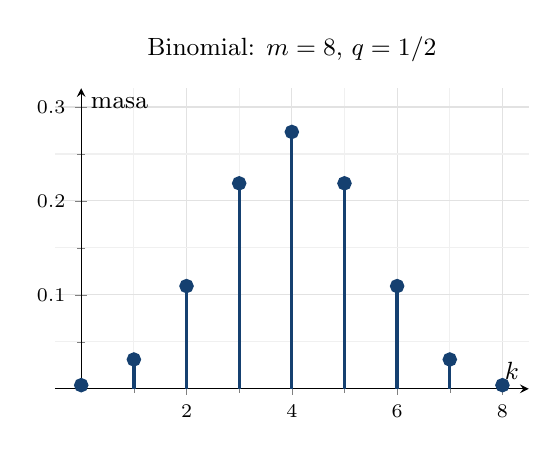
\begin{tikzpicture}\begin{axis}[base,width=7.6cm,height=5.4cm,xlabel={$k$},ylabel={masa},xmin=-.5,xmax=8.5,ymin=0,ymax=.32,ytick={0,.1,.2,.3},title={Binomial: $m=8$, $q=1/2$},title style={font=\small}]
\addplot[ycomb,azul,very thick,mark=*]coordinates{(0,.00390625)(1,.03125)(2,.109375)(3,.21875)(4,.2734375)(5,.21875)(6,.109375)(7,.03125)(8,.00390625)};
\end{axis}\end{tikzpicture}\hfill
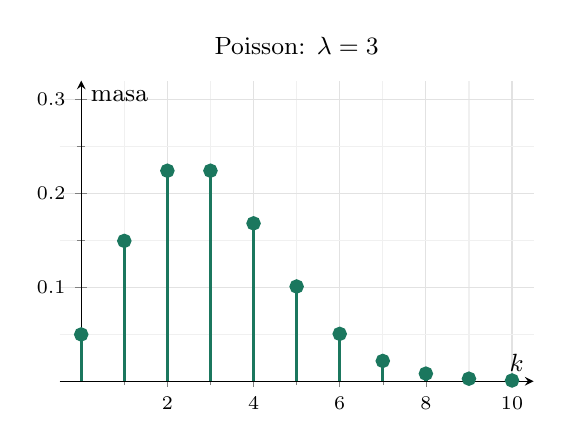
\begin{tikzpicture}\begin{axis}[base,width=7.6cm,height=5.4cm,xlabel={$k$},ylabel={masa},xmin=-.5,xmax=10.5,ymin=0,ymax=.32,title={Poisson: $\lambda=3$},title style={font=\small}]
\addplot[ycomb,verde,very thick,mark=*]coordinates{(0,.049787)(1,.149361)(2,.224042)(3,.224042)(4,.168031)(5,.100819)(6,.050409)(7,.021604)(8,.008102)(9,.002701)(10,.000810)};
\end{axis}\end{tikzpicture}
\caption{Una masa es la altura de un punto discreto. Los segmentos solo ayudan a comparar probabilidades; no son una densidad continua.}
\end{figure}

\section{Distribuciones continuas: uniforme, exponencial, gamma y beta}
\subsection{Uniforme y cambio de escala}
Si $U\sim\mathrm{Unif}[a,b]$, $a<b$, $f_U(u)=1/(b-a)$ en ese intervalo. Integrando,
\[
\E U=\frac1{b-a}\left[\frac{u^2}2\right]_a^b=\frac{a+b}2,
\quad\E U^2=\frac{a^2+ab+b^2}3,
\quad\Var(U)=\frac{(b-a)^2}{12}.
\]
Si $V=g(U)$ y $g$ es estrictamente monótona y diferenciable con inversa diferenciable,
\[
f_V(v)=f_U(g^{-1}(v))\left|\frac{\mathrm d}{\mathrm dv}g^{-1}(v)\right|.
\]
Esta fórmula se deduce transformando $\Prob(v<V<v+\Delta v)$ y dividiendo por $\Delta v$. Para transformaciones con varias ramas inversas se suman las contribuciones de todas las ramas.
\subsection{Exponencial y falta de memoria}
La densidad $f_T(t)=\lambda e^{-\lambda t}\ind_{\{t\ge0\}}$ integra uno. Su supervivencia es $\Prob(T>t)=e^{-\lambda t}$ para $t\ge0$, y
\[
\Prob(T>s+t\mid T>s)=\frac{e^{-\lambda(s+t)}}{e^{-\lambda s}}=e^{-\lambda t}.
\]
Integración por partes da $\E T=1/\lambda$ y $\E T^2=2/\lambda^2$, por tanto $\Var(T)=1/\lambda^2$. Su generadora $M_T(t)=\lambda/(\lambda-t)$ solo existe para $t<\lambda$.
\subsection{Gamma: extender factoriales mediante una integral}
Definimos $\Gamma(a)=\int_0^\infty u^{a-1}e^{-u}\dd u$ para $a>0$. Por partes, $\Gamma(a+1)=a\Gamma(a)$ y $\Gamma(1)=1$, así que $\Gamma(m)=(m-1)!$ para entero positivo. La densidad gamma de forma $a$ y \emph{tasa} $\lambda$ es
\[
f_T(t)=\frac{\lambda^a}{\Gamma(a)}t^{a-1}e^{-\lambda t}\ind_{\{t>0\}}.
\]
Usando $u=\lambda t$, para $s>-a$,
\[
\E T^s=\lambda^{-s}\frac{\Gamma(a+s)}{\Gamma(a)},\qquad
\E T=\frac a\lambda,\quad\Var(T)=\frac a{\lambda^2}.
\]
La suma de $m$ exponenciales independientes de tasa común es gamma $(m,\lambda)$: su generadora es $[\lambda/(\lambda-t)]^m$. Tasa y escala son recíprocas; una fórmula escrita en escala $\theta=1/\lambda$ tiene media $a\theta$ y varianza $a\theta^2$.
\subsection{Beta: probabilidades aleatorias}
Para $a,b>0$, sea $B(a,b)=\int_0^1u^{a-1}(1-u)^{b-1}\dd u$. El cambio $(s,t)=(rv,r(1-v))$ en $\Gamma(a)\Gamma(b)$, con Jacobiano $r$, produce
\[
B(a,b)=\frac{\Gamma(a)\Gamma(b)}{\Gamma(a+b)}.
\]
Una beta tiene densidad $u^{a-1}(1-u)^{b-1}/B(a,b)$ en $(0,1)$. Entonces
\[
\E U^s=\frac{B(a+s,b)}{B(a,b)},\quad
\E U=\frac a{a+b},\quad
\Var(U)=\frac{ab}{(a+b)^2(a+b+1)}.
\]
La varianza se obtiene restando $a^2/(a+b)^2$ de $a(a+1)/[(a+b)(a+b+1)]$. Si $Q$ es beta y $K\mid Q$ binomial $(m,Q)$, $\E K=m\E Q$ y
\[
\Var(K)=m\E[Q(1-Q)]+m^2\Var(Q).
\]
La heterogeneidad de $Q$ añade variabilidad frente a una binomial con parámetro fijo $\E Q$.
\begin{figure}[H]\centering
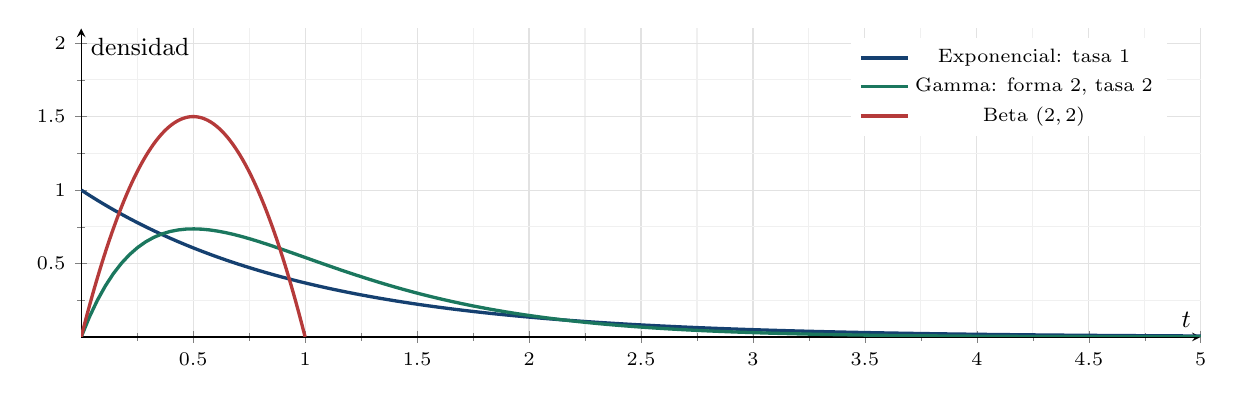
\begin{tikzpicture}\begin{axis}[base,width=15.8cm,height=5.5cm,xmin=0,xmax=5,ymin=0,ymax=2.1,xlabel={$t$},ylabel={densidad},legend pos=north east]
\addplot[azul,very thick,domain=0:5]{exp(-x)};\addlegendentry{Exponencial: tasa $1$}
\addplot[verde,very thick,domain=0:5]{4*x*exp(-2*x)};\addlegendentry{Gamma: forma $2$, tasa $2$}
\addplot[rojo,very thick,domain=0:1,samples=100]{6*x*(1-x)};\addlegendentry{Beta $(2,2)$}
\end{axis}\end{tikzpicture}
\caption{Las áreas totales son uno, aunque las alturas y los soportes cambien. Las tres densidades son fórmulas exactas, no ajustes de una muestra.}
\end{figure}

\section{Normal escalar: integral gaussiana, momentos y transformaciones}
\subsection{La constante de normalización no se memoriza}
Sea $I=\int_\R e^{-u^2/2}\dd u$. El integrando es no negativo y podemos formar
\[
I^2=\iint_{\R^2}e^{-(u^2+v^2)/2}\dd u\dd v.
\]
En coordenadas polares $u=r\cos\theta$, $v=r\sin\theta$, el elemento de área es $r\dd r\dd\theta$. Por tanto,
\[
I^2=\int_0^{2\pi}\int_0^\infty e^{-r^2/2}r\dd r\dd\theta=2\pi,
\qquad I=\sqrt{2\pi}.
\]
Definimos $Z\sim\mathcal N(0,1)$ mediante $\phi(z)=(2\pi)^{-1/2}e^{-z^2/2}$ y $\Phi(t)=\int_{-\infty}^t\phi(z)\dd z$. La simetría da $\E Z=0$. Como $\phi'(z)=-z\phi(z)$,
\[
\E Z^2=-\int_\R z\phi'(z)\dd z
=-[z\phi(z)]_{-\infty}^{\infty}+\int_\R\phi(z)\dd z=1.
\]
Más generalmente, los momentos impares son cero y $\E Z^{2m}=(2m-1)\E Z^{2m-2}$ por partes. Así, $\E Z^4=3$, $\E Z^6=15$.
\subsection{Completar cuadrados y la generadora}
\[
M_Z(t)=\frac1{\sqrt{2\pi}}\int_\R e^{tz-z^2/2}\dd z
=e^{t^2/2}\frac1{\sqrt{2\pi}}\int_\R e^{-(z-t)^2/2}\dd z=e^{t^2/2}.
\]
Para $U=\mu+\sigma Z$, $\sigma>0$,
\[
f_U(u)=\frac1{\sigma\sqrt{2\pi}}\exp\!\left[-\frac{(u-\mu)^2}{2\sigma^2}\right],
\quad M_U(t)=e^{\mu t+\sigma^2t^2/2},
\quad\E U=\mu,\quad\Var(U)=\sigma^2.
\]
La suma de normales \emph{independientes} es normal porque se multiplican las generadoras. Para normales marginales dependientes no basta conocer las distribuciones individuales: necesitaremos normalidad conjunta.
\subsection{Cuadrados gaussianos y chi-cuadrado}
Si $Q=Z^2$, las ramas $z=\pm\sqrt q$ tienen derivada absoluta $1/(2\sqrt q)$. Sumarlas da
\[
f_Q(q)=\frac{q^{-1/2}e^{-q/2}}{\sqrt{2\pi}},\quad q>0.
\]
Esta es una gamma de forma $1/2$ y tasa $1/2$, porque $\Gamma(1/2)=\sqrt\pi$, identidad equivalente a la integral gaussiana. Si $Z_1,\ldots,Z_\nu$ son independientes estándar,
\[
Q=\sum_{i=1}^\nu Z_i^2\sim\chi^2_\nu,\quad
M_Q(t)=(1-2t)^{-\nu/2},\quad
\E Q=\nu,\quad\Var(Q)=2\nu.
\]
Los grados de libertad $\nu$ cuentan términos gaussianos independientes que se elevan al cuadrado. Más adelante una proyección matricial explicará por qué estimar $p$ coeficientes deja $n-p$ grados de libertad.
\subsection{Lognormal: transformar una normal no conserva su media}
Para $V=e^U$, $U\sim\mathcal N(\mu,\sigma^2)$,
\[
\E V^k=M_U(k)=e^{k\mu+k^2\sigma^2/2},\quad
\E V=e^{\mu+\sigma^2/2},\quad
\Var(V)=(e^{\sigma^2}-1)e^{2\mu+\sigma^2}.
\]
En particular $\E(e^U)\ne e^{\E U}$ cuando $\sigma>0$. La lognormal tiene todos los momentos positivos finitos, pero $\E(e^{tV})=\infty$ para $t>0$: tener momentos no garantiza una generadora finita alrededor de cero.

\section{Student, Fisher y colas: cuándo los momentos dejan de existir}
Sean $Z\sim\mathcal N(0,1)$ y $Q\sim\chi^2_\nu$ independientes. La variable
\[
T=\frac{Z}{\sqrt{Q/\nu}}
\]
introduce una escala aleatoria. El cambio $z=t\sqrt{q/\nu}$ tiene Jacobiano $\sqrt{q/\nu}$. Integrando la densidad conjunta sobre $q>0$,
\begin{align*}
f_T(t)&=\int_0^\infty \phi(t\sqrt{q/\nu})
\frac{q^{\nu/2-1}e^{-q/2}}{2^{\nu/2}\Gamma(\nu/2)}\sqrt{q/\nu}\dd q\\
&=\frac{\Gamma((\nu+1)/2)}{\sqrt{\nu\pi}\Gamma(\nu/2)}
\left(1+\frac{t^2}{\nu}\right)^{-(\nu+1)/2}.
\end{align*}
La cola es de orden $|t|^{-\nu-1}$: $\E|T|^s<\infty$ si y solo si $s<\nu$. Por simetría $\E T=0$ si $\nu>1$. Para $\nu>2$, independencia y los momentos negativos de la gamma dan
\[
\Var(T)=\E Z^2\cdot\nu\E(Q^{-1})
=\nu\frac{1/2}{\nu/2-1}=\frac\nu{\nu-2}.
\]
Con $\nu=1$, Student es Cauchy: $f(t)=1/[\pi(1+t^2)]$. Su esperanza \emph{no existe}; el valor principal simétrico cero no es una esperanza. Con $1<\nu\le2$, sí existe la media, pero no la varianza finita.
\subsection{Fisher como cociente de dos energías}
Si $Q_1\sim\chi^2_a$, $Q_2\sim\chi^2_b$ son independientes,
\[
F=\frac{Q_1/a}{Q_2/b}\sim F_{a,b}.
\]
Transformando $(Q_1,Q_2)$ a $(F,Q_2)$ e integrando el segundo componente se obtiene
\[
f_F(f)=\frac{(a/b)^{a/2}}{B(a/2,b/2)}
f^{a/2-1}(1+af/b)^{-(a+b)/2},\qquad f>0.
\]
Su media existe para $b>2$ y vale $b/(b-2)$. Para $b>4$,
\[
\Var(F)=\frac{2b^2(a+b-2)}{a(b-2)^2(b-4)}.
\]
También $T_\nu^2\sim F_{1,\nu}$. Las condiciones sobre grados de libertad son parte de la fórmula, no notas opcionales.
\begin{figure}[H]\centering
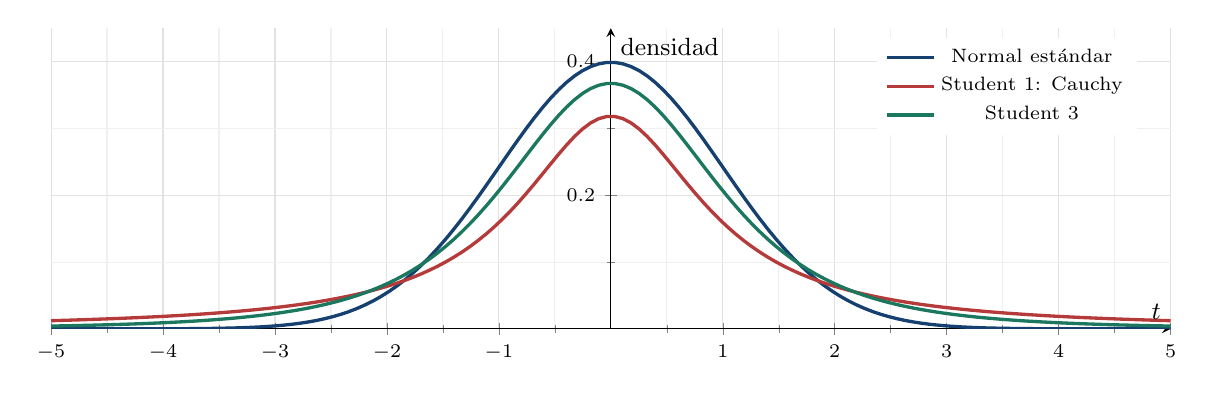
\begin{tikzpicture}\begin{axis}[base,width=15.8cm,height=5.4cm,xmin=-5,xmax=5,ymin=0,ymax=.45,xlabel={$t$},ylabel={densidad},legend pos=north east]
\addplot[azul,very thick,domain=-5:5]{exp(-x*x/2)/sqrt(2*pi)};\addlegendentry{Normal estándar}
\addplot[rojo,very thick,domain=-5:5]{1/(pi*(1+x*x))};\addlegendentry{Student $1$: Cauchy}
\addplot[verde,very thick,domain=-5:5]{2/(pi*sqrt(3))*(1+x*x/3)^(-2)};\addlegendentry{Student $3$}
\end{axis}\end{tikzpicture}
\caption{Un centro parecido no implica colas parecidas. La normal tiene todos sus momentos; Cauchy carece incluso de esperanza.}
\end{figure}
\begin{idea}[Cuadro de condiciones antes de calcular]
Antes de escribir $\E U$, comprobar $\E|U|<\infty$; antes de escribir una covarianza, comprobar segundos momentos. Antes de dividir por una variable aleatoria, estudiar si puede acercarse a cero. Esta última cuestión será decisiva para variables instrumentales y estimadores de razón.
\end{idea}

\parte{II. Espacios vectoriales, normas y métricas: de dos a miles de dimensiones}
\section{Qué es un vector: objeto, operaciones y coordenadas}
Un vector de $\R^p$ es una lista ordenada $x=(x_1,\ldots,x_p)\T$. Sumamos por coordenadas y multiplicamos por escalares:
\[
(x+y)_j=x_j+y_j,\qquad (ax)_j=ax_j,\qquad j=1,\ldots,p.
\]
Si $x=(2,-1)\T$, $y=(3,4)\T$ y $a=-2$, entonces $x+y=(5,3)\T$ y $ax=(-4,2)\T$. En $\R^{10000}$ se hacen exactamente las mismas operaciones, con $10000$ entradas. La imposibilidad de dibujarlas todas no cambia sus definiciones.
\subsection{Los ocho axiomas y por qué importan}
Un espacio vectorial $V$ sobre $\R$ contiene una suma $V\times V\to V$ y una multiplicación $\R\times V\to V$. Para $u,v,w\in V$ y $a,b\in\R$, exige
\begin{align*}
u+v&=v+u,& (u+v)+w&=u+(v+w),& u+0&=u,&u+(-u)&=0,\\
a(u+v)&=au+av,&(a+b)u&=au+bu,&a(bu)&=(ab)u,&1u&=u.
\end{align*}
Las operaciones deben además quedar dentro de $V$. De los axiomas salen $0u=0$ y $a0=0$: por ejemplo $0u=(0+0)u=0u+0u$, y restar $0u$ da el resultado. El vector cero es único porque, si $0'$ también es neutro, $0=0+0'=0'$. Estos hechos sostienen todas las manipulaciones de sistemas lineales.
\subsection{Espacios que no son flechas físicas}
\begin{enumerate}
\item $\R^{n\times p}$ con suma y escala entrada por entrada tiene dimensión $np$.
\item $\mathcal P_d=\{a_0+a_1t+\cdots+a_dt^d\}$ tiene dimensión $d+1$ y base $1,t,\ldots,t^d$.
\item Las matrices simétricas $p\times p$ forman un espacio de dimensión $p(p+1)/2$: elegimos la diagonal y las entradas por encima de ella.
\item Las funciones continuas en $[0,1]$ forman un espacio vectorial infinito dimensional; los monomios $1,t,t^2,\ldots$ ya contienen familias independientes de cualquier tamaño.
\end{enumerate}
Las matrices \emph{positivas definidas} no forman un espacio vectorial: si $A$ es positiva definida, $-A$ no lo es. Los vectores de probabilidades tampoco: deben sumar uno y no admiten todos los múltiplos escalares.
\subsection{Subespacios frente a espacios afines}
Un subconjunto $W\subseteq V$ es subespacio si contiene cero y si $au+bv\in W$ para todo $u,v\in W$ y $a,b\in\R$. En $\R^3$, $W=\{x:x_1+x_2+x_3=0\}$ es un plano vectorial. El conjunto $A=\{x:x_1+x_2+x_3=1\}$ es afín: se escribe $a+W$, pero no contiene cero.
\begin{ejemplo}[Un plano en mil dimensiones sin dibujo]
En $\R^{1000}$,
\[
W=\left\{x:\sum_{j=1}^{1000}x_j=0\right\}
=\spanop\{e_1-e_{1000},\ldots,e_{999}-e_{1000}\}.
\]
Los $999$ vectores son independientes: las primeras $999$ coordenadas de una combinación nula obligan a anular cada coeficiente. Cualquier $x\in W$ se reconstruye con esos coeficientes $x_1,\ldots,x_{999}$ porque $x_{1000}=-\sum_{j<1000}x_j$. Por eso $\dim W=999$.
\end{ejemplo}

\section{Independencia, bases, dimensión y sistemas de ecuaciones}
Una combinación lineal es $\sum_{j=1}^k a_jv_j$. El conjunto de todas esas combinaciones es $\spanop\{v_1,\ldots,v_k\}$. Los vectores son linealmente independientes si $\sum_j a_jv_j=0$ solo admite $a_1=\cdots=a_k=0$. Una base es una familia independiente que genera todo el espacio.
\begin{deduccion}
Si $v_1,\ldots,v_k$ forman una base y $x=\sum_j a_jv_j=\sum_j b_jv_j$, restar da $\sum_j(a_j-b_j)v_j=0$. Por independencia $a_j=b_j$. Las coordenadas en una base son únicas. Si una familia generadora tiene un vector que es combinación de los demás, se puede eliminar sin cambiar el espacio generado; repitiendo, se obtiene una base finita.
\end{deduccion}
La dimensión es el número de vectores de una base; el lema de intercambio asegura que todas las bases finitas tienen el mismo tamaño. Su idea constructiva es sustituir sucesivamente un generador por un vector independiente nuevo, resolviendo una combinación con un coeficiente no nulo. Una familia independiente no puede ser más larga que una generadora.
\subsection{Cambiar la base cambia coordenadas, no el objeto}
Si $B=[b_1\ \cdots\ b_p]$ es invertible, $x=Bc$ y $c=B^{-1}x$. Para
\[
B=\begin{pmatrix}1&1\\0&1\end{pmatrix},\quad x=\begin{pmatrix}3\\2\end{pmatrix},
\qquad c=\begin{pmatrix}1\\2\end{pmatrix}.
\]
El objeto es el mismo, pero la primera coordenada cambia de $3$ a $1$. En una base oblicua, $c\T c$ no representa la longitud euclidiana de $x$: $\norm{x}_2^2=c\T B\T Bc$. El producto $B\T B$ es la matriz de Gram de esa base.
\subsection{Transformaciones lineales, núcleo y rango}
Una aplicación $T:V\to W$ es lineal si $T(au+bv)=aT(u)+bT(v)$. En bases finitas la representa una matriz $A\in\R^{m\times p}$:
\[
(Ax)_i=\sum_{j=1}^p a_{ij}x_j.
\]
Su núcleo es $\kerop A=\{x:Ax=0\}$ y su imagen $\range A=\{Ax:x\in\R^p\}$. El rango es $\dim(\range A)$.
\begin{teorema}[Rango más nulidad]
Para $A\in\R^{m\times p}$, $\rank A+\dim(\kerop A)=p$.
\end{teorema}
\begin{deduccion}
Toma una base $v_1,\ldots,v_d$ del núcleo y extiéndela a una base $v_1,\ldots,v_p$ del dominio. Los vectores $Av_{d+1},\ldots,Av_p$ generan la imagen porque los primeros $d$ se anulan. Son independientes: si $\sum_{j>d}c_jAv_j=0$, el vector $\sum_{j>d}c_jv_j$ está en el núcleo y puede escribirse con $v_1,\ldots,v_d$. La independencia de la base completa obliga a que todos los $c_j$ sean cero. La imagen tiene dimensión $p-d$.
\end{deduccion}
Así, $Ax=b$ admite solución si y solo si $b\in\range A$. Si $x_0$ es una solución, todas son $x_0+\kerop A$. La eliminación gaussiana aplica operaciones reversibles a filas, conservando soluciones y exhibiendo pivotes. Un pivote por columna implica unicidad de una solución existente.
\begin{ejemplo}[Un sistema subdeterminado]
\[
A=\begin{pmatrix}1&1&0\\0&1&1\end{pmatrix},\quad b=(2,3)\T.
\]
Las ecuaciones son $x_1+x_2=2$, $x_2+x_3=3$. Con $x_2=t$,
\[
x=(2,0,3)\T+t(-1,1,-1)\T.
\]
El rango es dos y el núcleo tiene dimensión uno. En alta dimensión, $n<p$ produce el mismo fenómeno en regresión: varias colecciones de coeficientes pueden generar las mismas predicciones.
\end{ejemplo}

\section{Producto interno, ángulos y ortogonalidad con pruebas}
Un producto interno real es una función $\ip uv$ simétrica, bilineal y positiva: $\ip xx\ge0$, con igualdad solo si $x=0$. En $\R^p$, $\ip xy=x\T y=\sum_jx_jy_j$ es el producto euclidiano; su norma es $\norm x_2=\sqrt{x\T x}$.
\begin{teorema}[Cauchy--Schwarz y desigualdad triangular]
Para un producto interno, $|\ip xy|\le\norm x\norm y$ y $\norm{x+y}\le\norm x+\norm y$.
\end{teorema}
\begin{deduccion}
Si $y\ne0$, la cantidad $\norm{x-ty}^2=\norm x^2-2t\ip xy+t^2\norm y^2$ es no negativa para todo $t$. Eligiendo $t=\ip xy/\norm y^2$ obtenemos $\norm x^2-(\ip xy)^2/\norm y^2\ge0$. La igualdad exige $x$ múltiplo de $y$. Ahora
\[
\norm{x+y}^2=\norm x^2+2\ip xy+\norm y^2
\le(\norm x+\norm y)^2.
\]
Tomar raíces termina la prueba.
\end{deduccion}
Para vectores no nulos, $\cos\theta=x\T y/(\norm x_2\norm y_2)$ define el ángulo $\theta\in[0,\pi]$. Si el producto interno vale cero, son ortogonales y $\norm{x+y}_2^2=\norm x_2^2+\norm y_2^2$.
\subsection{Gram--Schmidt, paso por paso}
Partiendo de vectores independientes $a_1,\ldots,a_k$, definimos
\[
q_1=\frac{a_1}{\norm{a_1}_2},\quad
r_j=a_j-\sum_{i<j}(q_i\T a_j)q_i,\quad q_j=\frac{r_j}{\norm{r_j}_2}.
\]
Entonces $q_i\T r_j=0$ para $i<j$; independencia asegura $r_j\ne0$. Cada $q_j$ pertenece al espacio generado por $a_1,\ldots,a_j$, y ambos conjuntos generan el mismo subespacio. Para $A=[a_1\ \cdots\ a_k]$ obtenemos $A=QR$, $Q\T Q=I_k$, $R$ triangular superior.
\begin{ejemplo}[Una base ortogonal de un plano en tres coordenadas]
Con $a_1=(1,1,0)\T$, $a_2=(1,0,1)\T$,
\[
q_1=\frac{(1,1,0)\T}{\sqrt2},\quad
r_2=(1/2,-1/2,1)\T,\quad
q_2=\frac{(1,-1,2)\T}{\sqrt6}.
\]
Así, $R=\begin{psmallmatrix}\sqrt2&1/\sqrt2\\0&\sqrt{3/2}\end{psmallmatrix}$. Para $x=(2,1,3)\T$, sus coordenadas sobre ese plano son $q_1\T x=3/\sqrt2$, $q_2\T x=7/\sqrt6$. La proyección es la suma de esas coordenadas multiplicadas por sus ejes; el residuo es ortogonal a ambos.
\end{ejemplo}

\begin{figure}[H]\centering
\tdplotsetmaincoords{66}{40}
\begin{tikzpicture}[tdplot_main_coords,scale=1.2]
\fill[celeste,opacity=.8](-.5,-.5,0)--(3.3,-.5,0)--(3.3,2.4,0)--(-.5,2.4,0)--cycle;
\draw[gray!45](-.5,-.5,0)--(3.3,-.5,0)--(3.3,2.4,0)--(-.5,2.4,0)--cycle;
\draw[eje](0,0,0)--(4,0,0)node[anchor=north east]{$x_1$};
\draw[eje](0,0,0)--(0,3,0)node[anchor=north west]{$x_2$};
\draw[eje](0,0,0)--(0,0,3.7)node[above]{$x_3$};
\draw[vec](0,0,0)--(2,1,3)node[above right]{$x=(2,1,3)\T$};
\draw[vecverde](0,0,0)--(2,1,0)node[below right]{$Px=(2,1,0)\T$};
\draw[vecrojo](2,1,0)--(2,1,3)node[midway,right]{$e=(0,0,3)\T$};
\node[azul,anchor=east]at(-.8,-1,0){$W:\ x_3=0$};
\end{tikzpicture}
\caption{Proyección en tres dimensiones: $\norm x_2^2=14=5+9=\norm{Px}_2^2+\norm e_2^2$. En dimensión grande cambian las coordenadas, pero la identidad de Pitágoras es la misma.}
\end{figure}

\subsection{El dual: un vector también puede codificar una medición}
Un funcional lineal $\ell:V\to\R$ devuelve un escalar. En $\R^p$ toda medición lineal es $\ell(x)=a\T x$. El espacio de funcionales es el dual $V^*$. El producto interno permite identificar un vector $a$ con ese funcional; cambiar el producto interno cambia la identificación. Un gradiente es precisamente el vector que representa una derivada lineal mediante el producto interno elegido.

\section{Normas: longitud sin exigir un producto interno}
Una norma es una función $\norm\cdot:V\to[0,\infty)$ con positividad estricta fuera de cero, homogeneidad $\norm{ax}=|a|\norm x$ y desigualdad triangular. En $\R^p$,
\[
\norm x_q=\left(\sum_{j=1}^p|x_j|^q\right)^{1/q},\quad 1\le q<\infty,
\qquad\norm x_\infty=\max_j|x_j|.
\]
Para $x=(3,-4)\T$, las normas $1,2,\infty$ valen $7,5,4$. $\norm x_0=\#\{j:x_j\ne0\}$ suele llamarse ``norma cero'', pero no es una norma: $\norm{2x}_0=\norm x_0$, violando homogeneidad.
\subsection{Hölder y Minkowski sin saltar la desigualdad clave}
Si $q,r>1$, $1/q+1/r=1$, la desigualdad de Young $ab\le a^q/q+b^r/r$ para $a,b\ge0$ sale de maximizar $ab-a^q/q$ respecto a $a$: el máximo en $a=b^{r-1}$ vale $b^r/r$. Normalizar las secuencias por sus normas y sumar Young da
\[
\sum_j|u_jv_j|\le\norm u_q\norm v_r.
\]
Si $s=u+v$ y $\norm s_q>0$, entonces
\begin{align*}
\norm s_q^q&\le\sum_j(|u_j|+|v_j|)|s_j|^{q-1}\\
&\le(\norm u_q+\norm v_q)
\left(\sum_j|s_j|^{(q-1)r}\right)^{1/r}
=(\norm u_q+\norm v_q)\norm s_q^{q-1}.
\end{align*}
Dividir prueba Minkowski. Para $q=1$ basta $|u_j+v_j|\le|u_j|+|v_j|$; para $q=\infty$, tomar el máximo de esa desigualdad.
\subsection{Comparar normas cuando crece la dimensión}
Si $1\le q<r\le\infty$,
\[
\norm x_r\le\norm x_q\le p^{1/q-1/r}\norm x_r.
\]
La primera se deduce normalizando $\norm x_q=1$: cada $|x_j|\le1$ y $|x_j|^r\le|x_j|^q$. La segunda se obtiene con Hölder aplicado a $\sum_j|x_j|^q\cdot1$. Para $x=\ones_p$, $\norm x_1=p$, $\norm x_2=\sqrt p$, $\norm x_\infty=1$. En $p=10000$ valen $10000,100,1$; son tres objetivos geométricos distintos.
\subsection{La norma dual y el máximo de una combinación}
Definimos $\norm a_* =\sup_{\norm x\le1}a\T x$. La dual de $\norm\cdot_q$ es $\norm\cdot_r$. Para $1<q<\infty$, Hölder da la cota y la elección $x_j\propto\sign(a_j)|a_j|^{r-1}$ la alcanza. Para $q=1$, concentrar $x$ en una coordenada de máximo $|a_j|$ da $\norm a_\infty$. Para $q=\infty$, elegir $x_j=\sign(a_j)$ da $\norm a_1$. Este hecho reaparece en regularización y dualidad convexa.
\begin{figure}[H]\centering
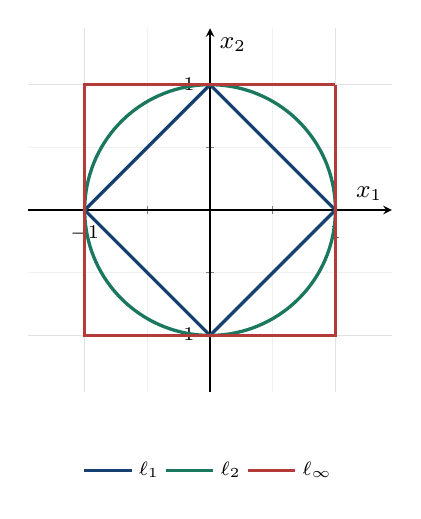
\begin{tikzpicture}\begin{axis}[base,width=7.7cm,height=6.2cm,axis equal image,xmin=-1.45,xmax=1.45,ymin=-1.45,ymax=1.45,xlabel={$x_1$},ylabel={$x_2$},legend style={at={(.5,-.16)},anchor=north,legend columns=3}]
\addplot[azul,very thick]coordinates{(1,0)(0,1)(-1,0)(0,-1)(1,0)};\addlegendentry{$\ell_1$}
\addplot[verde,very thick,domain=0:360]({cos(x)},{sin(x)});\addlegendentry{$\ell_2$}
\addplot[rojo,very thick]coordinates{(1,1)(-1,1)(-1,-1)(1,-1)(1,1)};\addlegendentry{$\ell_\infty$}
\end{axis}\end{tikzpicture}\hfill
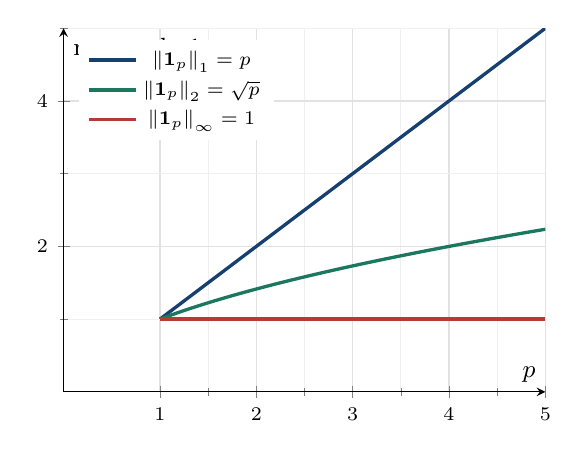
\begin{tikzpicture}\begin{axis}[base,width=7.7cm,height=6.2cm,xmin=0,xmax=5,ymin=0,ymax=5,xlabel={$p$},ylabel={norma de $\ones_p$},legend pos=north west,xtick={1,2,3,4,5}]
\addplot[azul,very thick,domain=1:5]{x};\addlegendentry{$\norm{\ones_p}_1=p$}
\addplot[verde,very thick,domain=1:5]{sqrt(x)};\addlegendentry{$\norm{\ones_p}_2=\sqrt p$}
\addplot[rojo,very thick,domain=1:5]{1};\addlegendentry{$\norm{\ones_p}_\infty=1$}
\end{axis}\end{tikzpicture}
\caption{Izquierda: fronteras de bolas unitarias. Derecha: fórmulas evaluadas en dimensiones enteras; las curvas entre enteros son guías de comparación.}
\end{figure}

\section{Métricas, pseudométricas y distancias que parecen serlo}
Una métrica $d:V\times V\to[0,\infty)$ satisface $d(x,y)=0$ si y solo si $x=y$, simetría y $d(x,z)\le d(x,y)+d(y,z)$. Cualquier norma genera $d(x,y)=\norm{x-y}$. Una \emph{pseudométrica} permite distancia cero entre objetos diferentes.
\begin{center}\small
\begin{tabular}{>{\raggedright\arraybackslash}p{3.0cm}>{\raggedright\arraybackslash}p{6.3cm}>{\raggedright\arraybackslash}p{6.0cm}}\toprule
Nombre & Fórmula & Condición o interpretación\\\midrule
Euclidiana & $\sqrt{\sum_j(x_j-y_j)^2}$ & Métrica; combina diferencias por energía.\\
Manhattan & $\sum_j|x_j-y_j|$ & Métrica; suma cambios absolutos.\\
Chebyshev & $\max_j|x_j-y_j|$ & Métrica; controla el peor cambio.\\
Hamming & $\sum_j\ind_{\{x_j\ne y_j\}}$ & Métrica sobre cadenas de igual longitud.\\
Mahalanobis & $\sqrt{(x-y)\T G(x-y)}$ & Métrica si $G\succ0$.\\
Euclidiana cuadrada & $\sum_j(x_j-y_j)^2$ & No cumple triangular en general.\\
Disimilitud coseno & $1-x\T y/(\norm x_2\norm y_2)$ & No es métrica en vectores no nulos.\\
Angular & $\arccos(x\T y/(\norm x_2\norm y_2))$ & Métrica en la esfera unitaria.\\\bottomrule
\end{tabular}
\end{center}
\subsection{Contraejemplos que evitan confundir pérdidas y distancias}
En $\R$, la distancia cuadrada entre $0$ y $2$ vale $4$, pero entre $0,1$ y $1,2$ suma $2$: falla triangular. Para vectores unitarios de ángulos $0^\circ,60^\circ,120^\circ$, la disimilitud coseno entre extremos vale $1.5$, mientras las otras dos suman $0.5+0.5=1$. Además, $x$ y $2x$ tienen disimilitud coseno cero aunque sean distintos.
La distancia $\norm{x/\norm x_2-y/\norm y_2}_2$ es una métrica sobre direcciones normalizadas porque es euclidiana en la esfera. Si se aplica a vectores originales, es una pseudométrica respecto a múltiplos positivos.
\subsection{Distancias entre distribuciones}
Para masas sobre un conjunto finito,
\[
d_{\rm TV}(p,q)=\frac12\sum_j|p_j-q_j|
\]
es una métrica: es la mitad de una norma $\ell_1$. En cambio,
\[
D_{\rm KL}(p\Vert q)=\sum_{j:p_j>0}p_j\log(p_j/q_j)
\]
es una divergencia, con valor infinito si $p_j>0,q_j=0$. No es simétrica ni triangular. Su no negatividad sale de $-\log t\ge1-t$:
\[
\sum_{j:p_j>0}-p_j\log(q_j/p_j)\ge
\sum_{j:p_j>0}(p_j-q_j)\ge0.
\]
La desigualdad $-\log t\ge1-t$ se verifica derivando $t-1-\log t$: su mínimo está en uno. Distinguir divergencia, pérdida y métrica evita exigir a KL o al error cuadrático propiedades que no tienen.

\section{Métricas matriciales, elipsoides y singularidad}
Si $G=G\T\succ0$, definimos $\ip xy_G=x\T Gy$ y $\norm x_G=\sqrt{x\T Gx}$. Positividad definida significa $x\T Gx>0$ para $x\ne0$. Las demás propiedades de producto interno salen de la simetría y de la bilinealidad del producto matricial. Por Cauchy--Schwarz, $\norm\cdot_G$ satisface triangular.
\subsection{Descomponer una forma cuadrática}
Con $G=Q\Lambda Q\T$, $Q$ ortogonal y $\Lambda=\diag(g_1,\ldots,g_p)$ con $g_j>0$, sea $L=\Lambda^{1/2}Q\T$. Entonces
\[
G=L\T L,\qquad d_G(x,y)=\norm{L(x-y)}_2.
\]
Una métrica ponderada equivale a transformar coordenadas y medir después con Euclides. La bola $x\T Gx\le1$ tiene semiejes $1/\sqrt{g_j}$ en las direcciones $q_j$. Los pesos grandes hacen costosa una diferencia pequeña sobre ese eje.
\subsection{Mahalanobis: corregir escala y correlación}
Para una covarianza invertible $\Sigma$, $d_M(x,y)^2=(x-y)\T\Sigma^{-1}(x-y)$. Si $\Sigma=\diag(\sigma_1^2,\ldots,\sigma_p^2)$, entonces $d_M^2=\sum_j[(x_j-y_j)/\sigma_j]^2$. Si hay correlaciones, estandarizar por desviaciones marginales no basta: hay que rotar además hacia los ejes propios.
\begin{ejemplo}[Dos diferencias iguales en Euclides y muy distintas en riesgo]
\[
\Sigma=\begin{pmatrix}4&3\\3&4\end{pmatrix},\quad
\Sigma^{-1}=\frac17\begin{pmatrix}4&-3\\-3&4\end{pmatrix}.
\]
Para $u=(1,1)\T$ y $v=(1,-1)\T$, $\norm u_2^2=\norm v_2^2=2$, pero
\[
u\T\Sigma^{-1}u=\frac27,\qquad v\T\Sigma^{-1}v=2.
\]
La primera diferencia sigue una dirección de alta variación conjunta; la segunda va contra ella y es siete veces mayor en distancia cuadrada estandarizada.
\end{ejemplo}
\subsection{Una matriz semidefinida induce pseudométrica}
Si $G\succeq0$ es singular, existe $h\ne0$ con $Gh=0$ y $d_G(x,x+h)=0$. Para $G=\diag(1,0)$, los puntos $(0,0)\T$ y $(0,10)\T$ tienen distancia cero. Se puede trabajar en el cociente $\R^p/\kerop G$, donde esos puntos se identifican, o restringir al subespacio de autovalores positivos.
La pseudoinversa $\Sigma^+$ invierte solo autovalores positivos. Para una distribución normal singular, su soporte afín es $\mu+\range\Sigma$. En ese soporte, $\Sigma^+$ define una métrica; fuera del soporte, una fórmula con pseudoinversa puede ignorar desplazamientos imposibles bajo el modelo.
\subsection{Dimensión grande y coste de construir la distancia}
Una matriz densa $p\times p$ necesita $p^2$ números; con $p=10000$, $10^8$ entradas son unos $800$ MB en doble precisión, antes de copias auxiliares. Una diagonal requiere $p$ números, y una estructura $D+BB\T$ con $B\in\R^{p\times k}$ requiere $p+pk$. Elegir una métrica no solo cambia geometría: determina memoria, cálculo y qué estructura estadística podemos estimar.

\parte{III. Geometría espectral: direcciones, transformaciones y proyecciones}
\section{Dimensión, coordenadas y la necesidad de reducir}
Una observación con $p$ características es $x_i=(x_{i1},\ldots,x_{ip})\T\in\R^{p\times1}$. Por ejemplo, tres mediciones de una persona forman un vector en $\R^3$; no es necesario que las coordenadas sean posiciones físicas. La dimensión ambiente es $p$; la estructura efectiva puede ocupar menos dimensiones.
\begin{ejemplo}[Tres columnas, una sola fuente de variación]
Para $t_i\in\R$, sea $x_i=(t_i,2t_i,3t_i)\T\in\R^{3\times1}$. Aunque registramos tres variables,
\[
x_i=t_i a,\quad a=(1,2,3)\T\in\R^{3\times1},\qquad
\spanop\{a\}=\{ta:t\in\R\}.
\]
Todos los puntos pertenecen a una recta: dimensión lineal uno. Con ruido $\varepsilon_i\in\R^{3\times1}$, $x_i=t_i a+\varepsilon_i$ ya puede tener rango tres, pero seguir cerca de esa recta. PCA busca una aproximación, no una dependencia exacta obligatoria.
\end{ejemplo}
\subsection{Selección frente a extracción de características}
Seleccionar elige columnas originales, por ejemplo $(x_{i1},x_{i3})\T\in\R^{2\times1}$. Extraer construye combinaciones $z_i=W\T x_i\in\R^{k\times1}$, con $W\in\R^{p\times k}$. PCA es extracción lineal. La reconstrucción $Wz_i\in\R^{p\times1}$ vuelve al espacio original, pero normalmente pierde información.
\[
\underbrace{x_i}_{p\times1}\ \xrightarrow{\ W\T\ }\
\underbrace{z_i}_{k\times1}\ \xrightarrow{\ W\ }\
\underbrace{\widehat x_i}_{p\times1},\qquad k<p.
\]
\subsection{Por qué muchas variables pueden ser un problema}
Una cuadrícula con $m$ posiciones por variable tiene $m^p$ celdas. Con $m=10$, dos variables producen $100$ celdas; diez producen $10^{10}$. Eso ilustra la dificultad de cubrir el espacio. Además, muchas columnas correlacionadas pueden volver inestable una regresión. PCA ayuda cuando una estructura de baja dimensión explica la variación relevante, pero no garantiza que esa variación sea útil para predecir una respuesta.
\begin{cuidado}[Tres dimensiones que no son lo mismo]
La dimensión ambiente $p$, el rango algebraico $r$ y una dimensión intrínseca no lineal son conceptos diferentes. Un círculo en $\R^2$ tiene dimensión intrínseca uno, pero su nube centrada suele tener rango dos. Ninguna recta reconstruye exactamente todo el círculo.
\end{cuidado}

\section{Matrices, productos y formas cuadráticas sin operaciones ocultas}
Sea $A=(a_{ij})\in\R^{p\times p}$ y $v=(v_1,\ldots,v_p)\T\in\R^{p\times1}$:
\[
A=\begin{pmatrix}a_{11}&a_{12}&\cdots&a_{1p}\\a_{21}&a_{22}&\cdots&a_{2p}\\\vdots&\vdots&\ddots&\vdots\\a_{p1}&a_{p2}&\cdots&a_{pp}\end{pmatrix},\qquad
Av=\begin{pmatrix}\sum_{j=1}^pa_{1j}v_j\\\sum_{j=1}^pa_{2j}v_j\\\vdots\\\sum_{j=1}^pa_{pj}v_j\end{pmatrix}\in\R^{p\times1}.
\]
El producto interno es $u\T v=\sum_j u_jv_j\in\R$ y el producto exterior es $uv\T=(u_iv_j)_{ij}\in\R^{p\times p}$, para $u,v\in\R^{p\times1}$. No son intercambiables.
\[
\norm v_2^2=v\T v,\qquad v\T Av=\sum_{i=1}^p\sum_{j=1}^pa_{ij}v_iv_j\in\R.
\]
Para $A=\begin{psmallmatrix}a&b\\b&c\end{psmallmatrix}$ y $v=(s,t)\T\in\R^{2\times1}$,
\[
v\T Av=as^2+2bst+ct^2,\qquad
\nabla_v(v\T Av)=\begin{pmatrix}2as+2bt\\2bs+2ct\end{pmatrix}=2Av.
\]
En general, derivando coordenada por coordenada,
\[
\frac{\partial}{\partial v_\ell}\sum_{i,j}a_{ij}v_iv_j
=\sum_j a_{\ell j}v_j+\sum_i a_{i\ell}v_i,
\quad \nabla_v(v\T Av)=(A+A\T)v.
\]
Así, $2Av$ requiere simetría. La Hessiana es $2A$ cuando $A=A\T$.
\subsection{Traza y norma de Frobenius}
Para $B=(b_{ij})\in\R^{n\times p}$,
\[
\norm B\F^2=\sum_{i=1}^n\sum_{j=1}^pb_{ij}^2=\tr(B\T B),\qquad
\tr(CD)=\tr(DC),
\]
si $C\in\R^{a\times b}$ y $D\in\R^{b\times a}$. La última igualdad resulta de sumar $\sum_i\sum_j c_{ij}d_{ji}$ en distinto orden. La traza no autoriza permutar factores arbitrariamente: permite rotaciones cíclicas compatibles.
\begin{ejemplo}[Una multiplicación que reaparecerá en PCA]
\[
A=\begin{pmatrix}3&1\\1&3\end{pmatrix},\quad
v=\frac1{\sqrt2}(1,1)\T,\quad
Av=\frac1{\sqrt2}(4,4)\T=4v,\quad v\T Av=4.
\]
Para $u=(1,0)\T$, $Au=(3,1)\T$ no es múltiplo de $u$, y $u\T Au=3$. Ambas direcciones son unitarias, pero la primera recibe mayor valor de la forma cuadrática.
\end{ejemplo}

\section{Bases ortonormales, proyecciones y Pitágoras matricial}
Una familia $v_1,\ldots,v_k\in\R^{p\times1}$ es ortonormal si $v_i\T v_j=\delta_{ij}$, donde $\delta_{ij}$ vale uno si $i=j$ y cero en otro caso. La matriz $V_k=[v_1\ \cdots\ v_k]\in\R^{p\times k}$ satisface $V_k\T V_k=I_k$.
\begin{teorema}[Proyección sobre un subespacio]
Para $x\in\R^{p\times1}$, el punto de $\range(V_k)$ más cercano a $x$ es
\[
\widehat x=V_kV_k\T x,\qquad P_k=V_kV_k\T\in\R^{p\times p},\qquad
P_k\T=P_k,\quad P_k^2=P_k.
\]
\end{teorema}
\begin{deduccion}
Cualquier candidato es $V_k a$, con $a\in\R^{k\times1}$. Expandiendo,
\[
\norm{x-V_ka}_2^2=x\T x-2a\T V_k\T x+a\T a
=\norm{x}_2^2-\norm{V_k\T x}_2^2+\norm{a-V_k\T x}_2^2.
\]
El único mínimo en coordenadas es $a=V_k\T x$. Además,
\[
V_k\T(x-\widehat x)=V_k\T x-I_kV_k\T x=0,\qquad
\norm x_2^2=\norm{\widehat x}_2^2+\norm{x-\widehat x}_2^2.
\]
La simetría e idempotencia se verifican multiplicando $P_k$ y usando $V_k\T V_k=I_k$.
\end{deduccion}
\begin{ejemplo}[Una dirección, una coordenada y una proyección]
Sean $x=(3,1)\T\in\R^{2\times1}$ y $v=(1,1)\T/\sqrt2\in\R^{2\times1}$. Entonces
\[
z=v\T x=2\sqrt2\in\R,\quad \widehat x=zv=(2,2)\T,\quad e=x-\widehat x=(1,-1)\T,
\]
\[
P=vv\T=\frac12\begin{pmatrix}1&1\\1&1\end{pmatrix},\quad
v\T e=0,\quad \norm x_2^2=10=8+2=\norm{\widehat x}_2^2+\norm e_2^2.
\]
$z$ es un escalar; $\widehat x$ es un vector. Confundirlos oculta el significado de reducir y reconstruir.
\end{ejemplo}
\begin{figure}[H]\centering
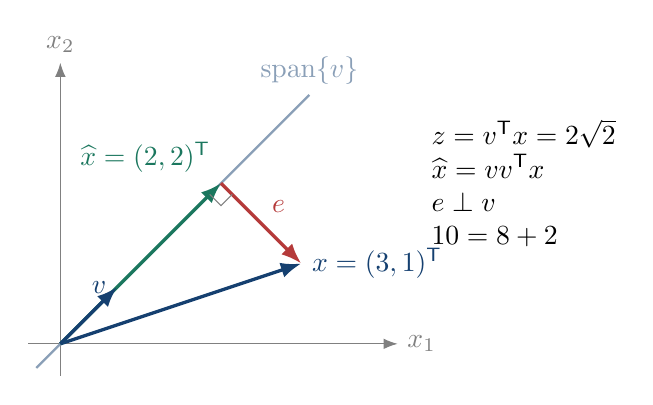
\begin{tikzpicture}[scale=1.02]
\draw[eje](-.4,0)--(4.2,0)node[right]{$x_1$};\draw[eje](0,-.4)--(0,3.5)node[above]{$x_2$};
\draw[azul!50,thick](-.3,-.3)--(3.1,3.1)node[above]{$\spanop\{v\}$};
\draw[vec](0,0)--(3,1)node[right]{$x=(3,1)\T$};
\draw[vecverde](0,0)--(2,2)node[above left]{$\widehat x=(2,2)\T$};
\draw[vecrojo](2,2)--(3,1)node[midway,above right]{$e$};
\draw[vec](0,0)--(.707,.707)node[left]{$v$};
\draw[gray](1.86,1.86)--(2,1.72)--(2.14,1.86);
\node[align=left,anchor=west]at(4.5,2){$z=v\T x=2\sqrt2$\\$\widehat x=vv\T x$\\$e\perp v$\\$10=8+2$};
\end{tikzpicture}
\caption{La coordenada $z$ mide cuánto avanzar sobre el eje unitario; el residuo es perpendicular a la recta.}
\end{figure}
\subsection{Cambiar toda la base no reduce dimensión}
Si $V\in\R^{p\times p}$ es ortogonal, $V\T V=VV\T=I_p$. Para $z=V\T x$, $x=Vz$ y $\norm z_2=\norm x_2$. La rotación o reflexión conserva toda la información. La reducción aparece al descartar coordenadas, usando $V_k\T\in\R^{k\times p}$ con $k<p$.

\section{Autovalores y autovectores: definición y cálculo completo}
\begin{definicion}
Para $A\in\R^{p\times p}$, un escalar $\lambda$ es autovalor si existe $v\in\R^{p\times1}\setminus\{0\}$ tal que $Av=\lambda v$. El vector $v$ es un autovector y
\[
E_\lambda=\kerop(A-\lambda I_p)=\{v:(A-\lambda I_p)v=0\}
\]
es el autoespacio asociado, incluyendo el vector cero como elemento del subespacio.
\end{definicion}
La igualdad significa que $Av$ permanece en la recta de $v$. Si $\lambda>1$, estira; si $0<\lambda<1$, contrae; si $\lambda<0$, invierte el sentido; si $\lambda=0$, anula la dirección. El vector cero no define una dirección y por eso no se llama autovector.
\subsection{Por qué aparece el determinante}
El sistema homogéneo $(A-\lambda I_p)v=0$ tiene solución no nula exactamente cuando su matriz es singular:
\[
\boxed{\det(A-\lambda I_p)=0.}
\]
Se calculan primero las raíces y luego cada núcleo; el determinante no proporciona por sí solo los autovectores. Multiplicar un autovector por cualquier escalar no nulo produce otro; su longitud se fija normalizando y su signo permanece convencional.
\begin{ejemplo}[Resolución exacta de una matriz simétrica]
Para $A=\begin{psmallmatrix}3&1\\1&3\end{psmallmatrix}\in\R^{2\times2}$,
\[
\det(A-\lambda I_2)=(3-\lambda)^2-1=\lambda^2-6\lambda+8
=(\lambda-4)(\lambda-2).
\]
Para $\lambda_1=4$, $-v_1+v_2=0$, luego tomamos $(1,1)\T$ y normalizamos. Para $\lambda_2=2$, $v_1+v_2=0$, luego tomamos $(1,-1)\T$:
\[
v_1=\frac1{\sqrt2}(1,1)\T,\quad v_2=\frac1{\sqrt2}(1,-1)\T,\quad
V=\frac1{\sqrt2}\begin{pmatrix}1&1\\1&-1\end{pmatrix},\quad
\Lambda=\begin{pmatrix}4&0\\0&2\end{pmatrix}.
\]
Ambos $v_j\in\R^{2\times1}$; $V,\Lambda\in\R^{2\times2}$; $V\T V=I_2$. Finalmente,
\[
AV=[Av_1\ Av_2]=[4v_1\ 2v_2]=V\Lambda,
\quad A=V\Lambda V\T=4v_1v_1\T+2v_2v_2\T.
\]
\end{ejemplo}
\subsection{Multiplicidad y casos donde la diagonalización falla}
La multiplicidad algebraica cuenta cuántas veces aparece una raíz del polinomio característico; la geométrica es $\dim E_\lambda$. Una matriz es diagonalizable si admite $p$ autovectores linealmente independientes.
\[
J=\begin{pmatrix}1&1\\0&1\end{pmatrix}:\quad
\det(J-\lambda I_2)=(1-\lambda)^2,\quad E_1=\spanop\{(1,0)\T\}.
\]
Tiene multiplicidad algebraica dos y geométrica uno; no es diagonalizable. En cambio, $A=3I_2$ tiene un solo autovalor distinto, pero \emph{toda} base ortonormal es una base de autovectores. Autovalores repetidos no implican fracaso.
\begin{cuidado}[Simetría no es un adorno]
Una matriz real puede no tener autovectores reales: la rotación $R=\begin{psmallmatrix}0&-1\\1&0\end{psmallmatrix}$ cumple $\lambda^2+1=0$. Su diagonalización requiere $\mathbb C$. Para covarianzas reales, la simetría elimina estas dificultades y garantiza una base ortonormal real.
\end{cuidado}

\section{Teorema espectral real: demostración desde la esfera}
\begin{teorema}[Teorema espectral]
Si $A=A\T\in\R^{p\times p}$, existen una matriz ortogonal $V=[v_1\ \cdots\ v_p]\in\R^{p\times p}$ y una diagonal real $\Lambda=\diag(\lambda_1,\ldots,\lambda_p)$ tales que
\[
\boxed{A=V\Lambda V\T=\sum_{j=1}^p\lambda_jv_jv_j\T},\qquad
Av_j=\lambda_jv_j,\qquad v_i\T v_j=\delta_{ij}.
\]
\end{teorema}
\begin{deduccion}
\textbf{1. Existe una dirección extrema.} La esfera $\Sph^{p-1}=\{v\in\R^{p\times1}:v\T v=1\}$ es compacta y $f(v)=v\T Av$ es continua; por tanto tiene máximo en algún $v_1$. Para cualquier $h\perp v_1$, $h\in\R^{p\times1}$, considera
\[
g(t)=\frac{(v_1+th)\T A(v_1+th)}{\norm{v_1+th}_2^2}.
\]
Como $t=0$ maximiza localmente, $g'(0)=2h\T Av_1=0$. Esto vale para todo $h\perp v_1$, por lo que $Av_1$ es paralelo a $v_1$: $Av_1=\lambda_1v_1$, con $\lambda_1=v_1\T Av_1\in\R$.

\textbf{2. El complemento ortogonal es invariante.} Si $u\in\R^{p\times1}$ y $v_1\T u=0$, entonces
\[
v_1\T Au=(Av_1)\T u=\lambda_1v_1\T u=0.
\]
Así, $A$ envía $v_1^\perp$ a sí mismo. En cualquier base ortonormal de ese subespacio de dimensión $p-1$, su restricción sigue siendo simétrica.

\textbf{3. Inducción.} El caso $p=1$ es inmediato. Aplicando el mismo argumento a la restricción obtenemos $p-1$ autovectores ortonormales dentro de $v_1^\perp$. Junto con $v_1$ forman la base requerida. De $AV=V\Lambda$ y $VV\T=I_p$ se deduce $A=V\Lambda V\T$.
\end{deduccion}
\subsection{Ortogonalidad para autovalores distintos}
Si $Av_i=\lambda_iv_i$ y $Av_j=\lambda_jv_j$,
\[
\lambda_i v_i\T v_j=(Av_i)\T v_j=v_i\T Av_j
=\lambda_jv_i\T v_j
\quad\Rightarrow\quad(\lambda_i-\lambda_j)v_i\T v_j=0.
\]
Si $\lambda_i\ne\lambda_j$, $v_i\T v_j=0$. Dentro de un autoespacio repetido, Gram--Schmidt produce una base ortonormal sin salir del autoespacio.
\subsection{Consecuencias que usaremos continuamente}
Para $a=V\T x\in\R^{p\times1}$ y $x\in\R^{p\times1}$,
\[
x\T Ax=a\T\Lambda a=\sum_j\lambda_ja_j^2,\quad
\tr A=\sum_j\lambda_j,\quad \det A=\prod_j\lambda_j,\quad
\rank A=\#\{j:\lambda_j\ne0\}.
\]
$A$ es semidefinida positiva, escrito $A\succeq0$, si $x\T Ax\ge0$ para todo $x$; equivale a $\lambda_j\ge0$ para todos los $j$. Es definida positiva, $A\succ0$, si todos son estrictamente positivos.
\[
A^{-1}=V\diag(\lambda_j^{-1})V\T\quad(\lambda_j\ne0),\qquad
A^{1/2}=V\diag(\sqrt{\lambda_j})V\T\quad(A\succeq0).
\]
Estas expresiones se comprueban multiplicando y cancelando $V\T V$. La raíz escrita es la única raíz simétrica semidefinida positiva; no se afirma que toda raíz matricial sea única.
\begin{idea}[Lectura geométrica de la descomposición]
$A x=V\Lambda(V\T x)$: primero expresar $x$ en los ejes propios, después escalar cada coordenada por su autovalor y finalmente volver a las coordenadas originales. En esos ejes desaparecen los términos cruzados de la forma cuadrática.
\end{idea}

\section{Cociente de Rayleigh, extremos y varias direcciones}
Para $A=A\T\in\R^{p\times p}$ y $v\ne0$, el cociente de Rayleigh es
\[
\mathcal R_A(v)=\frac{v\T Av}{v\T v}.
\]
Sean $\lambda_1\ge\cdots\ge\lambda_p$ y $a=V\T v\in\R^{p\times1}$. Entonces
\[
\mathcal R_A(v)=\frac{\sum_j\lambda_ja_j^2}{\sum_j a_j^2}
=\sum_j\lambda_j\omega_j,\qquad \omega_j=\frac{a_j^2}{\sum_\ell a_\ell^2},\quad
\omega_j\ge0,\quad\sum_j\omega_j=1.
\]
Es una media ponderada de autovalores; por ello $\lambda_p\le\mathcal R_A(v)\le\lambda_1$. Los extremos se alcanzan en los autoespacios extremos. Así se prueba la optimalidad global, algo que las condiciones de Lagrange por sí solas no garantizan.
\subsection{Lagrange explicado coordenada por coordenada}
Para maximizar $v\T Av$ con $v\T v=1$,
\[
\mathcal L(v,\lambda)=v\T Av-\lambda(v\T v-1),\quad
\frac{\partial\mathcal L}{\partial v_i}=2\sum_ja_{ij}v_j-2\lambda v_i=0.
\]
Agrupar las $p$ ecuaciones da $Av=\lambda v$; premultiplicar por $v\T$ da $\lambda=v\T Av$. Todos los autovectores unitarios son estacionarios, pero solo los del mayor autovalor maximizan.
\subsection{Principio variacional de varias direcciones}
\begin{teorema}[Máxima traza o principio de Ky Fan]
Si $W\in\R^{p\times k}$ y $W\T W=I_k$, entonces
\[
\tr(W\T AW)\le\sum_{j=1}^k\lambda_j,
\qquad\max_{W\T W=I_k}\tr(W\T AW)=\sum_{j=1}^k\lambda_j.
\]
\end{teorema}
\begin{deduccion}
Escribe $B=V\T W\in\R^{p\times k}$, de modo que $B\T B=I_k$. Definimos $h_j=\sum_{\ell=1}^k b_{j\ell}^2=(BB\T)_{jj}$. Como $BB\T$ es proyector, $0\le h_j\le1$ y $\sum_jh_j=k$. Por tanto,
\[
\tr(W\T AW)=\sum_j\lambda_jh_j,
\]
\[
\sum_{j=1}^k\lambda_j-\sum_j\lambda_jh_j
=\sum_{j\le k}\lambda_j(1-h_j)-\sum_{j>k}\lambda_jh_j
\ge\lambda_k\left[\sum_{j\le k}(1-h_j)-\sum_{j>k}h_j\right]=0.
\]
La igualdad se alcanza con $W=V_k=[v_1\ \cdots\ v_k]$. Si $\lambda_k>\lambda_{k+1}$, el subespacio óptimo es único; sus bases ortonormales no lo son.
\end{deduccion}
\subsection{Courant--Fischer: la formulación min--max}
Para $1\le j\le p$,
\[
\lambda_j=\max_{\dim M=j}\ \min_{\substack{v\in M\\\norm v_2=1}}v\T Av
=\min_{\dim N=p-j+1}\ \max_{\substack{v\in N\\\norm v_2=1}}v\T Av.
\]
\textbf{Demostración de la primera igualdad.} Todo $M$ de dimensión $j$ intersecta no trivialmente $\spanop\{v_j,\ldots,v_p\}$ porque las dimensiones suman $p+1$. Un vector unitario de esa intersección tiene cociente a lo sumo $\lambda_j$, así que el mínimo en $M$ no puede superarlo. Para $M=\spanop\{v_1,\ldots,v_j\}$, el mínimo vale $\lambda_j$. La segunda igualdad se demuestra intercambiando los subespacios extremos. Esto conecta una lista de raíces algebraicas con problemas geométricos de optimización.

\parte{IV. Probabilidad vectorial: matrices de momentos y normal multivariada}
\section{Vectores aleatorios y cada entrada de una covarianza}
Un vector aleatorio $\xi=(\xi_1,\ldots,\xi_p)\T$ agrupa $p$ variables definidas sobre el mismo experimento. Su media es $\mu=(\E\xi_1,\ldots,\E\xi_p)\T$, si cada componente es integrable. Con segundos momentos finitos,
\[
\Sigma=\Cov(\xi)=\E[(\xi-\mu)(\xi-\mu)\T]
=\E(\xi\xi\T)-\mu\mu\T\in\R^{p\times p}.
\]
La entrada $ij$ es $\Sigma_{ij}=\Cov(\xi_i,\xi_j)$; la diagonal contiene varianzas. La matriz $\mu\mu\T$ es un producto exterior: no es el escalar $\mu\T\mu$. Las covarianzas pueden ser negativas, pero la matriz completa nunca tiene energía negativa:
\[
a\T\Sigma a=\E[(a\T(\xi-\mu))^2]=\Var(a\T\xi)\ge0.
\]
Así, $\Sigma$ es simétrica semidefinida positiva. Puede ser singular aunque cada componente tenga varianza positiva: si $\xi_2=2\xi_1$, ambas varían pero una combinación se anula.
\subsection{Covarianza cruzada y dimensiones compatibles}
Para $\eta\in\R^q$ con media $\nu$, definimos
\[
C=\Cov(\xi,\eta)=\E[(\xi-\mu)(\eta-\nu)\T]\in\R^{p\times q},
\quad\Cov(\eta,\xi)=C\T.
\]
Si $A\in\R^{m\times p}$, $B\in\R^{s\times q}$, $a\in\R^m$, $b\in\R^s$ son deterministas,
\[
\E(A\xi+a)=A\mu+a,\qquad
\Cov(A\xi+a,B\eta+b)=ACB\T.
\]
En particular $\Cov(A\xi)=A\Sigma A\T$. La prueba es sustituir, restar medias y sacar las matrices deterministas de la esperanza. Si $A$ es \emph{aleatoria}, ese paso no es válido sin condicionar o controlar dependencia.
\begin{ejemplo}[Tres variables construidas a partir de dos fuentes]
Sean $U,V$ independientes, centradas, con varianzas $1,4$. Define $\xi=(U,U+V,2U-V)\T=A(U,V)\T$ con
\[
A=\begin{pmatrix}1&0\\1&1\\2&-1\end{pmatrix},\quad
\Sigma=A\begin{pmatrix}1&0\\0&4\end{pmatrix}A\T
=\begin{pmatrix}1&1&2\\1&5&-2\\2&-2&8\end{pmatrix}.
\]
La combinación $-3\xi_1+\xi_2+\xi_3=0$ explica la singularidad. Para $c=(1,1,1)\T$, $c\T\xi=4U$ y $c\T\Sigma c=16$. Sumar solo la diagonal daría $14$ y perdería los términos cruzados.
\end{ejemplo}
\subsection{Ley de covarianza total}
Para cualquier información $\mathcal G$, sean $m=\E(\xi\mid\mathcal G)$ y $V=\Cov(\xi\mid\mathcal G)$. Con momentos finitos,
\[
\boxed{\Cov(\xi)=\E V+\Cov(m)}.
\]
La prueba matricial copia la escalar: $\xi-\mu=(\xi-m)+(m-\mu)$; los dos productos cruzados tienen esperanza cero al condicionar. Si $\xi$ es un estimador, la identidad distingue incertidumbre dada una matriz de diseño de incertidumbre por cambiar esa matriz.
\subsection{Correlación como covarianza estandarizada}
Si $\Sigma_{jj}>0$, $D=\diag(\sqrt{\Sigma_{11}},\ldots,\sqrt{\Sigma_{pp}})$ y $R=D^{-1}\Sigma D^{-1}$. Sus entradas están entre $-1$ y $1$ por Cauchy--Schwarz aplicado a variables centradas. La matriz de correlación tiene diagonal uno y también es semidefinida positiva. No es una tabla de probabilidades ni una colección arbitraria de números entre $-1$ y $1$.

\section{Normal multivariada: construcción, densidad y transformaciones}
\subsection{Primero construir, después escribir una densidad}
Sean $z_1,\ldots,z_r$ normales estándar independientes y $z=(z_1,\ldots,z_r)\T$. Para $B\in\R^{p\times r}$ y $\mu\in\R^p$, definimos
\[
\xi=\mu+Bz,\qquad\E\xi=\mu,\qquad\Cov(\xi)=BB\T=\Sigma.
\]
Esta construcción incluye normales singulares. Equivale a exigir que cada combinación $a\T\xi$ sea normal escalar, permitiendo varianza cero. Para $\Sigma\succ0$ podemos elegir $B=Q\Lambda^{1/2}$, usando el teorema espectral, con $r=p$.
\subsection{Jacobiano y densidad completa}
La densidad conjunta de $z$ es el producto de $p$ densidades normales:
\[
f_z(z)=(2\pi)^{-p/2}\exp(-z\T z/2).
\]
El cambio $z=B^{-1}(x-\mu)$ transforma volúmenes por $|\det B|^{-1}$. Como $\det\Sigma=(\det B)^2$ y $B^{-\mathsf T}B^{-1}=\Sigma^{-1}$,
\[
\boxed{f_\xi(x)=\frac{1}{(2\pi)^{p/2}\det(\Sigma)^{1/2}}
\exp\!\left[-\frac12(x-\mu)\T\Sigma^{-1}(x-\mu)\right]}.
\]
Escribimos $\xi\sim\mathcal N_p(\mu,\Sigma)$. La raíz del determinante mide el cambio de volumen; la forma cuadrática mide distancia al centro en unidades de covarianza. Si $\Sigma$ es singular, esta fórmula con densidad respecto al volumen de $\R^p$ \emph{no existe}: la probabilidad está concentrada en un subespacio afín de dimensión menor.

\begin{figure}[H]\centering
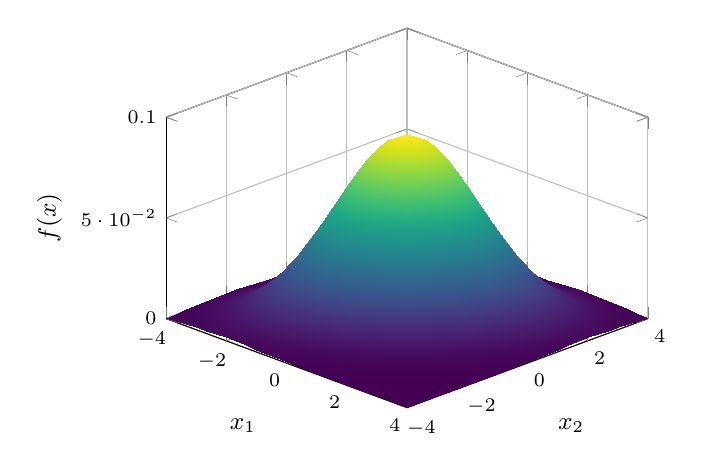
\begin{tikzpicture}\begin{axis}[width=7.7cm,height=6.4cm,view={45}{32},xlabel={$x_1$},ylabel={$x_2$},zlabel={$f(x)$},xmin=-4,xmax=4,ymin=-4,ymax=4,zmin=0,zmax=.1,tick label style={font=\scriptsize},label style={font=\small},grid=major]
\addplot3[surf,shader=interp,domain=-4:4,y domain=-4:4,samples=25,samples y=25,colormap/viridis]{exp(-(x*x-x*y+y*y)/3)/(2*pi*sqrt(3))};
\end{axis}\end{tikzpicture}\hfill
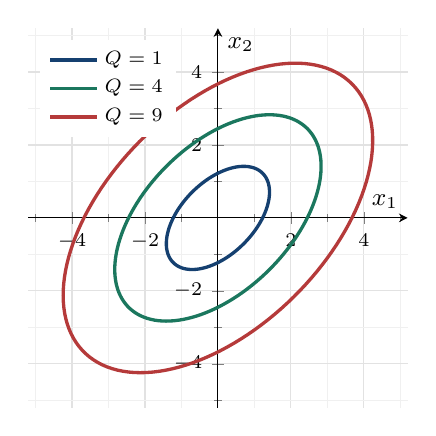
\begin{tikzpicture}\begin{axis}[base,width=7.7cm,height=6.4cm,axis equal image,xmin=-5.2,xmax=5.2,ymin=-5.2,ymax=5.2,xlabel={$x_1$},ylabel={$x_2$},legend pos=north west]
\addplot[azul,very thick,domain=0:360]({(sqrt(3)*cos(x)+sin(x))/sqrt(2)},{(sqrt(3)*cos(x)-sin(x))/sqrt(2)});\addlegendentry{$Q=1$}
\addplot[verde,very thick,domain=0:360]({2*(sqrt(3)*cos(x)+sin(x))/sqrt(2)},{2*(sqrt(3)*cos(x)-sin(x))/sqrt(2)});\addlegendentry{$Q=4$}
\addplot[rojo,very thick,domain=0:360]({3*(sqrt(3)*cos(x)+sin(x))/sqrt(2)},{3*(sqrt(3)*cos(x)-sin(x))/sqrt(2)});\addlegendentry{$Q=9$}
\end{axis}\end{tikzpicture}
\caption{Normal bivariada con media cero y covarianza $\bigl(\begin{smallmatrix}2&1\\1&2\end{smallmatrix}\bigr)$. La superficie representa la densidad; las elipses representan niveles de la distancia cuadrada $Q=x\T\Sigma^{-1}x$, no probabilidades directamente.}
\end{figure}

\subsection{Generadora, independencia y cierre lineal}
Por independencia de las coordenadas de $z$,
\[
M_\xi(t)=\E(e^{t\T\xi})=\exp\!\left(t\T\mu+\frac12t\T\Sigma t\right),
\quad t\in\R^p.
\]
Entonces $A\xi+a\sim\mathcal N_m(A\mu+a,A\Sigma A\T)$ para cualquier matriz determinista $A\in\R^{m\times p}$, aunque el resultado sea singular. Si dividimos $\xi$ en bloques y su covarianza es diagonal por bloques, la generadora se factoriza y esos bloques son independientes. Esta conclusión necesita \emph{normalidad conjunta}, no solo marginales normales.
\begin{cuidado}[Dos normales marginales no garantizan una normal conjunta]
Sea $Z$ normal estándar y $S$ un signo independiente, con probabilidades $1/2$ para $\pm1$. $U=Z$ y $V=SZ$ tienen marginales normales y covarianza $\E S\E Z^2=0$, pero $|U|=|V|$ siempre. Su distribución conjunta vive sobre dos rectas y no son independientes. Una normal conjunta de covarianza $I_2$ tendría densidad positiva en todo $\R^2$.
\end{cuidado}
\subsection{Blanqueamiento, radio y probabilidad elipsoidal}
Si $w=\Sigma^{-1/2}(\xi-\mu)$, $w\sim\mathcal N_p(0,I_p)$. Por tanto,
\[
Q=(\xi-\mu)\T\Sigma^{-1}(\xi-\mu)=w\T w\sim\chi^2_p,
\quad\E Q=p,\quad\Var(Q)=2p.
\]
El conjunto $Q\le c$ tiene probabilidad $\Prob(\chi_p^2\le c)$: un contorno con distancia de Mahalanobis uno no contiene el mismo porcentaje al cambiar $p$. En $p=1000$, el radio típico es del orden de $\sqrt{1000}$, no de uno. Si la normal tiene rango $r<p$ y se restringe a su soporte, la forma con $\Sigma^+$ sigue $\chi^2_r$.
\subsection{Entropía y volumen de incertidumbre}
La entropía diferencial se define como $h(\xi)=-\E\log f_\xi(\xi)$. Insertar la densidad y usar $\E Q=p$ da
\[
h(\xi)=\frac12\log\!\left[(2\pi e)^p\det\Sigma\right].
\]
No es una probabilidad y puede ser negativa. Un cambio lineal invertible $A$ añade $\log|\det A|$ a la entropía, porque cambia las unidades de volumen. La varianza sobre un eje y el volumen total son dos resúmenes distintos de la dispersión.

\section{Normal condicional, complemento de Schur y regresión poblacional}
Particionemos $\xi=(u\T,v\T)\T$ con dimensiones $a,b$, media $(\mu_u\T,\mu_v\T)\T$ y covarianza positiva definida
\[
\Sigma=\begin{pmatrix}A&C\\C\T&D\end{pmatrix},\quad
A\in\R^{a\times a},\ C\in\R^{a\times b},\ D\in\R^{b\times b}.
\]
Definimos el residuo $e=u-\mu_u-CD^{-1}(v-\mu_v)$. Entonces
\[
\E e=0,\quad\Cov(e,v)=C-CD^{-1}D=0,
\quad\Cov(e)=A-CD^{-1}C\T=:S_{u\mid v}.
\]
Como $(e,v)$ es normal conjunta, covarianza cruzada cero implica independencia. Por ello
\[
\boxed{u\mid v\sim\mathcal N_a\!\left(\mu_u+CD^{-1}(v-\mu_v),\ A-CD^{-1}C\T\right)}.
\]
La media condicional es afín y la covarianza condicional no depende del valor observado de $v$. Fuera de la familia normal, una covarianza cruzada conocida no basta para afirmar ninguna de esas dos propiedades.
\subsection{Por qué el complemento de Schur es positivo}
Para $h\in\R^a$, toma $k=-D^{-1}C\T h$. Entonces
\[
\begin{pmatrix}h\\k\end{pmatrix}\T\Sigma\begin{pmatrix}h\\k\end{pmatrix}
=h\T(A-CD^{-1}C\T)h>0\quad(h\ne0).
\]
Además, multiplicar bloques verifica
\[
\Sigma^{-1}=\begin{pmatrix}
S^{-1}&-S^{-1}CD^{-1}\\
-D^{-1}C\T S^{-1}&D^{-1}+D^{-1}C\T S^{-1}CD^{-1}
\end{pmatrix},\quad S=A-CD^{-1}C\T.
\]
Y una eliminación por bloques da $\det\Sigma=\det D\det S$. Estas identidades explican simultáneamente condicionamiento gaussiano, eliminación de parámetros y cómputo de modelos de factores.
\begin{ejemplo}[Predecir una variable con otra y cuantificar el residuo]
\[
\begin{pmatrix}U\\V\end{pmatrix}\sim\mathcal N_2\!\left(
\begin{pmatrix}2\\-1\end{pmatrix},
\begin{pmatrix}9&3\\3&4\end{pmatrix}\right).
\]
Entonces $U\mid V=v\sim\mathcal N(2+\tfrac34(v+1),\tfrac{27}4)$. Si observamos $V=3$, la media condicional es $5$ y la varianza $6.75$. La varianza total se verifica como $6.75+(3/4)^2\cdot4=9$. La observación reduce incertidumbre; no la elimina.
\end{ejemplo}
\subsection{Mejor predictor lineal aunque no haya normalidad}
Para variables con momentos finitos, buscamos $\min_{a,B}\E\norm{u-a-Bv}_2^2$. Optimizar $a$ da $a=\mu_u-B\mu_v$. Al expandir la pérdida y derivar respecto a $B$ obtenemos $BD=C$, así que $B=CD^{-1}$. El residuo queda incorrelacionado con $v$. Este resultado describe el mejor predictor \emph{lineal}; la esperanza condicional podría ser no lineal.

\section{Cuartos momentos, formas cuadráticas y sus covarianzas}
Si $z\sim\mathcal N_p(0,\Sigma)$, derivamos cuatro veces $M_z(t)=\exp(t\T\Sigma t/2)$ y evaluamos en cero. Cada término no nulo empareja dos índices:
\[
\boxed{\E[z_iz_jz_kz_\ell]=
\Sigma_{ij}\Sigma_{k\ell}+\Sigma_{ik}\Sigma_{j\ell}+\Sigma_{i\ell}\Sigma_{jk}}.
\]
Todos los momentos impares centrados son cero porque la distribución es simétrica bajo $z\mapsto-z$. La fórmula anterior generaliza $\E Z^4=3$ y permite calcular covarianzas de productos sin suponer que los productos sean independientes.
\subsection{Una forma cuadrática: esperanza entrada por entrada}
Para $x$ de media $\mu$ y covarianza $\Sigma$, y $A\in\R^{p\times p}$ determinista,
\begin{align*}
\E(x\T Ax)&=\sum_{i,j}a_{ij}\E(x_ix_j)
=\sum_{i,j}a_{ij}(\Sigma_{ij}+\mu_i\mu_j)\\
&=\tr(A\Sigma)+\mu\T A\mu.
\end{align*}
No exige normalidad. Solo importa la parte simétrica de $A$, pues $x\T(A-A\T)x=0$. Si $x$ es normal y $A,B$ son simétricas, la fórmula de cuatro momentos da
\[
\Cov(x\T Ax,x\T Bx)=2\tr(A\Sigma B\Sigma)+4\mu\T A\Sigma B\mu,
\]
\[
\boxed{\Var(x\T Ax)=2\tr[(A\Sigma)^2]+4\mu\T A\Sigma A\mu}.
\]
\begin{deduccion}
Escribe $x=\mu+z$. La parte aleatoria es $2\mu\T Az+z\T Az$. El término lineal tiene varianza $4\mu\T A\Sigma A\mu$. Su covarianza con el cuadrático es cero por momentos impares. Al expandir $\E[(z\T Az)(z\T Bz)]$, el primer emparejamiento produce $\tr(A\Sigma)\tr(B\Sigma)$ y se cancela al centrar; los otros dos producen $2\tr(A\Sigma B\Sigma)$.
\end{deduccion}
\subsection{Distribución de la energía, no solo sus momentos}
Para $z\sim\mathcal N_p(0,I_p)$ y $A=Q\diag(a_1,\ldots,a_p)Q\T$,
\[
z\T Az=\sum_j a_jW_j^2,
\quad W=Q\T z\sim\mathcal N_p(0,I_p).
\]
Por tanto es una suma ponderada de chi-cuadrados independientes. Si $A$ es una proyección de rango $r$, sus autovalores son $r$ unos y el resto ceros, y $z\T Az\sim\chi^2_r$. Si hay autovalores negativos, la forma cuadrática puede ser negativa y no sigue una chi-cuadrado ordinaria.
\begin{ejemplo}[Una forma en mil dimensiones con rango veinte]
Sea $P=P\T=P^2\in\R^{1000\times1000}$ con rango $20$. Para $z$ normal estándar de dimensión $1000$, $z\T Pz\sim\chi^2_{20}$, con esperanza $20$ y varianza $40$. El tamaño de la matriz es $1000$, pero los grados de libertad los determina el rango $20$.
\end{ejemplo}

\section{Media y covarianza muestrales: exactitud, Wishart y matriz de precisión}
Sean $x_1,\ldots,x_n$ independientes con la misma media $\mu$ y covarianza $\Sigma$, $n\ge2$. Definimos
\[
\bar x=\frac1n\sum_i x_i,\qquad
S=\frac1{n-1}\sum_i(x_i-\bar x)(x_i-\bar x)\T.
\]
Por linealidad e independencia, $\E\bar x=\mu$, $\Cov(\bar x)=\Sigma/n$. El desarrollo
\[
(n-1)S=\sum_i(x_i-\mu)(x_i-\mu)\T-n(\bar x-\mu)(\bar x-\mu)\T
\]
da $\E S=\Sigma$. Este es un resultado exacto para cualquier distribución con segundos momentos, no solo la normal.
\subsection{Rotar observaciones separa media y residuos gaussianos}
Ahora supón $x_i\sim\mathcal N_p(\mu,\Sigma)$ con $\Sigma\succ0$. Apila $(x_i-\mu)\T$ en una matriz $D\in\R^{n\times p}$. Elige una matriz ortogonal $O\in\R^{n\times n}$ cuya primera fila sea $\ones_n\T/\sqrt n$. Las filas de $OD$ son normales conjuntas con covarianza cruzada cero porque las filas de $O$ son ortogonales. Son, por tanto, independientes, cada una con covarianza $\Sigma$.
La primera fila es $\sqrt n(\bar x-\mu)\T$; las restantes $n-1$ filas, llamadas $w_a\T$, generan toda la energía residual:
\[
\bar x\sim\mathcal N_p(\mu,\Sigma/n),\quad
(n-1)S=\sum_{a=1}^{n-1}w_aw_a\T,
\quad\bar x\ \text{independiente de }S.
\]
La última suma define la distribución Wishart $W_p(\Sigma,\nu)$ con $\nu=n-1$. Esta definición también sirve cuando la matriz es singular: su rango no supera $\nu$.
\subsection{Esperanza y covarianza de todas las entradas}
Cada $w_a$ tiene $\E(w_{ai}w_{aj})=\Sigma_{ij}$. Los cuartos momentos dan
\[
\Cov(w_{ai}w_{aj},w_{ak}w_{a\ell})
=\Sigma_{ik}\Sigma_{j\ell}+\Sigma_{i\ell}\Sigma_{jk}.
\]
Como sumamos $n-1$ vectores independientes y dividimos por $(n-1)^2$,
\[
\boxed{\Cov(S_{ij},S_{k\ell})=
\frac{\Sigma_{ik}\Sigma_{j\ell}+\Sigma_{i\ell}\Sigma_{jk}}{n-1}}.
\]
En particular,
\[
\Var(S_{ii})=\frac{2\Sigma_{ii}^2}{n-1},\quad
\Var(S_{ij})=\frac{\Sigma_{ii}\Sigma_{jj}+\Sigma_{ij}^2}{n-1},\quad
\Cov(S_{ii},S_{jj})=\frac{2\Sigma_{ij}^2}{n-1}.
\]
Son fórmulas exactas bajo normalidad. Sin normalidad aparecen cuartos momentos adicionales, y si estos no son finitos la varianza de $S$ puede ser infinita aunque $\Sigma$ exista.
\subsection{Forma vectorizada y simetría}
La operación $\operatorname{vec}$ apila columnas de una matriz. Sea $K_{pp}$ la matriz que cumple $K_{pp}\operatorname{vec}(A)=\operatorname{vec}(A\T)$, y $\otimes$ el producto de Kronecker. La misma fórmula de entradas se resume como
\[
\Cov(\operatorname{vec}S)=\frac1{n-1}(I_{p^2}+K_{pp})(\Sigma\otimes\Sigma).
\]
Es una matriz de tamaño $p^2\times p^2$, singular por la duplicación de entradas simétricas. Esta expresión es una identidad teórica; en $p=1000$ no conviene formar sus $10^{12}$ entradas.
\subsection{Invertir una estimación insesgada crea sesgo}
Para $W\sim W_p(\Sigma,\nu)$, $\nu>p+1$,
\[
\E W^{-1}=\frac{\Sigma^{-1}}{\nu-p-1},\qquad
\boxed{\E S^{-1}=\frac{n-1}{n-p-2}\Sigma^{-1}\quad(n>p+2)}.
\]
Una deducción usa la densidad Wishart, proporcional a $\det(W)^{(\nu-p-1)/2}e^{-\tr(\Sigma^{-1}W)/2}$ en matrices positivas definidas. Integrar una derivada respecto a una entrada diagonal da
\[
0=\frac{\nu-p-1}2\E[(W^{-1})_{jj}]-\frac12(\Sigma^{-1})_{jj}.
\]
Para una entrada libre fuera de la diagonal, simetría duplica ambas derivadas y se obtiene la misma relación. Las condiciones de integrabilidad y desaparición del término de frontera exigen $\nu>p+1$. La constante de normalización se cancela; esta deducción presupone la densidad Wishart indicada, cuya construcción por suma ya dimos.
Si $n\le p$, $S$ es singular por rango; si $n=p+1$ o $p+2$, puede ser invertible casi seguramente y aun así $\E S^{-1}$ no ser finita. Existencia de una inversa observada y existencia de su esperanza son cuestiones distintas.
\begin{ejemplo}[El sesgo de precisión puede ser enorme]
En $p=20$, $n=30$, el factor es $29/8=3.625$. Una covarianza muestral insesgada produce una inversa con esperanza $3.625\Sigma^{-1}$. En $p=1000$, $n=200$, ni siquiera existe la inversa ordinaria. La regularización modifica el problema estadístico, no solo la implementación.
\end{ejemplo}

\section{Normal multivariada frente a Student y mezclas gaussianas}
Sean $z\sim\mathcal N_p(0,\Sigma)$ y $Q\sim\chi^2_\nu$ independientes. Definimos
\[
x=\mu+\frac{z}{\sqrt{Q/\nu}}.
\]
Condicionalmente a $Q=q$, $x$ es normal con covarianza $\nu\Sigma/q$. Integrando esa densidad contra la gamma de $Q$,
\[
f_x(x)=\frac{\Gamma((\nu+p)/2)}{\Gamma(\nu/2)(\nu\pi)^{p/2}\det\Sigma^{1/2}}
\left[1+\frac{(x-\mu)\T\Sigma^{-1}(x-\mu)}\nu\right]^{-(\nu+p)/2}.
\]
Para $\nu>1$, $\E x=\mu$; para $\nu>2$, $\Cov(x)=\nu\Sigma/(\nu-2)$. Aquí $\Sigma$ es una \emph{matriz de escala}; no coincide con la covarianza salvo en el límite normal. Toda combinación lineal tiene una Student escalar con los mismos grados de libertad y escala correspondiente.
\subsection{Una escala común introduce dependencia}
Si $\Sigma=I_p$, dos coordenadas tienen covarianza cero, pero comparten el denominador. Para $\nu>4$,
\[
\Cov((x_1-\mu_1)^2,(x_2-\mu_2)^2)
=\frac{2\nu^2}{(\nu-2)^2(\nu-4)}>0.
\]
En efecto $\E(Q^{-2})=1/[(\nu-2)(\nu-4)]$ y $\E(Q^{-1})=1/(\nu-2)$. La incertidumbre en una escala oculta genera movimientos conjuntos de magnitud aunque no exista correlación lineal.
\subsection{Mezclas: separar variación interna y entre centros}
Si $G$ toma valores $1,\ldots,m$ con probabilidades $\pi_g$, y $x\mid G=g\sim\mathcal N_p(\mu_g,\Sigma_g)$, entonces
\[
\mu=\sum_g\pi_g\mu_g,\quad
\Cov(x)=\sum_g\pi_g\Sigma_g+
\sum_g\pi_g(\mu_g-\mu)(\mu_g-\mu)\T.
\]
La mezcla generalmente no es normal. Una dirección principal puede representar diferencias entre grupos en vez de ruido dentro de cada grupo. Conocer media y covarianza no identifica toda una distribución fuera de una familia paramétrica especificada.

\parte{V. Cálculo vectorial y matricial: derivar antes de optimizar}
\section{Diferencial, gradiente, Jacobiano y Hessiana: cuatro objetos}
Sea $f:\R^p\to\R$. Su diferencial en $x$ es la aplicación lineal que aproxima el incremento:
\[
f(x+h)=f(x)+\mathrm df_x[h]+o(\norm h_2),\qquad
\mathrm df_x[h]=\nabla f(x)\T h.
\]
El símbolo $o(\norm h)$ significa un resto cuyo cociente por $\norm h$ tiende a cero. El gradiente $\nabla f(x)\in\R^p$ representa ese funcional con el producto euclidiano; su coordenada $j$ es $\partial f/\partial x_j$. Para $F:\R^p\to\R^m$, el Jacobiano $J_F(x)\in\R^{m\times p}$ contiene $\partial F_i/\partial x_j$, y $F(x+h)=F(x)+J_F(x)h+o(\norm h)$.
Si $f$ admite segundas derivadas continuas, la Hessiana $H_f(x)$ es la matriz $p\times p$ de derivadas cruzadas, y
\[
f(x+h)=f(x)+\nabla f(x)\T h+\frac12h\T H_f(x)h+o(\norm h_2^2).
\]
No hay cuatro nombres para lo mismo: la diferencial es una aplicación lineal, el gradiente un vector, el Jacobiano una matriz entre dos espacios y la Hessiana una forma cuadrática de segundo orden.
\subsection{Gradiente bajo otra métrica}
Si usamos $\ip uv_G=u\T Gv$ con $G\succ0$, exigimos $\mathrm df_x[h]=\ip{\nabla_G f(x)}h_G$. Por tanto $G\nabla_G f=\nabla f$ y
\[
\nabla_G f=G^{-1}\nabla f.
\]
El diferencial no cambia; el vector que lo representa sí. Este hecho une precondicionamiento, escalado de variables y direcciones de descenso.
\subsection{Regla de la cadena con dimensiones}
Si $g:\R^m\to\R$ y $F:\R^p\to\R^m$,
\[
\nabla(g\circ F)(x)=J_F(x)\T\nabla g(F(x)).
\]
El producto tiene dimensiones $(p\times m)(m\times1)=p\times1$. Para $F(x)=Ax-b$ y $g(r)=r\T r/2$, $J_F=A$ y $\nabla g=r$, de donde
\[
\nabla_x\frac12\norm{Ax-b}_2^2=A\T(Ax-b),\qquad H=A\T A.
\]
La Hessiana es semidefinida positiva incluso si $A$ es rectangular o singular.
\begin{ejemplo}[Un cálculo sin notación abreviada]
Para $f(s,t)=\tfrac12[(s+2t-1)^2+(3s-t-2)^2]$,
\[
\nabla f=\begin{pmatrix}10s-t-7\\-s+5t\end{pmatrix},\quad
H_f=\begin{pmatrix}10&-1\\-1&5\end{pmatrix}.
\]
Resolver $\nabla f=0$ da $t=1/7$, $s=5/7$. El determinante de la Hessiana es $49>0$ y su primera diagonal es positiva; el mínimo es único. La formulación matricial obtiene el mismo resultado con $A=\begin{psmallmatrix}1&2\\3&-1\end{psmallmatrix}$, $b=(1,2)\T$.
\end{ejemplo}

\section{Diferenciales matriciales: producto, inversa, traza y determinante}
Para $f:\R^{m\times p}\to\R$ definimos el gradiente $\nabla_A f$ por
\[
\mathrm df=\tr[(\nabla_A f)\T\mathrm dA]
=\sum_{i,j}\frac{\partial f}{\partial a_{ij}}\mathrm da_{ij}.
\]
La traza evita perder transpuestas. No se deriva una matriz ``como si fuera un escalar'' cuando el orden de los productos importa.
\subsection{Producto e inversa por diferenciación de identidades}
De $(A+\mathrm dA)(B+\mathrm dB)$ y descartando el producto de incrementos, sale $\mathrm d(AB)=(\mathrm dA)B+A\mathrm dB$. Si $A$ es invertible, diferenciar $AA^{-1}=I$ da
\[
(\mathrm dA)A^{-1}+A\mathrm d(A^{-1})=0,
\qquad\boxed{\mathrm d(A^{-1})=-A^{-1}(\mathrm dA)A^{-1}}.
\]
El orden es esencial: $-A^{-2}\mathrm dA$ solo sería válido si los factores conmutaran. Para $f(A)=\tr(C\T A)$, $\nabla_A f=C$. Para $f(A)=\norm A\F^2=\tr(A\T A)$, $\mathrm df=2\tr(A\T\mathrm dA)$ y $\nabla_A f=2A$.
\subsection{Formas cuadráticas de una matriz}
Si $S=S\T$ y $T=T\T$ son constantes compatibles,
\[
f(A)=\tr(A\T SAT),\quad
\mathrm df=\tr[(\mathrm dA)\T SAT]+\tr[A\T S(\mathrm dA)T],
\]
y rotar cíclicamente la segunda traza da $\nabla_A f=2SAT$. Sin simetría la fórmula general es $SAT+S\T AT\T$.
\subsection{Determinante y logaritmo del determinante}
El determinante es una función multilineal alternante de columnas, normalizada por $\det I=1$. Expandir por cofactores produce, para una matriz invertible,
\[
\mathrm d\det A=\det A\,\tr(A^{-1}\mathrm dA).
\]
Si $A\succ0$, $\det A>0$ y
\[
\mathrm d\log\det A=\tr(A^{-1}\mathrm dA),\qquad
\nabla_A\log\det A=A^{-\mathsf T}.
\]
Para un incremento simétrico $H$, la segunda derivada direccional es
\[
\mathrm d^2\log\det A[H,H]=-\tr(A^{-1}HA^{-1}H)
=-\norm{A^{-1/2}HA^{-1/2}}\F^2\le0.
\]
Por ello $-\log\det A$ es convexa sobre matrices positivas definidas. La frontera singular hace que esa barrera tienda a $+\infty$.
\subsection{Vectorizar convierte derivadas de matrices en sistemas lineales}
Si $A\in\R^{a\times b}$, $B\in\R^{b\times c}$, $C\in\R^{c\times d}$,
\[
\operatorname{vec}(ABC)=(C\T\otimes A)\operatorname{vec}B.
\]
La entrada correspondiente a $i,j$ en ambos lados es $\sum_{k,\ell}a_{ik}b_{k\ell}c_{\ell j}$, lo que demuestra la identidad. Así,
\[
\operatorname{vec}(\mathrm dA^{-1})
=-(A^{-\mathsf T}\otimes A^{-1})\operatorname{vec}(\mathrm dA).
\]
Esta matriz Jacobiana permite propagar covarianzas de una covarianza estimada hacia una precisión estimada mediante el método delta, siempre que la matriz poblacional sea invertible y el régimen asintótico lo permita.

\section{Convexidad y mínimos globales: qué garantiza la Hessiana}
Un conjunto $C$ es convexo si $(1-t)x+ty\in C$ para $x,y\in C$, $t\in[0,1]$. Una función convexa cumple
\[
f((1-t)x+ty)\le(1-t)f(x)+tf(y).
\]
Para una función diferenciable en un dominio abierto convexo, una condición equivalente es
\[
f(y)\ge f(x)+\nabla f(x)\T(y-x).
\]
Se obtiene tomando el límite $t\downarrow0$ de la desigualdad de convexidad; la implicación inversa se verifica aplicando esta cota en el punto intermedio a ambos extremos. Si $\nabla f(x_*)=0$, esa desigualdad prueba $f(y)\ge f(x_*)$ para todo $y$: el mínimo es global.
\subsection{Prueba del criterio de segundo orden}
Restrinja $f$ a la recta $g(t)=f(x+th)$. Entonces $g''(t)=h\T H_f(x+th)h$. Si $H_f\succeq0$ en todo el dominio, $g'$ es creciente y $g$ convexa en cada segmento; por ello $f$ es convexa. Si $H_f\succeq mI$ con $m>0$,
\[
f(y)\ge f(x)+\nabla f(x)\T(y-x)+\frac m2\norm{y-x}_2^2.
\]
Esto es convexidad fuerte y asegura unicidad del mínimo cuando existe. Una Hessiana positiva en un único punto estacionario solo prueba un mínimo local; no la convexidad de toda la función.
\subsection{Una cuadrática completa por completar cuadrados}
Para $Q=Q\T\succ0$,
\[
f(x)=\frac12x\T Qx-c\T x+d,
\quad x_*=Q^{-1}c,
\quad f(x)=f(x_*)+\frac12(x-x_*)\T Q(x-x_*).
\]
Si $Q\succeq0$ es singular y $c\notin\range Q$, existe $h\in\kerop Q$ con $c\T h\ne0$, y $f(th)$ desciende sin cota en un sentido. Si $c\in\range Q$, hay mínimos $Q^+c+\kerop Q$. Singularidad no significa siempre ``no hay solución'': puede significar falta de unicidad.
\subsection{Descenso por gradiente y condición espectral}
Para la cuadrática positiva definida, la actualización $x_{k+1}=x_k-\alpha(Qx_k-c)$ da
\[
e_{k+1}=(I-\alpha Q)e_k,\quad e_k=x_k-x_*.
\]
En cada autovector, el error se multiplica por $1-\alpha\lambda_j$. Converge desde todo inicio si $0<\alpha<2/\lambda_{\max}$. La elección óptima entre pasos constantes es
\[
\alpha_*=\frac2{\lambda_{\max}+\lambda_{\min}},\quad
\rho_*=\frac{\kappa-1}{\kappa+1},\quad
\kappa=\lambda_{\max}/\lambda_{\min}.
\]
Un problema mal condicionado tiene $\rho_*$ cerca de uno. Newton usa $x_{k+1}=x_k-H_f(x_k)^{-1}\nabla f(x_k)$ y resuelve una cuadrática en un paso en aritmética exacta. En código se resuelve el sistema para el paso; no es necesario construir una inversa explícita.
\begin{figure}[H]\centering
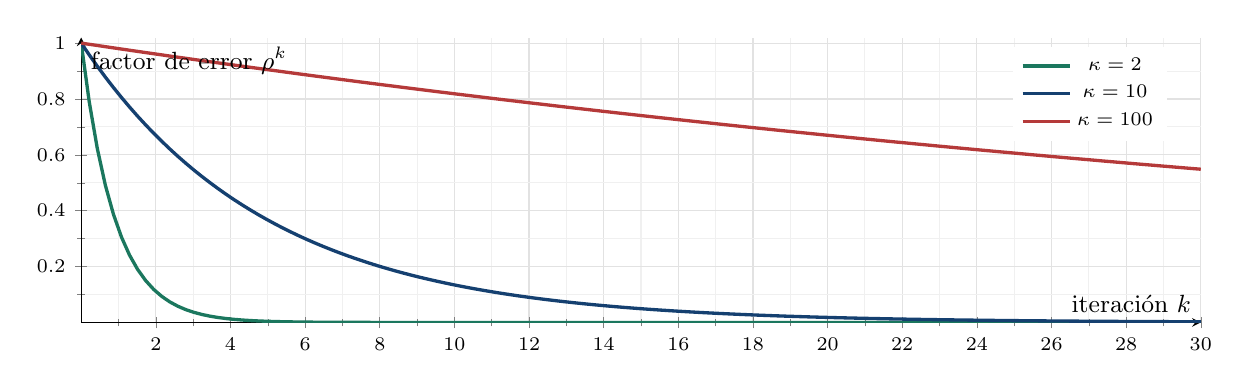
\begin{tikzpicture}\begin{axis}[base,width=15.8cm,height=5.2cm,xlabel={iteración $k$},ylabel={factor de error $\rho^k$},xmin=0,xmax=30,ymin=0,ymax=1.02,legend pos=north east]
\addplot[verde,very thick,domain=0:30]{(1/3)^x};\addlegendentry{$\kappa=2$}
\addplot[azul,very thick,domain=0:30]{(9/11)^x};\addlegendentry{$\kappa=10$}
\addplot[rojo,very thick,domain=0:30]{(99/101)^x};\addlegendentry{$\kappa=100$}
\end{axis}\end{tikzpicture}
\caption{Contracción espectral con el mejor paso constante para una cuadrática. Una covarianza mal condicionada puede dificultar tanto optimización como inferencia.}
\end{figure}

\section{Restricciones lineales, Lagrange y condiciones KKT}
Considera $\min_x\tfrac12x\T Qx-c\T x$ sujeto a $A x=b$, con $Q\succ0$ y $A\in\R^{m\times p}$ de rango fila completo. La Lagrangiana es
\[
\mathcal L(x,\lambda)=\frac12x\T Qx-c\T x+\lambda\T(Ax-b).
\]
Derivar respecto a $x,\lambda$ da el sistema por bloques
\[
\begin{pmatrix}Q&A\T\\A&0\end{pmatrix}
\begin{pmatrix}x\\\lambda\end{pmatrix}
=\begin{pmatrix}c\\b\end{pmatrix}.
\]
Primero $x=Q^{-1}(c-A\T\lambda)$ y luego
\[
\lambda=(AQ^{-1}A\T)^{-1}(AQ^{-1}c-b),\quad
x=Q^{-1}c-Q^{-1}A\T(AQ^{-1}A\T)^{-1}(AQ^{-1}c-b).
\]
La inversa central existe porque $A$ tiene rango fila completo. Para comprobar mínimo global, sea $h$ cualquier perturbación factible, $Ah=0$:
\[
f(x+h)-f(x)=h\T(Qx-c)+\frac12h\T Qh
=-h\T A\T\lambda+\frac12h\T Qh\ge0.
\]
Esto deduce suficiencia sin confiar solo en que las derivadas se anulan.

\begin{figure}[H]\centering
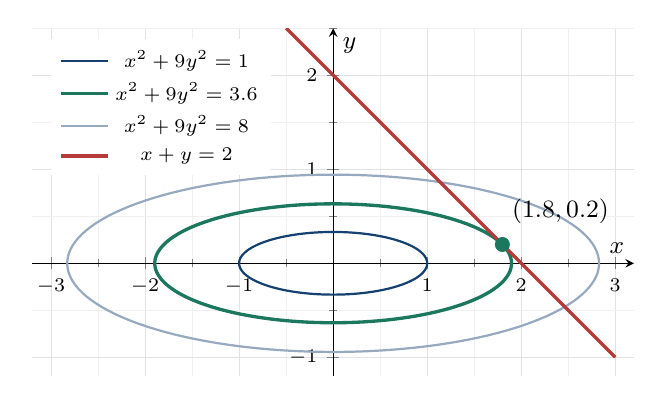
\begin{tikzpicture}\begin{axis}[base,width=15.8cm,height=6cm,axis equal image,xmin=-3.2,xmax=3.2,ymin=-1.2,ymax=2.5,xlabel={$x$},ylabel={$y$},legend pos=north west]
\addplot[azul,domain=0:360,thick]({cos(x)},{sin(x)/3});\addlegendentry{$x^2+9y^2=1$}
\addplot[verde,domain=0:360,very thick]({sqrt(3.6)*cos(x)},{sqrt(3.6)*sin(x)/3});\addlegendentry{$x^2+9y^2=3.6$}
\addplot[azul!45,domain=0:360,thick]({sqrt(8)*cos(x)},{sqrt(8)*sin(x)/3});\addlegendentry{$x^2+9y^2=8$}
\addplot[rojo,very thick,domain=-.5:3]{2-x};\addlegendentry{$x+y=2$}
\addplot[only marks,mark=*,mark size=2.5pt,verde]coordinates{(1.8,.2)};
\node[font=\small,anchor=west]at(axis cs:1.8,.55){$(1.8,0.2)$};
\end{axis}\end{tikzpicture}
\caption{Minimizar $\tfrac12(x^2+9y^2)$ sujeto a $x+y=2$. Lagrange da $x=9y$, y la solución es $(1.8,0.2)$. La curva de nivel mínima factible es tangente a la recta.}
\end{figure}

\subsection{Desigualdades y complementariedad}
Para minimizar una función convexa $f$ con $g_j(x)\le0$ convexas y $Ax=b$, introducimos $\alpha_j\ge0$:
\[
\mathcal L=f(x)+\sum_j\alpha_jg_j(x)+\lambda\T(Ax-b).
\]
Las condiciones KKT son factibilidad primal, factibilidad dual, estacionariedad y complementariedad:
\[
g_j(x)\le0,\quad Ax=b,\quad\alpha_j\ge0,\quad
\nabla f+\sum_j\alpha_j\nabla g_j+A\T\lambda=0,\quad\alpha_jg_j(x)=0.
\]
Una restricción estrictamente inactiva tiene multiplicador cero. En problemas convexos estas condiciones son suficientes: por convexidad, el punto minimiza la Lagrangiana, y complementariedad hace coincidir objetivo y Lagrangiana en él. Para que sean además necesarias se requiere una cualificación de restricciones; la existencia de un punto estrictamente factible para las desigualdades, llamado condición de Slater, es una condición suficiente habitual. No se usa KKT como necesidad universal sin hipótesis.
\subsection{Dualidad: por qué una minimización genera una maximización}
La función dual $g(\lambda,\alpha)=\inf_x\mathcal L(x,\lambda,\alpha)$ es una cota inferior al mínimo primal para $\alpha\ge0$. En efecto, en un punto factible $\mathcal L(x,\lambda,\alpha)\le f(x)$. Maximizar la cota inferior busca la mejor certificación posible. En convexidad con Slater, el valor dual coincide con el primal; en SVR construiremos ambas expresiones y verificaremos KKT para ejemplos concretos.

\section{No diferenciabilidad: subgradientes y regularización dispersa}
Un subgradiente de $f$ convexa en $x$ es un vector $s$ con $f(y)\ge f(x)+s\T(y-x)$ para todo $y$. Para $f(t)=|t|$,
\[
\partial|t|=\{1\}\ (t>0),\quad\{-1\}\ (t<0),\quad[-1,1]\ (t=0).
\]
La función $|t|$ no tiene derivada en cero, pero sí muchos subgradientes. Un punto minimiza una función convexa si y solo si $0\in\partial f(x)$: la definición prueba ambas direcciones.
\subsection{Umbral suave deducido por casos}
Para $\lambda\ge0$, resuelve
\[
\min_w\frac12(w-a)^2+\lambda|w|.
\]
Si $w>0$, estacionariedad da $w=a-\lambda$, admisible cuando $a>\lambda$. Si $w<0$, da $w=a+\lambda$ cuando $a<-\lambda$. En $w=0$, la condición es $a\in[-\lambda,\lambda]$. Por tanto,
\[
\boxed{\operatorname{soft}_\lambda(a)=\sign(a)(|a|-\lambda)_+},\qquad (t)_+=\max(t,0).
\]
La solución vectorial con pérdida $\norm{w-a}_2^2/2+\lambda\norm w_1$ se separa por coordenadas. Esa separabilidad desaparece si sustituimos identidad por un diseño general correlacionado.
\subsection{Operador proximal y Lasso}
El proximal de una penalización convexa $h$ es $\operatorname{prox}_{\eta h}(a)=\argmin_w\{\norm{w-a}_2^2/2+\eta h(w)\}$. En Lasso,
\[
\min_\beta\frac12\norm{y-X\beta}_2^2+\lambda\norm\beta_1,
\quad 0\in X\T(X\beta-y)+\lambda\partial\norm\beta_1.
\]
Un paso proximal de gradiente es $\beta^+=\operatorname{soft}_{\eta\lambda}(\beta+\eta X\T(y-X\beta))$, coordenada por coordenada. Ridge usa penalización cuadrática y una solución lineal; Lasso introduce selección de coordenadas y una solución no lineal en $y$. Esa diferencia tendrá consecuencias para sus esperanzas y covarianzas.

\parte{VI. De los datos a PCA: cada matriz y cada optimización}
\section{Datos, centrado y covarianza: dimensiones explícitas}
Las observaciones $x_i\in\R^{p\times1}$ se apilan como \emph{filas}:
\[
X=\begin{pmatrix}x_1\T\\\vdots\\x_n\T\end{pmatrix}
=\begin{pmatrix}x_{11}&\cdots&x_{1p}\\\vdots&\ddots&\vdots\\x_{n1}&\cdots&x_{np}\end{pmatrix}\in\R^{n\times p},\qquad
\bar x=\frac1n\sum_{i=1}^nx_i=(\bar x_1,\ldots,\bar x_p)\T\in\R^{p\times1}.
\]
Sean $\ones_n=(1,\ldots,1)\T\in\R^{n\times1}$ y
\[
H=I_n-\frac1n\ones_n\ones_n\T\in\R^{n\times n},\qquad
X_c=X-\ones_n\bar x\T=HX\in\R^{n\times p}.
\]
La fila $i$ de $X_c$ es $(x_i-\bar x)\T$ y $\ones_n\T X_c=0_{1\times p}$.
\subsection{El centrado también es una proyección}
Como $\ones_n\T\ones_n=n$,
\[
H\T=H,\quad H^2=I_n-\frac2n\ones_n\ones_n\T+\frac{n}{n^2}\ones_n\ones_n\T=H,
\quad H\ones_n=0.
\]
Así, $H$ proyecta columnas de datos sobre el subespacio de vectores de suma cero, de dimensión $n-1$. Por ello $\rank(X_c)\le\min(n-1,p)$: no puede haber más de $n-1$ componentes con varianza positiva.
\subsection{Covarianza expandida y denominadores}
\[
\boxed{S=\frac1{n-1}X_c\T X_c\in\R^{p\times p}},\qquad
s_{ab}=\frac1{n-1}\sum_{i=1}^n(x_{ia}-\bar x_a)(x_{ib}-\bar x_b).
\]
\[
S=\begin{pmatrix}s_{11}&s_{12}&\cdots&s_{1p}\\s_{12}&s_{22}&\cdots&s_{2p}\\\vdots&\vdots&\ddots&\vdots\\s_{1p}&s_{2p}&\cdots&s_{pp}\end{pmatrix},\qquad
s_{jj}=\text{varianza muestral de la columna }j.
\]
La covarianza con denominador $n$ es $S_n=X_c\T X_c/n=(n-1)S/n$. Multiplica todos los autovalores por el mismo factor; conserva autovectores, porcentajes de varianza y reconstrucción. Conviene fijar la convención antes de comparar software.
\begin{deduccion}
Si las observaciones son independientes e idénticamente distribuidas con media $\mu\in\R^{p\times1}$ y covarianza finita $\Sigma\in\R^{p\times p}$,
\[
\sum_i(x_i-\bar x)(x_i-\bar x)\T
=\sum_i(x_i-\mu)(x_i-\mu)\T-n(\bar x-\mu)(\bar x-\mu)\T.
\]
Tomando esperanzas y usando $\Cov(\bar x)=\Sigma/n$, obtenemos $n\Sigma-\Sigma=(n-1)\Sigma$. Por tanto $\E[S]=\Sigma$. La corrección $n-1$ proviene de estimar la media.
\end{deduccion}
\subsection{Simetría, positividad y significado del núcleo}
Para $a\in\R^{p\times1}$,
\[
a\T Sa=\frac1{n-1}a\T X_c\T X_ca=\frac{\norm{X_ca}_2^2}{n-1}\ge0.
\]
Así, $S=S\T\succeq0$. Además, $Sa=0$ si y solo si $X_ca=0$. Un autovalor nulo expresa una combinación lineal de columnas centradas exactamente igual a cero; no representa una dirección con varianza negativa ni un fallo del teorema espectral.

\section{PCA poblacional: variables aleatorias en vez de una tabla}
Sea $\xi=(\xi_1,\ldots,\xi_p)\T\in\R^{p\times1}$ un vector aleatorio con $\E\norm\xi_2^2<\infty$, media $\mu=\E[\xi]\in\R^{p\times1}$ y covarianza
\[
\Sigma=\E[(\xi-\mu)(\xi-\mu)\T]\in\R^{p\times p}.
\]
Para una dirección determinista $v\in\R^{p\times1}$, la combinación $\eta=v\T(\xi-\mu)\in\R$ tiene
\[
\E[\eta]=0,\qquad \Var(\eta)=\E[v\T(\xi-\mu)(\xi-\mu)\T v]=v\T\Sigma v.
\]
La primera componente principal poblacional resuelve $\max_{\norm v_2=1}v\T\Sigma v$. Sus soluciones son los autovectores unitarios de $\lambda_1(\Sigma)$. Las siguientes maximizan la varianza bajo ortogonalidad a las anteriores.
\subsection{Lo que se estima y lo que se observa}
En la muestra sustituimos $\mu$ por $\bar x$ y $\Sigma$ por $S$. Los autovectores de $S$ son estimaciones aleatorias de los ejes poblacionales. Con muestras diferentes pueden cambiar. Si hay autovalores repetidos, el objeto identificable es el autoespacio, no cada eje individual.
\begin{cuidado}[Incorrelación no equivale a independencia]
Si $\eta_j=v_j\T(\xi-\mu)$, entonces $\Cov(\eta_i,\eta_j)=\lambda_j\delta_{ij}$. Si además $\xi$ es conjuntamente normal, las componentes son independientes. Sin normalidad, no se deduce independencia. Ejemplo: $U\sim\mathrm{Unif}[-1,1]$ y $Y=U^2-1/3$ tienen covarianza cero porque $\E[U^3]=\E[U]=0$, pero $Y$ está determinado por $U$.
\end{cuidado}

\section{Primera componente: derivación desde máxima varianza}
Para $v\in\R^{p\times1}$ unitario, el vector de puntuaciones es
\[
z=X_cv\in\R^{n\times1},\quad z_i=\sum_{j=1}^p(x_{ij}-\bar x_j)v_j,
\quad\bar z=\frac1n\ones_n\T X_cv=0.
\]
Su varianza muestral es
\[
s_z^2=\frac1{n-1}\sum_i z_i^2=\frac{z\T z}{n-1}
=\frac{v\T X_c\T X_cv}{n-1}=v\T Sv.
\]
Si no imponemos escala, $\Var(cz)=c^2s_z^2$ crece sin límite. Por eso se exige $v\T v=1$, no porque los datos deban medir una unidad.
\begin{deduccion}
El problema y sus condiciones son
\[
\max_{v\in\R^{p\times1}}v\T Sv\quad\text{sujeto a }v\T v=1,\qquad
\mathcal L(v,\lambda)=v\T Sv-\lambda(v\T v-1),
\]
\[
2Sv-2\lambda v=0\quad\Longleftrightarrow\quad Sv=\lambda v.
\]
Premultiplicar por $v\T$ da $\lambda=v\T Sv=s_z^2$. Por Rayleigh, el máximo global es $\lambda_1$ y una solución es $v_1$. La varianza óptima y el multiplicador coinciden gracias a la normalización.
\end{deduccion}
\subsection{Una explicación en coordenadas de dos variables}
Sea $S=\begin{psmallmatrix}a&b\\b&c\end{psmallmatrix}$ y $v(\theta)=(\cos\theta,\sin\theta)\T\in\R^{2\times1}$. Entonces
\[
g(\theta)=a\cos^2\theta+2b\sin\theta\cos\theta+c\sin^2\theta
=\frac{a+c}2+\frac{a-c}2\cos(2\theta)+b\sin(2\theta),
\]
\[
g'(\theta)=-(a-c)\sin(2\theta)+2b\cos(2\theta).
\]
Cuando está definida, $\tan(2\theta)=2b/(a-c)$ identifica ejes estacionarios; el cuadrante correcto y el máximo requieren comparar valores o usar $\operatorname{atan2}(2b,a-c)$. Los autovalores son
\[
\lambda_{1,2}=\frac{a+c\pm\sqrt{(a-c)^2+4b^2}}2.
\]
Si $a=c$ y $b>0$, el eje principal está a $45^\circ$. Si $a=c$ y $b=0$, toda dirección tiene la misma varianza: no existe una preferencia geométrica.

\section{Todas las componentes: formulación vectorial y matricial}
La componente $j$ busca $v_j\in\R^{p\times1}$ con $v_j\T v_j=1$ y $v_j\T v_\ell=0$ para $\ell<j$. Escribiendo $v=\sum_\ell a_\ell v_\ell$ en la base espectral, las restricciones obligan $a_1=\cdots=a_{j-1}=0$, y
\[
v\T Sv=\sum_{\ell=j}^p\lambda_\ell a_\ell^2\le\lambda_j\sum_{\ell=j}^pa_\ell^2=\lambda_j.
\]
Así obtenemos los autovectores ordenados por autovalor descendente.
\subsection{El paso exacto de una ecuación a un sistema de ejes}
\[
\underbrace{S}_{p\times p}\underbrace{V_k}_{p\times k}
=\underbrace{V_k}_{p\times k}\underbrace{\Lambda_k}_{k\times k},\qquad
V_k=[v_1\ \cdots\ v_k],\quad\Lambda_k=\diag(\lambda_1,\ldots,\lambda_k).
\]
La columna $j$ de la igualdad es $Sv_j=\lambda_jv_j$. $\Lambda_k$ no es un único escalar: cada columna tiene su propio autovalor. Para $k=p$,
\[
SV=V\Lambda,\quad V\T SV=\Lambda,\quad S=V\Lambda V\T.
\]
Las puntuaciones y su covarianza son
\[
\boxed{Z_k=X_cV_k\in\R^{n\times k}},\qquad
\frac1{n-1}Z_k\T Z_k=V_k\T SV_k=\Lambda_k.
\]
Para la observación $i$, $z_i=V_k\T(x_i-\bar x)\in\R^{k\times1}$; la fila $i$ de $Z_k$ es $z_i\T$.
\subsection{Optimización conjunta y multiplicador matricial}
\[
\max_{W\T W=I_k}\tr(W\T SW),\qquad W\in\R^{p\times k}.
\]
Con un multiplicador simétrico $M\in\R^{k\times k}$,
\[
\mathcal L(W,M)=\tr(W\T SW)-\tr[M(W\T W-I_k)],\quad
\nabla_W\mathcal L=2SW-2WM=0.
\]
Resulta $SW=WM$ y, premultiplicando, $M=W\T SW$. Se puede rotar la base dentro de las columnas de $W$ para diagonalizar $M$. El máximo global lo justifica el principio de máxima traza. Una condición estacionaria puede describir otros subespacios propios que no son óptimos.
\begin{idea}[Diccionario de cuatro objetos distintos]
$\boldsymbol{v_j\in\R^{p\times1}}$: eje o vector de coeficientes.\quad
$\boldsymbol{\lambda_j\in\R}$: varianza sobre ese eje.\\
$\boldsymbol{z_j=X_cv_j\in\R^{n\times1}}$: una puntuación por observación.\quad
$\boldsymbol{\widehat X_c=Z_kV_k\T\in\R^{n\times p}}$: datos reconstruidos.
\end{idea}

\section{PCA como mínimo error: demostración de la equivalencia}
Buscamos un subespacio de dimensión $k$ que aproxime toda la nube. Para $W\in\R^{p\times k}$ con $W\T W=I_k$ y coeficientes $T\in\R^{n\times k}$,
\[
\min_{W\T W=I_k,\ T}\norm{X_c-TW\T}\F^2.
\]
Fijado $W$, cada fila se proyecta como en el teorema de proyección; por tanto $T=X_cW$ y
\[
\widehat X_c=X_cWW\T,\qquad E=X_c(I_p-WW\T)\in\R^{n\times p}.
\]
\begin{deduccion}
Si $P=WW\T$, $P^2=P=P\T$. Entonces
\begin{align*}
\norm{X_c-X_cP}\F^2
&=\tr[(I_p-P)X_c\T X_c(I_p-P)]\\
&=\tr[X_c\T X_c(I_p-P)^2]
=\tr(X_c\T X_c)-\tr(X_c\T X_cP)\\
&=(n-1)\tr S-(n-1)\tr(W\T SW).
\end{align*}
El primer término no depende de $W$; minimizar error equivale a maximizar varianza capturada. Para $W=V_k$,
\[
\boxed{\norm{X_c-\widehat X_c}\F^2=(n-1)\sum_{j=k+1}^p\lambda_j},\qquad
\boxed{\norm{\widehat X_c}\F^2=(n-1)\sum_{j=1}^k\lambda_j}.
\]
\end{deduccion}
\subsection{Por qué la recta debe pasar por la media}
Si aproximamos los datos no centrados por un espacio afín $a+\range(W)$, con $a\in\R^{p\times1}$, la suma de distancias cuadradas es
\[
\sum_i\norm{(I_p-P)(x_i-a)}_2^2
=\sum_i\norm{(I_p-P)(x_i-\bar x)}_2^2+n\norm{(I_p-P)(\bar x-a)}_2^2.
\]
Los términos cruzados desaparecen porque $\sum_i(x_i-\bar x)=0$. Se minimiza cuando $(I_p-P)a=(I_p-P)\bar x$, es decir, cuando el espacio afín contiene $\bar x$. Podemos elegir $a=\bar x$ sin pérdida.
\[
\widehat x_i=\bar x+V_kV_k\T(x_i-\bar x),\qquad
\widehat X=\ones_n\bar x\T+X_cV_kV_k\T.
\]
\subsection{Qué error estamos reportando}
La suma total es SSE$=\norm E\F^2$. El error medio por observación es SSE$/n$; por celda es SSE$/(np)$. La suma de varianzas residuales es SSE$/(n-1)$. Son cantidades distintas: no deben etiquetarse todas como ``MSE'' sin aclarar el divisor.

\section{Ejemplo maestro: seis observaciones y dos variables}
\label{sec:ejemplo2d}
Se elige un ejemplo exacto para poder comprobar cada número:
\[
X=\begin{pmatrix}12&22\\13&21\\11&23\\8&18\\7&19\\9&17\end{pmatrix}\in\R^{6\times2},\quad
\bar x=\begin{pmatrix}10\\20\end{pmatrix}\in\R^{2\times1},\quad
X_c=\begin{pmatrix}2&2\\3&1\\1&3\\-2&-2\\-3&-1\\-1&-3\end{pmatrix}\in\R^{6\times2}.
\]
\subsection{Paso 1: calcular la covarianza por sumas}
\[
\sum_i x_{ci1}^2=4+9+1+4+9+1=28,\qquad
\sum_i x_{ci2}^2=4+1+9+4+1+9=28,
\]
\[
\sum_i x_{ci1}x_{ci2}=4+3+3+4+3+3=20,\qquad
X_c\T X_c=\begin{pmatrix}28&20\\20&28\end{pmatrix},\quad
S=\begin{pmatrix}28/5&4\\4&28/5\end{pmatrix}.
\]
\subsection{Paso 2: hallar y normalizar los autovectores}
\[
\det(S-\lambda I_2)=(28/5-\lambda)^2-16=0,
\quad\lambda_1=48/5=9.6,\quad\lambda_2=8/5=1.6.
\]
Los núcleos dan $v_1=(1,1)\T/\sqrt2$ y $v_2=(1,-1)\T/\sqrt2$, ambos de dimensión $2\times1$. Por tanto,
\[
V=\frac1{\sqrt2}\begin{pmatrix}1&1\\1&-1\end{pmatrix},\quad
\Lambda=\begin{pmatrix}48/5&0\\0&8/5\end{pmatrix},\quad S=V\Lambda V\T.
\]
\subsection{Paso 3: todas las puntuaciones, fila por fila}
\[
Z=X_cV=\begin{pmatrix}2\sqrt2&0\\2\sqrt2&\sqrt2\\2\sqrt2&-\sqrt2\\-2\sqrt2&0\\-2\sqrt2&-\sqrt2\\-2\sqrt2&\sqrt2\end{pmatrix}\in\R^{6\times2}.
\]
Por ejemplo, para $x_{c2}=(3,1)\T$, $z_{21}=(3+1)/\sqrt2=2\sqrt2$ y $z_{22}=(3-1)/\sqrt2=\sqrt2$. Verificamos
\[
\sum_i z_{i1}^2=6\cdot8=48,\quad \sum_i z_{i2}^2=0+2+2+0+2+2=8,\quad
\sum_i z_{i1}z_{i2}=0.
\]
Así, $Z\T Z/5=\diag(48/5,8/5)=\Lambda$.
\subsection{Paso 4: reducir a una dimensión y reconstruir}
Con $k=1$, $Z_1=(2\sqrt2,2\sqrt2,2\sqrt2,-2\sqrt2,-2\sqrt2,-2\sqrt2)\T\in\R^{6\times1}$ y
\[
P_1=v_1v_1\T=\frac12\begin{pmatrix}1&1\\1&1\end{pmatrix},\quad
\widehat X_c=Z_1v_1\T=\begin{pmatrix}2&2\\2&2\\2&2\\-2&-2\\-2&-2\\-2&-2\end{pmatrix},
\]
\[
E=X_c-\widehat X_c=\begin{pmatrix}0&0\\1&-1\\-1&1\\0&0\\-1&1\\1&-1\end{pmatrix},\qquad
\norm E\F^2=8=5\lambda_2.
\]
La reconstrucción no centrada es
\[
\widehat X=\begin{pmatrix}12&22\\12&22\\12&22\\8&18\\8&18\\8&18\end{pmatrix},\quad
\frac{\lambda_1}{\lambda_1+\lambda_2}=\frac67\approx85.714\%,\quad
\frac{\norm E\F^2}{\norm{X_c}\F^2}=\frac8{56}=\frac17.
\]
Cada observación pasa de dos números a una puntuación. Las observaciones 1, 2 y 3 se vuelven indistinguibles en esa representación: conservar $85.714\%$ de varianza no significa conservar todas las diferencias entre personas.
\subsection{Paso 5: un dato nuevo sin volver a estimar PCA}
Sea $x_{\mathrm{nuevo}}=(14,22)\T\in\R^{2\times1}$. Usamos la \emph{media de entrenamiento}:
\[
x_{c,\mathrm{nuevo}}=(4,2)\T,\quad z_{\mathrm{nuevo},1}=v_1\T x_{c,\mathrm{nuevo}}=3\sqrt2,
\quad\widehat x_{\mathrm{nuevo}}=(10,20)\T+(3,3)\T=(13,23)\T.
\]
El error es $(1,-1)\T$, de norma cuadrada dos. No se calcula una media nueva con ese único dato ni se rota el eje de nuevo.
\begin{figure}[htbp]\centering
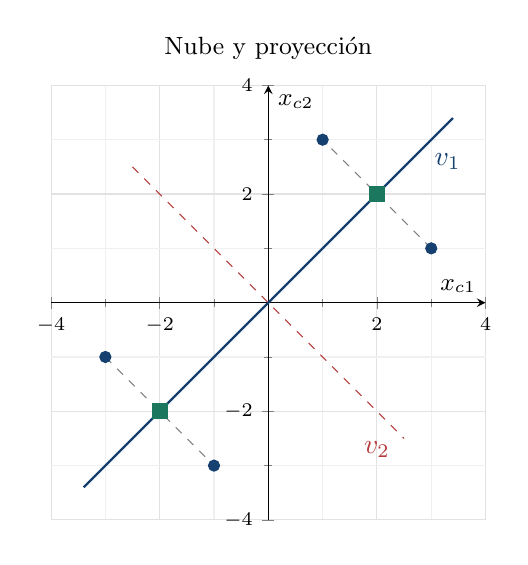
\begin{tikzpicture}
\begin{axis}[base,width=7.6cm,height=7.1cm,axis equal image,xmin=-4,xmax=4,ymin=-4,ymax=4,xlabel={$x_{c1}$},ylabel={$x_{c2}$},title={Nube y proyección},title style={font=\small}]
\addplot[azul,thick,domain=-3.4:3.4]{x};
\addplot[rojo,dashed,domain=-2.5:2.5]{-x};
\addplot[only marks,mark=*,mark size=2pt,azul]coordinates{(2,2)(3,1)(1,3)(-2,-2)(-3,-1)(-1,-3)};
\addplot[only marks,mark=square*,mark size=2.7pt,verde]coordinates{(2,2)(-2,-2)};
\draw[gray,dashed](axis cs:3,1)--(axis cs:2,2)--(axis cs:1,3);
\draw[gray,dashed](axis cs:-3,-1)--(axis cs:-2,-2)--(axis cs:-1,-3);
\node[azul]at(axis cs:3.3,2.6){$v_1$};\node[rojo]at(axis cs:2,-2.7){$v_2$};
\end{axis}
\end{tikzpicture}\hfill
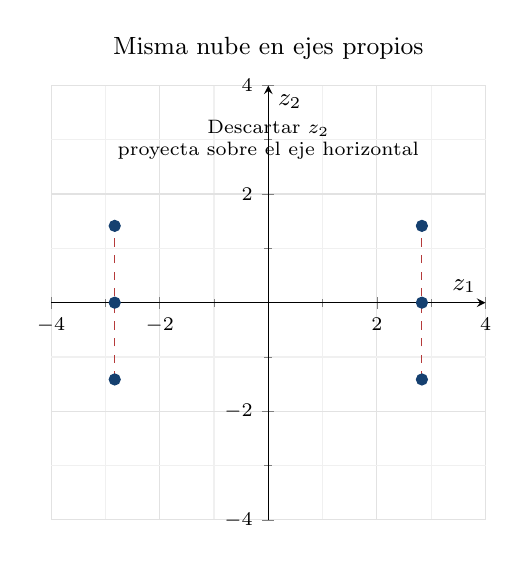
\begin{tikzpicture}
\begin{axis}[base,width=7.6cm,height=7.1cm,axis equal image,xmin=-4,xmax=4,ymin=-4,ymax=4,xlabel={$z_1$},ylabel={$z_2$},title={Misma nube en ejes propios},title style={font=\small}]
\addplot[only marks,mark=*,mark size=2pt,azul]coordinates{(2.828,0)(2.828,1.414)(2.828,-1.414)(-2.828,0)(-2.828,-1.414)(-2.828,1.414)};
\draw[rojo,dashed](axis cs:2.828,-1.414)--(axis cs:2.828,1.414);
\draw[rojo,dashed](axis cs:-2.828,-1.414)--(axis cs:-2.828,1.414);
\node[font=\scriptsize,align=center]at(axis cs:0,3){Descartar $z_2$\\proyecta sobre el eje horizontal};
\end{axis}
\end{tikzpicture}
\caption{Antes de descartar una coordenada, el cambio de base conserva las distancias. Los residuos aparecen verticales en el sistema de componentes.}
\end{figure}

\section{Geometría de elipses: covarianza y precisión}
Si $\Sigma\succ0$ y $\xi\sim N_p(\mu,\Sigma)$, su densidad es proporcional a
\[
\exp\left[-\frac12(x-\mu)\T\Sigma^{-1}(x-\mu)\right],\qquad x,\mu\in\R^{p\times1}.
\]
Con $\Sigma=V\Lambda V\T$ y $z=V\T(x-\mu)\in\R^{p\times1}$, los contornos satisfacen
\[
(x-\mu)\T\Sigma^{-1}(x-\mu)=\sum_{j=1}^p\frac{z_j^2}{\lambda_j}=c.
\]
Los semiejes tienen longitud $\sqrt{c\lambda_j}$. El autovalor mayor corresponde al eje largo de la elipse de covarianza. En cambio, para $x\T\Sigma x=c$, los semiejes son $\sqrt{c/\lambda_j}$: la relación se invierte.
\begin{ejemplo}[Una elipse rotada completamente calculada]
Para $\Sigma=\begin{psmallmatrix}3&1\\1&3\end{psmallmatrix}$, los autovalores son $4$ y $2$ y
\[
\Sigma^{-1}=\frac18\begin{pmatrix}3&-1\\-1&3\end{pmatrix},\qquad
\frac{3x_1^2-2x_1x_2+3x_2^2}{8}=1.
\]
Al definir $z_1=(x_1+x_2)/\sqrt2$ y $z_2=(x_1-x_2)/\sqrt2$, queda $z_1^2/4+z_2^2/2=1$. La elipse tiene semiejes $2$ y $\sqrt2$, rotados $45^\circ$ respecto a las variables originales.
\end{ejemplo}
\begin{figure}[H]\centering
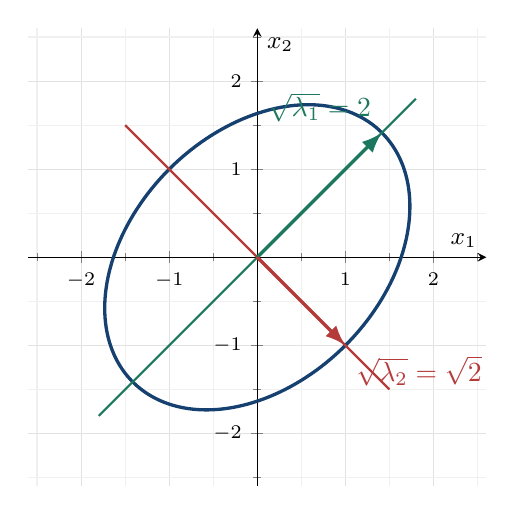
\begin{tikzpicture}
\begin{axis}[base,width=10.5cm,height=7.4cm,axis equal image,xmin=-2.6,xmax=2.6,ymin=-2.6,ymax=2.6,xlabel={$x_1$},ylabel={$x_2$}]
\addplot[azul,very thick,domain=0:360,samples=180]({sqrt(2)*cos(x)+sin(x)},{sqrt(2)*cos(x)-sin(x)});
\addplot[verde,thick,domain=-1.8:1.8]{x};\addplot[rojo,thick,domain=-1.5:1.5]{-x};
\draw[vecverde](axis cs:0,0)--(axis cs:1.4142,1.4142)node[above left]{$\sqrt{\lambda_1}=2$};
\draw[vecrojo](axis cs:0,0)--(axis cs:1,-1)node[below right]{$\sqrt{\lambda_2}=\sqrt2$};
\end{axis}\end{tikzpicture}
\caption{Contorno $x\T\Sigma^{-1}x=1$. Los autovectores fijan direcciones; las raíces de los autovalores fijan longitudes.}
\end{figure}
\subsection{Una figura no normal puede tener los mismos ejes de PCA}
PCA solo necesita segundos momentos. Muchas distribuciones diferentes comparten $\Sigma$ y, por tanto, los mismos ejes y autovalores. La elipse de covarianza describe dispersión cuadrática, pero no prueba normalidad ni determina por sí sola la forma completa de la nube.

\section{Ejemplo de tres variables: de un volumen a un plano}
Considérese la covarianza
\[
\Sigma=\frac16\begin{pmatrix}31&7&16\\7&31&16\\16&16&22\end{pmatrix}\in\R^{3\times3},\quad
v_1=\frac{(1,1,1)\T}{\sqrt3},\quad
v_2=\frac{(1,-1,0)\T}{\sqrt2},\quad
v_3=\frac{(1,1,-2)\T}{\sqrt6}.
\]
Todos los $v_j$ tienen dimensión $3\times1$; sus productos internos cruzados valen cero. Multiplicamos explícitamente:
\[
\Sigma(1,1,1)\T=\frac16(54,54,54)\T=9(1,1,1)\T,
\]
\[
\Sigma(1,-1,0)\T=\frac16(24,-24,0)\T=4(1,-1,0)\T,
\quad \Sigma(1,1,-2)\T=\frac16(6,6,-12)\T=(1,1,-2)\T.
\]
Por tanto, $\Lambda=\diag(9,4,1)$ y $\tr\Sigma=14$. Retener $k=2$ conserva $13/14\approx92.857\%$; retener solo uno conserva $9/14\approx64.286\%$.
\subsection{Proyección concreta y error exacto}
Para $x=(3,1,2)\T\in\R^{3\times1}$, suponiendo media cero,
\[
z_1=v_1\T x=2\sqrt3,\quad z_2=v_2\T x=\sqrt2,\quad z_3=v_3\T x=0.
\]
Este punto ya pertenece al plano principal. Para $y=(3,1,0)\T\in\R^{3\times1}$,
\[
a_1=\frac4{\sqrt3},\quad a_2=\sqrt2,\quad a_3=\frac4{\sqrt6},\qquad
\widehat y=a_1v_1+a_2v_2=(7/3,1/3,4/3)\T,
\]
\[
e=y-\widehat y=(2/3,2/3,-4/3)\T=a_3v_3,\quad
\norm e_2^2=\frac83,\quad v_1\T e=v_2\T e=0.
\]
El plano es $v_3\T y=0$, es decir, $y_1+y_2-2y_3=0$. Su proyector se obtiene sin resolver un nuevo sistema:
\[
P_2=I_3-v_3v_3\T=\frac16\begin{pmatrix}5&-1&2\\-1&5&2\\2&2&2\end{pmatrix},\qquad P_2y=\widehat y.
\]
\begin{figure}[H]\centering
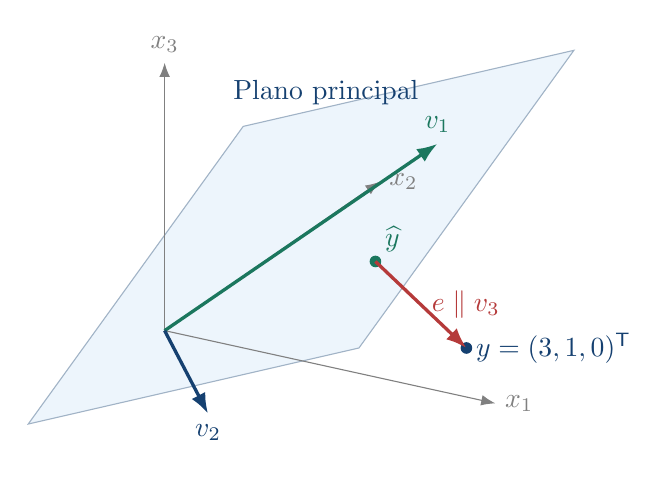
\begin{tikzpicture}[x={(1.0cm,-.22cm)},y={(.65cm,.45cm)},z={(0cm,.9cm)},scale=1.05]
\fill[celeste,opacity=.9](-1,-1,-1)--(3,-1,1)--(3,3,3)--(-1,3,1)--cycle;
\draw[azul!40](-1,-1,-1)--(3,-1,1)--(3,3,3)--(-1,3,1)--cycle;
\draw[eje](0,0,0)--(4,0,0)node[right]{$x_1$};\draw[eje](0,0,0)--(0,4,0)node[right]{$x_2$};\draw[eje](0,0,0)--(0,0,3.6)node[above]{$x_3$};
\draw[vecverde](0,0,0)--(2,2,2)node[above]{$v_1$};
\draw[vec](0,0,0)--(1.5,-1.5,0)node[below]{$v_2$};
\fill[azul](3,1,0)circle(2pt)node[right]{$y=(3,1,0)\T$};
\fill[verde](2.333,.333,1.333)circle(2pt)node[above right]{$\widehat y$};
\draw[vecrojo](2.333,.333,1.333)--(3,1,0)node[midway,right]{$e\parallel v_3$};
\node[azul]at(0,3,1.7){Plano principal};
\end{tikzpicture}
\caption{Reducción de tres variables a dos puntuaciones: el residuo queda en la dirección propia descartada. La perspectiva del dibujo no conserva ángulos.}
\end{figure}

\parte{VII. Escalas, interpretación y descomposición en valores singulares}
\section{Covarianza o correlación: la métrica cambia la respuesta}
Sea $D=\diag(s_1,\ldots,s_p)\in\R^{p\times p}$, donde $s_j=\sqrt{s_{jj}}>0$. Los datos estandarizados son
\[
X_s=X_cD^{-1}\in\R^{n\times p},\quad (X_s)_{ij}=\frac{x_{ij}-\bar x_j}{s_j},\qquad
R=\frac1{n-1}X_s\T X_s=D^{-1}SD^{-1}.
\]
$R$ es la matriz de correlaciones, $r_{jj}=1$ y $\tr R=p$. Aplicar PCA a $R$ da la misma importancia inicial a una desviación estándar en cada variable. Aplicarlo a $S$ da importancia a diferencias medidas en unidades originales.
\begin{ejemplo}[El cambio de unidades puede cambiar el eje dominante]
Si $S=\diag(100,1)$, PCA de covarianzas conserva primero $(1,0)\T$, explicando $100/101$. Pero la correlación es $R=I_2$: ambas direcciones explican lo mismo. Si la primera variable se mide en metros o centímetros, su varianza se multiplica por $10^4$ al cambiar de metros a centímetros. La información observacional no cambió; la distancia euclidiana sí.
\end{ejemplo}
\subsection{Direcciones en coordenadas estandarizadas y originales}
Sea $a\in\R^{p\times1}$ un autovector unitario de $R$ con $Ra=\lambda a$. Su puntuación es
\[
z=X_sa=X_cD^{-1}a=X_cb,\qquad b=D^{-1}a\in\R^{p\times1}.
\]
En general $b\T b\ne1$, pero $b\T D^2b=1$. Además,
\[
D^{-1}SD^{-1}a=\lambda a\quad\Longleftrightarrow\quad Sb=\lambda D^2b.
\]
Se trata de un problema de autovalores generalizados. La reconstrucción original, para $A_k\in\R^{p\times k}$ con columnas propias de $R$, es
\[
\widehat X=\ones_n\bar x\T+X_sA_kA_k\T D.
\]
Minimiza el error estandarizado $\norm{(X-\widehat X)D^{-1}}\F^2$, no necesariamente el error sin ponderar $\norm{X-\widehat X}\F^2$.
\begin{cuidado}[Columnas constantes y criterios de escala]
Si $s_j=0$, no se puede dividir por $s_j$; esa columna no aporta varianza y se retira o se trata explícitamente. Estandarizar no es siempre obligatorio: si todas las variables comparten unidad y sus varianzas diferentes son significativas, PCA de covarianzas puede ser el objetivo adecuado. La elección debe corresponder al error que interesa minimizar.
\end{cuidado}

\section{Interpretar ejes, cargas, puntuaciones y biplots}
Un eje $v_j=(v_{1j},\ldots,v_{pj})\T\in\R^{p\times1}$ define
\[
z_{ij}=v_{1j}(x_{i1}-\bar x_1)+\cdots+v_{pj}(x_{ip}-\bar x_p).
\]
Coeficientes del mismo signo recogen movimientos conjuntos; signos contrarios describen contrastes. Pero el signo global es arbitrario: sustituir $v_j$ por $-v_j$ cambia $z_j$ por $-z_j$ y deja $z_jv_j\T$ igual.
\subsection{Dos usos del término ``carga''}
Algunos textos llaman cargas a los coeficientes $v_{aj}$; otros a correlaciones o a $v_{aj}\sqrt{\lambda_j}$. Hay que especificar la definición. Para la variable $a$, con desviación $s_a>0$, y la puntuación $z_j=X_cv_j\in\R^{n\times1}$,
\[
\widehat{\Cov}(X_a,z_j)=e_a\T Sv_j=\lambda_jv_{aj},\qquad
\boxed{\widehat{\Corr}(X_a,z_j)=\frac{\sqrt{\lambda_j}\,v_{aj}}{s_a}}
\quad(\lambda_j>0),
\]
donde $e_a\in\R^{p\times1}$ es el vector canónico con uno en la posición $a$. Para datos estandarizados $s_a=1$, y la correlación vale $\sqrt{\lambda_j}v_{aj}$.
\subsection{Varianza de cada variable reconstruida}
La covarianza reconstruida es $S_k=V_k\Lambda_kV_k\T$, por lo que
\[
(S_k)_{aa}=\sum_{j=1}^k\lambda_jv_{aj}^2,\qquad
h_a^2=\frac{\sum_{j=1}^k\lambda_jv_{aj}^2}{s_a^2}
=\sum_{j=1}^k\widehat{\Corr}(X_a,z_j)^2\in[0,1].
\]
$h_a^2$ mide qué proporción de la varianza de la variable $a$ conserva la representación. Una proporción global alta puede ocultar una variable mal representada.
\begin{ejemplo}[Cargas en el ejemplo maestro]
Allí $s_1=s_2=\sqrt{28/5}$ y $v_{11}=v_{21}=1/\sqrt2$. Por tanto,
\[
\Corr(X_1,z_1)=\Corr(X_2,z_1)=\sqrt{\frac{48/5}{2(28/5)}}=\sqrt{\frac67}\approx0.92582.
\]
Para la segunda componente las correlaciones son $\sqrt{1/7}$ y $-\sqrt{1/7}$. En cada variable las correlaciones cuadradas suman $6/7+1/7=1$ si conservamos ambos ejes.
\end{ejemplo}
\subsection{Por qué las flechas de un biplot no tienen una escala universal}
Si $X_c\approx U_kD_kV_k\T$, para $0\le\alpha\le1$ podemos escribir
\[
G=U_kD_k^\alpha\in\R^{n\times k},\quad B=V_kD_k^{1-\alpha}\in\R^{p\times k},\qquad
GB\T=U_kD_kV_k\T.
\]
Las filas de $G$ representan observaciones; las filas de $B$, variables. Su producto interno aproxima cada dato centrado. Distintas $\alpha$ cambian longitudes y la interpretación geométrica; solo en escalas adecuadas y con buena representación los ángulos entre flechas aproximan correlaciones.

\section{SVD: existencia, construcción y significado geométrico}
\begin{teorema}[Descomposición en valores singulares compacta]
Toda matriz $X_c\in\R^{n\times p}$ de rango $r$ admite
\[
\boxed{X_c=U_rD_rV_r\T=\sum_{j=1}^rd_j u_jv_j\T},\qquad
U_r\in\R^{n\times r},\ D_r\in\R^{r\times r},\ V_r\in\R^{p\times r},
\]
con $U_r\T U_r=V_r\T V_r=I_r$, $D_r=\diag(d_1,\ldots,d_r)$ y $d_1\ge\cdots\ge d_r>0$. Cada $u_j\in\R^{n\times1}$ y $v_j\in\R^{p\times1}$.
\end{teorema}
\begin{deduccion}
$X_c\T X_c$ es simétrica semidefinida positiva. El teorema espectral da autovectores $v_j$ y autovalores positivos $d_j^2$, $j\le r$. Define $u_j=X_cv_j/d_j$. Entonces
\[
u_i\T u_j=\frac{v_i\T X_c\T X_cv_j}{d_id_j}
=\frac{d_j^2v_i\T v_j}{d_id_j}=\delta_{ij}.
\]
Para $j>r$, $v_j\T X_c\T X_cv_j=\norm{X_cv_j}_2^2=0$, luego $X_cv_j=0$. Al expandir cualquier $x\in\R^{p\times1}$ en la base $\{v_j\}$,
\[
X_cx=\sum_{j=1}^r(v_j\T x)X_cv_j
=\sum_{j=1}^rd_j u_jv_j\T x.
\]
La igualdad para todo $x$ prueba la descomposición matricial.
\end{deduccion}
\subsection{Dos sistemas de coordenadas diferentes}
\[
X_cv_j=d_ju_j,\qquad X_c\T u_j=d_jv_j,\qquad
X_c\T X_cv_j=d_j^2v_j,\qquad X_cX_c\T u_j=d_j^2u_j.
\]
$V_r$ vive en el espacio de variables, dimensión $p$; $U_r$ vive en el espacio de observaciones, dimensión $n$. $X_c$ puede ser rectangular y por eso no tiene sentido general pedirle una ecuación $X_cv=\lambda v$: los dos lados tendrían dimensiones distintas.
\subsection{SVD completa y formas reducidas}
La SVD completa utiliza $U\in\R^{n\times n}$, $V\in\R^{p\times p}$ y una matriz diagonal rectangular $D\in\R^{n\times p}$. La SVD económica suele conservar $\min(n,p)$ columnas, algunas asociadas a ceros; la compacta conserva solo las $r$ positivas. No son convenciones idénticas.
\subsection{El puente exacto con PCA}
\[
S=\frac1{n-1}V_rD_r^2V_r\T,\qquad
\boxed{\lambda_j=\frac{d_j^2}{n-1}},\quad
\boxed{Z_r=X_cV_r=U_rD_r},\quad
\boxed{\widehat X_c=U_kD_kV_k\T}.
\]
Los valores singulares no son las varianzas; sus cuadrados, divididos por $n-1$, sí. Los vectores de $U_r$ no son puntuaciones con su escala original; hay que multiplicarlos por $D_r$.
\begin{idea}[Una descomposición, dos interpretaciones]
En álgebra, $X_c$ transforma direcciones $v_j$ en direcciones $u_j$, escaladas por $d_j$. En estadística, $v_j$ define una combinación de variables y $d_ju_j$ contiene sus puntuaciones en las $n$ observaciones.
\end{idea}

\section{SVD exacta del ejemplo maestro y la versión dual}
En la sección \ref{sec:ejemplo2d}, $n=6$, $p=r=2$:
\[
D_2=\begin{pmatrix}4\sqrt3&0\\0&2\sqrt2\end{pmatrix},\quad
u_1=\frac1{\sqrt6}(1,1,1,-1,-1,-1)\T\in\R^{6\times1},
\]
\[
u_2=\frac12(0,1,-1,0,-1,1)\T\in\R^{6\times1},\quad
U_2=[u_1\ u_2]\in\R^{6\times2},\quad
V_2=\frac1{\sqrt2}\begin{pmatrix}1&1\\1&-1\end{pmatrix}.
\]
Comprobamos $u_1\T u_1=6/6=1$, $u_2\T u_2=4/4=1$ y $u_1\T u_2=0$. Luego
\[
X_c=4\sqrt3\,u_1v_1\T+2\sqrt2\,u_2v_2\T,\quad
Z_1=4\sqrt3\,u_1,\quad \widehat X_c=4\sqrt3\,u_1v_1\T.
\]
La segunda pieza es exactamente la matriz residual calculada antes. Los valores singulares positivos son $d_1\approx6.928203$ y $d_2\approx2.828427$; sus cuadrados son $48$ y $8$.
\subsection{Cuando hay muchas más variables que observaciones}
Si $p\gg n$, formar una covarianza $p\times p$ puede ser caro. Podemos diagonalizar
\[
G=\frac1{n-1}X_cX_c\T\in\R^{n\times n},\qquad Gu_j=\lambda_ju_j.
\]
Para $\lambda_j>0$,
\[
v_j=\frac{X_c\T u_j}{\sqrt{(n-1)\lambda_j}}\in\R^{p\times1},\qquad
\norm{v_j}_2^2=\frac{u_j\T X_cX_c\T u_j}{(n-1)\lambda_j}=1,
\]
\[
Sv_j=\frac{X_c\T X_cX_c\T u_j}{(n-1)\sqrt{(n-1)\lambda_j}}=\lambda_jv_j.
\]
Esto recupera las mismas direcciones. No se divide por $\lambda_j=0$. En cómputo numérico, una SVD directa o truncada suele ser preferible a construir productos de Gram cuando preocupan precisión y condicionamiento.

\section{Eckart--Young--Mirsky: la mejor aproximación de rango bajo}
\begin{teorema}[Optimalidad en Frobenius y norma espectral]
Sea $X_c=\sum_{j=1}^rd_ju_jv_j\T$ y $1\le k<r$. Entre todas las matrices $B\in\R^{n\times p}$ con $\rank B\le k$, la truncación $X_{c,k}=\sum_{j=1}^kd_ju_jv_j\T$ satisface
\[
\min_{\rank B\le k}\norm{X_c-B}\F^2=\sum_{j=k+1}^rd_j^2,\qquad
\min_{\rank B\le k}\norm{X_c-B}_2=d_{k+1},
\]
donde $\norm A_2=\max_{\norm x_2=1}\norm{Ax}_2$ es la norma matricial espectral.
\end{teorema}
\begin{deduccion}
\textbf{Frobenius.} Sea $P$ el proyector ortogonal sobre el espacio de filas de $B$, de rango $q\le k$. Entonces $B=BP$ y
\[
X_c-B=X_c(I_p-P)+(X_cP-B).
\]
Ambos sumandos son ortogonales para el producto de Frobenius porque sus filas pertenecen a subespacios ortogonales. Por tanto,
\[
\norm{X_c-B}\F^2=\norm{X_c(I_p-P)}\F^2+\norm{X_cP-B}\F^2
\ge\norm{X_c}\F^2-\tr(PX_c\T X_c).
\]
El principio de máxima traza implica $\tr(PX_c\T X_c)\le\sum_{j=1}^q d_j^2\le\sum_{j=1}^kd_j^2$. Esto da la cota inferior. La truncación la alcanza porque sus términos residuales $d_ju_jv_j\T$ son ortogonales y tienen norma de Frobenius $d_j$.

\textbf{Espectral.} El subespacio $M=\spanop\{v_1,\ldots,v_{k+1}\}$ tiene dimensión $k+1$, mientras que $B$ tiene rango a lo sumo $k$. Existe $a\in M\cap\kerop B$, $\norm a_2=1$. Entonces
\[
\norm{X_c-B}_2\ge\norm{(X_c-B)a}_2=\norm{X_ca}_2
=\left(\sum_{j=1}^{k+1}d_j^2(v_j\T a)^2\right)^{1/2}\ge d_{k+1}.
\]
Para la truncación, el mayor valor singular del residuo es precisamente $d_{k+1}$, así que alcanza la cota.
\end{deduccion}
\subsection{Unicidad y degeneración}
Si $d_k>d_{k+1}$, la aproximación de rango $k$ óptima en Frobenius es única. Si el corte atraviesa un grupo de valores singulares iguales, distintas elecciones dentro de ese subespacio pueden producir diferentes aproximaciones con el mismo error. La unicidad en norma espectral es una cuestión distinta: no se deduce de la misma condición sin más.
\subsection{Compresión de una matriz y de una imagen}
Guardar $X_c$ requiere $np$ números. Una representación factorizada de rango $k$ utiliza aproximadamente $nk+pk+k$, además de la media si corresponde. Por ejemplo, para $n=1000$, $p=500$, $k=10$, son $15010$ números frente a $500000$. La reducción real de almacenamiento depende de precisión, formato y metadatos. Para una imagen matricial, la SVD aproxima intensidades; no exige interpretar filas como observaciones estadísticas.

\section{Varianza explicada, elección de dimensión y distancias}
Para $\tr S>0$, definimos
\[
\rho_j=\frac{\lambda_j}{\sum_{\ell=1}^p\lambda_\ell},\qquad
C_k=\sum_{j=1}^k\rho_j,\qquad
1-C_k=\frac{\norm{X_c-X_{c,k}}\F^2}{\norm{X_c}\F^2}.
\]
Una regla descriptiva es elegir el menor $k$ con $C_k\ge\tau$, por ejemplo $\tau=0.95$. El umbral es una decisión sobre error relativo de reconstrucción; no una ley estadística ni garantía predictiva.
\begin{ejemplo}[Un espectro que permite comparar criterios]
Sean los autovalores $(9,4,1,0.5,0.3,0.2)$, de suma $15$. Entonces
\[
(C_1,C_2,C_3,C_4,C_5,C_6)=(0.6,0.866667,0.933333,0.966667,0.986667,1).
\]
El $90\%$ exige tres componentes; el $95\%$, cuatro. El codo visual podría sugerir dos, pero eso responde a otro criterio y deja $13.333\%$ de varianza fuera.
\end{ejemplo}
\begin{figure}[H]\centering
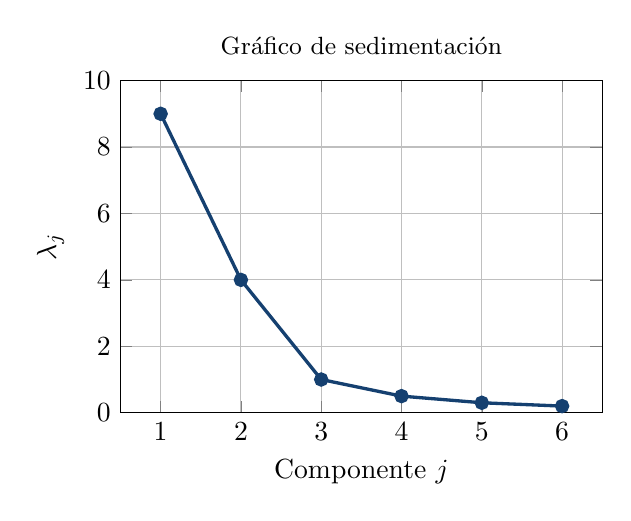
\begin{tikzpicture}
\begin{axis}[width=7.7cm,height=5.8cm,xlabel={Componente $j$},ylabel={$\lambda_j$},xtick={1,2,3,4,5,6},ymin=0,ymax=10,grid=major,title={Gráfico de sedimentación},title style={font=\small}]
\addplot[azul,very thick,mark=*]coordinates{(1,9)(2,4)(3,1)(4,.5)(5,.3)(6,.2)};
\end{axis}\end{tikzpicture}\hfill
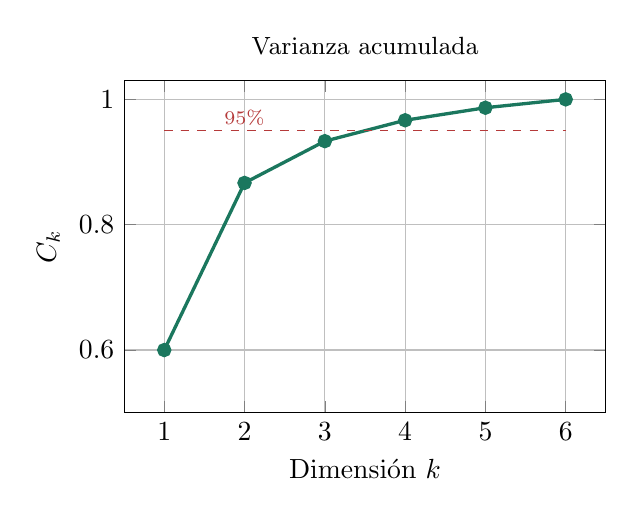
\begin{tikzpicture}
\begin{axis}[width=7.7cm,height=5.8cm,xlabel={Dimensión $k$},ylabel={$C_k$},xtick={1,2,3,4,5,6},ymin=.5,ymax=1.03,grid=major,title={Varianza acumulada},title style={font=\small}]
\addplot[verde,very thick,mark=*]coordinates{(1,.6)(2,.866667)(3,.933333)(4,.966667)(5,.986667)(6,1)};
\addplot[rojo,dashed,domain=1:6]{.95};\node[rojo,font=\scriptsize]at(axis cs:2,.97){$95\%$};
\end{axis}\end{tikzpicture}
\caption{Codo y umbral de varianza son herramientas distintas. La selección para predicción debe evaluar además el resultado supervisado.}
\end{figure}
\subsection{Criterios adicionales y sus límites}
El análisis paralelo compara autovalores observados con los de datos de referencia simulados bajo un modelo sin estructura común; depende de cómo se defina esa referencia. La validación de reconstrucción debe evaluar observaciones o entradas no usadas para ajustar; si solo se proyectan observaciones nuevas completas y se permite aumentar $k$ sin coste, el error disminuye al conservar más dimensiones. Para seleccionar un $k$ parsimonioso se necesita penalización, un objetivo de ruido o validación de entradas ocultas. En tareas supervisadas se elige $k$ dentro de la validación del predictor.
\subsection{PCA no conserva cada distancia con el mismo porcentaje}
Para dos observaciones $x_i,x_\ell\in\R^{p\times1}$, define $d=x_i-x_\ell$. Entonces
\[
\norm d_2^2=\norm{V_k\T d}_2^2+\norm{(I_p-P_k)d}_2^2,
\quad 0\le\norm{V_k\T d}_2^2\le\norm d_2^2.
\]
Cada distancia solo disminuye, pero puede colapsar totalmente si $d$ está en el espacio descartado. Sí hay una identidad global:
\[
\sum_{i<\ell}\norm{x_i-x_\ell}_2^2=n\sum_i\norm{x_i-\bar x}_2^2=n\norm{X_c}\F^2.
\]
\textbf{Demostración.} La suma sobre todos los pares ordenados es $2n\sum_i\norm{x_i}_2^2-2\norm{\sum_ix_i}_2^2$; dividir por dos y centrar da el resultado. Aplicando la identidad a los residuos, PCA minimiza la \emph{suma} de pérdidas de distancias cuadradas entre pares para proyecciones ortogonales de dimensión $k$; no la peor distorsión relativa.

\section{Blanqueamiento, Mahalanobis y la geometría de identidad}
Supón $S\succ0$ y $S=V\Lambda V\T$. Los datos de PCA rotados $Z=X_cV$ tienen covarianza $\Lambda$, que es diagonal pero no suele ser identidad. Para hacerla identidad se escala:
\[
W_{\mathrm{PCA}}=X_cV\Lambda^{-1/2}\in\R^{n\times p},\qquad
\frac1{n-1}W_{\mathrm{PCA}}\T W_{\mathrm{PCA}}=I_p.
\]
Este es el blanqueamiento PCA. El blanqueamiento simétrico o ZCA es
\[
W_{\mathrm{ZCA}}=X_cS^{-1/2}=X_cV\Lambda^{-1/2}V\T\in\R^{n\times p}.
\]
También tiene covarianza identidad, pero vuelve a las coordenadas originales mediante $V\T$.
\subsection{Mahalanobis se vuelve Euclides}
Para $x,y\in\R^{p\times1}$,
\[
d_M(x,y)^2=(x-y)\T S^{-1}(x-y)
=\norm{\Lambda^{-1/2}V\T(x-y)}_2^2.
\]
Una diferencia grande en una dirección muy variable cuenta menos; una diferencia pequeña en una dirección de varianza minúscula puede contar mucho. Esto explica por qué blanquear puede amplificar ruido si hay autovalores muy pequeños.
\begin{ejemplo}[La identidad aparece por una transformación, no por casualidad]
Para $S=\begin{psmallmatrix}3&1\\1&3\end{psmallmatrix}$, $\Lambda=\diag(4,2)$. Si $z=(z_1,z_2)\T$ son coordenadas principales,
\[
w=(z_1/2,z_2/\sqrt2)\T\in\R^{2\times1},\qquad\Cov(w)=I_2.
\]
PCA solo dio covarianza $\diag(4,2)$; dividir por las desviaciones $2$ y $\sqrt2$ es el paso adicional.
\end{ejemplo}
\subsection{Singularidad, pseudoinversa y regularización}
Si solo hay $r<p$ autovalores positivos, $S^{-1}$ no existe. La pseudoinversa es
\[
S^+=V_r\Lambda_r^{-1}V_r\T\in\R^{p\times p}.
\]
Se puede blanquear a $r$ dimensiones mediante $X_cV_r\Lambda_r^{-1/2}$, cuya covarianza es $I_r$. En $p$ dimensiones, $S^{+1/2}SS^{+1/2}=V_rV_r\T$, un proyector, no $I_p$. Usar $(S+\alpha I_p)^{-1/2}$ con $\alpha>0$ evita divisiones extremas, pero la covarianza transformada tiene autovalores $\lambda_j/(\lambda_j+\alpha)$, no exactamente uno.

\parte{VIII. Estimación, MCO y GLS: momentos de coeficientes y predicciones}
\section{Parámetros, estimadores, sesgo, riesgo y convergencia}
Un parámetro $\theta\in\R^d$ es una cantidad fija del modelo. Un estimador $\widehat\theta=T(D)$ es una función de los datos aleatorios $D$, por tanto una variable o vector aleatorio. Su valor calculado en una muestra es una \emph{estimación}. Si existen los momentos,
\[
b(\theta)=\E\widehat\theta-\theta,\quad
V(\theta)=\Cov(\widehat\theta),\quad
\E[(\widehat\theta-\theta)(\widehat\theta-\theta)\T]=V+bb\T.
\]
Tomar traza da el riesgo cuadrático $\E\norm{\widehat\theta-\theta}_2^2=\tr V+\norm b_2^2$. Un estimador sesgado puede tener menor riesgo que uno insesgado si reduce suficiente varianza.
\subsection{La media converge por una desigualdad elemental}
Para una variable no negativa $W$, $\E W\ge t\Prob(W\ge t)$, de donde $\Prob(W\ge t)\le\E W/t$ (Markov). Aplicándola a $(U-\E U)^2$ obtenemos Chebyshev. Si $U_i$ son independientes e idénticamente distribuidas con varianza $\sigma^2$,
\[
\Prob(|\bar U-\mu|\ge\varepsilon)\le\frac{\sigma^2}{n\varepsilon^2}\to0.
\]
Esto prueba consistencia de la media con varianza finita. Para $x_i\in\R^p$, $p$ fijo,
\[
\Prob(\norm{\bar x-\mu}_2\ge\varepsilon)
\le\frac{\tr\Sigma}{n\varepsilon^2}.
\]
Si $p$ crece con $n$, esta misma cota necesita que $\tr\Sigma/n\to0$ para garantizar convergencia en norma; la consistencia de cada coordenada no asegura consistencia del vector entero.
\subsection{Límite normal multivariado y método delta}
Para $x_i$ i.i.d. con segundos momentos finitos y dimensión fija,
\[
\sqrt n(\bar x-\mu)\xrightarrow{d}\mathcal N_p(0,\Sigma).
\]
Una justificación usa cualquier vector $a$: la función característica de $a\T(x_i-\mu)$, cerca de cero, es $1-t^2a\T\Sigma a/2+o(t^2)$. La de su suma dividida por $\sqrt n$ es la potencia $n$ de esa expresión evaluada en $t/\sqrt n$, que tiende a $e^{-t^2a\T\Sigma a/2}$. El criterio de Cramér--Wold reúne todas esas proyecciones escalares en el límite vectorial. Este argumento usa el teorema de continuidad de funciones características.
Si $\sqrt n(\widehat\theta-\theta)\xrightarrow d\mathcal N_d(0,V)$ y $g$ es diferenciable en $\theta$,
\[
\sqrt n(g(\widehat\theta)-g(\theta))\xrightarrow d
\mathcal N_m(0,J_g(\theta)VJ_g(\theta)\T).
\]
Se deduce por Taylor y porque el resto es menor que $\norm{\widehat\theta-\theta}$. La covarianza del límite es $JVJ\T$; la covarianza aproximada del estimador es $JVJ\T/n$. Convergencia en distribución no garantiza convergencia de esperanzas o varianzas sin condiciones de integrabilidad uniforme.

\section{MCO: deducción desde sumas hasta el estimador matricial}
El modelo lineal es
\[
y=X\beta+u,\quad y,u\in\R^{n\times1},\quad X\in\R^{n\times p},\quad\beta\in\R^{p\times1}.
\]
Aquí $p$ cuenta \emph{todos} los coeficientes, incluido el intercepto si hay una columna de unos. Las filas de $X$ son $x_i\T$. Por ahora $X$ tiene rango columna $p$, así que $n\ge p$. MCO minimiza
\[
L(b)=\sum_{i=1}^n\left(y_i-\sum_{j=1}^px_{ij}b_j\right)^2
=(y-Xb)\T(y-Xb).
\]
Expandir da $y\T y-2b\T X\T y+b\T X\T Xb$. Por coordenadas,
\[
\frac{\partial L}{\partial b_k}=-2\sum_i x_{ik}y_i
+2\sum_i\sum_jx_{ik}x_{ij}b_j.
\]
Las $p$ condiciones se reúnen en $X\T Xb=X\T y$, y
\[
\boxed{\widehat\beta=(X\T X)^{-1}X\T y},\qquad
H_X=X(X\T X)^{-1}X\T,\qquad M_X=I_n-H_X.
\]
Como $a\T X\T Xa=\norm{Xa}_2^2>0$ para $a\ne0$, la Hessiana $2X\T X$ es positiva definida y el mínimo único. $\widehat y=H_Xy$ es la proyección de la respuesta sobre el espacio de columnas de $X$; $\widehat u=M_Xy$ es el residuo, con $X\T\widehat u=0$.
\subsection{Esperanza y sesgo condicional, sin ocultar exogeneidad}
Sea $A_X=(X\T X)^{-1}X\T$. Sustituyendo el modelo,
\[
\widehat\beta=\beta+A_Xu,
\quad\E(\widehat\beta\mid X)=\beta+A_X\E(u\mid X).
\]
La hipótesis $\E(u\mid X)=0$ da insesgamiento condicional exacto. La covarianza, con $\Omega_X=\Cov(u\mid X)$, es
\[
\boxed{\Cov(\widehat\beta\mid X)=
(X\T X)^{-1}X\T\Omega_X X(X\T X)^{-1}}.
\]
No hemos supuesto normalidad, homocedasticidad ni errores independientes. Si $\Omega_X=\sigma^2I_n$, se reduce a $\sigma^2(X\T X)^{-1}$. Esa reducción no se permite si hay varianzas distintas o correlación entre observaciones.
\subsection{Cada coeficiente es una combinación de todos los errores}
Si $a_j\T$ es la fila $j$ de $A_X$,
\[
\widehat\beta_j-\beta_j=\sum_i a_{ji}u_i,
\quad\Cov(\widehat\beta_j,\widehat\beta_k\mid X)
=\sum_{i,\ell}a_{ji}a_{k\ell}(\Omega_X)_{i\ell}.
\]
En homocedasticidad, $\Var(\widehat\beta_j\mid X)=\sigma^2[(X\T X)^{-1}]_{jj}$. La covarianza entre coeficientes depende de entradas \emph{fuera} de la diagonal de la inversa, no de las correlaciones de las columnas tomadas aisladamente.
\subsection{Esperanza y covarianza no condicionadas}
Si $X$ es aleatoria y se cumple exogeneidad condicional, con momentos suficientes,
\[
\E\widehat\beta=\beta,\qquad
\Cov(\widehat\beta)=\E[\Cov(\widehat\beta\mid X)].
\]
Si la media condicional no es $\beta$, se añade $\Cov(\E(\widehat\beta\mid X))$ por la ley de covarianza total. La expresión $\sigma^2[\E(X\T X)]^{-1}$ generalmente no es la covarianza: esperanza e inversión no conmutan.

\section{Predicciones, residuos y varianza residual: todos sus momentos}
Supongamos $\E(u\mid X)=0$ y $\Cov(u\mid X)=\sigma^2I_n$. Condicionalmente a $X$,
\[
\E\widehat y=X\beta,\quad\Cov(\widehat y)=\sigma^2H_X,
\qquad\E\widehat u=0,\quad\Cov(\widehat u)=\sigma^2M_X.
\]
Las matrices son proyecciones simétricas de rangos $p$ y $n-p$. Como $H_XM_X=0$,
\[
\Cov(\widehat y,\widehat u\mid X)=0,\quad
\Cov(\widehat\beta,\widehat u\mid X)=0.
\]
Estos resultados son incorrelación; con errores gaussianos pasan a independencia. Si $h_{ii}$ es la diagonal de $H_X$, $\Var(\widehat u_i\mid X)=\sigma^2(1-h_{ii})$ y $\Cov(\widehat u_i,\widehat u_j\mid X)=-\sigma^2h_{ij}$ para $i\ne j$. Aunque los errores originales sean independientes, los residuos normalmente no lo son.
\subsection{Deducir el divisor de la estimación de ruido}
Como $\widehat u=M_Xu$,
\[
\E(\widehat u\T\widehat u\mid X)=\E(u\T M_Xu\mid X)
=\sigma^2\tr M_X=\sigma^2(n-p).
\]
Para $n>p$, $s^2=\widehat u\T\widehat u/(n-p)$ es insesgado para $\sigma^2$. Si $n=p$ y $X$ es invertible, ajustamos exactamente cualquier $y$ y no quedan grados de libertad para estimar ruido mediante residuos.
\subsection{Predicción nueva: media frente a observación}
Para una fila nueva determinista $x_0\T$, $\widehat m_0=x_0\T\widehat\beta$ estima $m_0=x_0\T\beta$ y
\[
\E(\widehat m_0\mid X)=m_0,\quad
\Var(\widehat m_0\mid X)=\sigma^2x_0\T(X\T X)^{-1}x_0.
\]
Si $y_0=m_0+u_0$ y $u_0$ es independiente de la muestra, con varianza $\sigma^2$, el error $y_0-\widehat m_0$ tiene varianza $\sigma^2[1+x_0\T(X\T X)^{-1}x_0]$. El término uno representa ruido irreducible de la observación nueva. Para un bloque $X_0\in\R^{m\times p}$ de puntos nuevos, la covarianza de sus medias estimadas es $\sigma^2X_0(X\T X)^{-1}X_0\T$; las predicciones comparten incertidumbre de coeficientes.

\section{MCO normal: distribución exacta, Student y pruebas conjuntas}
Añadimos $u\mid X\sim\mathcal N_n(0,\sigma^2I_n)$. Como MCO es una transformación lineal,
\[
\widehat\beta\mid X\sim\mathcal N_p\!\left(\beta,\sigma^2(X\T X)^{-1}\right).
\]
Una rotación ortogonal diagonaliza $M_X$ en $n-p$ unos y $p$ ceros. La forma cuadrática de una normal estándar produce
\[
\frac{(n-p)s^2}{\sigma^2}=\frac{u\T M_Xu}{\sigma^2}\sim\chi^2_{n-p},
\quad\Var(s^2\mid X)=\frac{2\sigma^4}{n-p}.
\]
El vector $\widehat\beta$ es independiente de $\widehat u$ por normalidad conjunta y covarianza cruzada cero, y por tanto de $s^2$. Así,
\[
\boxed{\frac{\widehat\beta_j-\beta_j}{s\sqrt{[(X\T X)^{-1}]_{jj}}}\mid X\sim t_{n-p}}.
\]
Para una combinación $c\T\beta$, reemplazamos la entrada diagonal por $c\T(X\T X)^{-1}c$. Un intervalo con cobertura $1-\alpha$ utiliza el cuantil $t_{n-p,1-\alpha/2}$; los resultados son exactos bajo las hipótesis, no por la mera presencia de una regresión lineal.
\subsection{Varias restricciones y una forma cuadrática}
Para $R\in\R^{q\times p}$ de rango fila $q$ y la hipótesis $R\beta=r$, define $C=R(X\T X)^{-1}R\T$. Bajo la hipótesis,
\[
(R\widehat\beta-r)\T C^{-1}(R\widehat\beta-r)/\sigma^2\sim\chi^2_q.
\]
Es independiente de $(n-p)s^2/\sigma^2$. Por la definición de Fisher,
\[
F=\frac{(R\widehat\beta-r)\T C^{-1}(R\widehat\beta-r)}{q s^2}\sim F_{q,n-p}.
\]
No se obtienen $q$ pruebas independientes simplemente porque haya $q$ coeficientes: la covarianza conjunta es parte de la forma cuadrática.
\subsection{Distribución de la covarianza estimada}
Con $G=(X\T X)^{-1}$, $\widehat V=s^2G$ estima $\Cov(\widehat\beta\mid X)$. Entonces
\[
\E(\widehat V_{ij}\mid X)=\sigma^2G_{ij},\quad
\Cov(\widehat V_{ij},\widehat V_{k\ell}\mid X)
=\frac{2\sigma^4}{n-p}G_{ij}G_{k\ell}.
\]
Todas sus entradas fluctúan mediante el mismo escalar $s^2$ cuando $X$ está fija. La matriz estimada no tiene una Wishart ordinaria independiente entrada por entrada.

\section{Ejemplo completo de MCO con intercepto y pendiente}
Consideremos
\[
X=\begin{pmatrix}1&-2\\1&-1\\1&0\\1&1\\1&2\end{pmatrix},\quad
y=\begin{pmatrix}-2\\-3\\3\\1\\6\end{pmatrix},\quad
X\T X=\begin{pmatrix}5&0\\0&10\end{pmatrix},\quad X\T y=\begin{pmatrix}5\\20\end{pmatrix}.
\]
Por tanto $\widehat\beta=(1,2)\T$, $\widehat y=(-3,-1,1,3,5)\T$ y $\widehat u=(1,-2,2,-2,1)\T$. Comprobamos $\sum_i\widehat u_i=0$ y $\sum_i x_i\widehat u_i=0$.
\[
\operatorname{SSE}=14,\quad s^2=14/3,\quad
\widehat V=\begin{pmatrix}14/15&0\\0&7/15\end{pmatrix}.
\]
Los errores estándar del intercepto y pendiente son $\sqrt{14/15}$ y $\sqrt{7/15}$. Para un punto con coordenada $3$, $x_0=(1,3)\T$,
\[
\widehat m_0=7,\quad\widehat{\Var}(\widehat m_0)=\frac{14}3\left(\frac15+\frac9{10}\right)=\frac{77}{15},
\quad\widehat{\Var}(y_0-\widehat m_0)=\frac{49}5.
\]
La covarianza intercepto--pendiente es cero porque el predictor está centrado; trasladar el origen del predictor puede cambiar esa covarianza sin cambiar la recta ajustada.
\subsection{La fórmula escalar general sale de invertir una matriz dos por dos}
Con $x_i$ escalar, $\bar x=n^{-1}\sum_i x_i$ y $S_{xx}=\sum_i(x_i-\bar x)^2>0$,
\[
\widehat\beta_1=\frac{\sum_i(x_i-\bar x)(y_i-\bar y)}{S_{xx}},\quad
\widehat\beta_0=\bar y-\widehat\beta_1\bar x.
\]
En homocedasticidad,
\[
\Var(\widehat\beta_1\mid X)=\frac{\sigma^2}{S_{xx}},\quad
\Var(\widehat\beta_0\mid X)=\sigma^2\left(\frac1n+\frac{\bar x^2}{S_{xx}}\right),\quad
\Cov(\widehat\beta_0,\widehat\beta_1\mid X)=-\frac{\sigma^2\bar x}{S_{xx}}.
\]
La pendiente se estima peor cuando los valores de $x$ se parecen mucho. El intercepto se estima peor si el cero está lejos del centro observado.
\begin{figure}[H]\centering
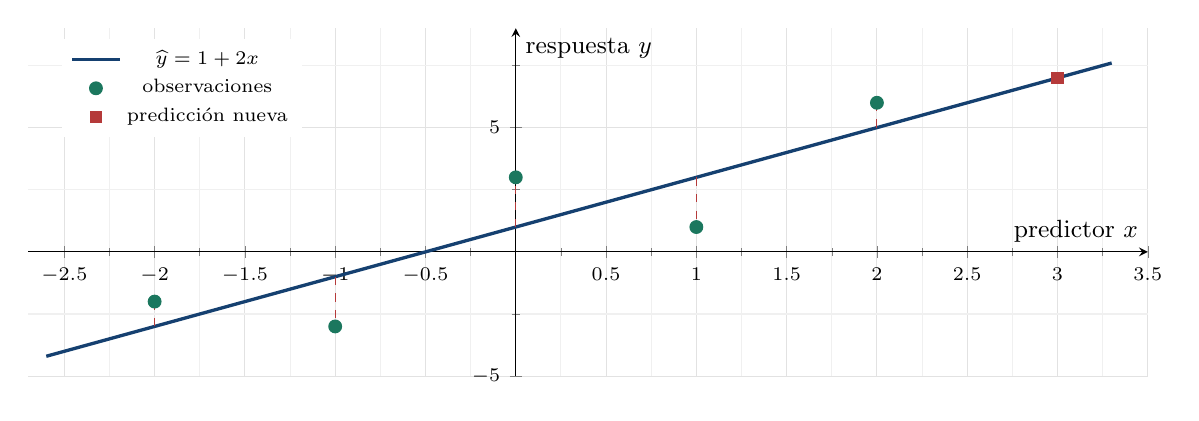
\begin{tikzpicture}\begin{axis}[base,width=15.8cm,height=6cm,xmin=-2.7,xmax=3.5,ymin=-5,ymax=9,xlabel={predictor $x$},ylabel={respuesta $y$},legend pos=north west]
\addplot[azul,very thick,domain=-2.6:3.3]{1+2*x};\addlegendentry{$\widehat y=1+2x$}
\addplot[only marks,mark=*,mark size=2.3pt,verde]coordinates{(-2,-2)(-1,-3)(0,3)(1,1)(2,6)};\addlegendentry{observaciones}
\draw[rojo,dashed](axis cs:-2,-3)--(axis cs:-2,-2);
\draw[rojo,dashed](axis cs:-1,-1)--(axis cs:-1,-3);
\draw[rojo,dashed](axis cs:0,1)--(axis cs:0,3);
\draw[rojo,dashed](axis cs:1,3)--(axis cs:1,1);
\draw[rojo,dashed](axis cs:2,5)--(axis cs:2,6);
\addplot[only marks,mark=square*,rojo]coordinates{(3,7)};\addlegendentry{predicción nueva}
\end{axis}\end{tikzpicture}
\caption{MCO minimiza residuos verticales en el espacio predictor--respuesta. La ortogonalidad de residuos y columnas ocurre en el espacio de $n$ observaciones.}
\end{figure}

\section{Gauss--Markov, controles y sesgo por omisión}
\begin{teorema}[MCO es el mejor estimador lineal insesgado bajo esfericidad]
Con $X$ fija de rango $p$, $\E u=0$ y $\Cov(u)=\sigma^2I_n$, todo estimador $Ly$ con $LX=I_p$ tiene covarianza mayor o igual que MCO en el orden semidefinido.
\end{teorema}
\begin{deduccion}
Escribe $L=A_X+D$. Insesgamiento implica $DX=0$. Entonces $A_XD\T=(X\T X)^{-1}X\T D\T=0$, y
\[
\Cov(Ly)-\Cov(\widehat\beta)=\sigma^2DD\T\succeq0.
\]
Para cualquier combinación $c\T\beta$, la diferencia de varianzas es $\sigma^2\norm{D\T c}_2^2\ge0$. La prueba no utiliza normalidad. ``Mejor'' se refiere a esta clase lineal insesgada, no a todos los estimadores posibles bajo cualquier pérdida.
\end{deduccion}
\subsection{Frisch--Waugh--Lovell por eliminación de bloques}
Particiona $X=[X_1\ X_2]$. Las ecuaciones normales son
\[
X_1\T X_1b_1+X_1\T X_2b_2=X_1\T y,\quad
X_2\T X_1b_1+X_2\T X_2b_2=X_2\T y.
\]
Despejar $b_1$ y sustituir da
\[
\boxed{\widehat\beta_2=(X_2\T M_1X_2)^{-1}X_2\T M_1y},\quad
M_1=I-X_1(X_1\T X_1)^{-1}X_1\T.
\]
Se residualizan respuesta y predictores respecto a $X_1$. Bajo homocedasticidad,
\[
\E(\widehat\beta_2\mid X)=\beta_2,\quad
\Cov(\widehat\beta_2\mid X)=\sigma^2(X_2\T M_1X_2)^{-1}.
\]
Esto explica matemáticamente ``controlar por otras variables'': solo la variación de $X_2$ fuera del espacio de $X_1$ identifica su coeficiente.
\subsection{Omitir un bloque relevante}
Si el modelo verdadero es $y=X_1\beta_1+X_2\beta_2+u$, pero ajustamos solo $X_1$,
\[
\E(\widetilde\beta_1\mid X)=\beta_1+(X_1\T X_1)^{-1}X_1\T X_2\beta_2.
\]
El sesgo desaparece si $\beta_2=0$ o si $X_1\T X_2=0$, pero no por aumentar automáticamente $n$. Un regresor omitido correlacionado con uno incluido genera una parte sistemática del error que viola exogeneidad.

\section{GLS, WLS y covarianzas robustas}
Si $\Omega\succ0$ es conocida y $\E(u\mid X)=0$, la pérdida natural es la distancia de Mahalanobis
\[
L(b)=(y-Xb)\T\Omega^{-1}(y-Xb).
\]
Derivar da
\[
\boxed{\widehat\beta_{\rm GLS}=(X\T\Omega^{-1}X)^{-1}X\T\Omega^{-1}y},\quad
\Cov(\widehat\beta_{\rm GLS}\mid X)=(X\T\Omega^{-1}X)^{-1}.
\]
Se interpreta como MCO sobre $\widetilde y=\Omega^{-1/2}y$, $\widetilde X=\Omega^{-1/2}X$. Si $\Omega=\sigma^2W^{-1}$, aparece $\sigma^2(X\T WX)^{-1}$ como covarianza; si $W$ es diagonal son mínimos cuadrados ponderados.
\subsection{Normalidad y máxima verosimilitud}
Para $u\mid X\sim\mathcal N_n(0,\Omega)$, el logaritmo de la verosimilitud, salvo constantes, es $-\tfrac12\log\det\Omega-\tfrac12(y-X\beta)\T\Omega^{-1}(y-X\beta)$. Su score es $X\T\Omega^{-1}(y-X\beta)$ y la información de Fisher $X\T\Omega^{-1}X$. El estimador GLS tiene exactamente la inversa de esa información como covarianza. Si estimamos $\Omega$, la sustitución produce GLS factible; sus momentos finitos ya no se deducen como si la matriz estimada fuera fija.
\subsection{Heterocedasticidad y sandwich}
Si los errores son condicionalmente incorrelacionados con varianzas $\sigma_i^2$, la covarianza MCO exacta es
\[
V_X=(X\T X)^{-1}\left(\sum_i\sigma_i^2x_ix_i\T\right)(X\T X)^{-1}.
\]
Un estimador HC0 reemplaza $\sigma_i^2$ por $\widehat u_i^2$; HC1 multiplica por $n/(n-p)$; HC2 usa $\widehat u_i^2/(1-h_{ii})$. Estas correcciones no son todas insesgadas bajo heterocedasticidad arbitraria. Bajo homocedasticidad, HC2 tiene esperanza correcta porque $\E\widehat u_i^2=\sigma^2(1-h_{ii})$.
Para grupos independientes $g$ con correlación interna, la parte central se estima con $\sum_g X_g\T\widehat u_g\widehat u_g\T X_g$. La validez asintótica depende del número de grupos y de regularidad; muchas filas dentro de pocos grupos no equivalen a muchas unidades independientes.

\section{Diseño gaussiano aleatorio: momentos no condicionados exactos}
Sin intercepto, sean las filas $x_i\sim\mathcal N_p(0,\Sigma_x)$ i.i.d. y $u$ independiente de $X$, normal esférica con varianza $\sigma^2$. Entonces $X\T X\sim W_p(\Sigma_x,n)$. Para $n>p+1$,
\[
\E\widehat\beta=\beta,\qquad
\boxed{\Cov(\widehat\beta)=\frac{\sigma^2}{n-p-1}\Sigma_x^{-1}}.
\]
La fórmula condicional sigue siendo $\sigma^2(X\T X)^{-1}$; la fórmula no condicionada promedia esa inversa. Si $p$ se aproxima a $n-1$, la incertidumbre crece rápidamente, aunque cada entrada de $X$ tenga varianza uno.
\subsection{Con intercepto y $k$ predictores normales}
Sea $z_i\sim\mathcal N_k(m,\Sigma_z)$ y $X=[\ones_n\ Z]$, por tanto $p=k+1$. Define $G_c=\sum_i(z_i-\bar z)(z_i-\bar z)\T\sim W_k(\Sigma_z,n-1)$. La media $\bar z$ es independiente de $G_c$. La inversión por bloques da, condicionalmente,
\[
\Cov(\widehat\beta_{\rm pendientes}\mid X)=\sigma^2G_c^{-1},\quad
\Cov(\widehat\beta_{\rm pendientes},\widehat\beta_0\mid X)=-\sigma^2G_c^{-1}\bar z,
\]
\[
\Var(\widehat\beta_0\mid X)=\sigma^2(1/n+\bar z\T G_c^{-1}\bar z).
\]
Para $n>k+2$, promediar usando Wishart y $\E(\bar z\bar z\T)=\Sigma_z/n+mm\T$ produce
\[
\Cov(\widehat\beta_{\rm pendientes})=\frac{\sigma^2\Sigma_z^{-1}}{n-k-2},\qquad
\Cov(\widehat\beta_{\rm pendientes},\widehat\beta_0)=-\frac{\sigma^2\Sigma_z^{-1}m}{n-k-2},
\]
\[
\Var(\widehat\beta_0)=\sigma^2\left[\frac1n+
\frac{k/n+m\T\Sigma_z^{-1}m}{n-k-2}\right].
\]
Estas fórmulas cubren todas las covarianzas entre intercepto y pendientes en este modelo explícito. No son fórmulas universales para un diseño arbitrario. La insesgadez condicional asegura que no aparece un término adicional por fluctuación de la media condicional del estimador.

\parte{IX. Variables instrumentales: identificación, razón aleatoria y GMM}
\section{Endogeneidad: por qué MCO puede converger al parámetro equivocado}
Para observaciones i.i.d. $y_i=x_i\T\beta+u_i$, con momentos adecuados y $Q_{xx}=\E(x_ix_i\T)\succ0$,
\[
\widehat\beta_{\rm MCO}-\beta
=\left(\frac1n\sum_ix_ix_i\T\right)^{-1}\left(\frac1n\sum_ix_iu_i\right)
\xrightarrow{p}Q_{xx}^{-1}\E(x_iu_i).
\]
Si $\E(x_iu_i)\ne0$, aumentar la muestra reduce ruido alrededor de un límite incorrecto. Endogeneidad significa aquí que una parte del regresor se mueve con el error estructural: puede surgir por simultaneidad, omisión o error de medición. Es una propiedad del modelo, no un diagnóstico que se resuelva solo mirando correlaciones muestrales.
\subsection{Modelo escalar con una fuente externa}
Sea $x_i=\pi z_i+v_i$, con variables centradas, $\E(z_iu_i)=\E(z_iv_i)=0$, $\E(v_iu_i)=\tau\ne0$ y $\Var(z_i)=s_z^2>0$. Entonces
\[
\operatorname{plim}\widehat\beta_{\rm MCO}
=\beta+\frac{\tau}{\pi^2s_z^2+\Var(v_i)}.
\]
La variable $z_i$ es candidata a instrumento porque se relaciona con $x_i$ por $\pi$ pero no con $u_i$ en el momento exigido. El momento poblacional
\[
\E[z_i(y_i-\beta x_i)]=0
\]
identifica $\beta=\E(z_iy_i)/\E(z_ix_i)$ si $\E(z_ix_i)=\pi s_z^2\ne0$. Validez del momento y relevancia son requisitos distintos.
\begin{cuidado}[Un instrumento no se valida por su correlación con la respuesta]
Relevancia se refiere a $z$ y el regresor endógeno; exogeneidad se refiere a $z$ y el error estructural. La segunda condición depende de qué contiene ese error. Una variable muy correlacionada con $y$ puede violar el momento instrumental. Los cálculos algebraicos posteriores no demuestran por sí solos exogeneidad ni una interpretación causal.
\end{cuidado}

\section{Identificación matricial y estimación en dos etapas}
Sean $X\in\R^{n\times p}$ los regresores y $Z\in\R^{n\times q}$ los instrumentos, con $q\ge p$. Si hay regresores exógenos incluidos, normalmente se incorporan también a $Z$, incluido el intercepto. En población,
\[
\E[z_i(y_i-x_i\T\beta)]=0,\quad
Q_{zx}=\E(z_ix_i\T)\in\R^{q\times p},\quad\rank Q_{zx}=p.
\]
El rango identifica todas las combinaciones de $\beta$. Contar $q\ge p$ no basta: los instrumentos podrían aportar la misma dirección repetida.
\subsection{Justa identificación como resolver momentos}
Si $q=p$ y $Z\T X$ es invertible, las condiciones muestrales $Z\T(y-Xb)=0$ dan
\[
\boxed{\widehat\beta_{\rm IV}=(Z\T X)^{-1}Z\T y
=\beta+(Z\T X)^{-1}Z\T u}.
\]
En el caso escalar es una razón de dos cantidades aleatorias. No es una transformación lineal con coeficientes deterministas de los errores si $X$ es aleatoria.
\subsection{Sobreidentificación y mínimos cuadrados de momentos}
Si $q>p$, los $q$ momentos generalmente no pueden anularse todos. Con $Z$ de rango columna $q$, define
\[
P_Z=Z(Z\T Z)^{-1}Z\T,
\quad\widehat X=P_ZX.
\]
La primera etapa proyecta cada columna de $X$ sobre instrumentos. La segunda hace MCO de $y$ sobre $\widehat X$:
\begin{align*}
\widehat\beta_{\rm 2SLS}
&=(\widehat X\T\widehat X)^{-1}\widehat X\T y\\
&=(X\T P_ZX)^{-1}X\T P_Zy,
\end{align*}
porque $P_Z\T=P_Z^2=P_Z$. Hace falta $\rank(P_ZX)=p$. La misma solución minimiza
\[
(y-Xb)\T P_Z(y-Xb)
=[Z\T(y-Xb)]\T(Z\T Z)^{-1}[Z\T(y-Xb)].
\]
La pérdida mide solo la parte de los residuos visible en el espacio instrumental. La proyección $P_Z$ es singular si $q<n$, pero el criterio identifica $b$ cuando $X\T P_ZX\succ0$.
\subsection{La matriz de regresión efectiva no es toda la información}
Escribir dos regresiones ordinarias reproduce los \emph{coeficientes}, pero los errores estándar de la segunda etapa calculados ingenuamente no son correctos para el modelo estructural. El residuo a utilizar es
\[
\widehat u=y-X\widehat\beta_{\rm 2SLS},
\]
no $y-\widehat X\widehat\beta_{\rm 2SLS}$. La diferencia $(X-\widehat X)\widehat\beta$ pertenece a la construcción instrumental y no es ruido estructural que deba estimarse con la segunda regresión sin ajuste.

\section{Momentos finitos de IV: fórmulas exactas y límites de existencia}
Sea $R=(X\T P_ZX)^{-1}X\T P_Z$. La identidad exacta es $\widehat\beta=\beta+Ru$. Si los momentos existen,
\[
b_{\rm IV}=\E(Ru),\qquad
\Cov(\widehat\beta)=\E(Ruu\T R\T)-b_{\rm IV}b_{\rm IV}\T.
\]
No se sustituye automáticamente por $\sigma^2\E[(X\T P_ZX)^{-1}]$: $R$ depende de $X$, que está relacionado con $u$ en un problema endógeno.
\subsection{La fórmula condicional general sí existe como identidad}
Escribe $m_{XZ}=\E(u\mid X,Z)$ y $\Omega_{XZ}=\Cov(u\mid X,Z)$. Condicionalmente a ambas matrices,
\[
\E(\widehat\beta\mid X,Z)=\beta+Rm_{XZ},\quad
\Cov(\widehat\beta\mid X,Z)=R\Omega_{XZ}R\T.
\]
Entonces la ley total da
\[
\Cov(\widehat\beta)=\E[R\Omega_{XZ}R\T]+\Cov(Rm_{XZ}).
\]
El momento instrumental $\E(z_iu_i)=0$ no implica $m_{XZ}=0$. Imponer ese último supuesto para probar insesgamiento de IV eliminaría precisamente la endogeneidad condicional que motivó el método.
\subsection{Un ejemplo gaussiano donde ni la esperanza existe}
Toma un vector instrumental determinista $z\ne0$, $x=\pi z+v$ y $y=\beta x+u$. Sean $u,v$ gaussianos centrados con covarianzas esféricas y correlación que no sea perfecta. Entonces
\[
\widehat\beta_{\rm IV}-\beta=\frac{z\T u}{\pi z\T z+z\T v}=\frac ND.
\]
$(N,D)$ es normal bivariada; $D$ tiene densidad positiva en cero y, condicionado a $D=d$, $N$ conserva una varianza positiva. En un entorno de cero existe $c>0$ con $\E(|N|\mid D=d)\ge c$. Por tanto
\[
\E\left|\frac ND\right|
\ge\int_{-\delta}^{\delta}\frac c{|d|}f_D(d)\dd d=\infty.
\]
El mismo razonamiento con $N^2/d^2$ da segundo momento infinito. El instrumento es válido respecto al error centrado, la media del denominador puede ser grande y la razón estar definida casi seguramente; aun así, sus momentos absolutos no existen. Una distribución límite normal no arregla los momentos de cada distribución finita. Por eso no se promete una esperanza o varianza universal para IV.
\subsection{Inconsistencia no es lo mismo que sesgo finito}
Un estimador puede ser consistente y no tener esperanza finita en cada tamaño muestral. Para IV con instrumentos fuertes se estudia su límite en probabilidad y su distribución asintótica; escribir $\E\widehat\beta\to\beta$ requiere hipótesis adicionales. Si un momento no existe, ``sesgo cero'' no tiene significado como diferencia de esperanzas.

\section{Distribución asintótica de 2SLS y covarianza robusta}
Supongamos observaciones i.i.d., dimensión $p,q$ fija, instrumentos válidos, $Q_{zz}=\E(z_iz_i\T)\succ0$, rango $Q_{zx}=p$ y momentos para LLN y CLT. Define
\[
Q_{xz}=Q_{zx}\T,\qquad G=Q_{xz}Q_{zz}^{-1}Q_{zx},\qquad
\Omega_z=\E(z_iz_i\T u_i^2).
\]
El desarrollo exacto en matrices muestrales se reescala como
\[
\sqrt n(\widehat\beta-\beta)=G_n^{-1}Q_{xz,n}Q_{zz,n}^{-1}
\frac1{\sqrt n}\sum_i z_iu_i.
\]
Los factores matriciales convergen a sus versiones poblacionales y el último vector converge a $\mathcal N_q(0,\Omega_z)$. Por multiplicación continua,
\[
\boxed{\sqrt n(\widehat\beta_{\rm 2SLS}-\beta)\xrightarrow d
\mathcal N_p(0,V_{\rm IV})},
\]
\[
V_{\rm IV}=G^{-1}Q_{xz}Q_{zz}^{-1}\Omega_zQ_{zz}^{-1}Q_{zx}G^{-1}.
\]
La covarianza aproximada de $\widehat\beta$ es $V_{\rm IV}/n$. Si $\E(u_i^2\mid z_i)=\sigma^2$, $\Omega_z=\sigma^2Q_{zz}$ y $V_{\rm IV}=\sigma^2G^{-1}$. Normalidad de los errores no es necesaria para esta aproximación, pero sí identificación fuerte y regularidad.
\subsection{Estimación de la matriz completa}
Sean $A=X\T P_ZX$ y $B=(Z\T Z)^{-1}$. La covarianza robusta muestral es
\[
\boxed{\widehat{\Cov}(\widehat\beta)=
A^{-1}X\T ZB\left(\sum_i z_iz_i\T\widehat u_i^2\right)BZ\T XA^{-1}}.
\]
La entrada $jk$ estima la covarianza de coeficientes $j,k$; su diagonal proporciona varianzas. Si se aplica una corrección por grados de libertad, debe indicarse. Esta es una estimación asintótica, no una fórmula exacta de varianza de IV en muestras finitas.
\subsection{Un instrumento escalar revela la penalización por debilidad}
Con $x_i=\pi z_i+v_i$ y $z_i$ independiente de $u_i$, la varianza límite es
\[
V_{\rm IV}=\frac{\E(z_i^2u_i^2)}{[\E(z_ix_i)]^2}
=\frac{\sigma_u^2}{\pi^2s_z^2}.
\]
Reducir $|\pi|$ a la mitad multiplica la varianza aproximada por cuatro. Si $\pi_n=c/\sqrt n$, el denominador muestral reescalado no converge a una constante distinta de cero:
\[
\widehat\beta-\beta\xrightarrow d
\frac{G_{zu}}{c s_z^2+G_{zv}},
\]
donde $(G_{zu},G_{zv})$ es el límite normal conjunto de las sumas $z_iu_i$ y $z_iv_i$. Este es un cociente, no la normal de instrumentos fuertes; la consistencia usual puede fallar.

\section{Ejemplo exacto: MCO, primera etapa y IV dan resultados distintos}
Sea
\[
z=(-2,-1,0,0,1,2)\T,\quad v=(1,-1,0,0,-1,1)\T,
\]
\[
x=z+v=(-1,-2,0,0,0,3)\T,\quad y=\ones_6+2x+v=(0,-4,1,1,0,8)\T.
\]
Usamos $X=[\ones_6\ x]$ y $Z=[\ones_6\ z]$. Tanto $x$ como $z,v$ están centrados, $z\T v=0$, $z\T z=10$, $v\T v=4$. Se obtiene
\[
X\T X=\diag(6,14),\quad X\T y=(6,32)\T,
\quad\widehat\beta_{\rm MCO}=(1,16/7)\T.
\]
La pendiente supera dos porque $x\T v=4$. La primera etapa es exactamente $\widehat x=P_Zx=z$. Por tanto,
\[
Z\T X=\diag(6,10),\quad Z\T y=(6,20)\T,
\quad\widehat\beta_{\rm IV}=(1,2)\T.
\]
El residuo \emph{estructural} es $y-X\widehat\beta=v$, con suma de cuadrados $4$. El residuo de la segunda regresión escrita sobre $\widehat X$ es $y-\widehat X\widehat\beta=3v$, con suma de cuadrados $36$. Usarlo como si fuera el error estructural multiplicaría por nueve una estimación de escala basada en esos residuos.

\begin{figure}[H]\centering
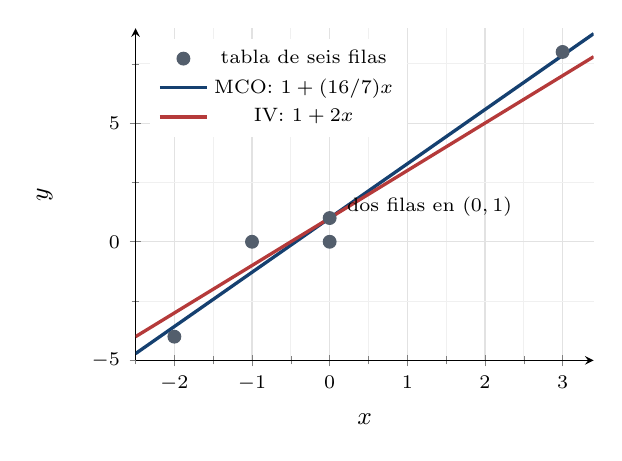
\begin{tikzpicture}\begin{axis}[base,width=7.4cm,height=5.8cm,axis lines=left,xlabel style={at={(axis description cs:.5,-.13)},anchor=north},ylabel style={at={(axis description cs:-.16,.5)},anchor=south,rotate=90},xmin=-2.5,xmax=3.4,ymin=-5,ymax=9,xlabel={$x$},ylabel={$y$},legend pos=north west]
\addplot[only marks,mark=*,mark size=2.3pt,gris]coordinates{(-1,0)(-2,-4)(0,1)(0,0)(3,8)};\addlegendentry{tabla de seis filas}
\addplot[azul,very thick,domain=-2.5:3.4]{1+16*x/7};\addlegendentry{MCO: $1+(16/7)x$}
\addplot[rojo,very thick,domain=-2.5:3.4]{1+2*x};\addlegendentry{IV: $1+2x$}
\node[font=\scriptsize,anchor=west]at(axis cs:.1,1.5){dos filas en $(0,1)$};
\end{axis}\end{tikzpicture}\hfill
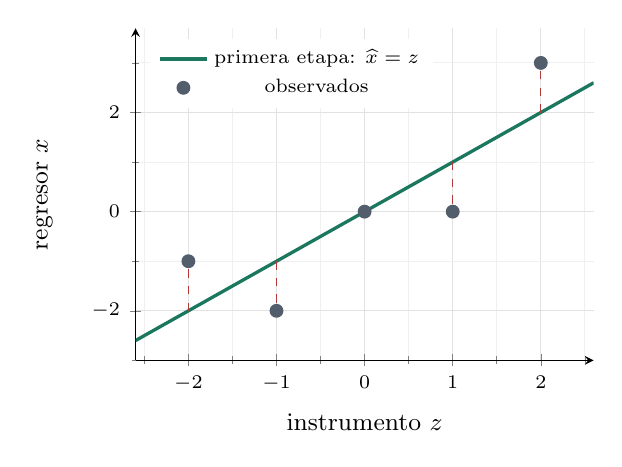
\begin{tikzpicture}\begin{axis}[base,width=7.4cm,height=5.8cm,axis lines=left,xlabel style={at={(axis description cs:.5,-.13)},anchor=north},ylabel style={at={(axis description cs:-.16,.5)},anchor=south,rotate=90},xmin=-2.6,xmax=2.6,ymin=-3,ymax=3.7,xlabel={instrumento $z$},ylabel={regresor $x$},legend pos=north west]
\addplot[verde,very thick,domain=-2.6:2.6]{x};\addlegendentry{primera etapa: $\widehat x=z$}
\addplot[only marks,mark=*,mark size=2.3pt,gris]coordinates{(-2,-1)(-1,-2)(0,0)(1,0)(2,3)};\addlegendentry{observados}
\draw[rojo,dashed](axis cs:-2,-2)--(axis cs:-2,-1);
\draw[rojo,dashed](axis cs:-1,-1)--(axis cs:-1,-2);
\draw[rojo,dashed](axis cs:1,1)--(axis cs:1,0);
\draw[rojo,dashed](axis cs:2,2)--(axis cs:2,3);
\end{axis}\end{tikzpicture}
\caption{Las pendientes MCO e IV difieren en el ejemplo exacto. La primera etapa conserva la parte de $x$ proyectada sobre instrumentos; las líneas verticales representan $v=x-\widehat x$.}
\end{figure}

\subsection{Qué demuestra y qué no demuestra el ejemplo}
Demuestra las multiplicaciones de 2SLS y la diferencia de residuos. Las ortogonalidades de una tabla finita no prueban exogeneidad poblacional. Tampoco la covarianza de IV se conoce con certeza a partir de estos seis números: debe especificarse un modelo probabilístico o utilizar inferencia asintótica válida.

\section{GMM: todos los instrumentos como un problema de optimización}
Define $g_n(b)=n^{-1}Z\T(y-Xb)\in\R^q$ y una matriz de pesos $W\succ0$. Minimizar $g_n(b)\T Wg_n(b)$ da
\[
\widehat\beta_W=(X\T ZWZ\T X)^{-1}X\T ZWZ\T y.
\]
La escala global de $W$ no cambia el estimador. Con $W\propto(Z\T Z)^{-1}$ obtenemos 2SLS. Para un límite $W$ fijo,
\[
V_W=(Q_{xz}WQ_{zx})^{-1}Q_{xz}W\Omega_zWQ_{zx}(Q_{xz}WQ_{zx})^{-1}.
\]
El peso eficiente es $W=\Omega_z^{-1}$ y produce $V_{\rm eficiente}=(Q_{xz}\Omega_z^{-1}Q_{zx})^{-1}$.
\subsection{Por qué ese peso es óptimo: otra prueba de Gauss--Markov}
En el límite, los momentos son una observación normal de media $Q_{zx}h$ y covarianza $\Omega_z$. Entre transformaciones lineales $L$ con $LQ_{zx}=I_p$, la elección
\[
L_*=(Q_{xz}\Omega_z^{-1}Q_{zx})^{-1}Q_{xz}\Omega_z^{-1}
\]
es GLS. Para $L=L_*+D$ con $DQ_{zx}=0$, los términos cruzados se anulan y $L\Omega_zL\T-L_*\Omega_zL_*\T=D\Omega_zD\T\succeq0$. La optimalidad es asintótica dentro de la clase basada en esos momentos.
\subsection{Sobreidentificación y direcciones sobrantes}
Con peso eficiente consistente y las hipótesis regulares,
\[
J=n\,g_n(\widehat\beta)\T\widehat\Omega_z^{-1}g_n(\widehat\beta)
\xrightarrow d\chi^2_{q-p}.
\]
La intuición matricial es que el vector de $q$ momentos blanqueados tiene $p$ direcciones ajustadas por los parámetros y $q-p$ direcciones residuales. Una prueba de sobreidentificación contrasta el conjunto de momentos; no demuestra la validez de cada instrumento individual ni garantiza validez causal.

\parte{X. Support Vector Regression: geometría, dualidad y momentos exactos}
\section{La pérdida insensible y el problema primal de SVR}
En regresión lineal buscamos $f(x)=w\T x+b$. MCO penaliza $r^2$ para el residuo $r=y-f(x)$. SVR usa la pérdida
\[
\ell_\varepsilon(r)=(|r|-\varepsilon)_+=\max(0,r-\varepsilon,-r-\varepsilon),\qquad\varepsilon\ge0.
\]
Los residuos dentro de un tubo de anchura $2\varepsilon$ no generan pérdida. Fuera, el coste crece linealmente. El tubo se mide en unidades de la respuesta, no en una distancia perpendicular al gráfico. La función es convexa por ser máximo de tres funciones afines.
\subsection{Separar ajuste y complejidad}
Con $\phi(x)$ una representación de características en un espacio con producto interno, el problema es
\[
\min_{w,b}\frac12\norm w^2+C\sum_{i=1}^n
\ell_\varepsilon(y_i-\ip w{\phi(x_i)}-b),\qquad C>0.
\]
La norma controla complejidad de $w$; el intercepto no se penaliza. Una escritura equivalente con promedio de pérdida es $\min(\lambda/2)\norm w^2+n^{-1}\sum_i\ell_\varepsilon(r_i)$, con $\lambda=1/(nC)$. El mismo número $C$ bajo convenciones de suma y promedio no representa la misma regularización.
\subsection{Introducir holguras no cambia el objetivo}
Con $\zeta_i,\zeta_i^*\ge0$,
\[
\begin{array}{ll}
\displaystyle\min_{w,b,\zeta,\zeta^*}&\displaystyle\frac12\norm w^2+C\sum_i(\zeta_i+\zeta_i^*)\\[3pt]
\text{sujeto a}& y_i-\ip w{\phi_i}-b\le\varepsilon+\zeta_i,\\
&\ip w{\phi_i}+b-y_i\le\varepsilon+\zeta_i^*,\quad\zeta_i,\zeta_i^*\ge0,
\end{array}
\]
donde $\phi_i=\phi(x_i)$. Para $w,b$ fijos, las holguras mínimas son $(r_i-\varepsilon)_+$ y $(-r_i-\varepsilon)_+$. Su suma es $\ell_\varepsilon(r_i)$. La formulación es una cuadrática convexa con restricciones lineales, incluso cuando $\phi$ tiene muchísimas coordenadas.
\subsection{Existencia y qué parte puede ser no única}
La penalización estrictamente convexa en $w$ obliga a que todos los óptimos tengan el mismo $w$: si dos pendientes distintas fueran óptimas, su punto medio reduciría el término de norma sin aumentar la pérdida convexa. El intercepto puede tener un intervalo de soluciones, porque la pérdida tiene regiones planas. Para hablar de la distribución de un estimador hay que especificar una regla de selección si la solución no es única.
\begin{figure}[H]\centering
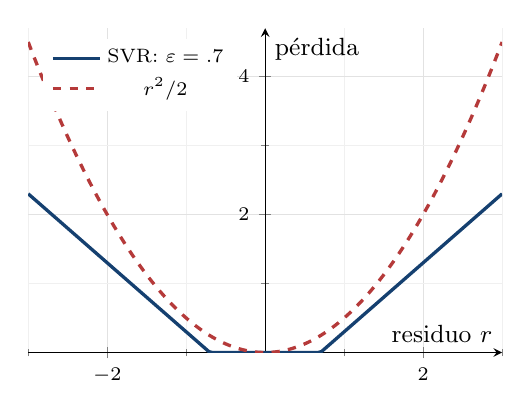
\begin{tikzpicture}\begin{axis}[base,width=7.6cm,height=5.7cm,xmin=-3,xmax=3,ymin=0,ymax=4.7,xlabel={residuo $r$},ylabel={pérdida},legend pos=north west]
\addplot[azul,very thick,domain=-3:3]{max(0,abs(x)-.7)};\addlegendentry{SVR: $\varepsilon=.7$}
\addplot[rojo,dashed,very thick,domain=-3:3]{x*x/2};\addlegendentry{$r^2/2$}
\end{axis}\end{tikzpicture}\hfill
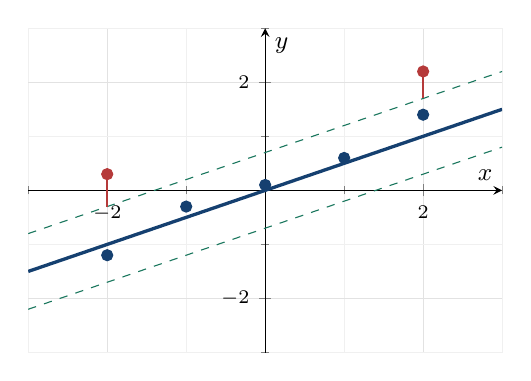
\begin{tikzpicture}\begin{axis}[base,width=7.6cm,height=5.7cm,xmin=-3,xmax=3,ymin=-3,ymax=3,xlabel={$x$},ylabel={$y$}]
\addplot[azul,very thick,domain=-3:3]{.5*x};
\addplot[verde,dashed,domain=-3:3]{.5*x+.7};
\addplot[verde,dashed,domain=-3:3]{.5*x-.7};
\addplot[only marks,mark=*,azul]coordinates{(-2,-1.2)(-1,-.3)(0,.1)(1,.6)(2,1.4)};
\addplot[only marks,mark=*,rojo]coordinates{(-2,.3)(2,2.2)};
\draw[rojo,thick](axis cs:-2,-.3)--(axis cs:-2,.3);
\draw[rojo,thick](axis cs:2,1.7)--(axis cs:2,2.2);
\end{axis}\end{tikzpicture}
\caption{La pérdida ignora una banda central. En el panel geométrico se muestran una función y un tubo ilustrativos; no se afirma que esa recta sea el ajuste óptimo de los puntos dibujados.}
\end{figure}

\section{Dual de SVR: derivar cada multiplicador y cada signo}
Asociamos $\alpha_i,\alpha_i^*\ge0$ a las dos restricciones de residuos y $\eta_i,\eta_i^*\ge0$ a no negatividad de holguras. La Lagrangiana es
\begin{align*}
\mathcal L={}&\frac12\norm w^2+C\sum_i(\zeta_i+\zeta_i^*)\\
&+\sum_i\alpha_i(y_i-\ip w{\phi_i}-b-\varepsilon-\zeta_i)\\
&+\sum_i\alpha_i^*(\ip w{\phi_i}+b-y_i-\varepsilon-\zeta_i^*)
-\sum_i(\eta_i\zeta_i+\eta_i^*\zeta_i^*).
\end{align*}
Las condiciones para el ínfimo respecto a variables primales son
\[
w=\sum_i(\alpha_i-\alpha_i^*)\phi_i,\qquad
\sum_i(\alpha_i-\alpha_i^*)=0,
\]
\[
C-\alpha_i-\eta_i=0,\qquad C-\alpha_i^*-\eta_i^*=0.
\]
Así $0\le\alpha_i,\alpha_i^*\le C$. Sustituir $w$ produce $\tfrac12\norm w^2-\ip w{\sum_i(\alpha_i-\alpha_i^*)\phi_i}=-\tfrac12\norm w^2$. Con $K_{ij}=\ip{\phi_i}{\phi_j}$, el dual es
\[
\boxed{\max_{\alpha,\alpha^*}
y\T(\alpha-\alpha^*)-\varepsilon\ones_n\T(\alpha+\alpha^*)
-\frac12(\alpha-\alpha^*)\T K(\alpha-\alpha^*)}
\]
sujeto a $\ones_n\T(\alpha-\alpha^*)=0$ y las cotas anteriores. Las holguras pueden elegirse estrictamente positivas y suficientemente grandes, así que existe un punto estrictamente factible para las desigualdades: la dualidad fuerte de convexidad se aplica.
\subsection{Una formulación en un solo vector}
Sea $d=\alpha-\alpha^*$. Para un $d_i$ fijo, el menor $\alpha_i+\alpha_i^*$ permitido es $|d_i|$. Si $\varepsilon>0$ el óptimo lo elige; para $\varepsilon=0$ puede haber distintas parejas con el mismo $d$. El dual reducido es
\[
\boxed{\min_{d\in\R^n}\frac12d\T Kd+\varepsilon\norm d_1-y\T d
\quad\text{sujeto a }\ones_n\T d=0,\ -C\le d_i\le C}.
\]
La predicción es $f(x)=\sum_i d_i k(x_i,x)+b$. El problema dual tiene $n$ coordenadas, independientemente del tamaño explícito del espacio de características.
\subsection{KKT y el significado de vector de soporte}
La complementariedad exige
\[
\alpha_i(r_i-\varepsilon-\zeta_i)=0,\quad
\alpha_i^*(-r_i-\varepsilon-\zeta_i^*)=0,
\]
\[
(C-\alpha_i)\zeta_i=0,\qquad(C-\alpha_i^*)\zeta_i^*=0.
\]
Para $\varepsilon>0$:
\begin{center}\small
\begin{tabular}{lll}\toprule
Residuo & Coeficiente dual & Estado\\\midrule
$|r_i|<\varepsilon$ & $d_i=0$ & Interior del tubo.\\
$r_i=\varepsilon$ & $0\le d_i\le C$ & Borde superior de residuo.\\
$r_i>\varepsilon$ & $d_i=C$ & Fuera, holgura positiva.\\
$r_i=-\varepsilon$ & $-C\le d_i\le0$ & Borde inferior de residuo.\\
$r_i<-\varepsilon$ & $d_i=-C$ & Fuera, holgura positiva.\\\bottomrule
\end{tabular}
\end{center}
Un punto con $d_i\ne0$ participa en la expansión y es un vector de soporte. No todos los puntos sobre el borde tienen necesariamente coeficiente no nulo. Si $0<\alpha_i<C$,
\[
b=y_i-\sum_jd_jk(x_j,x_i)-\varepsilon;
\]
si $0<\alpha_i^*<C$, se cambia $-\varepsilon$ por $+\varepsilon$. Si no hay puntos libres, se obtiene un intervalo compatible de $b$ por desigualdades KKT, y debe elegirse una regla dentro de él.

\section{Núcleos y teorema del representante: espacio enorme, cálculo finito}
Un núcleo positivo semidefinido $k$ cumple $\sum_{i,j}c_ic_jk(x_i,x_j)\ge0$ para toda colección finita y todo $c$. Si $k(x,z)=\ip{\phi(x)}{\phi(z)}$, la suma es $\norm{\sum_ic_i\phi(x_i)}^2\ge0$.
\subsection{Por qué no necesitamos una componente perpendicular de $w$}
En un espacio de Hilbert, descomponemos $w=w_\parallel+w_\perp$, donde $w_\parallel$ está en el espacio generado por $\phi_1,\ldots,\phi_n$ y $w_\perp$ es ortogonal a todos. Todas las predicciones de entrenamiento dependen solo de $w_\parallel$, mientras
\[
\norm w^2=\norm{w_\parallel}^2+\norm{w_\perp}^2.
\]
Eliminar $w_\perp$ mantiene la pérdida y reduce penalización. Todo óptimo tiene $w_\perp=0$. Este es el teorema del representante para el problema: incluso con infinitas características basta una combinación de las $n$ observaciones.
\subsection{Núcleo polinómico con características escritas}
Para $x,z\in\R^2$ y $c\ge0$,
\[
k(x,z)=(x\T z+c)^2=\phi(x)\T\phi(z),
\]
\[
\phi(x)=(x_1^2,\sqrt2x_1x_2,x_2^2,\sqrt{2c}x_1,\sqrt{2c}x_2,c)\T.
\]
Multiplicar las seis entradas produce los términos de la expansión del cuadrado. En $p$ variables, las características cuadráticas distintas son $p(p+1)/2$, más $p$ lineales y una constante. Con $p=1000$ ya hay $501501$ características, pero cada producto kernel se calcula con un producto interno de $1000$ entradas.
\subsection{Núcleo gaussiano y expansión infinita}
Para $\gamma>0$,
\begin{align*}
k(x,z)&=e^{-\gamma\norm{x-z}_2^2}\\
&=e^{-\gamma\norm x_2^2}e^{-\gamma\norm z_2^2}
\sum_{m=0}^\infty\frac{(2\gamma)^m}{m!}(x\T z)^m.
\end{align*}
Cada $(x\T z)^m$ es producto interno de tensores $x^{\otimes m},z^{\otimes m}$. Los coeficientes son no negativos; la suma convergente de matrices de Gram positivas semidefinidas sigue siendo positiva semidefinida. Esto demuestra la propiedad del núcleo gaussiano sin construir la lista infinita de características.
\subsection{Escalado y coste en dimensión grande}
Si una variable se multiplica por $100$, su contribución a $\norm{x-z}_2^2$ se multiplica por $10000$ y puede dominar un núcleo gaussiano. Estandarización, Mahalanobis y elección de $\gamma$ forman parte del modelo. $K$ requiere $n^2$ entradas: con $n=10000$, son $10^8$ números. El truco kernel elimina la dimensión explícita de características, pero no elimina todo coste de muestra.

\section{SVR con dos puntos: solución exacta, primal y dual}
Sean $x_1=-1$, $x_2=1$, $y_1=-a$, $y_2=a$, $a>0$. Por simetría podemos elegir $b=0$, y un óptimo tiene $w\ge0$. La función a minimizar se reduce a
\[
J(w)=\frac12w^2+2C(a-w-\varepsilon)_+.
\]
Si $a\le\varepsilon$, $w=0$ da pérdida y penalización cero. Si $a>\varepsilon$, en $0\le w<a-\varepsilon$ la derivada es $w-2C$; en $w>a-\varepsilon$ es $w$. Por tanto
\[
\boxed{w_* =\min\{(a-\varepsilon)_+,2C\},\qquad b_*=0}.
\]
El caso general con $y_1,y_2$ sustituye $a$ por el contraste $D=(y_2-y_1)/2$, permitiendo signo, y elige $b=(y_1+y_2)/2$:
\[
w_* =\operatorname{clip}\!\left(\operatorname{soft}_\varepsilon(D),-2C,2C\right).
\]
Para verlo, el intercepto medio deja residuos opuestos $D-w$ y $-(D-w)$ y minimiza su suma de pérdidas por convexidad y simetría. La solución en $w$ se deduce por los mismos casos.
\subsection{Ejemplo con borde libre}
Con $a=2$, $\varepsilon=1/2$, $C=1$, $w=3/2$, los residuos son $(-1/2,1/2)$. El dual usa $d=(-3/4,3/4)\T$:
\[
K=\begin{pmatrix}1&-1\\-1&1\end{pmatrix},\quad
\sum_id_ix_i=3/2,\quad\ones_2\T d=0,\quad|d_i|<C.
\]
El objetivo primal es $\tfrac12(3/2)^2=9/8$. El valor dual es $y\T d-\varepsilon\norm d_1-\tfrac12d\T Kd=3-3/4-9/8=9/8$. Igualdad de valores y KKT certifican el óptimo.
\subsection{Ejemplo con saturación}
Con los mismos $a,\varepsilon$, pero $C=1/4$, $w=1/2$ y $d=(-1/4,1/4)\T$. Cada holgura vale uno. La función acepta error fuera del tubo para reducir pendiente:
\[
J=\frac12(1/2)^2+\frac14(1+1)=\frac58.
\]
No existe la identidad $w=(X\T X)^{-1}X\T y$ en SVR: aparece un umbral y una saturación, aunque el modelo de predicción siga siendo lineal.

\section{Esperanza, varianza y covarianza exactas de una SVR gaussiana}
Usamos el ejemplo de dos diseños fijos $x_1=-1,x_2=1$, pero respuestas aleatorias
\[
y_i=b_0+\beta x_i+u_i,\qquad u_1,u_2\ \text{independientes},\quad u_i\sim\mathcal N(0,\sigma^2).
\]
Fijamos $C>0$, $\varepsilon\ge0$ y la selección del intercepto $\widehat b=(y_1+y_2)/2$. Sean
\[
D=(y_2-y_1)/2\sim\mathcal N(\beta,s^2),\quad s^2=\sigma^2/2,
\qquad\widehat b\sim\mathcal N(b_0,s^2).
\]
Son independientes porque son combinaciones gaussianas de covarianza cero. La pendiente es $\widehat w=T(D)$, con $M=2C$ y
\[
T(d)=\begin{cases}
-M,&d<-\varepsilon-M,\\
d+\varepsilon,&-\varepsilon-M\le d<-\varepsilon,\\
0,&|d|\le\varepsilon,\\
d-\varepsilon,&\varepsilon<d\le\varepsilon+M,\\
M,&d>\varepsilon+M.
\end{cases}
\]

\begin{figure}[H]\centering
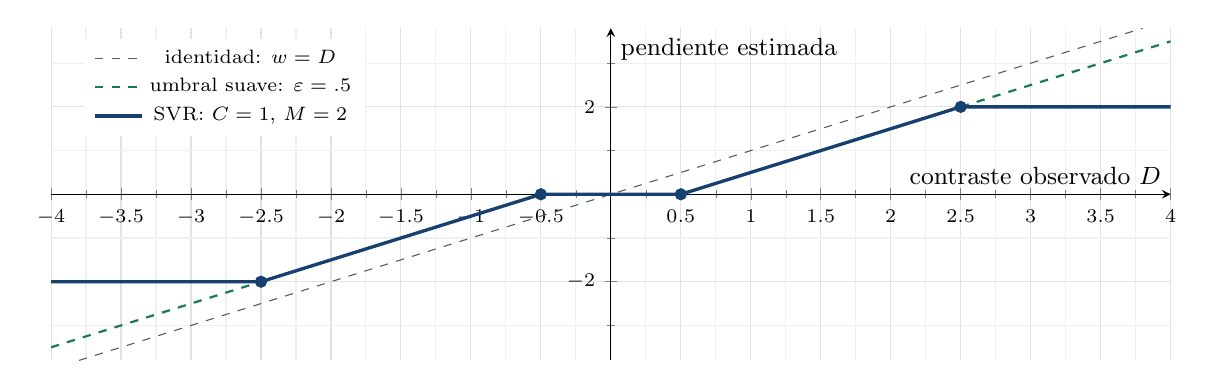
\begin{tikzpicture}\begin{axis}[base,width=15.8cm,height=5.8cm,xmin=-4,xmax=4,ymin=-3.8,ymax=3.8,xlabel={contraste observado $D$},ylabel={pendiente estimada},legend pos=north west]
\addplot[gris,dashed,domain=-3.8:3.8]{x};\addlegendentry{identidad: $w=D$}
\addplot[verde,dashed,thick]coordinates{(-4,-3.5)(-.5,0)(.5,0)(4,3.5)};\addlegendentry{umbral suave: $\varepsilon=.5$}
\addplot[azul,very thick]coordinates{(-4,-2)(-2.5,-2)(-.5,0)(.5,0)(2.5,2)(4,2)};\addlegendentry{SVR: $C=1$, $M=2$}
\addplot[only marks,mark=*,azul]coordinates{(-2.5,-2)(-.5,0)(.5,0)(2.5,2)};
\end{axis}\end{tikzpicture}
\caption{La transformación exacta de la SVR de dos puntos tiene umbral y saturación. Intervalos completos de $D$ se convierten en un único valor de $\widehat w$, generando átomos de probabilidad.}
\end{figure}

\subsection{La distribución contiene masas puntuales}
Sea $F(t)=\Phi((t-\beta)/s)$. Hay probabilidad $F(\varepsilon)-F(-\varepsilon)$ en cero, $F(-\varepsilon-M)$ en $-M$ y $1-F(\varepsilon+M)$ en $M$. En $0<w<M$, la densidad es $f_D(w+\varepsilon)$; en $-M<w<0$, es $f_D(w-\varepsilon)$. El estimador no es normal: una distribución normal no tiene esas masas puntuales.
\subsection{Momentos de una normal truncada, deducidos por integración}
Para $L<U$, define $z_L=(L-\beta)/s$, $z_U=(U-\beta)/s$ y
\[
P(L,U)=F(U)-F(L),\quad J_k(L,U)=\int_L^U d^k f_D(d)\dd d.
\]
Como $\int z\phi(z)\dd z=-\phi(z)$ y $\int z^2\phi(z)\dd z=\Phi(z)-z\phi(z)$,
\[
J_1=\beta P+s[\phi(z_L)-\phi(z_U)],
\]
\[
J_2=(\beta^2+s^2)P+2\beta s[\phi(z_L)-\phi(z_U)]
+s^2[z_L\phi(z_L)-z_U\phi(z_U)].
\]
Estos son momentos \emph{sin normalizar}: no son la media condicionada al intervalo, que sería $J_1/P$.
\subsection{Integrar los cinco tramos da los momentos exactos}
Escribe $I_-=(-\varepsilon-M,-\varepsilon)$, $I_+=(\varepsilon,\varepsilon+M)$; en $P_\pm,J_{k,\pm}$ se usan esos límites. Entonces
\begin{align*}
\E\widehat w={}&J_{1,-}+\varepsilon P_-+J_{1,+}-\varepsilon P_+\\
&+M[1-F(\varepsilon+M)-F(-\varepsilon-M)],
\end{align*}
\begin{align*}
\E\widehat w^2={}&J_{2,-}+2\varepsilon J_{1,-}+\varepsilon^2P_-\\
&+J_{2,+}-2\varepsilon J_{1,+}+\varepsilon^2P_+\\
&+M^2[F(-\varepsilon-M)+1-F(\varepsilon+M)].
\end{align*}
Por tanto el sesgo de pendiente es $\E\widehat w-\beta$ y su varianza $\E\widehat w^2-(\E\widehat w)^2$. La matriz de todos los momentos de los dos coeficientes es
\[
\boxed{\E\begin{pmatrix}\widehat b\\\widehat w\end{pmatrix}
=\begin{pmatrix}b_0\\\E\widehat w\end{pmatrix},\qquad
\Cov\begin{pmatrix}\widehat b\\\widehat w\end{pmatrix}
=\begin{pmatrix}s^2&0\\0&\Var(\widehat w)\end{pmatrix}}.
\]
La covarianza cero se debe aquí a independencia exacta entre media y contraste; no es una propiedad general de SVR. Si $\beta=0$, simetría implica $\E\widehat w=0$. Para $\beta\ne0$, el umbral y saturación suelen producir sesgo hacia cero.
\subsection{Momentos de todas las predicciones}
Con $\widehat f(x)=\widehat b+x\widehat w$,
\[
\E\widehat f(x)=b_0+x\E\widehat w,
\quad\Cov(\widehat f(x),\widehat f(z))=s^2+xz\Var(\widehat w).
\]
El error cuadrático de estimar la media verdadera $b_0+\beta x$ es $s^2+x^2\Var(\widehat w)+x^2(\E\widehat w-\beta)^2$. Para predecir una observación nueva independiente se añade $\sigma^2$. Tenemos fórmulas exactas porque especificamos diseño, distribución, hiperparámetros y selección de solución.

\section{SVR general: regiones activas, Jacobiano local e incertidumbre}
Para un kernel fijo, $C,\varepsilon$ fijos y respuestas $y$ variables, el dual reducido es una optimización cuadrática con términos por tramos. Supón que un conjunto $S$ de coeficientes duales satisface $0<|d_i|<C$, con signos $s_i$ fijos. Los restantes $d_T$ están fijos en $0$ o en $\pm C$. Dentro de una región sin cambios de estado, KKT da
\[
\begin{pmatrix}K_{SS}&\ones_S\\\ones_S\T&0\end{pmatrix}
\begin{pmatrix}d_S\\b\end{pmatrix}
=\begin{pmatrix}y_S-K_{ST}d_T-\varepsilon s_S\\-\ones_T\T d_T\end{pmatrix}.
\]
Si el bloque es invertible, $(d_S,b)$ es una función afín de $y_S$ en esa región. Su diferencial cumple
\[
\begin{pmatrix}\mathrm dd_S\\\mathrm db\end{pmatrix}
=\begin{pmatrix}K_{SS}&\ones_S\\\ones_S\T&0\end{pmatrix}^{-1}
\begin{pmatrix}\mathrm dy_S\\0\end{pmatrix}.
\]
Esto permite estudiar sensibilidad \emph{local}. Al cruzar un borde cambia el conjunto activo y cambia el Jacobiano. Una única matriz de diseño inversa no describe la distribución global.
\subsection{Momentos globales como integrales sobre regiones}
Para una selección determinada del óptimo, sea $\theta(y)$ el vector de coeficientes o predicciones. Si en una región $\mathcal R$ vale $\theta=A_{\mathcal R}y+c_{\mathcal R}$,
\[
\E\theta=\sum_{\mathcal R}\Prob(y\in\mathcal R)
\left[A_{\mathcal R}\E(y\mid\mathcal R)+c_{\mathcal R}\right],
\]
\[
\Cov(\theta)=\sum_{\mathcal R}\Prob(\mathcal R)
\left[A_{\mathcal R}\Cov(y\mid\mathcal R)A_{\mathcal R}\T
+(m_{\mathcal R}-m)(m_{\mathcal R}-m)\T\right].
\]
Son identidades exactas cuando los momentos existen. Condicionar a una región activa trunca la distribución de $y$; no se debe sustituir $\Cov(y\mid\mathcal R)$ por la covarianza no condicionada sin justificación.
\subsection{Por qué no hay una covarianza universal de SVR}
La respuesta depende de la distribución de datos, kernel, $C$, $\varepsilon$, reglas de selección y, si se ajustan hiperparámetros, de ese procedimiento. El bootstrap que reentrena puede estudiar incertidumbre bajo un esquema especificado, pero no convierte SVR en MCO normal. El caso de dos puntos muestra explícitamente cómo se calculan los momentos sin inventar una fórmula lineal que el algoritmo no tiene.

\parte{XI. Aprendizaje automático y econometría: qué aporta PCA}
\section{PCA frente a regresión: proyecciones en espacios distintos}
Para regresión lineal centrada, $y_c\in\R^{n\times1}$ es una respuesta y $X_c\in\R^{n\times p}$ contiene predictores. MCO busca
\[
\min_{\beta\in\R^{p\times1}}\norm{y_c-X_c\beta}_2^2,
\qquad X_c\T X_c\widehat\beta=X_c\T y_c.
\]
Si $X_c$ tiene rango columna completo, $\widehat\beta=(X_c\T X_c)^{-1}X_c\T y_c$. En cambio, PCA no recibe $y_c$ y busca aproximar $X_c$ mismo.
\subsection{Dos operadores de proyección que no deben confundirse}
Con la SVD compacta $X_c=U_rD_rV_r\T$,
\[
P_{\mathrm{obs}}=U_rU_r\T\in\R^{n\times n},\qquad
P_{\mathrm{var}}=V_kV_k\T\in\R^{p\times p}.
\]
MCO proyecta $y_c$ en el espacio columna de $X_c$: $\widehat y_c=P_{\mathrm{obs}}y_c$. PCA proyecta las \emph{filas} de $X_c$ en un subespacio del espacio de variables: $\widehat X_c=X_cP_{\mathrm{var}}$. Las dimensiones revelan la diferencia.
\subsection{Regresión vertical frente a distancia perpendicular}
Si una nube bidimensional tiene covarianza $S=\begin{psmallmatrix}a&b\\b&c\end{psmallmatrix}$, con $a>0$, la pendiente de la regresión de la segunda variable sobre la primera es $b/a$. La pendiente de la primera componente, cuando $v_{11}\ne0$, es $v_{21}/v_{11}$, obtenida por el autovector dominante. Para el ejemplo maestro,
\[
\text{pendiente MCO}=\frac{4}{28/5}=\frac57,\qquad
\text{pendiente PCA}=1.
\]
MCO minimiza errores verticales en una variable designada como respuesta; PCA minimiza distancias perpendiculares tratando ambas variables simétricamente dentro de la métrica elegida.
\begin{figure}[H]\centering
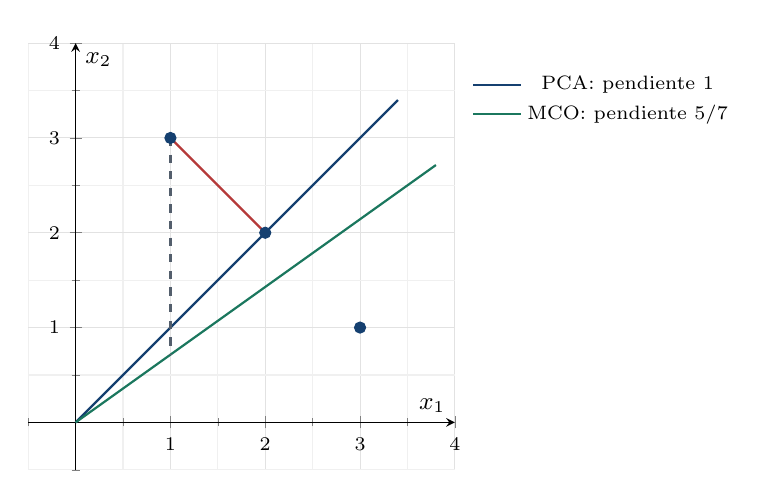
\begin{tikzpicture}
\begin{axis}[base,width=10cm,height=7cm,axis equal image,xmin=-.5,xmax=4,ymin=-.5,ymax=4,xlabel={$x_1$},ylabel={$x_2$},legend style={at={(1.02,.95)},anchor=north west}]
\addplot[azul,thick,domain=0:3.4]{x};\addlegendentry{PCA: pendiente 1}
\addplot[verde,thick,domain=0:3.8]{5*x/7};\addlegendentry{MCO: pendiente $5/7$}
\addplot[only marks,mark=*,azul]coordinates{(1,3)(2,2)(3,1)};
\draw[rojo,thick](axis cs:1,3)--(axis cs:2,2);
\draw[gris,dashed,thick](axis cs:1,3)--(axis cs:1,.714286);
\end{axis}\end{tikzpicture}
\caption{Se muestran los tres puntos positivos del ejemplo maestro. El segmento rojo es perpendicular a la recta PCA; el gris mide el error vertical para MCO.}
\end{figure}

\section{Regresión por componentes principales: deducción y sesgo}
En PCR se conserva $Z_k=X_cV_k=U_kD_k\in\R^{n\times k}$ y se ajusta
\[
y_c=Z_k\gamma+\varepsilon,\qquad \gamma\in\R^{k\times1},\quad\varepsilon\in\R^{n\times1}.
\]
Como $Z_k\T Z_k=D_k^2$,
\[
\widehat\gamma=(Z_k\T Z_k)^{-1}Z_k\T y_c=D_k^{-1}U_k\T y_c,
\]
\[
\boxed{\widehat\beta_{\mathrm{PCR},k}=V_kD_k^{-1}U_k\T y_c\in\R^{p\times1}},\qquad
\widehat y_c=U_kU_k\T y_c.
\]
El intercepto recuperado es $\widehat\beta_0=\bar y-\bar x\T\widehat\beta_{\mathrm{PCR},k}$. Usar todas las componentes de rango positivo produce la solución MCO de mínima norma, incluso si $p>n$.
\subsection{Descomposición de sesgo y varianza condicional}
Supón $y_c=X_c\beta+\varepsilon$ en el espacio centrado, con ruido original homocedástico de varianza $\sigma^2$; en las direcciones de $U_r$, su covarianza sigue siendo $\sigma^2I_r$. Fijado $X_c$,
\[
\E[\widehat\beta_{\mathrm{PCR},k}\mid X_c]=V_kV_k\T\beta,\qquad
\Cov(\widehat\beta_{\mathrm{PCR},k}\mid X_c)=\sigma^2V_kD_k^{-2}V_k\T.
\]
Escribe $\beta=\sum_{j=1}^p b_jv_j$, con $b_j=v_j\T\beta$. Entonces
\[
\E[\norm{\widehat\beta_{\mathrm{PCR},k}-\beta}_2^2\mid X_c]
=\sum_{j=k+1}^pb_j^2+\sigma^2\sum_{j=1}^k\frac1{d_j^2}.
\]
Se reduce varianza al evitar dividir por valores singulares pequeños, pero se introduce sesgo si $\beta$ tiene componentes en ejes descartados. Para predecir en el diseño observado,
\[
\E[\norm{X_c\widehat\beta_{\mathrm{PCR},k}-X_c\beta}_2^2\mid X_c]
=\sum_{j=k+1}^rd_j^2b_j^2+\sigma^2k.
\]
Estas expresiones separan error de estimación de coeficientes y error de predicción; no son intercambiables.
\begin{ejemplo}[Una señal importante puede tener varianza pequeña]
Sean variables independientes $\xi_1\sim N(0,100)$ y $\xi_2\sim N(0,0.01)$, con respuesta $Y=10\xi_2$. PCA conserva primero $\xi_1$, que explica $100/100.01\approx99.990\%$ de la varianza de predictores. Pero $Y$ depende solo de la segunda variable. Usando solo la primera, el mejor predictor cuadrático es $\E[Y\mid\xi_1]=0$ y su error es $\Var(Y)=1$. Conservando la segunda, la predicción es exacta. Mucha varianza explicada en $X$ no asegura buena predicción de $Y$.
\end{ejemplo}

\section{Ridge, pseudoinversa y filtros espectrales}
Ridge resuelve, para $\alpha>0$,
\[
\min_{\beta\in\R^{p\times1}}\norm{y_c-X_c\beta}_2^2+\alpha\norm\beta_2^2,
\qquad\widehat\beta_{\mathrm{ridge}}=(X_c\T X_c+\alpha I_p)^{-1}X_c\T y_c.
\]
Sustituyendo la SVD,
\[
\widehat\beta_{\mathrm{ridge}}=\sum_{j=1}^r\frac{d_j}{d_j^2+\alpha}v_ju_j\T y_c,
\qquad
\widehat y_c=\sum_{j=1}^r\frac{d_j^2}{d_j^2+\alpha}u_ju_j\T y_c.
\]
La pseudoinversa de $X_c$ es $X_c^+=V_rD_r^{-1}U_r\T\in\R^{p\times n}$, y la solución MCO de mínima norma es $X_c^+y_c$.
\begin{center}\small
\begin{tabular}{lll}\toprule
Método & Factor sobre $u_ju_j\T y_c$ & Acción\\\midrule
MCO de mínima norma & $1$ para $d_j>0$ & Conserva toda dirección identificable\\
PCR con $k$ & $\ind_{\{j\le k\}}$ & Corte abrupto de direcciones\\
Ridge & $d_j^2/(d_j^2+\alpha)$ & Atenuación continua\\\bottomrule
\end{tabular}\end{center}
\subsection{Ejemplo numérico de la atenuación}
Si $d_1^2=48$, $d_2^2=8$ y $\alpha=8$, los factores de predicción ridge son $48/56=6/7$ y $8/16=1/2$. PCR con $k=1$ usa $1$ y $0$. No son el mismo procedimiento: ambos controlan direcciones poco estables, pero hacen compromisos diferentes.
\subsection{El número efectivo de parámetros}
Para ridge, la matriz suavizadora es $H_\alpha=U_r\diag(d_j^2/(d_j^2+\alpha))U_r\T\in\R^{n\times n}$ y
\[
\operatorname{df}_{\mathrm{ridge}}=\tr(H_\alpha)=\sum_{j=1}^r\frac{d_j^2}{d_j^2+\alpha}.
\]
Para PCR con ejes y $k$ fijos, $\tr(U_kU_k\T)=k$. Si $k$ se selecciona utilizando la respuesta, la complejidad total de la selección no queda completamente descrita por ese $k$.

\section{PCA dentro de un flujo de aprendizaje automático}
\subsection{Entrenar, transformar y evaluar sin fuga de información}
El conjunto de entrenamiento determina $\bar x$, las escalas $D$, los ejes $V_k$ y cualquier elección de $k$. En validación se aplica
\[
z_{\mathrm{val}}=V_k\T D^{-1}(x_{\mathrm{val}}-\bar x)\in\R^{k\times1},
\]
con $D=I_p$ si no se estandariza. Ajustar PCA antes de separar validación utiliza la distribución de los datos que se pretende evaluar; puede contaminar la evaluación aunque PCA no use etiquetas. En validación cruzada se repite todo el ajuste dentro de cada partición.
\subsection{Clasificación, agrupamiento y detección de anomalías}
Un clasificador puede usar $z_i$ como entrada; por ejemplo, en una regresión logística,
\[
\Pr(Y_i=1\mid z_i)=\frac1{1+\exp[-(\beta_0+\gamma\T z_i)]},\qquad
\gamma\in\R^{k\times1}.
\]
En coordenadas originales, el coeficiente es $D^{-1}V_k\gamma\in\R^{p\times1}$. La restricción a ese subespacio puede mejorar estabilidad o eliminar señal predictiva; se decide con evaluación supervisada.

En agrupamiento, las distancias entre puntuaciones pueden eliminar ruido, pero también borrar grupos diferenciados en direcciones de baja varianza. Para anomalías conviene distinguir
\[
T_i^2=z_i\T\Lambda_k^{-1}z_i,\qquad
Q_i=\norm{(I_p-P_k)(x_i-\bar x)}_2^2.
\]
$T_i^2$ detecta puntuaciones extremas dentro del subespacio; $Q_i$ detecta desviaciones fuera de él. Sus umbrales estadísticos requieren un modelo y un esquema de estimación; no se toma automáticamente una distribución chi-cuadrado para ambos.
\subsection{Datos faltantes, valores atípicos y variables categóricas}
PCA ordinario requiere una matriz numérica completa. Imputar con medias puede reducir artificialmente varianza y covarianza. Una alternativa es ajustar rango bajo usando solo entradas observadas; otra es un modelo probabilístico. Los atípicos pueden dominar la covarianza porque las desviaciones se elevan al cuadrado. Las variables categóricas codificadas como enteros no adquieren una distancia cuantitativa válida por el mero hecho de tener números; puede ser necesario otro tipo de representación o análisis.
\begin{cuidado}[Interpretación y causalidad]
Una componente explica dispersión, no causas. Un eje con cargas altas en ingreso, educación y consumo puede resumir una asociación, pero no identifica un efecto causal ni una variable latente única. Su nombre es una interpretación sustantiva que debe contrastarse con el diseño y las variables.
\end{cuidado}

\section{Autoencoders lineales: por qué reaparece el subespacio PCA}
Un autoencoder lineal centrado usa un codificador $B\in\R^{p\times k}$ y un decodificador $C\in\R^{k\times p}$:
\[
Z=X_cB\in\R^{n\times k},\qquad\widehat X_c=X_cBC\in\R^{n\times p},\qquad
\min_{B,C}\norm{X_c-X_cBC}\F^2.
\]
Como $\rank(X_cBC)\le k$, el teorema de mejor aproximación impone un error al menos $\sum_{j>k}d_j^2$. Se alcanza con $B=V_k$ y $C=V_k\T$; por tanto el mínimo global coincide con PCA.
\subsection{El código latente no tiene que ser una componente principal}
Para cualquier matriz invertible $R\in\R^{k\times k}$,
\[
B=V_kR,\qquad C=R^{-1}V_k\T\quad\Rightarrow\quad BC=V_kV_k\T.
\]
La reconstrucción es la misma, pero el código $X_cV_kR$ puede tener coordenadas correlacionadas, escalas distintas y ejes no ortogonales. Coincidir en subespacio óptimo no implica recuperar individualmente los autovectores. Con no linealidades, regularización o pérdidas diferentes, el problema deja de ser PCA en general.
\subsection{Un cuello de botella no prueba una estructura causal}
Una representación que reconstruye bien puede mezclar factores interpretables de muchas maneras. Identificar factores o mecanismos necesita restricciones adicionales; el tamaño $k$ del código, por sí solo, no proporciona esa identificación.

\section{PCA probabilístico: variables latentes y ruido isotrópico}
En PPCA se postula, para cada observación aleatoria $\xi\in\R^{p\times1}$,
\[
\xi=\mu+Wh+\varepsilon,\quad
h\sim N_k(0,I_k),\quad\varepsilon\sim N_p(0,\sigma^2I_p),\quad h\perp\!\!\!\perp\varepsilon,
\]
con $W\in\R^{p\times k}$, $\mu\in\R^{p\times1}$ y $\sigma^2>0$. Integrando $h$,
\[
\xi\sim N_p(\mu,C),\qquad C=WW\T+\sigma^2I_p\in\R^{p\times p}.
\]
El ruido tiene la misma varianza en todas las direcciones; es una hipótesis fuerte, distinta de exigir simplemente segundos momentos.
\subsection{Verosimilitud y estimación de la media}
Para observaciones independientes, omitiendo constantes,
\[
\ell(\mu,W,\sigma^2)=-\frac n2\log\det C
-\frac12\sum_i(x_i-\mu)\T C^{-1}(x_i-\mu).
\]
Derivar respecto a $\mu$ da $C^{-1}\sum_i(x_i-\mu)=0$, así que $\widehat\mu=\bar x$. Con $S_n=X_c\T X_c/n$,
\[
\ell=-\frac n2\left[\log\det C+\tr(C^{-1}S_n)\right]+\text{constante}.
\]
Aquí los autovalores relevantes son $\ell_1\ge\cdots\ge\ell_p\ge0$ de $S_n$, no los de $S$; $\ell_j=(n-1)\lambda_j/n$.
\subsection{Solución espectral y origen de la varianza de ruido}
Para $k<p$, en el caso interior no degenerado,
\[
\widehat\sigma^2=\frac1{p-k}\sum_{j=k+1}^p\ell_j,\qquad
\widehat W=V_k(\operatorname{diag}(\ell_1,\ldots,\ell_k)-\widehat\sigma^2I_k)^{1/2}R,
\]
con $R\in\R^{k\times k}$ ortogonal. La solución exige $\ell_j\ge\widehat\sigma^2$ en los ejes retenidos; si hay igualdades, algunas cargas se anulan. Si el promedio residual es cero, el óptimo puede estar en la frontera $\sigma^2=0$, donde la densidad no degenerada requiere tratamiento límite.
\begin{deduccion}
Fijados los autovalores de $C$, el término $\log\det C$ no depende de sus ejes. La traza $\tr(C^{-1}S_n)$ se minimiza alineando mayores autovalores de $S_n$ con mayores autovalores de $C$: si dos pares están invertidos, el cambio de coste al intercambiarlos es
\[
\frac{\ell_a}{c_a}+\frac{\ell_b}{c_b}-\frac{\ell_a}{c_b}-\frac{\ell_b}{c_a}
=(\ell_a-\ell_b)(c_a^{-1}-c_b^{-1})\le0
\]
cuando $\ell_a\ge\ell_b$ y $c_a\ge c_b$. La extensión a bases ortogonales se obtiene porque los cuadrados de los productos entre ejes forman una matriz doblemente estocástica y la traza es lineal en esos pesos. El mínimo está en una alineación de ejes.

En los $k$ ejes de señal, $c_j=\sigma^2+\omega_j^2$; en los restantes, $c_j=\sigma^2$. El objetivo escalar es
\[
\sum_{j=1}^k\left(\log c_j+\frac{\ell_j}{c_j}\right)
+(p-k)\log\sigma^2+\frac{\sum_{j>k}\ell_j}{\sigma^2}.
\]
Derivar $\log c+\ell/c$ da $(c-\ell)/c^2$; el mínimo es $c_j=\ell_j$ para ejes activos. Derivar respecto a $s=\sigma^2$ en el bloque restante da $(p-k)/s-\sum_{j>k}\ell_j/s^2=0$, de donde el promedio residual. Finalmente $WW\T=V_k\diag(\ell_j-\widehat\sigma^2)V_k\T$ permite cualquier rotación latente $R$.
\end{deduccion}
\subsection{Distribución posterior del factor latente: completar cuadrados}
Define $M=W\T W+\sigma^2I_k\in\R^{k\times k}$ y $y=x-\mu\in\R^{p\times1}$. La densidad condicional de $h$ es proporcional a
\[
\exp\left[-\frac12h\T h-\frac1{2\sigma^2}(y-Wh)\T(y-Wh)\right].
\]
Al agrupar términos en $h$,
\[
h\T Mh-2h\T W\T y
=(h-M^{-1}W\T y)\T M(h-M^{-1}W\T y)-y\T WM^{-1}W\T y.
\]
Por tanto,
\[
\boxed{h\mid x\sim N_k(M^{-1}W\T(x-\mu),\ \sigma^2M^{-1})}.
\]
El código posterior encoge y escala las puntuaciones; no es simplemente $V_k\T(x-\mu)$. PPCA permite cuantificar incertidumbre latente y tratar datos incompletos dentro de un modelo. La formulación probabilística clásica se debe a Tipping y Bishop; su artículo se incluye en las referencias.
\subsection{PCA frente a análisis factorial}
En análisis factorial, $\Cov(\varepsilon)=\Psi$ suele ser diagonal con entradas diferentes; entonces $C=WW\T+\Psi$. Esto distingue variación específica por variable de variación común. PCA descompone varianza total sin ese modelo; PPCA es un modelo particular con $\Psi=\sigma^2I_p$. Las tres formulaciones no deben usarse como sinónimos.

\parte{XII. Portafolios: la conexión precisa con autovectores y PCA}
\section{Retornos, pesos y varianza como forma cuadrática}
Sea $R=(R_1,\ldots,R_p)\T\in\R^{p\times1}$ un vector aleatorio de retornos, $\mu=\E[R]\in\R^{p\times1}$ y $\Sigma=\Cov(R)\in\R^{p\times p}$. Un vector de pesos $w=(w_1,\ldots,w_p)\T\in\R^{p\times1}$ produce
\[
R_P=w\T R=\sum_jw_jR_j,\quad
\mu_P=w\T\mu,\quad
\sigma_P^2=\Var(w\T R)=w\T\Sigma w.
\]
Con presupuesto total invertido, $\ones_p\T w=1$. Si se prohíben posiciones cortas, además $w_j\ge0$. Un peso negativo significa una posición corta dentro del modelo; no es un error algebraico, aunque puede estar excluido por la aplicación.
\subsection{Expansión para dos activos}
Con $w=(a,1-a)\T$, desviaciones $\sigma_1,\sigma_2$ y correlación $\rho$,
\[
\Sigma=\begin{pmatrix}\sigma_1^2&\rho\sigma_1\sigma_2\\\rho\sigma_1\sigma_2&\sigma_2^2\end{pmatrix},\quad
\sigma_P^2=a^2\sigma_1^2+(1-a)^2\sigma_2^2+2a(1-a)\rho\sigma_1\sigma_2.
\]
La diversificación procede del término de covarianza. No basta contar activos: si se mueven de manera casi idéntica, la reducción de riesgo puede ser limitada.
\begin{ejemplo}[Dos activos con riesgo y correlación distintos]
Tomemos datos hipotéticos, en una misma unidad temporal:
\[
\mu=(0.08,0.14)\T,\quad
\Sigma=\begin{pmatrix}0.04&0.006\\0.006&0.09\end{pmatrix},\quad
\sigma_1=0.20,\quad\sigma_2=0.30,\quad\rho=0.10.
\]
Para $w=(1/2,1/2)\T$,
\[
\mu_P=0.11,\qquad \sigma_P^2=0.25(0.04)+0.25(0.09)+0.5(0.006)=0.0355,
\quad\sigma_P\approx0.188414.
\]
La desviación del portafolio es menor que la de cualquiera de los dos activos en este ejemplo. Todos los valores son ilustrativos; no son cotizaciones ni estimaciones de una inversión real.
\end{ejemplo}

\section{Cuándo el portafolio sí lleva a una ecuación propia}
Consideremos primero un problema geométrico de exposición con \emph{norma} fija:
\[
\min_{w\T w=1}w\T\Sigma w\qquad\text{o}\qquad
\max_{w\T w=1}w\T\Sigma w.
\]
Su lagrangiano es $\mathcal L=w\T\Sigma w-\lambda(w\T w-1)$, por lo que
\[
2\Sigma w-2\lambda w=0\quad\Longleftrightarrow\quad
\boxed{\Sigma w=\lambda w}.
\]
El mínimo se alcanza en el autoespacio de $\lambda_p$ y el máximo en el de $\lambda_1$. El problema de PCA es el de \emph{máxima} varianza con esta normalización.
\subsection{La restricción determina el lado derecho}
Con presupuesto, el problema es $\min w\T\Sigma w$ sujeto a $\ones_p\T w=1$. Ahora
\[
\mathcal L=w\T\Sigma w-2\eta(\ones_p\T w-1),\qquad
2\Sigma w-2\eta\ones_p=0,
\]
\[
\boxed{\Sigma w=\eta\ones_p}.
\]
El lado derecho es el vector de unos, no $w$. Se parece a una ecuación propia porque ambas surgen de formas cuadráticas, pero la derivada de la restricción cambió.
\begin{center}\small
\begin{tabular}{>{\raggedright\arraybackslash}p{4.2cm}>{\raggedright\arraybackslash}p{5.2cm}>{\raggedright\arraybackslash}p{5.6cm}}\toprule
Restricción & Condición de primer orden & Interpretación\\\midrule
$w\T w=1$ & $\Sigma w=\lambda w$ & Autovector ordinario; riesgo por norma\\
$\ones_p\T w=1$ & $\Sigma w=\eta\ones_p$ & Portafolio con presupuesto\\
$w\T Bw=1$, $B\succ0$ & $\Sigma w=\lambda Bw$ & Autovector generalizado\\
$\ones_p\T w=1$, $\mu\T w=m$ & $\Sigma w=\eta\ones_p+\gamma\mu$ & Riesgo mínimo para retorno fijado\\\bottomrule
\end{tabular}\end{center}
\begin{cuidado}[Normalizar un autovector no resuelve automáticamente Markowitz]
Si $v$ es un autovector y $\ones_p\T v\ne0$, podemos imponer presupuesto con $w=v/(\ones_p\T v)$. Eso vuelve factible el vector, pero no garantiza optimalidad de mínima varianza con presupuesto. Si $\ones_p\T v=0$, ni siquiera se puede hacer esa normalización: es una exposición de inversión neta cero.
\end{cuidado}

\section{Portafolio global de mínima varianza: solución y prueba}
Supongamos $\Sigma\succ0$ y pesos reales sin otras restricciones. De $\Sigma w=\eta\ones_p$,
\[
w=\eta\Sigma^{-1}\ones_p,\quad1=\ones_p\T w=\eta\ones_p\T\Sigma^{-1}\ones_p.
\]
Definiendo $a=\ones_p\T\Sigma^{-1}\ones_p>0$,
\[
\boxed{w_{\mathrm{GMV}}=\frac{\Sigma^{-1}\ones_p}{\ones_p\T\Sigma^{-1}\ones_p}},\qquad
\boxed{\sigma_{\mathrm{GMV}}^2=\frac1a}.
\]
\subsection{Demostración directa de que el mínimo es global y único}
Cualquier otro peso factible es $w=w_{\mathrm{GMV}}+h$, con $h\in\R^{p\times1}$ y $\ones_p\T h=0$. Entonces
\[
w\T\Sigma w=w_{\mathrm{GMV}}\T\Sigma w_{\mathrm{GMV}}+2h\T\Sigma w_{\mathrm{GMV}}+h\T\Sigma h
=\frac1a+\frac2a h\T\ones_p+h\T\Sigma h=\frac1a+h\T\Sigma h.
\]
La positividad estricta da $h\T\Sigma h>0$ para $h\ne0$. Esto verifica suficiencia y unicidad sin confiar únicamente en las derivadas.
\subsection{Ejemplo de dos activos: números completos}
Para la covarianza anterior,
\[
\det\Sigma=0.04(0.09)-0.006^2=0.003564,\qquad
\Sigma^{-1}=\frac1{0.003564}\begin{pmatrix}0.09&-0.006\\-0.006&0.04\end{pmatrix},
\]
\[
\Sigma^{-1}\ones_2=\frac1{0.003564}(0.084,0.034)\T,\quad
w_{\mathrm{GMV}}=\frac1{0.118}(0.084,0.034)\T
=\left(\frac{42}{59},\frac{17}{59}\right)\T.
\]
\[
\mu_{\mathrm{GMV}}=0.09728814,\qquad
\sigma_{\mathrm{GMV}}^2=\frac{0.003564}{0.118}=0.03020339,\quad
\sigma_{\mathrm{GMV}}\approx0.17379122.
\]
Comprobamos la condición vectorial:
\[
\Sigma w_{\mathrm{GMV}}
=\begin{pmatrix}0.04(42/59)+0.006(17/59)\\0.006(42/59)+0.09(17/59)\end{pmatrix}
=0.03020339\begin{pmatrix}1\\1\end{pmatrix}.
\]
El vector no es un autovector de $\Sigma$: sus componentes no son iguales y el lado derecho tiene componentes iguales.
\subsection{La misma fórmula derivada en una sola variable}
Para $w=(t,1-t)\T$ y $\Sigma=\begin{psmallmatrix}a_0&c_0\\c_0&b_0\end{psmallmatrix}$,
\[
f(t)=a_0t^2+b_0(1-t)^2+2c_0t(1-t),\quad
f'(t)=2(a_0+b_0-2c_0)t+2(c_0-b_0).
\]
Si $a_0+b_0-2c_0>0$, el mínimo sin restricciones de signo es
\[
t^*=\frac{b_0-c_0}{a_0+b_0-2c_0}.
\]
Con prohibición de cortos en dos activos, el mínimo es la proyección de $t^*$ sobre $[0,1]$. En más activos no basta recortar coordenadas y renormalizar: hay que resolver las condiciones de optimalidad conjunta.

\section{Frontera media--varianza: derivación matricial completa}
Fijado un retorno objetivo $m\in\R$, resolvemos
\[
\min_{w\in\R^{p\times1}}\frac12w\T\Sigma w
\quad\text{sujeto a }\ones_p\T w=1,\quad\mu\T w=m.
\]
Supongamos $\Sigma\succ0$ y que $\mu$ no es proporcional a $\ones_p$. El lagrangiano
\[
\mathcal L=\frac12w\T\Sigma w-\eta(\ones_p\T w-1)-\gamma(\mu\T w-m)
\]
da $w=\Sigma^{-1}(\eta\ones_p+\gamma\mu)$. Define escalares
\[
a=\ones_p\T\Sigma^{-1}\ones_p,\quad
b=\ones_p\T\Sigma^{-1}\mu,\quad
c=\mu\T\Sigma^{-1}\mu,\quad\Delta=ac-b^2.
\]
Por Cauchy--Schwarz en el producto $\ip{x}{y}_{\Sigma^{-1}}=x\T\Sigma^{-1}y$, $\Delta\ge0$, y es estrictamente positiva si $\mu$ y $\ones_p$ son linealmente independientes.
\subsection{Resolver los dos multiplicadores}
Las restricciones producen
\[
\begin{pmatrix}a&b\\b&c\end{pmatrix}\begin{pmatrix}\eta\\\gamma\end{pmatrix}
=\begin{pmatrix}1\\m\end{pmatrix},\qquad
\begin{pmatrix}\eta\\\gamma\end{pmatrix}
=\frac1\Delta\begin{pmatrix}c&-b\\-b&a\end{pmatrix}\begin{pmatrix}1\\m\end{pmatrix}.
\]
Así,
\[
\boxed{w(m)=\Sigma^{-1}\left(\frac{c-bm}{\Delta}\ones_p+\frac{am-b}{\Delta}\mu\right)}.
\]
La varianza se calcula usando $\Sigma w=\eta\ones_p+\gamma\mu$:
\[
\sigma^2(m)=w\T\Sigma w=\eta+\gamma m
=\frac{am^2-2bm+c}{\Delta}
=\boxed{\frac1a+\frac a\Delta\left(m-\frac ba\right)^2}.
\]
El mínimo global ocurre en $m=b/a$. La rama con $m\ge b/a$ es la frontera eficiente en el sentido de maximizar media y minimizar varianza; la rama inferior tiene menor media que otra cartera con igual riesgo.
\subsection{Ejemplo de tres activos con solución racional}
Sean $\mu=(0.06,0.10,0.14)\T\in\R^{3\times1}$ y $\Sigma=\diag(0.04,0.09,0.16)\in\R^{3\times3}$. Entonces
\[
a=\frac{1525}{36},\qquad b=\frac{251}{72},\qquad c=\frac{233}{720},\qquad\Delta=\frac{14}{9}.
\]
Para $m=0.10$,
\[
w(0.10)=\left(\frac9{28},\frac5{14},\frac9{28}\right)\T\in\R^{3\times1},\quad
\ones_3\T w=1,\quad \mu\T w=0.10,
\]
\[
\sigma^2(0.10)=0.04\left(\frac9{28}\right)^2+0.09\left(\frac5{14}\right)^2
+0.16\left(\frac9{28}\right)^2=\frac9{280}\approx0.032142857.
\]
La solución GMV es $w_{\mathrm{GMV}}=(36,16,9)\T/61$, con media $251/3050\approx0.0822951$ y varianza $36/1525\approx0.0236066$.
\begin{figure}[H]\centering
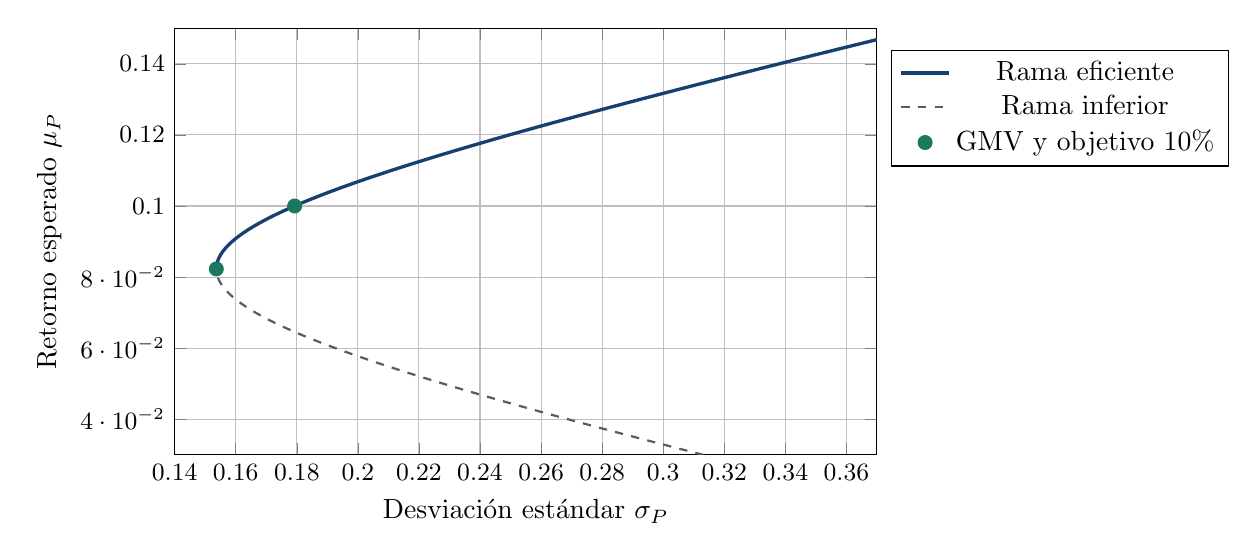
\begin{tikzpicture}
\begin{axis}[width=10.5cm,height=7cm,xlabel={Desviación estándar $\sigma_P$},ylabel={Retorno esperado $\mu_P$},grid=major,xmin=.14,xmax=.37,ymin=.03,ymax=.15,legend style={at={(1.02,.95)},anchor=north west},scaled ticks=false,tick label style={font=\small}]
\addplot[azul,very thick,domain=.08229508:.15,samples=120]({sqrt(36/1525+(1525/56)*(x-251/3050)^2)},{x});\addlegendentry{Rama eficiente}
\addplot[gris,dashed,thick,domain=.03:.08229508,samples=100]({sqrt(36/1525+(1525/56)*(x-251/3050)^2)},{x});\addlegendentry{Rama inferior}
\addplot[only marks,verde,mark=*,mark size=2.5pt]coordinates{(.15364426,.08229508)(.17928429,.10)};\addlegendentry{GMV y objetivo $10\%$}
\end{axis}\end{tikzpicture}
\caption{Frontera del ejemplo de tres activos con pesos reales y sin restricciones adicionales. La parte superior ofrece mayor retorno para cada nivel de riesgo de la frontera.}
\end{figure}
\subsection{Restricciones de no negatividad y caso singular}
Si $w_j\ge0$, las condiciones KKT para el objetivo $w\T\Sigma w/2$ son
\[
\Sigma w-\eta\ones_p-\gamma\mu-\nu=0,\quad
w\ge0,\quad\nu\ge0,\quad\nu_jw_j=0,
\]
además de las igualdades. La frontera pasa a estar formada por tramos con distintos conjuntos de activos con peso positivo. Si $\Sigma$ es singular, la inversa anterior no existe; usar pseudoinversa sin estudiar factibilidad y direcciones nulas puede omitir soluciones o riesgos nulos. Una regularización positiva permite un problema bien condicionado, pero cambia el modelo de riesgo.

\section{Factores principales de riesgo y portafolios propios}
Escribe $\Sigma=V\Lambda V\T$ y define $f=V\T(R-\mu)\in\R^{p\times1}$, con $\Cov(f)=\Lambda$. Para un portafolio $w\in\R^{p\times1}$, sus exposiciones a esos factores son $b=V\T w\in\R^{p\times1}$. Entonces
\[
R_P-\mu_P=w\T(R-\mu)=b\T f,\qquad
\boxed{\sigma_P^2=\sum_{j=1}^p\lambda_jb_j^2}.
\]
Cada término es no negativo y mide la contribución de un modo ortogonal de riesgo. Un autovector $v_j$ puede interpretarse como una combinación de activos cuya varianza, bajo norma euclidiana uno, es $\lambda_j$.
\subsection{Caso de correlación equicorrelacionada}
Supón que todos los activos tienen desviación $\sigma$ y correlación común $\rho$:
\[
\Sigma=\sigma^2[(1-\rho)I_p+\rho\ones_p\ones_p\T],\qquad -\frac1{p-1}\le\rho\le1.
\]
Para $v_1=\ones_p/\sqrt p\in\R^{p\times1}$,
\[
\Sigma v_1=\sigma^2[1+(p-1)\rho]v_1.
\]
Para cualquier $v\perp\ones_p$, $\Sigma v=\sigma^2(1-\rho)v$. Si $\rho>0$, el modo común es el dominante y los otros $p-1$ modos son contrastes. Con $w=\ones_p/p$,
\[
\sigma_P^2=\sigma^2\left[\rho+\frac{1-\rho}{p}\right].
\]
Al crecer $p$, el término específico se diluye, pero el común tiende a $\sigma^2\rho$ si $\rho>0$. Esta identidad muestra por qué diversificar muchos activos correlacionados no elimina todo el riesgo.
\subsection{Invertir la covarianza amplifica los modos pequeños}
\[
\Sigma^{-1}=\sum_j\frac1{\lambda_j}v_jv_j\T,\qquad
w_{\mathrm{GMV}}=\frac{\sum_j\lambda_j^{-1}v_j(v_j\T\ones_p)}{\sum_j\lambda_j^{-1}(v_j\T\ones_p)^2}.
\]
Autovalores pequeños reciben pesos recíprocos grandes. Un error pequeño de estimación puede cambiar mucho los pesos. Por eso un excelente ajuste de covarianza dentro de muestra no asegura una cartera estable fuera de muestra.
\subsection{Modelo de factores y riesgo residual}
Retener únicamente $\Sigma_k=V_k\Lambda_kV_k\T$ produce una matriz singular para $k<p$ y asigna riesgo cero a las direcciones descartadas. Un optimizador podría explotar esos ceros artificiales. Una opción de modelado es
\[
\widetilde\Sigma=V_k\Lambda_kV_k\T+\tau(I_p-V_kV_k\T),\quad \tau>0,
\]
que reemplaza los autovalores descartados por $\tau$. Otra es un modelo $BFB\T+D$ con $B\in\R^{p\times k}$, $F\succ0$ de dimensión $k\times k$ y $D\succ0$ diagonal de dimensión $p\times p$. Es preciso especificar cómo se estima cada parte; no es una identidad automática de PCA.

\section{Sharpe, Rayleigh generalizado y blanqueamiento del riesgo}
Sea $m=\mu-r_f\ones_p\in\R^{p\times1}$ el vector de retornos esperados en exceso de una tasa $r_f$, y supón $\Sigma\succ0$, $m\ne0$. El cociente homogéneo
\[
\mathcal Q(w)=\frac{(m\T w)^2}{w\T\Sigma w},\qquad w\ne0,
\]
es el cuadrado del cociente retorno en exceso/desviación. Definiendo $a=\Sigma^{1/2}w$ y $b=\Sigma^{-1/2}m$, ambos en $\R^{p\times1}$,
\[
(m\T w)^2=(b\T a)^2\le\norm b_2^2\norm a_2^2
=(m\T\Sigma^{-1}m)(w\T\Sigma w).
\]
Por tanto, $\mathcal Q(w)\le m\T\Sigma^{-1}m$, con igualdad cuando $w\propto\Sigma^{-1}m$. Para el cociente con signo positivo se elige la orientación con $m\T w>0$.
\subsection{La ecuación propia generalizada}
Maximizar $w\T(mm\T)w$ bajo $w\T\Sigma w=1$ produce
\[
\boxed{(mm\T)w=\rho\Sigma w},\qquad \rho=m\T\Sigma^{-1}m\text{ en el máximo}.
\]
$mm\T\in\R^{p\times p}$ tiene rango uno. Al blanquear $u=\Sigma^{1/2}w\in\R^{p\times1}$ se obtiene un problema propio ordinario para
\[
\Sigma^{-1/2}mm\T\Sigma^{-1/2}=bb\T.
\]
Si $\ones_p\T\Sigma^{-1}m\ne0$, se puede imponer presupuesto con
\[
w_T=\frac{\Sigma^{-1}m}{\ones_p\T\Sigma^{-1}m}.
\]
La orientación del retorno en exceso, las restricciones de cortos y la existencia de una tasa libre de riesgo importan para su interpretación como cartera tangente; el cociente al cuadrado por sí solo no distingue un retorno positivo de uno negativo.
\begin{idea}[La conexión completa solicitada]
PCA maximiza $v\T\Sigma v$ bajo $v\T v=1$ y da $\Sigma v=\lambda v$. Markowitz minimiza $w\T\Sigma w$ bajo presupuesto y retorno, dando $\Sigma w=\eta\ones_p+\gamma\mu$. Sharpe al cuadrado conduce a $(mm\T)w=\rho\Sigma w$. Los tres problemas comparten formas cuadráticas, proyecciones y teoría espectral, pero sus restricciones y objetivos no son iguales.
\end{idea}

\parte{XIII. Extensiones: otras geometrías y otras nociones de información}
\section{PCA ponderado y autovalores generalizados}
\subsection{Ponderar observaciones}
Sean pesos $\pi_i>0$ con $\sum_i\pi_i=1$ y $\Omega=\diag(\pi_1,\ldots,\pi_n)\in\R^{n\times n}$. Define
\[
\mu_\pi=\sum_i\pi_i x_i\in\R^{p\times1},\quad
X_\pi=X-\ones_n\mu_\pi\T\in\R^{n\times p},\quad
S_\pi=X_\pi\T\Omega X_\pi\in\R^{p\times p}.
\]
Entonces $v\T S_\pi v=\sum_i\pi_i[v\T(x_i-\mu_\pi)]^2$. PCA de esta distribución empírica ponderada se calcula haciendo SVD de $\Omega^{1/2}X_\pi$. Su normalización es probabilística; una corrección de insesgamiento adicional depende de qué representen los pesos y no se asume automáticamente.
\subsection{Ponderar variables mediante una métrica}
Sea $M\succ0$, $M\in\R^{p\times p}$, y usemos la distancia $\norm{x-y}_M^2=(x-y)\T M(x-y)$. Transformar $y_i=M^{1/2}(x_i-\bar x)\in\R^{p\times1}$ convierte esa distancia en euclidiana. La covarianza transformada es
\[
S_y=M^{1/2}SM^{1/2}\in\R^{p\times p}.
\]
Si $a_j$ es autovector unitario de $S_y$, la dirección de reconstrucción original es $b_j=M^{-1/2}a_j\in\R^{p\times1}$, con $b_i\T Mb_j=\delta_{ij}$. Para $B_k=[b_1\ \cdots\ b_k]$,
\[
z_i=B_k\T M(x_i-\bar x),\quad
\widehat x_i=\bar x+B_kB_k\T M(x_i-\bar x).
\]
El proyector $P_M=B_kB_k\T M$ puede no ser simétrico en Euclides, pero cumple $P_M^2=P_M$ y $P_M\T M=MP_M$: es ortogonal respecto a la métrica $M$.
\subsection{Teorema para una restricción cuadrática general}
Si $A=A\T$ y $B\succ0$, ambos de dimensión $p\times p$,
\[
\max_{v\T Bv=1}v\T Av\quad\Longrightarrow\quad Av=\lambda Bv.
\]
Con $u=B^{1/2}v\in\R^{p\times1}$,
\[
v\T Av=u\T(B^{-1/2}AB^{-1/2})u,\qquad u\T u=1.
\]
La matriz interior es simétrica. Por el teorema espectral tiene autovalores reales y una base ortonormal $\{u_j\}$. Al volver, $v_j=B^{-1/2}u_j$ satisface $v_i\T Bv_j=\delta_{ij}$. Esta es la razón matemática de la ortogonalidad \emph{generalizada}.

\section{Discriminante lineal y correlación canónica: ejes con otro objetivo}
\subsection{LDA: separar clases en lugar de explicar variación total}
Sean dos clases con medias $\mu_1,\mu_2\in\R^{p\times1}$ y una matriz de dispersión interna $S_W\succ0$. Define $d=\mu_1-\mu_2\in\R^{p\times1}$. Fisher propone maximizar
\[
J(v)=\frac{[v\T(\mu_1-\mu_2)]^2}{v\T S_Wv}
=\frac{v\T dd\T v}{v\T S_Wv},\qquad v\ne0.
\]
Al blanquear $u=S_W^{1/2}v$ y aplicar Cauchy--Schwarz, el máximo es $d\T S_W^{-1}d$, alcanzado cuando $v\propto S_W^{-1}d$. La condición es $dd\T v=\lambda S_Wv$. LDA usa etiquetas y busca separación relativa a dispersión interna; PCA no usa etiquetas.
\begin{ejemplo}[PCA y LDA pueden elegir ejes perpendiculares]
Supón que ambas clases tienen covarianza interna $\diag(100,1)$, pero medias $(0,2)\T$ y $(0,-2)\T$. Con clases equiprobables, la covarianza total es $\diag(100,5)$. PCA elige el eje horizontal, porque $100>5$. LDA elige el vertical, ya que $d=(0,4)\T$ y $S_W^{-1}d=(0,4)\T$ si se usa esa covarianza interna. La separación de clases ocurre donde PCA ve menos varianza.
\end{ejemplo}
\begin{figure}[H]\centering
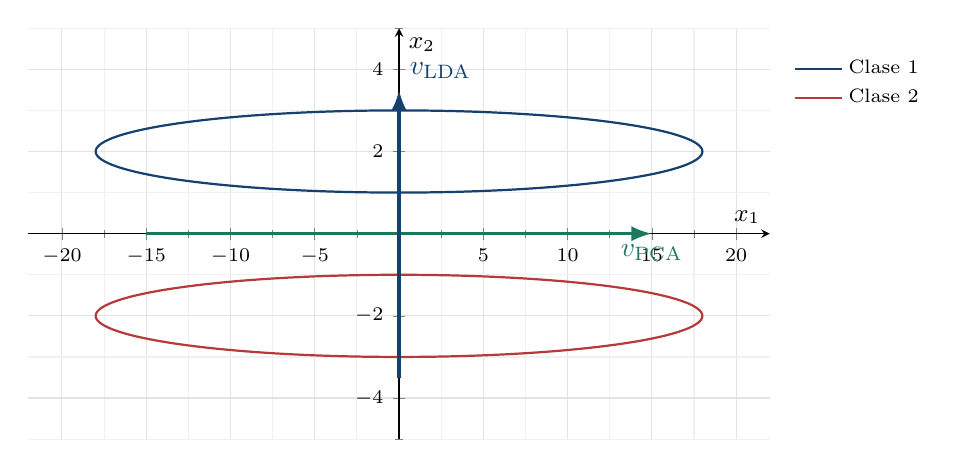
\begin{tikzpicture}
\begin{axis}[base,width=11cm,height=6.8cm,xmin=-22,xmax=22,ymin=-5,ymax=5,xlabel={$x_1$},ylabel={$x_2$},legend style={at={(1.02,.95)},anchor=north west}]
\addplot[azul,thick,domain=0:360]({18*cos(x)},{2+sin(x)});\addlegendentry{Clase 1}
\addplot[rojo,thick,domain=0:360]({18*cos(x)},{-2+sin(x)});\addlegendentry{Clase 2}
\draw[vecverde](axis cs:-15,0)--(axis cs:15,0)node[below]{$v_{\mathrm{PCA}}$};
\draw[vec](axis cs:0,-3.5)--(axis cs:0,3.5)node[above right]{$v_{\mathrm{LDA}}$};
\end{axis}\end{tikzpicture}
\caption{Esquema de clases alargadas horizontalmente pero separadas verticalmente. Las elipses ilustran la geometría; no representan una muestra ni un nivel probabilístico concreto.}
\end{figure}
\subsection{CCA: maximizar relación entre dos bloques}
Sean $x\in\R^{p\times1}$ y $y\in\R^{q\times1}$ aleatorios centrados, con covarianzas $\Sigma_{xx}\succ0$, $\Sigma_{yy}\succ0$ y cruzada $\Sigma_{xy}\in\R^{p\times q}$. CCA busca $a\in\R^{p\times1}$ y $b\in\R^{q\times1}$ que maximicen
\[
a\T\Sigma_{xy}b\quad\text{sujeto a }a\T\Sigma_{xx}a=1,\quad b\T\Sigma_{yy}b=1.
\]
Con $u=\Sigma_{xx}^{1/2}a$ y $v=\Sigma_{yy}^{1/2}b$, el problema es $\max_{\norm u=\norm v=1}u\T Kv$, donde
\[
K=\Sigma_{xx}^{-1/2}\Sigma_{xy}\Sigma_{yy}^{-1/2}\in\R^{p\times q}.
\]
La SVD $K=UDV\T$ muestra que el máximo es su mayor valor singular, $\rho_1$, y los pares siguientes usan sus restantes vectores singulares. Eliminando $b$ de las condiciones $\Sigma_{xy}b=\rho\Sigma_{xx}a$ y $\Sigma_{yx}a=\rho\Sigma_{yy}b$,
\[
\Sigma_{xy}\Sigma_{yy}^{-1}\Sigma_{yx}a=\rho^2\Sigma_{xx}a.
\]
Otra vez aparece una ecuación propia generalizada, pero aquí los autovalores son correlaciones canónicas al cuadrado.

\section{Kernel PCA: no lineal en los datos, lineal en características}
Sea $\phi:\R^p\to\mathcal H$ un mapa a un espacio de Hilbert con producto interno $\ip{\cdot}{\cdot}_{\mathcal H}$. Un núcleo válido satisface
\[
\kappa(x,y)=\ip{\phi(x)}{\phi(y)}_{\mathcal H},\qquad
K_{i\ell}=\kappa(x_i,x_\ell),\quad K\in\R^{n\times n},\quad K\succeq0.
\]
Se puede calcular PCA en $\mathcal H$ usando solo productos internos; no hace falta escribir cada coordenada de $\phi$. Este es el principio de kernel PCA.
\subsection{Centrar en el espacio correcto}
Define $\bar\phi=n^{-1}\sum_i\phi(x_i)$ y $\phi_c(x_i)=\phi(x_i)-\bar\phi$. La matriz de Gram centrada es
\[
\boxed{K_c=HKH},\qquad H=I_n-\frac1n\ones_n\ones_n\T,
\]
\[
(K_c)_{i\ell}=K_{i\ell}-\frac1n\sum_aK_{ia}-\frac1n\sum_aK_{a\ell}+\frac1{n^2}\sum_{a,b}K_{ab}.
\]
Centrar los datos $x_i$ no centra necesariamente $\phi(x_i)$ si $\phi$ es no lineal.
\subsection{Del operador de covarianza a la matriz de Gram}
Usamos el denominador $n$ en esta sección. El operador empírico es
\[
C_{\mathcal H}h=\frac1n\sum_i\phi_c(x_i)\ip{\phi_c(x_i)}h_{\mathcal H},\qquad h\in\mathcal H.
\]
Cualquier autovector $u\in\mathcal H$ de autovalor $\lambda>0$ pertenece al span de los $\phi_c(x_i)$ porque $u=\lambda^{-1}C_{\mathcal H}u$. Si $K_cq_j=\eta_jq_j$, $q_j\in\R^{n\times1}$ unitario y $\eta_j>0$, define
\[
u_j=\frac1{\sqrt{\eta_j}}\sum_i(q_j)_i\phi_c(x_i)\in\mathcal H.
\]
Entonces
\[
\norm{u_j}_{\mathcal H}^2=\frac{q_j\T K_cq_j}{\eta_j}=1,\qquad
C_{\mathcal H}u_j=\frac{\eta_j}{n}u_j.
\]
La puntuación de la observación $i$ es
\[
z_{ij}=\ip{\phi_c(x_i)}{u_j}_{\mathcal H}
=\frac{(K_cq_j)_i}{\sqrt{\eta_j}}=\sqrt{\eta_j}(q_j)_i.
\]
Así, autovalor de Gram $\eta_j$, varianza empírica $\eta_j/n$ y normalización del eje $1/\sqrt{\eta_j}$ son tres cantidades relacionadas, pero diferentes.
\subsection{Transformar un punto nuevo}
Para $x\in\R^{p\times1}$, define $k_c(x)\in\R^{n\times1}$ con entradas
\[
[k_c(x)]_i=\kappa(x_i,x)-\frac1n\sum_a\kappa(x_a,x)
-\frac1n\sum_aK_{ia}+\frac1{n^2}\sum_{a,b}K_{ab}.
\]
Entonces $z_j(x)=q_j\T k_c(x)/\sqrt{\eta_j}$. Todas las medias se refieren al conjunto de entrenamiento. Volver de una proyección en $\mathcal H$ a un punto original es el problema de preimagen; puede no tener solución exacta ni única.
\begin{ejemplo}[Núcleo cuadrático con mapa explícito]
Para $x=(x_1,x_2)\T\in\R^{2\times1}$,
\[
\phi(x)=(x_1^2,\sqrt2x_1x_2,x_2^2)\T\in\R^{3\times1},\quad
\phi(x)\T\phi(y)=x_1^2y_1^2+2x_1x_2y_1y_2+x_2^2y_2^2=(x\T y)^2.
\]
Una relación no lineal como $x_1^2+x_2^2=r^2$ se vuelve una relación lineal entre la primera y tercera características. Esto demuestra la posibilidad de linealizar estructura; no garantiza que la primera componente de cualquier núcleo separe automáticamente grupos concéntricos.
\end{ejemplo}
\subsection{Cálculo exacto con cuatro puntos}
Sean $x_1=(1,0)\T$, $x_2=(-1,0)\T$, $x_3=(0,1)\T$, $x_4=(0,-1)\T$. Para $\kappa(x,y)=(x\T y)^2$,
\[
K=\begin{pmatrix}1&1&0&0\\1&1&0&0\\0&0&1&1\\0&0&1&1\end{pmatrix},\quad
K_c=\frac12\begin{pmatrix}1&1&-1&-1\\1&1&-1&-1\\-1&-1&1&1\\-1&-1&1&1\end{pmatrix}.
\]
Hay un único autovalor positivo $\eta_1=2$, con $q_1=(1,1,-1,-1)\T/2$. Las puntuaciones son
\[
z_1=\sqrt2q_1=(1,1,-1,-1)\T/\sqrt2\in\R^{4\times1},\quad
\lambda_1(C_{\mathcal H})=\frac24=\frac12.
\]
El eje en características es $u_1=(1,0,-1)\T/\sqrt2$, por lo que $z(x)=(x_1^2-x_2^2)/\sqrt2$. Los puntos opuestos tienen la misma representación: el núcleo cuadrático no distingue $x$ de $-x$.

\section{MDS clásico: recuperar PCA a partir de distancias}
Supongamos que solo se conocen distancias euclidianas entre observaciones: $\delta_{ij}=\norm{x_i-x_j}_2$. Sea $D^{(2)}=(\delta_{ij}^2)\in\R^{n\times n}$. El escalamiento multidimensional clásico construye
\[
\boxed{B=-\frac12HD^{(2)}H\in\R^{n\times n}}.
\]
\begin{deduccion}
Sea $G=XX\T$ y $g=(G_{11},\ldots,G_{nn})\T\in\R^{n\times1}$. La identidad
\[
\delta_{ij}^2=\norm{x_i}_2^2+\norm{x_j}_2^2-2x_i\T x_j
\]
da $D^{(2)}=g\ones_n\T+\ones_ng\T-2G$. Como $H\ones_n=0$,
\[
-\frac12HD^{(2)}H=HGH=HXX\T H=X_cX_c\T.
\]
Si $X_c=U_rD_rV_r\T$, entonces $B=U_rD_r^2U_r\T$. Sus coordenadas de MDS son $Y_k=U_kD_k=X_cV_k$, exactamente las puntuaciones PCA, salvo rotaciones dentro de empates y signos.
\end{deduccion}
\subsection{Qué se puede recuperar y qué no}
Las distancias no determinan la traslación, rotación o reflexión del sistema original; sí determinan su geometría euclidiana hasta esas transformaciones cuando hay información suficiente. Si las disimilitudes no son euclidianas, $B$ puede tener autovalores negativos. Descartarlos aproxima otra geometría, pero ya no reproduce exactamente esas disimilitudes.
\subsection{Isomap y la diferencia entre distancia recta y distancia sobre una superficie}
Isomap sustituye distancias euclidianas por distancias de caminos mínimos en un grafo de vecinos y después aplica MDS. Busca aproximar distancias geodésicas de una variedad. Su resultado depende de que el grafo capture bien vecindades; atajos entre pliegues o componentes desconectados pueden alterar fuertemente la representación. Esta sección presenta el principio, no una garantía general de recuperación de variedades.

\section{Proyecciones aleatorias y conservación probabilística de distancias}
PCA elige ejes a partir de la covarianza. Una proyección aleatoria puede preservar aproximadamente todas las distancias de un conjunto finito sin estimar esos ejes. Sea $R\in\R^{k\times p}$ con entradas independientes $N(0,1/k)$ y define $f(x)=Rx\in\R^{k\times1}$.
\subsection{Una dirección fija y una variable chi-cuadrado}
Para $d\in\R^{p\times1}\setminus\{0\}$ fijo, cada entrada de $Rd$ es $N(0,\norm d_2^2/k)$ y son independientes. Por tanto,
\[
\frac{\norm{Rd}_2^2}{\norm d_2^2}\ \overset{d}=\ \frac{Y}{k},\qquad Y\sim\chi_k^2.
\]
En particular, $\E\norm{Rd}_2^2=\norm d_2^2$. Preservar en esperanza no basta; necesitamos concentración.
\subsection{Cota de concentración: derivación por Chernoff}
La función generadora de momentos es $\E e^{tY}=(1-2t)^{-k/2}$ para $t<1/2$. Para $0<\varepsilon<1$ y $t>0$,
\[
\Pr\{Y\ge k(1+\varepsilon)\}\le e^{-tk(1+\varepsilon)}(1-2t)^{-k/2}.
\]
Se minimiza con $t=\varepsilon/[2(1+\varepsilon)]$, dando
\[
\Pr\{Y\ge k(1+\varepsilon)\}\le
\exp\left[-\frac k2(\varepsilon-\log(1+\varepsilon))\right]
\le\exp\left[-k\left(\frac{\varepsilon^2}4-\frac{\varepsilon^3}6\right)\right].
\]
La última cota usa $\log(1+\varepsilon)\le\varepsilon-\varepsilon^2/2+\varepsilon^3/3$. El mismo argumento con $t<0$ produce una cota inferior al menos tan fuerte para la cola baja. Combinándolas,
\[
\Pr\left\{\left|\frac{\norm{Rd}_2^2}{\norm d_2^2}-1\right|>\varepsilon\right\}
\le2\exp\left[-k\left(\frac{\varepsilon^2}4-\frac{\varepsilon^3}6\right)\right].
\]
\subsection{De un par a todos los pares: lema de Johnson--Lindenstrauss}
Para $N$ puntos hay $M=N(N-1)/2$ pares. Por la cota de la unión, si
\[
k\ge\frac{\log(2M/\delta)}{\varepsilon^2/4-\varepsilon^3/6},\qquad0<\delta<1,
\]
con probabilidad al menos $1-\delta$ todas sus distancias cuadradas cumplen
\[
(1-\varepsilon)\norm{x_i-x_j}_2^2\le\norm{Rx_i-Rx_j}_2^2
\le(1+\varepsilon)\norm{x_i-x_j}_2^2.
\]
La dependencia es del orden $\varepsilon^{-2}\log(N/\delta)$, no lineal en $p$. La cota suficiente puede ser conservadora e incluso dar $k\ge p$ para tolerancias estrictas; no promete compresión útil en todo problema.
\begin{cuidado}[Objetivos diferentes]
PCA es óptimo para reconstrucción cuadrática mediante proyección ortogonal de rango fijo. Una proyección gaussiana reescalada no es generalmente ortogonal ni minimiza ese error, pero ofrece una garantía probabilística uniforme sobre distancias de un conjunto finito. Ninguno de estos enunciados domina al otro en todos los usos.
\end{cuidado}

\section{Grafos, Laplacianos y mapas no lineales}
\subsection{Otra ecuación espectral: conservar vecindades}
Sea $W=(w_{ij})\in\R^{n\times n}$ una matriz simétrica de pesos no negativos de un grafo, $D=\diag(d_1,\ldots,d_n)$ con $d_i=\sum_jw_{ij}$, y $L=D-W$. Para $y=(y_1,\ldots,y_n)\T\in\R^{n\times1}$,
\[
\boxed{y\T Ly=\frac12\sum_{i,j}w_{ij}(y_i-y_j)^2\ge0}.
\]
\textbf{Demostración.} Expandir los cuadrados da $\frac12\sum_{ij}w_{ij}(y_i^2+y_j^2-2y_iy_j)=\sum_i d_i y_i^2-\sum_{ij}w_{ij}y_iy_j$. Por simetría esto coincide con $y\T(D-W)y$.

Suponiendo $d_i>0$ (sin nodos aislados), minimizar esta energía con $y\T Dy=1$ y $y\T D\ones_n=0$ conduce a $Ly=\lambda Dy$. Se usan autovalores pequeños no triviales para ubicar cerca los nodos fuertemente conectados. En PCA se retienen autovalores \emph{grandes} de una covarianza; aquí pequeños de un Laplaciano: el significado del operador importa.
\subsection{Una cadena de tres nodos}
Para pesos unitarios entre 1--2 y 2--3,
\[
L=\begin{pmatrix}1&-1&0\\-1&2&-1\\0&-1&1\end{pmatrix},\quad
L(1,1,1)\T=0,\quad L(1,0,-1)\T=(1,0,-1)\T,
\]
\[
L(1,-2,1)\T=3(1,-2,1)\T.
\]
En la versión no normalizada con $y\T y=1$, el primer autovector no constante ordena los nodos como $1,0,-1$: representa la cadena en una recta. El autovalor cero corresponde a la coordenada constante y no aporta separación.
\subsection{t-SNE y UMAP: alcance de la comparación}
\textbf{t-SNE} transforma cercanías entre observaciones en probabilidades $p_{ij}$ y ajusta coordenadas $y_i\in\R^{k\times1}$ con afinidades $q_{ij}$ basadas en una distribución de colas pesadas. Minimiza $\sum_{i\ne j}p_{ij}\log(p_{ij}/q_{ij})$. Es una optimización no convexa de vecindades; sus ejes no son componentes principales y no tienen porcentajes de varianza explicada. El artículo original de van der Maaten y Hinton está en las referencias.

\textbf{UMAP} construye una representación ponderada de vecindades y optimiza una disposición en menor dimensión a partir de ella. Su planteamiento y parámetros difieren de t-SNE; tampoco se obtiene por diagonalizar la covarianza. Se remite al trabajo de McInnes, Healy y Melville para su construcción completa. En ambos casos, distancias entre grupos, tamaños visuales y huecos pueden depender fuertemente de parámetros y optimización; una figura separada no sustituye una comprobación estadística de grupos.
\begin{center}\small
\begin{tabular}{>{\raggedright\arraybackslash}p{2.8cm}>{\raggedright\arraybackslash}p{4.0cm}>{\raggedright\arraybackslash}p{3.5cm}>{\raggedright\arraybackslash}p{4.6cm}}\toprule
Método & Objeto principal & Estructura & Significado del eje\\\midrule
PCA & Covarianza & Lineal & Combinación de variables\\
Kernel PCA & Gram de características & No lineal en $x$ & Eje en un espacio de Hilbert\\
MDS clásico & Distancias al cuadrado & Euclidiana si es posible & Coordenada geométrica\\
Proyección aleatoria & Mapa aleatorio & Lineal & Dirección aleatoria reescalada\\
Laplaciano & Grafo de vecinos & Local & Función suave sobre nodos\\
t-SNE / UMAP & Afinidades de vecinos & No lineal & Coordenada del mapa ajustado\\\bottomrule
\end{tabular}\end{center}

\section{PCA en espacios de funciones: conexión directa con L2}
Sea $\mathcal H=L^2([0,1])$ con $\ip fg=\int_0^1f(t)g(t)\dd t$. Ahora una observación es una curva aleatoria $X\in\mathcal H$ y suponemos $\E\norm X_{\mathcal H}^2<\infty$. Su media es $m(t)=\E[X(t)]$ en el sentido apropiado de $L^2$. Definimos el operador de covarianza
\[
Cf=\E[\ip{X-m}f_{\mathcal H}(X-m)],\qquad f\in\mathcal H.
\]
Cuando se representa mediante un núcleo de covarianza,
\[
(Cf)(s)=\int_0^1K(s,t)f(t)\dd t,\qquad
K(s,t)=\Cov(X(s),X(t)).
\]
La integral hace el papel de la suma matricial. La ecuación propia es
\[
\boxed{\int_0^1K(s,t)\phi_j(t)\dd t=\lambda_j\phi_j(s)},\qquad
\int_0^1\phi_i(t)\phi_j(t)\dd t=\delta_{ij}.
\]
\subsection{Propiedades del operador}
\[
\ip{Cf}g=\E[\ip{X-m}f\ip{X-m}g]=\ip f{Cg},\qquad
\ip{Cf}f=\E[\ip{X-m}f^2]\ge0.
\]
Así, $C$ es autoadjunto y positivo. Bajo el segundo momento finito en un Hilbert separable, es de traza finita y compacto, con $\tr C=\E\norm{X-m}_{\mathcal H}^2$. El teorema espectral para operadores compactos positivos proporciona autovalores no negativos y funciones propias ortonormales en el soporte de la covarianza. La demostración completa de ese teorema funcional requiere análisis de operadores; aquí se explicitan sus consecuencias y la optimalidad de la truncación.
\subsection{Expansión de Karhunen--Loève y error de truncación}
Define puntuaciones aleatorias $\xi_j=\ip{X-m}{\phi_j}_{\mathcal H}\in\R$. Entonces
\[
\E[\xi_j]=0,\quad\E[\xi_i\xi_j]=\lambda_j\delta_{ij},\quad
X=m+\sum_{j\ge1}\xi_j\phi_j\quad\text{en }L^2(\Omega;\mathcal H),
\]
\[
\widehat X_k=m+\sum_{j=1}^k\xi_j\phi_j,\qquad
\boxed{\E\norm{X-\widehat X_k}_{\mathcal H}^2=\sum_{j>k}\lambda_j}.
\]
\textbf{Deducción del error.} Por ortogonalidad, la norma cuadrada del residuo es la suma de cuadrados de las coordenadas descartadas; tomar esperanza y usar Tonelli da $\sum_{j>k}\E\xi_j^2=\sum_{j>k}\lambda_j$. Para cualquier familia ortonormal $g_1,\ldots,g_k$, la varianza capturada es $\sum_\ell\ip{Cg_\ell}{g_\ell}$ y el mismo argumento de máxima traza da una cota $\sum_{j\le k}\lambda_j$. Por tanto, las funciones propias maximizan captura y minimizan error esperado.
\begin{ejemplo}[Un proceso de curvas con dos componentes exactas]
Sean $A,B$ aleatorios centrados, incorrelacionados, $\Var(A)=4$, $\Var(B)=1$. Define
\[
X(t)=A\phi_1(t)+B\phi_2(t),\quad
\phi_1(t)=1,\quad\phi_2(t)=\sqrt{12}(t-1/2),\quad0\le t\le1.
\]
Comprobamos $\int_0^1\phi_1^2=1$, $\int_0^1\phi_2^2=12(1/12)=1$ y $\int_0^1\phi_1\phi_2=0$. El núcleo es
\[
K(s,t)=4\phi_1(s)\phi_1(t)+\phi_2(s)\phi_2(t).
\]
Por integración, $C\phi_1=4\phi_1$ y $C\phi_2=\phi_2$. Retener solo $A\phi_1$ captura $4/5=80\%$ de variación integrada y deja error esperado uno. La primera componente cambia el nivel; la segunda, la pendiente.
\end{ejemplo}
\begin{figure}[H]\centering
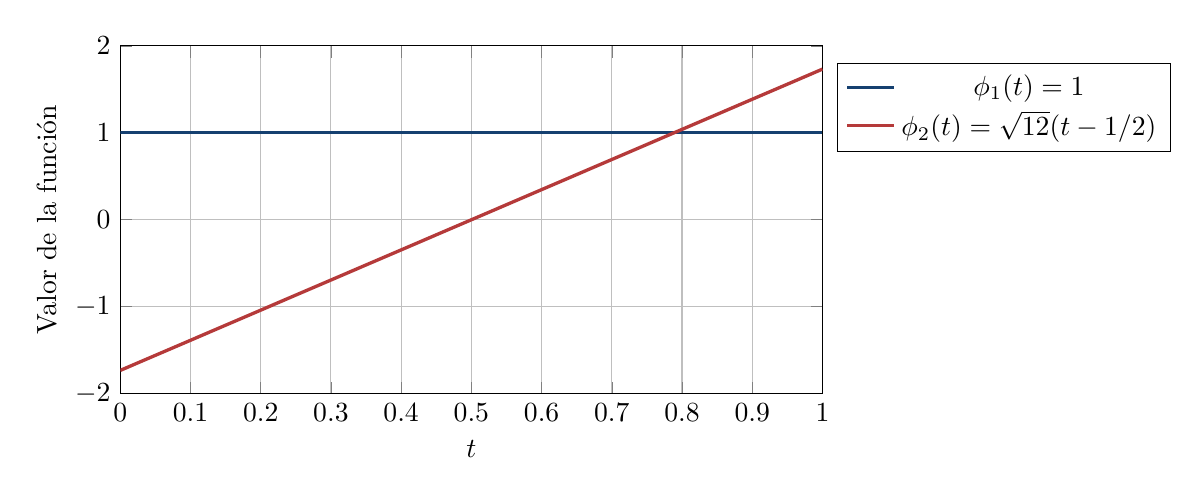
\begin{tikzpicture}
\begin{axis}[width=10.5cm,height=6cm,xlabel={$t$},ylabel={Valor de la función},xmin=0,xmax=1,ymin=-2,ymax=2,grid=major,legend style={at={(1.02,.95)},anchor=north west}]
\addplot[azul,very thick,domain=0:1]{1};\addlegendentry{$\phi_1(t)=1$}
\addplot[rojo,very thick,domain=0:1]{sqrt(12)*(x-.5)};\addlegendentry{$\phi_2(t)=\sqrt{12}(t-1/2)$}
\end{axis}\end{tikzpicture}
\caption{Funciones propias ortonormales en $L^2([0,1])$. El producto interno es una integral; no exige que las curvas sean perpendiculares como trazos en el papel.}
\end{figure}
\subsection{Discretizar una curva cambia la métrica si se ignoran los pesos}
Si una curva se mide en puntos $t_1,\ldots,t_p$ con pesos de cuadratura $\omega_j>0$, la integral se aproxima por $\sum_j\omega_jf(t_j)g(t_j)$. Definiendo $M=\diag(\omega_1,\ldots,\omega_p)$, se vuelve a PCA con métrica $M$. Hacer PCA ordinario sobre una malla irregular sin pesos puede dar importancia excesiva a regiones donde se midió más densamente.

\parte{XIV. Alta dimensión: riesgo matricial e incertidumbre de los ejes}
\section{Cuando la dimensión compite con el tamaño de la muestra}
Muchas fórmulas elementales se mantienen, pero cambia su escala. Para $x_i\sim\mathcal N_p(0,I_p)$ independientes,
\[
\E\norm{\bar x}_2^2=p/n.
\]
Cada coordenada tiene varianza $1/n$, mientras el error conjunto suma $p$ coordenadas. Si $p/n\to c>0$, el error en norma no tiende a cero por el mismo argumento de dimensión fija. En $p=1000,n=200$, la raíz del error cuadrático medio vectorial es $\sqrt5$, pese a que cada coordenada tiene error estándar $1/\sqrt{200}$.
\subsection{La masa gaussiana se aleja del origen}
Para $z\sim\mathcal N_p(0,I_p)$, $\norm z_2^2\sim\chi^2_p$. Chebyshev da
\[
\Prob\!\left(\left|\frac{\norm z_2^2}p-1\right|\ge\delta\right)
\le\frac2{p\delta^2}.
\]
El radio se concentra alrededor de $\sqrt p$. Dos vectores independientes $z,z'$ tienen $z-z'\sim\mathcal N_p(0,2I_p)$ y distancia cuadrada media $2p$, varianza $8p$. El coeficiente de variación de la \emph{distancia cuadrada} es $\sqrt{2/p}$. Una nube puede estar muy dispersa en radio absoluto y tener distancias relativas muy parecidas.

\begin{figure}[H]\centering
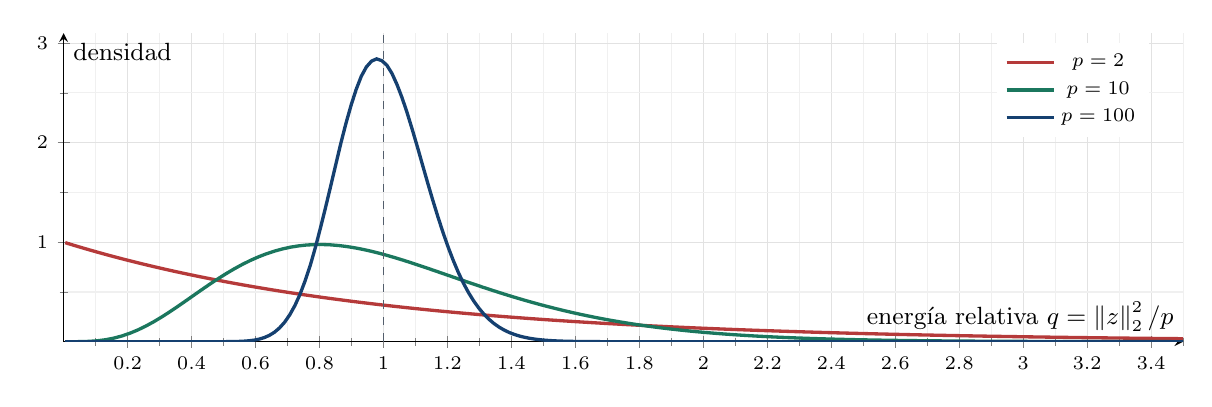
\begin{tikzpicture}\begin{axis}[base,width=15.8cm,height=5.5cm,xmin=0,xmax=3.5,ymin=0,ymax=3.1,xlabel={energía relativa $q=\norm z_2^2/p$},ylabel={densidad},legend pos=north east]
\addplot[rojo,very thick,domain=.005:3.5]{exp(-x)};\addlegendentry{$p=2$}
\addplot[verde,very thick,domain=.005:3.5]{exp(5*ln(5)-ln(24)+4*ln(x)-5*x)};\addlegendentry{$p=10$}
\addplot[azul,very thick,domain=.005:3.5,samples=220]{exp(51.03540632506241+49*ln(x)-50*x)};\addlegendentry{$p=100$}
\draw[gris,dashed](axis cs:1,0)--(axis cs:1,3.1);
\end{axis}\end{tikzpicture}
\caption{Densidad exacta de $\chi_p^2/p$: $f(q)=(p/2)^{p/2}q^{p/2-1}e^{-pq/2}/\Gamma(p/2)$. Su media es uno y su varianza $2/p$; aumentar dimensión concentra la energía relativa.}
\end{figure}

\subsection{Ángulos casi rectos, con una prueba por simetría}
Las direcciones $u=z/\norm z_2$ y $v=z'/\norm z'_2$ son independientes y uniformes sobre la esfera. Por simetría $\E(vv\T)=I_p/p$: las diagonales son iguales y suman uno, y las entradas fuera de diagonal se anulan al cambiar signos. Condicionado a $u$,
\[
\E[(u\T v)^2\mid u]=u\T\E(vv\T)u=1/p.
\]
Así $\Prob(|u\T v|>\delta)\le1/(p\delta^2)$. No significa que cualquier conjunto de vectores sea ortogonal; se refiere a este modelo aleatorio independiente.

\section{Riesgo exacto de una covarianza y regularización por contracción}
Con muestra gaussiana y $S$ insesgada, sumar las varianzas de todas sus entradas produce
\begin{align*}
\E\norm{S-\Sigma}\F^2
&=\sum_{i,j}\Var(S_{ij})\\
&=\frac1{n-1}\sum_{i,j}(\Sigma_{ii}\Sigma_{jj}+\Sigma_{ij}^2)\\
&=\boxed{\frac{(\tr\Sigma)^2+\norm\Sigma\F^2}{n-1}}.
\end{align*}
Para $\Sigma=I_p$, el error es $p(p+1)/(n-1)$ y su cociente con $\norm\Sigma\F^2=p$ es $(p+1)/(n-1)$. En $p=1000,n=200$ ese error relativo cuadrático esperado es $1001/199\approx5.030$. Insesgamiento entrada por entrada no garantiza una matriz global precisa.
\subsection{Una contracción con riesgo calculable}
Para un objetivo determinista $T=\tau I_p$, $\tau>0$, considera $S_\eta=\eta S+(1-\eta)T$, $0\le\eta\le1$. Entonces
\[
\E S_\eta-\Sigma=(1-\eta)(T-\Sigma),
\]
\[
\E\norm{S_\eta-\Sigma}\F^2=\eta^2 V+(1-\eta)^2B^2,
\quad V=\E\norm{S-\Sigma}\F^2,\quad B^2=\norm{T-\Sigma}\F^2.
\]
El término cruzado desaparece porque $\E(S-\Sigma)=0$. Derivar esta cuadrática da $\eta_*=B^2/(V+B^2)$ si el denominador es positivo. Es un valor \emph{oráculo}: depende de la covarianza desconocida. Si $\tau$ se estima de la muestra, deja de ser un objetivo determinista y hay que incluir su covarianza con $S$ en el cálculo del riesgo.
Para $\eta<1$, todos los autovalores de $S_\eta$ son al menos $(1-\eta)\tau$, incluso si $S$ es singular. La regularización reduce varianza e impone una hipótesis de estructura; no genera información gratis.
\subsection{Bajo rango más diagonal: invertir miles de variables con un sistema pequeño}
Sea $\Sigma=D+BB\T$, donde $D\in\R^{p\times p}$ es diagonal positiva y $B\in\R^{p\times k}$, $k\ll p$. Multiplicar bloques o verificar el producto con $\Sigma$ prueba la identidad de Woodbury:
\[
\boxed{\Sigma^{-1}=D^{-1}-D^{-1}B(I_k+B\T D^{-1}B)^{-1}B\T D^{-1}}.
\]
La matriz invertida en el centro es $k\times k$. El lema del determinante da
\[
\det\Sigma=\det D\,\det(I_k+B\T D^{-1}B).
\]
Para comprobar la primera fórmula, escribe $M=I+B\T D^{-1}B$: al multiplicar, los términos no triviales se reducen a $B[I-M^{-1}-(M-I)M^{-1}]B\T D^{-1}=0$. La identidad del determinante sale de eliminar bloques en $\begin{psmallmatrix}D&B\\-B\T&I\end{psmallmatrix}$ en los dos órdenes posibles.
Con $p=10000,k=20$, el factor necesita $200000$ números, frente a $10^8$ de una covarianza densa. El supuesto de factores debe justificarse estadísticamente, pero su ventaja algebraica es exacta.

\section{Regresión con más coeficientes que observaciones}
Si $p>n$, $X\T X$ es singular. El problema MCO sigue siendo minimizar $\norm{y-Xb}_2^2$; el conjunto de soluciones es
\[
\widehat\beta=X^+y+h,\quad h\in\kerop X.
\]
La solución de norma mínima elige $h=0$. Si $\E(u\mid X)=0$ y $\Cov(u\mid X)=\sigma^2I_n$,
\[
\E(\widehat\beta_{\min}\mid X)=X^+X\beta=:P_{\rm fila}\beta,
\quad\Cov(\widehat\beta_{\min}\mid X)=\sigma^2X^+(X^+)\T.
\]
El sesgo es $-(I-P_{\rm fila})\beta$. $P_{\rm fila}$ proyecta sobre el espacio fila de $X$. Los coeficientes en su núcleo son no identificables a partir de la distribución de $y$ dada $X$.
\subsection{Una varianza cero puede esconder falta de identificación}
Si $h\in\kerop X$, $h\T\widehat\beta_{\min}=0$ siempre y su varianza es cero. Eso no demuestra que $h\T\beta=0$: el algoritmo fijó una convención. Los parámetros $\beta$ y $\beta+th$ generan la misma media $X\beta$ para cualquier $t$. Incertidumbre de un estimador seleccionado y falta de identificación de un parámetro no son lo mismo.
\begin{ejemplo}[Dos observaciones, tres coeficientes]
\[
X=\begin{pmatrix}1&0&1\\0&1&1\end{pmatrix},\quad
X^+=\frac13\begin{pmatrix}2&-1\\-1&2\\1&1\end{pmatrix},\quad
P_{\rm fila}=\frac13\begin{pmatrix}2&-1&1\\-1&2&1\\1&1&2\end{pmatrix}.
\]
Para $\beta=(1,1,1)\T$, la esperanza de la solución mínima es $(2/3,2/3,4/3)\T$ y su covarianza
\[
\frac{\sigma^2}{9}\begin{pmatrix}5&-4&1\\-4&5&1\\1&1&2\end{pmatrix}.
\]
El núcleo lo genera $(-1,-1,1)\T$. La misma álgebra opera con $n=200,p=10000$: no es necesario formar un sistema de $10000$ ecuaciones cuadráticas si podemos trabajar en el espacio de observaciones.
\end{ejemplo}
\subsection{Ridge restaura una solución única pero introduce sesgo}
Para $\lambda>0$,
\[
\widehat\beta_\lambda=(X\T X+\lambda I_p)^{-1}X\T y=:A_\lambda y.
\]
Con diseño fijo exógeno,
\[
\E\widehat\beta_\lambda=A_\lambda X\beta,
\quad b_\lambda=-\lambda(X\T X+\lambda I)^{-1}\beta,
\quad\Cov(\widehat\beta_\lambda)=A_\lambda\Omega_XA_\lambda\T.
\]
Si los errores son esféricos, el último término es $\sigma^2(X\T X+\lambda I)^{-1}X\T X(X\T X+\lambda I)^{-1}$. La identidad
\[
(X\T X+\lambda I_p)^{-1}X\T=X\T(XX\T+\lambda I_n)^{-1}
\]
se comprueba multiplicando por $X\T X+\lambda I_p$. Permite resolver un sistema $n\times n$ cuando $p\gg n$. El intercepto suele tratarse aparte para no penalizarlo.

\section{Incertidumbre de PCA: un eje estimado no es un eje fijo}
Sea $\Sigma v_j=\lambda_jv_j$ con autovalores distintos y $S=\Sigma+E$. Escribimos $\widehat\lambda_i=\lambda_i+\delta\lambda_i$, $\widehat v_i=v_i+\delta v_i$. A primer orden,
\[
\Sigma\delta v_i+Ev_i=\lambda_i\delta v_i+\delta\lambda_i v_i.
\]
Premultiplicar por $v_i\T$ da $\delta\lambda_i=v_i\T Ev_i$. Para $j\ne i$,
\[
v_j\T\delta v_i=\frac{v_j\T Ev_i}{\lambda_i-\lambda_j},\quad
\boxed{\delta v_i=\sum_{j\ne i}v_j\frac{v_j\T Ev_i}{\lambda_i-\lambda_j}}.
\]
La normalización impone $v_i\T\delta v_i=0$ a primer orden. Se orienta $\widehat v_i$ para que $\widehat v_i\T v_i>0$, evitando el cambio arbitrario de signo.
\subsection{Varianzas de autovalores y de coeficientes del eje}
Para datos gaussianos y $p$ fijo, la covarianza Wishart en la base propia da
\[
\Var(v_i\T Ev_i)=\frac{2\lambda_i^2}{n-1},\quad
\Cov(v_j\T Ev_i,v_k\T Ev_i)=\frac{\lambda_i\lambda_j}{n-1}\delta_{jk}\quad(j,k\ne i).
\]
Por tanto las aproximaciones de primer orden son
\[
\Var(\widehat\lambda_i)\approx\frac{2\lambda_i^2}{n-1},\quad
\Cov(\widehat v_i)\approx\frac1{n-1}\sum_{j\ne i}
\frac{\lambda_i\lambda_j}{(\lambda_i-\lambda_j)^2}v_jv_j\T.
\]
No son identidades exactas de los autovalores muestrales: estos son funciones no lineales de $S$. La aproximación necesita perturbación pequeña frente a las brechas y dimensión fija. Si dos autovalores coinciden, esos ejes individuales no están identificados; debe estudiarse el proyector del subespacio completo.
\subsection{Puntuaciones de entrenamiento frente a puntuaciones nuevas}
Si $\widehat V_k$ y $\bar x$ se estiman con la muestra, las puntuaciones de entrenamiento tienen media muestral cero y covarianza muestral diagonal por construcción. Para una observación nueva $\xi$ independiente de entrenamiento,
\[
z_{\rm nuevo}=\widehat V_k\T(\xi-\bar x),
\]
\[
\E(z_{\rm nuevo}\mid D)=\widehat V_k\T(\mu-\bar x),\quad
\Cov(z_{\rm nuevo}\mid D)=\widehat V_k\T\Sigma\widehat V_k.
\]
La covarianza nueva no tiene por qué ser diagonal: los ejes muestrales diagonalizan $S$, no exactamente $\Sigma$. Si $\xi$ es normal, esta distribución condicional sigue siendo normal, con esas media y covarianza.
\subsection{Error de reconstrucción fuera de la muestra}
Con $\widehat P=\widehat V_k\widehat V_k\T$, reconstruimos $\widehat\xi=\bar x+\widehat P(\xi-\bar x)$. Entonces
\[
\E(\norm{\xi-\widehat\xi}_2^2\mid D)
=\tr[(I-\widehat P)\Sigma]+\norm{(I-\widehat P)(\mu-\bar x)}_2^2.
\]
Se deduce de la esperanza de una forma cuadrática y de $(I-\widehat P)^2=I-\widehat P$. El primer término mide variación poblacional descartada; el segundo, error de centrar. La suma de autovalores muestrales descartados es error de entrenamiento, no automáticamente riesgo poblacional.

\section{Un laboratorio de mil variables con estructura conocida}
Sea $p=1000$, $n=200$ y $\xi=\mu+az+\varepsilon$, con $a=\ones_{1000}$, $z\sim\mathcal N(0,1)$ y $\varepsilon\sim\mathcal N_{1000}(0,I)$ independiente. Entonces
\[
\Sigma=I_{1000}+\ones_{1000}\ones_{1000}\T,
\quad v_1=\ones_{1000}/\sqrt{1000},\quad\lambda_1=1001,
\]
y las otras $999$ direcciones tienen autovalor uno. La varianza total es $2000$ y una componente explica $1001/2000=50.05\%$. El factor común domina \emph{cada correlación} de dos variables con valor $1/2$, pero no absorbe todo el ruido acumulado en $999$ direcciones.
\subsection{Puntuación y reconstrucción poblacionales}
\[
\eta_1=v_1\T(\xi-\mu)=\sqrt{1000}\,z+v_1\T\varepsilon
\sim\mathcal N(0,1001).
\]
El residuo $(I-v_1v_1\T)(\xi-\mu)$ es normal singular, independiente de $\eta_1$, con covarianza $I-v_1v_1\T$ y error cuadrático esperado $999$. La covarianza muestral tiene rango a lo sumo $199$, aunque la covarianza poblacional tenga rango $1000$.
\subsection{Inversa exacta por un solo factor}
\[
\Sigma^{-1}=I_{1000}-\frac{\ones_{1000}\ones_{1000}\T}{1001}.
\]
Para $h$ de suma cero, $h\T\Sigma^{-1}h=\norm h_2^2$. Para $h=t\ones_{1000}$, la distancia cuadrada es $1000t^2/1001$, mientras Euclides da $1000t^2$. La diferencia común es habitual bajo el factor y se estandariza fuertemente; la diferencia entre coordenadas conserva su coste.
\subsection{Qué combina este ejemplo}
El mismo modelo reúne espacio vectorial de dimensión mil, un factor latente, normal multivariada, covarianza como forma cuadrática, PCA como dirección de máxima varianza, reconstrucción como proyección y Mahalanobis como blanqueamiento. No necesitamos dibujar mil ejes para calcular cada objeto con precisión.

\parte{XV. Cálculo numérico, estabilidad y variantes de PCA}
\section{Cómo calcular PCA sin confundir álgebra con cómputo}
\subsection{Ruta algebraica y ruta numérica}
Para matrices pequeñas, resolver $\det(S-\lambda I_p)=0$ enseña el significado de autovalores. Para matrices grandes, expandir el polinomio característico es una mala estrategia numérica. Una implementación usa algoritmos de autovalores simétricos o una SVD, no fórmulas de raíces de un polinomio de alto grado.

La ruta más directa con datos es: centrar, estandarizar si corresponde, calcular SVD, ordenar valores singulares, escoger $k$, formar puntuaciones y reconstruir. La SVD entrega los valores singulares no negativos en orden descendente en las implementaciones usuales, pero una rutina general de autovalores puede usar otro orden; hay que conservar emparejadas columnas y autovalores al reordenar.
\subsection{Por qué formar la covarianza puede perder precisión}
Si $X_c$ tiene valores singulares positivos $d_1\ge\cdots\ge d_r>0$, el condicionamiento sobre su rango es
\[
\kappa_2(X_c)=d_1/d_r,\qquad
\kappa_2(X_c\T X_c\text{ sobre su rango})=d_1^2/d_r^2=\kappa_2(X_c)^2.
\]
Si $X_c$ es singular, el condicionamiento de una inversa completa es infinito. La igualdad sobre el rango explica por qué elevar al cuadrado mediante $X_c\T X_c$ puede empeorar la separación numérica de valores muy pequeños. La SVD evita formar explícitamente ese producto.
\subsection{Costes y tolerancias}
Para una matriz densa $n\times p$, una SVD completa/económica cuesta del orden $np\min(n,p)$ operaciones. Si solo interesan unas pocas componentes, métodos iterativos o aleatorizados pueden reducir el coste. Los autovalores negativos diminutos que aparecen al diagonalizar una covarianza calculada en punto flotante pueden ser redondeo; negativos grandes obligan a revisar construcción, faltantes y simetría. No se deben cambiar signos arbitrariamente para esconder un problema.
\subsection{Qué comprobaciones tienen significado matemático}
Con ejes $V_k$, puntuaciones $Z_k$ y autovalores $\lambda_j$, comprobar
\[
\norm{V_k\T V_k-I_k}\F\approx0,\qquad
\norm{SV_k-V_k\Lambda_k}\F\approx0,
\]
\[
\norm{Z_k-X_cV_k}\F\approx0,\qquad
\norm{X_c-X_cV_kV_k\T}\F^2\approx(n-1)\sum_{j>k}\lambda_j.
\]
Las tolerancias deben escalar con magnitud y precisión numérica. Comparar signos de autovectores literalmente es una mala prueba; comparar proyectores $V_kV_k\T$ es apropiado cuando solo importa el subespacio.

\section{Método de la potencia, deflación y actualización en línea}
\subsection{Método de la potencia: prueba de convergencia direccional}
Sea $S\succeq0$, $\lambda_1>\lambda_2\ge0$ y $v^{(0)}\in\R^{p\times1}$ con componente no nula sobre $v_1$. Iteramos
\[
y^{(t+1)}=Sv^{(t)},\qquad v^{(t+1)}=\frac{y^{(t+1)}}{\norm{y^{(t+1)}}_2}.
\]
Si $v^{(0)}=\sum_j a_jv_j$ y $a_1\ne0$,
\[
S^tv^{(0)}=\lambda_1^t\left[a_1v_1+\sum_{j>1}a_j\left(\frac{\lambda_j}{\lambda_1}\right)^tv_j\right].
\]
Al normalizar, los términos restantes se anulan geométricamente; el límite es $\operatorname{sign}(a_1)v_1$. La rapidez depende de $\lambda_2/\lambda_1$: una brecha pequeña produce convergencia lenta. Si $a_1=0$, el método no puede recuperar esa componente en aritmética exacta.
\begin{ejemplo}[Dos iteraciones y la dirección límite]
Para $S=\begin{psmallmatrix}3&1\\1&3\end{psmallmatrix}$ y $v^{(0)}=(1,0)\T$,
\[
v^{(1)}=\frac{(3,1)\T}{\sqrt{10}},\qquad
v^{(2)}=\frac{(10,6)\T}{\sqrt{136}}=\frac{(5,3)\T}{\sqrt{34}},\qquad
v^{(t)}\longrightarrow\frac{(1,1)\T}{\sqrt2}.
\]
Los cocientes de Rayleigh son $3$, $3.6$ y $66/17\approx3.88235$, acercándose al autovalor máximo $4$.
\end{ejemplo}
\subsection{Deflación e iteración por subespacios}
Si se conocen exactamente $v_1,\lambda_1$, define $S^{(1)}=S-\lambda_1v_1v_1\T$. Entonces $S^{(1)}v_1=0$ y $S^{(1)}v_j=\lambda_jv_j$ para $j>1$. Repetir recupera otras componentes. En punto flotante, errores de deflación se acumulan; una iteración de subespacios actualiza simultáneamente $W\leftarrow SW$ y reortogonaliza sus columnas.
\subsection{Regla de Oja: una idea de PCA en línea}
Si llega una observación centrada $x_t\in\R^{p\times1}$, una actualización aproximada sobre la esfera es
\[
y_t=v_t\T x_t,\qquad
\widetilde v_{t+1}=v_t+\eta_t y_t(x_t-y_tv_t),\qquad
v_{t+1}=\frac{\widetilde v_{t+1}}{\norm{\widetilde v_{t+1}}_2}.
\]
En esperanza, el incremento sin normalizar es proporcional a $\Sigma v_t-(v_t\T\Sigma v_t)v_t$, que es el gradiente de Rayleigh proyectado al plano tangente de la esfera. La convergencia requiere condiciones sobre datos, pasos $\eta_t$ y brecha espectral; la fórmula sola no constituye una garantía universal. Si la media se estima en línea, también hay que actualizar el centrado.

\section{Perturbaciones: por qué un autovector puede cambiar mucho}
Sean $S$ y $\widehat S=S+E$ matrices simétricas $p\times p$, con $\norm E_2\le\varepsilon$. Para cualquier $v$ unitario,
\[
|v\T\widehat Sv-v\T Sv|=|v\T Ev|\le\norm E_2\le\varepsilon.
\]
Aplicando la caracterización min--max, se obtiene la cota de Weyl
\[
\boxed{|\widehat\lambda_j-\lambda_j|\le\varepsilon\quad\text{para todo }j.}
\]
Los autovalores son estables en error absoluto, pero los autovectores dependen también de separaciones entre autovalores.
\subsection{Cota del ángulo para la primera componente: prueba explícita}
Supón brecha $g=\lambda_1-\lambda_2>0$ y $\varepsilon<g/2$. Sean $v_1,\widehat v_1\in\R^{p\times1}$ unitarios, y $V_\perp=[v_2\ \cdots\ v_p]\in\R^{p\times(p-1)}$. Escribe
\[
\widehat v_1=a v_1+V_\perp b,\qquad b\in\R^{(p-1)\times1},\quad
\sin\theta=\norm b_2,
\]
eligiendo el signo para $a\ge0$. Proyectar $(S+E)\widehat v_1=\widehat\lambda_1\widehat v_1$ sobre el complemento da
\[
[\widehat\lambda_1 I_{p-1}-\diag(\lambda_2,\ldots,\lambda_p)]b
=V_\perp\T E\widehat v_1.
\]
Cada entrada diagonal del operador izquierdo es al menos $\lambda_1-\varepsilon-\lambda_2=g-\varepsilon>0$. Así,
\[
\boxed{\sin\theta\le\frac{\varepsilon}{g-\varepsilon}\le\frac{2\varepsilon}{g}}.
\]
Esta es una cota elemental del tipo de las cotas de perturbación de subespacios: ruido pequeño comparado con la brecha implica eje estable.
\begin{ejemplo}[Un cambio diminuto puede girar el eje noventa grados]
Sea $S=\diag(1.001,1)$ y $E=\diag(-0.002,0)$. Entonces $\norm E_2=0.002$, pequeño frente al nivel de los autovalores, pero mayor que la brecha $0.001$. El primer eje de $S$ es $(1,0)\T$; el de $\widehat S=\diag(0.999,1)$ es $(0,1)\T$. Cambió $90^\circ$ aunque los autovalores apenas cambiaron.
\end{ejemplo}
\subsection{Invariancia del subespacio cuando hay empates internos}
Si $\lambda_1\approx\lambda_2\gg\lambda_3$, los dos primeros ejes por separado pueden rotar mucho, pero el plano que generan puede ser estable. Para medir diferencias entre dos bases $V_k,\widehat V_k\in\R^{p\times k}$, se usan proyectores o ángulos principales: los valores singulares de $V_k\T\widehat V_k$ son $\cos\theta_1,\ldots,\cos\theta_k$.
\subsection{Muestra finita, consistencia y remuestreo}
Con dimensión $p$ fija, observaciones i.i.d. y segundos momentos finitos, cada entrada de $S$ converge a la correspondiente de $\Sigma$; en dimensión fija esto implica convergencia en norma. Si hay brecha positiva, los subespacios principales convergen. En alta dimensión, con $p$ creciendo con $n$, este argumento no basta. El bootstrap puede explorar variabilidad, pero debe volver a centrar y ajustar PCA en cada remuestra, alinear signos o subespacios y respetar dependencias temporales si existen.

\section{Ruido, robustez, dispersidad y matrices incompletas}
\subsection{Eliminar ruido no equivale a descartar siempre lo pequeño}
Si $X_c=L+N$ y $L$ tiene rango bajo, truncar SVD puede reducir parte del ruido de $N$. Pero si una señal importante vive en una dirección débil, también se pierde. El error óptimo de rango $k$ aproxima la \emph{matriz observada}; no prueba que se haya recuperado la matriz verdadera $L$.
\subsection{PCA robusto como suma de bajo rango y entradas dispersas}
Una formulación estudiada por Candès, Li, Ma y Wright plantea $X=L+S_0$ y resuelve
\[
\min_{L,S_0}\norm L_*+\alpha\norm{S_0}_1\quad\text{sujeto a }X=L+S_0,
\]
donde $\norm L_*=$ suma de valores singulares y $\norm{S_0}_1=\sum_{ij}|(S_0)_{ij}|$. La norma nuclear favorece bajo rango y la norma de entradas favorece corrupción dispersa. La recuperación exacta necesita supuestos de identificabilidad: una matriz que sea a la vez de bajo rango y muy dispersa puede asignarse ambiguamente a ambas partes. No es una garantía para cualquier tabla con atípicos. Con ruido pequeño adicional puede relajarse la igualdad mediante una tolerancia de Frobenius. El artículo original se cita al final.
\subsection{PCA disperso para interpretar pocas variables por eje}
Una formulación posible busca
\[
\max_{\norm v_2=1}v\T Sv-\alpha\norm v_1,\qquad v\in\R^{p\times1}.
\]
La penalización puede producir ejes con muchas coordenadas cero. La esfera hace el problema no convexo; no se resuelve simplemente diagonalizando $S$ y cambiando unos signos. Según la formulación, componentes sucesivas pueden no ser ortogonales o tener puntuaciones correlacionadas. Las propiedades deben comprobarse para el método concreto.
\subsection{Completar entradas faltantes mediante rango bajo}
Si $\mathcal O$ es el conjunto de entradas observadas, puede ajustarse
\[
\min_{A\in\R^{n\times k},\,B\in\R^{p\times k}}
\sum_{(i,j)\in\mathcal O}\left(x_{ij}-a_i\T b_j\right)^2
+\alpha(\norm A\F^2+\norm B\F^2),
\]
donde $a_i,b_j\in\R^{k\times1}$ son las traspuestas de las filas respectivas. Con todo observado y restricciones apropiadas reaparece la aproximación de rango bajo; con faltantes la SVD directa de la tabla incompleta no está definida. El patrón de observación y la validación sobre entradas ocultas son esenciales.
\subsection{SVD aleatorizada: compresión previa para acelerar}
Para $\ell=k+s$ con pequeño sobremuestreo $s$, se toma $\Omega\in\R^{p\times\ell}$ aleatoria y se calcula $Y=X_c\Omega\in\R^{n\times\ell}$. Una base ortonormal $Q\in\R^{n\times\ell}$ aproxima su rango; después se hace SVD de $B=Q\T X_c\in\R^{\ell\times p}$. Si $B=\widetilde UDV\T$, la aproximación es $Q\widetilde UDV\T$. Iteraciones de potencia pueden mejorar la separación cuando el espectro decae lentamente. La calidad depende del espectro, del sobremuestreo y del esquema; el análisis probabilístico completo se remite a Halko, Martinsson y Tropp.

\section{Laboratorio integral: doce observaciones y tres variables}
\label{sec:12datos}
Usamos ahora $n=12$, $p=3$ y una media no nula. La tabla no proviene de una base externa; fue construida para verificar exactamente el procedimiento.
\[
X=\begin{pmatrix}
53&83&10\\47&77&10\\51&79&10\\49&81&10\\52&82&10\\48&78&10\\
50&80&11\\50&80&9\\50&80&12\\50&80&8\\51&79&10\\49&81&10
\end{pmatrix}\in\R^{12\times3},\qquad
X_c=\begin{pmatrix}
3&3&0\\-3&-3&0\\1&-1&0\\-1&1&0\\2&2&0\\-2&-2&0\\
0&0&1\\0&0&-1\\0&0&2\\0&0&-2\\1&-1&0\\-1&1&0
\end{pmatrix}\in\R^{12\times3}.
\]
\subsection{Media y productos cruzados}
Las sumas de columnas son $600$, $960$, $120$, de modo que $\bar x=(50,80,10)\T\in\R^{3\times1}$. En los datos centrados,
\[
\sum_i x_{ci1}^2=2(9+1+4+1)=30,\quad
\sum_i x_{ci2}^2=30,\quad\sum_i x_{ci3}^2=2(1+4)=10,
\]
\[
\sum_i x_{ci1}x_{ci2}=2(9-1+4-1)=22,\qquad
\sum_i x_{ci1}x_{ci3}=\sum_i x_{ci2}x_{ci3}=0.
\]
Por tanto,
\[
X_c\T X_c=\begin{pmatrix}30&22&0\\22&30&0\\0&0&10\end{pmatrix},\quad
S=\frac1{11}\begin{pmatrix}30&22&0\\22&30&0\\0&0&10\end{pmatrix}.
\]
\subsection{Polinomio característico y orden correcto}
\[
\det(S-\lambda I_3)=\left(\frac{10}{11}-\lambda\right)
\left[\left(\frac{30}{11}-\lambda\right)^2-\left(\frac{22}{11}\right)^2\right].
\]
Las raíces son $52/11$, $8/11$ y $10/11$; \emph{ordenadas} de mayor a menor:
\[
\lambda_1=\frac{52}{11},\quad \lambda_2=\frac{10}{11},\quad \lambda_3=\frac8{11},
\quad v_1=\frac{(1,1,0)\T}{\sqrt2},\quad v_2=(0,0,1)\T,\quad
v_3=\frac{(1,-1,0)\T}{\sqrt2}.
\]
El segundo eje corresponde a la tercera variable original, porque su varianza $10/11$ supera la varianza del contraste entre las dos primeras, $8/11$.
\subsection{Puntuaciones y descomposición completa}
\[
V=\begin{pmatrix}1/\sqrt2&0&1/\sqrt2\\1/\sqrt2&0&-1/\sqrt2\\0&1&0\end{pmatrix},\quad
Z=X_cV=\begin{pmatrix}
3\sqrt2&0&0\\-3\sqrt2&0&0\\0&0&\sqrt2\\0&0&-\sqrt2\\2\sqrt2&0&0\\-2\sqrt2&0&0\\
0&1&0\\0&-1&0\\0&2&0\\0&-2&0\\0&0&\sqrt2\\0&0&-\sqrt2
\end{pmatrix}\in\R^{12\times3}.
\]
Las sumas de cuadrados de las columnas son $52$, $10$, $8$ y todos sus productos cruzados son cero. Los valores singulares son $\sqrt{52}=2\sqrt{13}$, $\sqrt{10}$ y $\sqrt8=2\sqrt2$; las columnas de $U$ se obtienen dividiendo cada columna de $Z$ por su valor singular.
\subsection{Retener uno, dos o tres ejes}
\begin{center}\small
\begin{tabular}{ccccc}\toprule
$k$ & Varianza acumulada & SSE & SSE$/12$ & Información descartada\\\midrule
1 & $52/70=74.2857\%$ & $18$ & $1.5$ & Tercera variable y contraste\\
2 & $62/70=88.5714\%$ & $8$ & $2/3$ & Contraste de variables 1 y 2\\
3 & $1=100\%$ & $0$ & $0$ & Ninguna\\\bottomrule
\end{tabular}\end{center}
Para $k=2$,
\[
P_2=V_2V_2\T=\begin{pmatrix}1/2&1/2&0\\1/2&1/2&0\\0&0&1\end{pmatrix},\qquad
\widehat x_i=\bar x+\left(\frac{x_{ci1}+x_{ci2}}2,\frac{x_{ci1}+x_{ci2}}2,x_{ci3}\right)\T.
\]
La observación 3, $(51,79,10)\T$, se reconstruye como $(50,80,10)\T$; su error cuadrado es dos. Ocurre lo mismo en las filas 4, 11 y 12. Las demás se reconstruyen exactamente: SSE$=4\cdot2=8$.
\subsection{¿Qué cambia al estandarizar?}
\[
D=\diag\left(\sqrt{30/11},\sqrt{30/11},\sqrt{10/11}\right),\quad
R=D^{-1}SD^{-1}=\begin{pmatrix}1&11/15&0\\11/15&1&0\\0&0&1\end{pmatrix}.
\]
Sus autovalores ordenados son $26/15$, $1$ y $4/15$, con los mismos ejes en coordenadas estandarizadas. Las proporciones pasan a
\[
\rho_1=\frac{26}{45}=57.7778\%,\quad\rho_2=\frac13=33.3333\%,\quad
\rho_3=\frac4{45}=8.8889\%,\quad C_2=\frac{41}{45}=91.1111\%.
\]
Estandarizar hace que la tercera variable represente una tercera parte de la variación inicial, en lugar de $10/70$. Incluso cuando los ejes mantienen su patrón, los porcentajes y el criterio para elegir $k$ pueden cambiar.
\subsection{Una observación nueva y sus dos reconstrucciones}
Para $x_*=(54,80,11)\T\in\R^{3\times1}$,
\[
x_{c,*}=(4,0,1)\T,\quad z_*=(2\sqrt2,1,2\sqrt2)\T,\quad
\widehat x_*^{(2)}=(52,82,11)\T,\quad\widehat x_*^{(1)}=(52,82,10)\T.
\]
Los errores cuadrados son $8$ y $9$. Se ve exactamente qué recupera añadir la segunda componente: la diferencia de una unidad en la tercera variable.

\section{Invariancias, información y afirmaciones que requieren condiciones}
\subsection{Traslación, escala común y rotación de los datos}
Si se suma $a\in\R^{p\times1}$ a cada observación, $X'=X+\ones_na\T$, entonces $X_c'=X_c$: PCA centrado es invariante a traslaciones. Si todos los datos se multiplican por $c\ne0$, la covarianza se multiplica por $c^2$: los subespacios y porcentajes no cambian.

Si $Q\in\R^{p\times p}$ es ortogonal y $Y_c=X_cQ$, entonces $S_Y=Q\T SQ$. Si $Sv_j=\lambda_jv_j$, se tiene $S_Y(Q\T v_j)=\lambda_j(Q\T v_j)$. Los autovalores no cambian y los ejes se transforman coherentemente. Cambiar unidades por factores distintos en cada columna no es una transformación ortogonal y no conserva generalmente PCA.
\subsection{No centrar puede hacer que domine la media}
\[
\frac1nX\T X=\frac1nX_c\T X_c+\bar x\bar x\T=S_n+\bar x\bar x\T.
\]
Si $\norm{\bar x}_2$ es grande, el segundo término puede dominar. Una SVD de $X$ sin centrar aproxima la tabla alrededor del origen; una SVD de $X_c$ aproxima fluctuaciones alrededor de la media. Ambos problemas son válidos, pero son distintos.
\begin{ejemplo}[Una media grande oculta la dirección de variación]
Para $X=\begin{psmallmatrix}100&-1\\100&0\\100&1\end{psmallmatrix}\in\R^{3\times2}$,
\[
\bar x=(100,0)\T,\quad X\T X=\diag(30000,2),\quad X_c\T X_c=\diag(0,2).
\]
Sin centrar, la primera dirección es horizontal y recoge principalmente el nivel constante 100. Con centrado, es vertical y recoge toda la variación observada.
\end{ejemplo}
\subsection{Entropía gaussiana de una proyección}
Si $\xi\sim N_p(0,\Sigma)$ con $\Sigma\succ0$ y $W\T W=I_k$, entonces $z=W\T\xi\in\R^{k\times1}$ tiene entropía diferencial
\[
h(z)=\frac12\log\left[(2\pi e)^k\det(W\T\Sigma W)\right].
\]
Sean $\theta_1\ge\cdots\ge\theta_k>0$ los autovalores de $W\T\Sigma W$. Por el principio min--max restringido al subespacio de $W$, $\theta_j\le\lambda_j(\Sigma)$. Así,
\[
\det(W\T\Sigma W)=\prod_{j=1}^k\theta_j\le\prod_{j=1}^k\lambda_j,
\]
y los primeros $k$ autovectores maximizan también esta entropía de salida entre proyecciones ortonormales. La conclusión usa normalidad y ese objetivo específico. ``Máxima información'' sin definir distribución, ruido y criterio puede ser una afirmación vacía; no equivale automáticamente a máxima información mutua con una etiqueta.
\subsection{PCA y bases de Hilbert: una comparación final}
Una base ortonormal cualquiera conserva energía al usar todas sus coordenadas, por Parseval. PCA elige una base ortonormal \emph{adaptada a la covarianza} para que las primeras coordenadas acumulen la mayor energía esperada. Fourier elige funciones por frecuencia; PCA funcional las elige por dispersión del proceso. Ambas permiten expansiones ortogonales, pero optimizan criterios distintos.

\parte{XVI. Taller resuelto: del cálculo elemental a la interpretación}
\section{Ejercicios 1--8: fundamentos, autovectores y geometría}
\begin{ejemplo}[1. Verificar una dirección propia sin determinantes]
\textbf{Problema.} Sean $A=\begin{psmallmatrix}2&1\\1&2\end{psmallmatrix}$ y $v=(1,-1)\T\in\R^{2\times1}$. ¿Es autovector? ¿Qué ocurre al normalizar?

\textbf{Solución.} $Av=(2-1,1-2)\T=(1,-1)\T=v$, por lo que $\lambda=1$. La norma es $\sqrt2$ y $q=v/\sqrt2$ cumple $Aq=q$, $q\T q=1$. La normalización cambia la longitud, no el autovalor. El vector $u=(1,0)\T$ no es propio porque $Au=(2,1)\T$ no es paralelo a $u$.
\end{ejemplo}
\begin{ejemplo}[2. Encontrar la otra dirección y reconstruir la matriz]
\textbf{Problema.} Diagonaliza la matriz del ejercicio 1.

\textbf{Solución.} $\det(A-\lambda I_2)=(2-\lambda)^2-1=(\lambda-3)(\lambda-1)$. Tomamos $q_1=(1,1)\T/\sqrt2$ y $q_2=(1,-1)\T/\sqrt2$, ambos en $\R^{2\times1}$. Son ortonormales y
\[
A=3q_1q_1\T+q_2q_2\T
=\frac32\begin{pmatrix}1&1\\1&1\end{pmatrix}+\frac12\begin{pmatrix}1&-1\\-1&1\end{pmatrix}
=\begin{pmatrix}2&1\\1&2\end{pmatrix}.
\]
La traza $4$ coincide con $3+1$ y el determinante $3$ con $3\cdot1$.
\end{ejemplo}
\begin{ejemplo}[3. Proyectar y medir exactamente lo perdido]
\textbf{Problema.} Proyecta $x=(4,0)\T\in\R^{2\times1}$ sobre $q_1=(1,1)\T/\sqrt2$.

\textbf{Solución.} La puntuación es $z=q_1\T x=2\sqrt2$. La proyección es $\widehat x=zq_1=(2,2)\T$ y el residuo $e=(2,-2)\T$. Por tanto $\norm{x}_2^2=16$, $\norm{\widehat x}_2^2=8$ y $\norm e_2^2=8$. La recta conserva la mitad de la energía de \emph{este punto}; eso no dice qué porcentaje conserva en una nube distinta.
\end{ejemplo}
\begin{ejemplo}[4. Covarianza de rango uno desde datos]
\textbf{Problema.} Usa $X=\begin{psmallmatrix}-1&-2\\0&0\\1&2\end{psmallmatrix}\in\R^{3\times2}$.

\textbf{Solución.} La media es cero y
\[
S=\frac12X\T X=\begin{pmatrix}1&2\\2&4\end{pmatrix},\quad
\det(S-\lambda I_2)=\lambda(\lambda-5).
\]
El eje positivo es $v_1=(1,2)\T/\sqrt5$, el nulo $v_2=(-2,1)\T/\sqrt5$, ambos en $\R^{2\times1}$. Las puntuaciones son $Z_1=(-\sqrt5,0,\sqrt5)\T\in\R^{3\times1}$ y $Z_1v_1\T=X$. Se conserva toda la información con una componente. El valor singular positivo es $\sqrt{(3-1)5}=\sqrt{10}$.
\end{ejemplo}
\begin{ejemplo}[5. Un empate no significa que el algoritmo esté mal]
\textbf{Problema.} ¿Cuáles son las componentes de $S=2I_3$?

\textbf{Solución.} Para cualquier $v\in\R^{3\times1}$, $Sv=2v$. Toda base ortonormal de $\R^3$ es una solución PCA. Cualquier eje captura $1/3$ de varianza; cualquier plano, $2/3$. Dos programas pueden devolver ejes diferentes con el mismo error óptimo. No existe una primera dirección identificada por la covarianza.
\end{ejemplo}
\begin{ejemplo}[6. Una matriz simétrica no tiene por qué ser covarianza]
\textbf{Problema.} ¿Puede $A=\begin{psmallmatrix}1&2\\2&1\end{psmallmatrix}$ ser una covarianza?

\textbf{Solución.} Tiene autovalores $3$ y $-1$. Para $v=(1,-1)\T/\sqrt2\in\R^{2\times1}$, $v\T Av=-1$. Una varianza no puede ser negativa, por lo que $A$ no es semidefinida positiva y no es una covarianza válida. La simetría sola no basta.
\end{ejemplo}
\begin{ejemplo}[7. Determinar la elipse a partir de sus autovalores]
\textbf{Problema.} Una covarianza tiene $v_1=(1,1)\T/\sqrt2$, $v_2=(1,-1)\T/\sqrt2$, con autovalores $9$ y $1$. Escribe $\Sigma$ y el contorno de Mahalanobis uno.

\textbf{Solución.} $\Sigma=9v_1v_1\T+v_2v_2\T=\begin{psmallmatrix}5&4\\4&5\end{psmallmatrix}$. En coordenadas $z=V\T x\in\R^{2\times1}$, el contorno es $z_1^2/9+z_2^2=1$; tiene semiejes $3$ y $1$. En coordenadas originales, $\Sigma^{-1}=\frac19\begin{psmallmatrix}5&-4\\-4&5\end{psmallmatrix}$ y el contorno es $(5x_1^2-8x_1x_2+5x_2^2)/9=1$.
\end{ejemplo}
\begin{ejemplo}[8. Dimensión máxima con pocas observaciones]
\textbf{Problema.} Hay cuatro observaciones y diez variables. ¿Cuántas componentes centradas pueden tener varianza positiva?

\textbf{Solución.} $X_c\in\R^{4\times10}$ y $X_c=HX$, con $\rank H=3$. Así, $\rank X_c\le3$ y $S\in\R^{10\times10}$ tiene al menos siete autovalores cero. Se pueden escribir diez autovectores, pero como máximo tres puntuaciones con varianza positiva. Obtener diez columnas de ejes no crea diez dimensiones informativas.
\end{ejemplo}

\section{Ejercicios 9--16: varianza, SVD, modelos y estabilidad}
\begin{ejemplo}[9. Elegir dimensión y calcular el error]
\textbf{Problema.} Para $n=21$, los autovalores son $(12,5,2,1)$. Elige el menor $k$ que conserve al menos $90\%$ y calcula SSE.

\textbf{Solución.} La suma es $20$; $C_1=0.60$, $C_2=0.85$, $C_3=0.95$. Por tanto $k=3$. La varianza residual es $1$, SSE$=(n-1)\cdot1=20$, error medio por observación $20/21$ y por celda $20/(21\cdot4)=5/21$. Los tres errores usan divisores distintos.
\end{ejemplo}
\begin{ejemplo}[10. Pasar de SVD a porcentajes]
\textbf{Problema.} Los valores singulares de una matriz centrada con $n=10$ son $6$, $3$ y $1$. Calcula autovalores y error al retener dos.

\textbf{Solución.} $\lambda=(36/9,9/9,1/9)\T=(4,1,1/9)\T\in\R^{3\times1}$, cuya suma es $46/9$. Las proporciones son $36/46$, $9/46$ y $1/46$. Retener dos conserva $45/46\approx97.8261\%$ y deja SSE$=1$. Cambiar $n-1$ por $n$ cambia las varianzas, pero no estos porcentajes ni la reconstrucción.
\end{ejemplo}
\begin{ejemplo}[11. Blanquear una covarianza diagonal]
\textbf{Problema.} Si $\Cov(z)=\diag(9,4,1)$, para $z\in\R^{3\times1}$ centrado, encuentra una variable blanqueada.

\textbf{Solución.} $w=(z_1/3,z_2/2,z_3)\T\in\R^{3\times1}$ tiene $\Cov(w)=I_3$. La transformación es invertible: $z=(3w_1,2w_2,w_3)\T$. Blanquear aquí no reduce dimensión; descartar alguna coordenada sería otra operación.
\end{ejemplo}
\begin{ejemplo}[12. Descartar una dirección puede colapsar una distancia]
\textbf{Problema.} Proyecta $x=(1,1)\T$ y $y=(1,-1)\T$ sobre el eje $e_1=(1,0)\T$, todos en $\R^{2\times1}$.

\textbf{Solución.} Las puntuaciones de ambos puntos son uno. La distancia original es $\norm{x-y}_2=2$ y la distancia proyectada es cero. Toda la diferencia $(0,2)\T$ está en el eje descartado. Aunque ese eje pudiera tener poca varianza en una base grande, este par pierde el $100\%$ de su separación.
\end{ejemplo}
\begin{ejemplo}[13. Un PCR calculado sin ecuaciones normales grandes]
\textbf{Problema.} En el ejemplo maestro, toma $y_c=(1,2,0,-1,-2,0)\T\in\R^{6\times1}$ y conserva una componente.

\textbf{Solución.} $u_1\T y_c=(1+2+0+1+2+0)/\sqrt6=\sqrt6$. Como $d_1=4\sqrt3$,
\[
\widehat\gamma=\frac{\sqrt6}{4\sqrt3}=\frac{\sqrt2}{4},\qquad
\widehat\beta=v_1\widehat\gamma=(1/4,1/4)\T\in\R^{2\times1}.
\]
Las predicciones centradas son $X_c\widehat\beta=(1,1,1,-1,-1,-1)\T$. Los residuos son $(0,1,-1,0,-1,1)\T$ y su suma de cuadrados es cuatro. El eje se estimó sin mirar $y_c$; luego se ajustó el coeficiente sobre las puntuaciones.
\end{ejemplo}
\begin{ejemplo}[14. Ruido estimado en PPCA]
\textbf{Problema.} Una covarianza con denominador $n$ tiene autovalores $(7,4,1,0.5)$. Ajusta PPCA con $k=2$.

\textbf{Solución.} $\widehat\sigma^2=(1+0.5)/2=0.75$. Una elección de cargas es $W=V_2\diag(\sqrt{6.25},\sqrt{3.25})\in\R^{4\times2}$. La covarianza ajustada tiene autovalores $(7,4,0.75,0.75)$: conserva los dos dominantes y reemplaza el resto por su promedio. No pone los autovalores descartados a cero.
\end{ejemplo}
\begin{ejemplo}[15. Autovalor generalizado con cálculo directo]
\textbf{Problema.} Maximiza $v\T Av$ sujeto a $v\T Bv=1$, con $A=\diag(9,4)$ y $B=\diag(4,1)$.

\textbf{Solución.} $B^{-1/2}AB^{-1/2}=\diag(9/4,4)$. El máximo es $4$ y corresponde a $u=(0,1)\T$, de donde $v=B^{-1/2}u=(0,1)\T\in\R^{2\times1}$. Con la restricción euclidiana $v\T v=1$, el máximo habría sido $9$ en la primera coordenada. Cambiar métrica cambia el problema.
\end{ejemplo}
\begin{ejemplo}[16. Cota cuantitativa de estabilidad]
\textbf{Problema.} Si $\lambda_1=10$, $\lambda_2=6$ y $\norm E_2\le0.2$, acota el cambio del primer autovalor y el ángulo del primer eje.

\textbf{Solución.} Weyl da $|\widehat\lambda_1-10|\le0.2$. La brecha es $g=4$ y $0.2<g/2$, por lo que $\sin\theta\le0.2/3.8=1/19\approx0.052632$. Así, $\theta\le\arcsin(1/19)\approx3.017^\circ$. La orientación de signo se alinea antes de medir el ángulo.
\end{ejemplo}

\section{Ejercicios 17--24: portafolios, núcleos y conexiones}
\begin{ejemplo}[17. Mínima varianza con activos incorrelacionados]
\textbf{Problema.} Calcula GMV para $\Sigma=\diag(9,1)$ y presupuesto uno.

\textbf{Solución.} $\Sigma^{-1}\ones_2=(1/9,1)\T$, cuya suma es $10/9$. Entonces $w=(1/10,9/10)\T\in\R^{2\times1}$ y $w\T\Sigma w=9/100+81/100=0.9$. Invertir todo en el segundo activo da riesgo uno. El autovector de menor varianza bajo norma unitaria es $(0,1)\T$, pero la solución de presupuesto reparte pesos y tiene norma menor que uno.
\end{ejemplo}
\begin{ejemplo}[18. Detectar una posición corta óptima]
\textbf{Problema.} Resuelve GMV para $\Sigma=\begin{psmallmatrix}1&2\\2&9\end{psmallmatrix}$, primero sin restricciones de signo y luego sin cortos.

\textbf{Solución.} La matriz es definida positiva porque su primer menor es uno y su determinante cinco. Con $w=(t,1-t)\T$,
\[
f(t)=t^2+9(1-t)^2+4t(1-t)=6t^2-14t+9.
\]
$f'(t)=12t-14=0$ da $t=7/6$, luego $w=(7/6,-1/6)\T$ y $f(t)=5/6$. Sin cortos, $0\le t\le1$; la parábola disminuye en ese intervalo, así que el mínimo está en $t=1$, riesgo uno. Renormalizar después de eliminar un peso negativo no es una demostración; aquí la restricción se resuelve explícitamente.
\end{ejemplo}
\begin{ejemplo}[19. Covarianza singular con muchos mínimos]
\textbf{Problema.} ¿Qué ocurre con $\Sigma=\begin{psmallmatrix}1&1\\1&1\end{psmallmatrix}$ y $w_1+w_2=1$?

\textbf{Solución.} $w\T\Sigma w=(w_1+w_2)^2=1$ para todo portafolio factible. Hay infinitos mínimos. La dirección nula $(1,-1)\T$ modifica pesos sin alterar riesgo ni presupuesto. La inversa no existe y no se puede aplicar la fórmula de GMV con una inversa ordinaria.
\end{ejemplo}
\begin{ejemplo}[20. Covarianza singular con riesgo cero factible]
\textbf{Problema.} Repite con $\Sigma=\begin{psmallmatrix}1&-1\\-1&1\end{psmallmatrix}$.

\textbf{Solución.} Ahora $w\T\Sigma w=(w_1-w_2)^2$. Bajo presupuesto uno, el mínimo cero se alcanza en $w=(1/2,1/2)\T\in\R^{2\times1}$. La dirección nula tiene suma distinta de cero y puede normalizarse como cartera. Una matriz singular puede producir situaciones muy diferentes según cómo su núcleo interactúe con las restricciones.
\end{ejemplo}
\begin{ejemplo}[21. Efecto de un modo común al aumentar activos]
\textbf{Problema.} Para $p=10$, $\sigma=0.20$ y correlación común $\rho=0.30$, calcula riesgo de pesos iguales y proporción de la primera componente.

\textbf{Solución.} $\lambda_1=0.04[1+9(0.3)]=0.148$ y los otros nueve autovalores son $0.04(0.7)=0.028$. La traza es $0.4$, así que PC1 explica $0.148/0.4=37\%$. El portafolio de pesos iguales tiene varianza $0.04[0.3+0.7/10]=0.0148$ y desviación $\sqrt{0.0148}\approx0.121655$. El autovector común tiene norma uno; los pesos iguales suman uno y son ese autovector dividido por $\sqrt{10}$.
\end{ejemplo}
\begin{ejemplo}[22. Riesgo por componentes]
\textbf{Problema.} En una base propia con $\Lambda=\diag(5,2,1)$, las exposiciones de un portafolio son $b=(0.2,-0.3,0.4)\T\in\R^{3\times1}$. Calcula las contribuciones.

\textbf{Solución.} La varianza es $5(0.2)^2+2(-0.3)^2+1(0.4)^2=0.20+0.18+0.16=0.54$. Las contribuciones relativas son $10/27$, $1/3$ y $8/27$. El signo negativo de una exposición no hace negativa su contribución de varianza en factores incorrelacionados. El vector $b$ no tiene por qué sumar uno: contiene exposiciones, no pesos originales.
\end{ejemplo}
\begin{ejemplo}[23. Verificar un núcleo por un mapa de características]
\textbf{Problema.} Para $x,y\in\R$, muestra que $\kappa(x,y)=(1+xy)^2$ es semidefinido positivo.

\textbf{Solución.} Usa $\phi(x)=(1,\sqrt2x,x^2)\T\in\R^{3\times1}$. Entonces $\phi(x)\T\phi(y)=1+2xy+x^2y^2=(1+xy)^2$. Para cualquier conjunto $x_1,\ldots,x_n$ y $a\in\R^{n\times1}$,
\[
a\T Ka=\sum_{i,j}a_ia_j\phi(x_i)\T\phi(x_j)=\norm{\sum_i a_i\phi(x_i)}_2^2\ge0.
\]
Esto verifica directamente la propiedad de Gram positiva sin inspeccionar todos los posibles conjuntos de datos.
\end{ejemplo}
\begin{ejemplo}[24. PCA funcional como cálculo de integrales]
\textbf{Problema.} Para $X(t)=A+\sqrt{12}B(t-1/2)$ del ejemplo funcional, con $\Var A=4$, $\Var B=1$ y covarianza cero, calcula las puntuaciones mediante integrales.

\textbf{Solución.} $\xi_1=\int_0^1X(t)\dd t=A$ porque $\int_0^1(t-1/2)\dd t=0$. Para la segunda,
\[
\xi_2=\int_0^1X(t)\sqrt{12}(t-1/2)\dd t
=12B\int_0^1(t-1/2)^2\dd t=B.
\]
La reconstrucción con una componente es la función constante $\widehat X_1(t)=A$. Su error integrado es $\int_0^1[X(t)-A]^2\dd t=B^2$, cuya esperanza es uno. Es exactamente el mismo patrón que una proyección vectorial, con integrales en lugar de sumas.
\end{ejemplo}

\section{Ejercicios 25--32: probabilidad, métricas y covarianzas}
\textbf{25. La suma depende de covarianzas.} Sean $\Var(U)=4$, $\Var(V)=9$, $\Cov(U,V)=-3$. Calcular $\Var(2U+V)$.\quad
\textbf{Solución:} $4\cdot4+9+4(-3)=13$. La matriz $\begin{psmallmatrix}4&-3\\-3&9\end{psmallmatrix}$ es positiva definida porque sus menores principales son $4$ y $27$. La covarianza negativa reduce la energía de la suma; no vuelve negativa la varianza.

\textbf{26. Media y varianza de una mezcla beta--binomial.} Sea $Q\sim\mathrm{Beta}(2,3)$ y $K\mid Q\sim\mathrm{Bin}(10,Q)$.\quad
\textbf{Solución:} $\E Q=2/5$, $\Var(Q)=1/25$ y $\E Q(1-Q)=\E Q-\E Q^2=1/5$. Por tanto $\E K=4$ y $\Var(K)=10/5+100/25=6$. Una binomial $(10,2/5)$ tendría varianza $12/5$, considerablemente menor.

\textbf{27. Una norma en cien mil coordenadas.} Para $x=\ones_{100000}$ calcular normas $1,2,\infty$ y $\norm{x/\sqrt{100000}}_1$.\quad
\textbf{Solución:} $100000$, $\sqrt{100000}$ y uno; la última es $\sqrt{100000}$. Normalizar energía no normaliza suma absoluta. El cociente $\norm x_1/\norm x_2=\sqrt p$ alcanza la cota de equivalencia de normas.

\textbf{28. Pseudométrica y soporte.} Sea $G=\diag(2,0,3)$. ¿Es $d_G$ una métrica en $\R^3$?\quad
\textbf{Solución:} No: $d_G(0,e_2)=0$. Sí es una métrica en el plano $x_2=0$ y en el cociente por $\spanop\{e_2\}$. En ese plano, $d_G(x,y)^2=2(x_1-y_1)^2+3(x_3-y_3)^2$.

\textbf{29. Condicionar una normal no centrada.} Sean $\E U=1$, $\E V=2$, $\Var(U)=5$, $\Var(V)=2$, $\Cov(U,V)=1$, con normalidad conjunta.\quad
\textbf{Solución:} $U\mid V=v\sim\mathcal N(1+(v-2)/2,9/2)$. La varianza total se verifica como $9/2+(1/2)^2\cdot2=5$. El predictor lineal sería el mismo sin normalidad; no podríamos concluir la distribución condicional normal.

\textbf{30. Covarianza de productos.} Para normal centrada con $\Sigma=\begin{psmallmatrix}2&1\\1&3\end{psmallmatrix}$, calcular $\Cov(\xi_1^2,\xi_2^2)$ y $\Var(\xi_1\xi_2)$.\quad
\textbf{Solución:} Cuartos momentos dan $2\Sigma_{12}^2=2$ y $\Sigma_{11}\Sigma_{22}+\Sigma_{12}^2=7$. El producto tiene media $1$ y segundo momento $8$; por tanto su varianza es $7$.

\textbf{31. Una precisión muy sesgada.} Con muestra normal, $p=5$, $n=10$, calcular $\E S^{-1}$.\quad
\textbf{Solución:} $\E S^{-1}=9/(10-5-2)\,\Sigma^{-1}=3\Sigma^{-1}$. El estimador $(n-p-2)S^{-1}/(n-1)$ es insesgado para precisión bajo este modelo y $n>p+2$, pero insesgamiento no garantiza menor riesgo ni buena condición numérica.

\textbf{32. Energía en un subespacio.} Sea $P$ proyección ortogonal de rango $7$ en $\R^{1000}$ y $x\sim\mathcal N_{1000}(\mu,4I)$.\quad
\textbf{Solución:} $\E(x\T Px)=28+\mu\T P\mu$ y $\Var(x\T Px)=224+16\mu\T P\mu$. Si $P\mu=0$, $(x\T Px)/4\sim\chi^2_7$. El rango, no la dimensión ambiente, determina la energía central.

\section{Ejercicios 33--40: MCO, IV, SVR y dimensión grande}
\textbf{33. Covarianza MCO con dos errores de varianzas distintas.} Sea $X=\begin{psmallmatrix}1&0\\1&1\end{psmallmatrix}$ y $\Omega=\diag(1,4)$.\quad
\textbf{Solución:} Como $X$ es cuadrada invertible, $\widehat\beta=X^{-1}y$ y $X^{-1}=\begin{psmallmatrix}1&0\\-1&1\end{psmallmatrix}$. Entonces $\Cov(\widehat\beta)=X^{-1}\Omega X^{-\mathsf T}=\begin{psmallmatrix}1&-1\\-1&5\end{psmallmatrix}$. La pendiente es la diferencia de las dos respuestas; comparte el primer error con el intercepto y su covarianza es negativa. No quedan grados de libertad residuales.

\textbf{34. Correlación de dos predicciones estimadas.} Bajo MCO homocedástico, obtener $\Cov(x_0\T\widehat\beta,x_1\T\widehat\beta\mid X)$.\quad
\textbf{Solución:} $\sigma^2x_0\T(X\T X)^{-1}x_1$. Dos predicciones distintas utilizan los mismos coeficientes y no suelen ser independientes. La covarianza puede ser negativa; cada varianza individual sigue siendo no negativa.

\textbf{35. Una combinación omitida.} Con $y=X_1\beta_1+X_2\beta_2+u$, $\E(u\mid X)=0$, $X_1\T X_2=0$, mostrar que omitir $X_2$ no sesga $\widetilde\beta_1$ en esta muestra condicionada.\quad
\textbf{Solución:} El término de sesgo $(X_1\T X_1)^{-1}X_1\T X_2\beta_2$ se anula. Esto no implica que la varianza residual sea la misma, ni que la omisión sea inocua en otra población donde no haya ortogonalidad.

\textbf{36. Relevancia instrumental y escala.} En el modelo instrumental escalar, $\sigma_u^2=4$, $\Var(z)=2$, $\pi=1/2$.\quad
\textbf{Solución:} La varianza límite de $\sqrt n(\widehat\beta-\beta)$ es $4/[(1/2)^2\cdot2]=8$; la varianza aproximada de $\widehat\beta$ es $8/n$. Cambiar $z$ por $10z$ y $\pi$ por $\pi/10$ conserva el estimador y esa varianza. Una simple unidad de medida no crea relevancia nueva.

\textbf{37. SVR sin pérdida pero con penalización.} Para $x=(-1,1)$, $y=(-3,3)$, $\varepsilon=1$, $C=2$, calcular el óptimo y sus coeficientes duales.\quad
\textbf{Solución:} $w=\min(2,4)=2$, $b=0$, $d=(-1,1)$. Los residuos valen $(-1,1)$, los duales son libres dentro de las cotas y el primal vale $w^2/2=2$. El dual vale $6-2-2=2$.

\textbf{38. Momentos numéricos exactos de la SVR de dos puntos.} En el modelo gaussiano anterior, toma $\beta=1$, $\sigma=1$, $\varepsilon=1/2$, $C=1$.\quad
\textbf{Solución:} Evaluar las fórmulas de normal truncada da
\[
\E\widehat w\approx0.591198,\quad\Var(\widehat w)\approx0.313274,
\quad\Prob(\widehat w=0)\approx0.222803.
\]
Además $\Var(\widehat b)=1/2$ y $\Cov(\widehat b,\widehat w)=0$. La pendiente tiene sesgo aproximado $-0.408802$. Para estimar la media en $x=2$, el riesgo es $1/2+4(0.313274)+4(0.408802)^2\approx2.42157$. La integración directa de los cinco tramos coincide con las fórmulas cerradas; redondear cada término antes de sumarlo puede cambiar las últimas cifras.

\textbf{39. Varianza de un eje cuando la brecha se estrecha.} Para $\Sigma=\diag(4,1)$ y $n$ grande, calcular la varianza aproximada del segundo coeficiente de $\widehat v_1$.\quad
\textbf{Solución:} $4/[9(n-1)]$. Si $\Sigma=\diag(4,3.9)$, el numerador es $15.6$ y la brecha cuadrada $0.01$, por lo que resulta $1560/(n-1)$. Cuando la expresión deja de ser pequeña, la aproximación local no es fiable; no se interpreta como una varianza exacta arbitrariamente grande de un coeficiente acotado entre $-1$ y $1$.

\textbf{40. Error global de una covarianza blanca.} Para $\Sigma=I_{100}$, $n=101$, hallar $\E\norm{S-I}\F^2$ y compararlo con $\norm I\F^2$.\quad
\textbf{Solución:} El error esperado es $100\cdot101/100=101$ y la energía de la matriz verdadera es $100$. Una estimación insesgada tiene error cuadrático global mayor que la energía del objeto estimado. En alta dimensión importan simultáneamente número de parámetros, rango y tamaño muestral.

\section{Una identidad maestra para todos los estimadores lineales}
Condiciona a un diseño fijo y supón $y=X\beta+u$, $\E u=0$, $\Cov(u)=\Omega$. Para cualquier transformación determinista $\widehat\theta=Ay+c$,
\[
\boxed{\E\widehat\theta=AX\beta+c,\quad
\Cov(\widehat\theta)=A\Omega A\T,\quad
\Cov(Ay+c,By+d)=A\Omega B\T}.
\]
Esta identidad calcula esperanzas, varianzas y \emph{todas} las covarianzas cruzadas de MCO, GLS con pesos conocidos, Ridge con penalización fija y PCR con componentes fijadas a partir del diseño. Si $u$ es normal, todos esos estimadores son conjuntamente normales. Si $A$ depende de la respuesta o de una selección aleatoria no condicionada, la identidad no se aplica sacando $A$ de la esperanza.
\subsection{Apilar coeficientes, ajustes y residuos}
Para MCO, define
\[
T=\begin{pmatrix}A_X\\H_X\\M_X\end{pmatrix},\quad
\vartheta=\begin{pmatrix}\widehat\beta\\\widehat y\\\widehat u\end{pmatrix}=Ty.
\]
Su media y covarianza completas son $TX\beta$ y $T\Omega T\T$. Bajo $\Omega=\sigma^2I$,
\[
\Cov(\widehat\beta,\widehat y)=\sigma^2A_XH_X=\sigma^2A_X,
\quad\Cov(\widehat\beta,\widehat u)=0,
\quad\Cov(\widehat y,\widehat u)=0.
\]
Para dos ajustes sobre la misma respuesta, por ejemplo MCO y Ridge,
\[
\Cov(\widehat\beta_{\rm MCO},\widehat\beta_\lambda)=A_X\Omega A_\lambda\T.
\]
No son estimaciones independientes: ambas contienen los mismos errores originales. La regla de apilamiento hace explícita esa dependencia sin memorizar una fórmula diferente para cada pareja.
\subsection{Catálogo de hipótesis y tipo de resultado}
\begin{center}\small
\begin{tabular}{>{\raggedright\arraybackslash}p{2.8cm}>{\raggedright\arraybackslash}p{6.6cm}>{\raggedright\arraybackslash}p{5.9cm}}\toprule
Objeto & Esperanza o sesgo & Covarianza y alcance\\\midrule
Media $\bar x$ & $\mu$ & $\Sigma/n$, exacta con muestra i.i.d.\\
Covarianza $S$ & $\Sigma$ & Fórmula Wishart de entradas bajo normalidad.\\
MCO & $\beta$ si $\E(u\mid X)=0$ & Sandwich exacto condicionado a $X$.\\
GLS & $\beta$ con exogeneidad & $(X\T\Omega^{-1}X)^{-1}$ si $\Omega$ conocida.\\
Ridge & $\beta-\lambda(X\T X+\lambda I)^{-1}\beta$ & $A_\lambda\Omega A_\lambda\T$, con diseño fijo.\\
PCR & Proyección de $\beta$ sobre ejes retenidos & Normal lineal condicionada al diseño, bajo ruido normal.\\
IV/2SLS & $\beta+\E(Ru)$, si existe & Momentos finitos no universales; sandwich asintótico regular.\\
SVR & Integrales de una función por regiones & Caso de dos puntos exacto; sin fórmula universal.\\
Ejes de PCA & Funciones no lineales de $S$ & Perturbación de primer orden con brechas distintas.\\\bottomrule
\end{tabular}
\end{center}

\section{Laboratorio reproducible en MATLAB: PCA por SVD}
El siguiente código reproduce el ejemplo de seis observaciones. Utiliza operaciones de MATLAB base y no necesita la función \texttt{pca}. La rutina \texttt{svd} calcula $X_c=UDV\T$; la documentación oficial se enlaza en las referencias. Los cálculos numéricos del documento se verificaron también mediante una implementación independiente.
\begin{lstlisting}[language=Matlab]
% PCA por SVD: n = 6 observaciones, p = 2 variables.
X = [12 22; 13 21; 11 23; 8 18; 7 19; 9 17];
[n,p] = size(X);
media = mean(X,1);                  % 1 x p
Xc = X - repmat(media,n,1);         % n x p
S = (Xc.' * Xc)/(n-1);             % p x p
[U,D,V] = svd(Xc,'econ');
d = diag(D);
lambda = d.^2/(n-1);

% Fijar un signo convencional sin cambiar la SVD.
for j = 1:size(V,2)
    [~,pos] = max(abs(V(:,j)));
    if V(pos,j) < 0
        V(:,j) = -V(:,j);
        U(:,j) = -U(:,j);
    end
end

Z = Xc * V;                        % n x p en este ejemplo
k = 1;
Vk = V(:,1:k);                     % p x k
Zk = Z(:,1:k);                     % n x k
Xc_est = Zk * Vk.';                % n x p
X_est = Xc_est + repmat(media,n,1);
E = Xc - Xc_est;
SSE = norm(E,'fro')^2;
fraccion = lambda/sum(lambda);
acumulada = cumsum(fraccion);

% Verificaciones con tolerancia, no igualdad literal.
assert(norm(V.'*V-eye(p),'fro') < 1e-10);
assert(norm(S*V-V*diag(lambda),'fro') < 1e-10);
assert(norm(Z-U*D,'fro') < 1e-10);
assert(abs(SSE-(n-1)*sum(lambda(k+1:end))) < 1e-10);

disp(S); disp(lambda); disp(Z); disp(X_est); disp(SSE);
% Valores esperados: lambda = [9.6; 1.6], SSE = 8.

% Aplicar el modelo ya ajustado a una observacion nueva.
xnuevo = [14 22];                   % 1 x p (fila de datos)
znuevo = (xnuevo-media)*Vk;         % 1 x k
xnuevo_est = znuevo*Vk.'+media;     % [13 23]
\end{lstlisting}
\subsection{Calcular una cartera resolviendo un sistema lineal}
Para evaluar $\Sigma^{-1}\ones_p$ no es necesario construir la inversa: se resuelve $\Sigma u=\ones_p$ y se normaliza.
\begin{lstlisting}[language=Matlab]
Sigma = [0.04 0.006; 0.006 0.09];
mu = [0.08; 0.14];
uno = ones(2,1);
u = Sigma \ uno;
w = u/(uno.'*u);
media_cartera = mu.'*w;
var_cartera = w.'*Sigma*w;
desv_cartera = sqrt(var_cartera);
% w = [0.7118644068; 0.2881355932]
% var_cartera = 0.03020338983
% desv_cartera = 0.17379122484
\end{lstlisting}
El bloque calcula el caso sin restricciones de signo adicionales. Para cotas o prohibición de cortos, la solución puede requerir un problema cuadrático restringido. Los datos de este laboratorio son hipotéticos.

\section{Cuadros de consulta: dimensiones y fórmulas esenciales}
\begin{center}\small
\begin{longtable}{p{2.7cm}p{2.4cm}p{9.8cm}}\toprule
Objeto & Dimensión & Significado\\\midrule\endhead
$x_i,\bar x$ & $p\times1$ & Observación y media como vectores columna\\
$X,X_c$ & $n\times p$ & Tabla original y centrada; observaciones en filas\\
$H$ & $n\times n$ & Proyector de centrado sobre suma cero\\
$S,\Sigma$ & $p\times p$ & Covarianzas muestral y poblacional\\
$v_j$ & $p\times1$ & Eje principal unitario\\
$V_k$ & $p\times k$ & Primeros $k$ ejes ortonormales\\
$\Lambda_k$ & $k\times k$ & Varianzas principales en diagonal\\
$z_i$ & $k\times1$ & Coordenadas de una observación\\
$z_j=X_cv_j$ & $n\times1$ & Puntuaciones de una componente en toda la muestra\\
$Z_k$ & $n\times k$ & Matriz de puntuaciones; fila $i$ igual a $z_i\T$\\
$P_k$ & $p\times p$ & Proyector $V_kV_k\T$\\
$U_r,D_r,V_r$ & $n\times r$, $r\times r$, $p\times r$ & Factores de la SVD compacta\\
$\widehat X,E$ & $n\times p$ & Datos reconstruidos y residuos\\
$w,\mu$ & $p\times1$ & Pesos financieros y retornos esperados\\
$K,K_c$ & $n\times n$ & Gram de núcleo antes y después de centrar\\\bottomrule
\end{longtable}\end{center}
\begin{idea}[Cadena de identidades para PCA muestral]
\begin{gather*}
X_c=X-\ones_n\bar x\T,\qquad S=\frac{X_c\T X_c}{n-1},\qquad
SV=V\Lambda,\qquad S=V\Lambda V\T,\\
X_c=U_rD_rV_r\T,\qquad\lambda_j=\frac{d_j^2}{n-1},\qquad
Z_k=X_cV_k=U_kD_k,\\
\widehat X=\ones_n\bar x\T+Z_kV_k\T,\qquad
\norm{X-\widehat X}\F^2=\sum_{j>k}d_j^2=(n-1)\sum_{j>k}\lambda_j.
\end{gather*}
\end{idea}
\begin{idea}[Cadena de identidades para portafolios]
\begin{gather*}
\Var(w\T R)=w\T\Sigma w=\sum_j\lambda_j(v_j\T w)^2,\\
\min_{w\T w=1}w\T\Sigma w=\lambda_{\min},\qquad
\max_{w\T w=1}w\T\Sigma w=\lambda_{\max},\\
w_{\mathrm{GMV}}=\frac{\Sigma^{-1}\ones_p}{\ones_p\T\Sigma^{-1}\ones_p},\qquad
\sigma_{\mathrm{GMV}}^2=\frac1{\ones_p\T\Sigma^{-1}\ones_p}\quad(\Sigma\succ0).
\end{gather*}
\end{idea}
\subsection{Diez errores conceptuales que este tratado permite detectar}
\begin{enumerate}
\item Decir que todo autovector maximiza: solo lo hace el autoespacio del mayor autovalor bajo la restricción correspondiente.
\item Confundir $v_j$ con $z_j$: uno pondera variables; el otro contiene puntuaciones de observaciones.
\item Confundir $d_j$ con $\lambda_j$: la varianza es $d_j^2/(n-1)$.
\item Omitir el centrado sin reconocer que se cambió el objetivo.
\item Tratar incorrelación como independencia sin una hipótesis suficiente.
\item Interpretar $95\%$ de varianza como $95\%$ de precisión predictiva.
\item Esperar que $V_k\T V_k=I_k$ implique $V_kV_k\T=I_p$ cuando $k<p$.
\item Suponer que blanqueamiento y PCA son la misma operación.
\item Afirmar que Markowitz siempre conduce a $\Sigma w=\lambda w$.
\item Invertir una covarianza truncada singular como si tuviera todos sus autovalores positivos.
\end{enumerate}

\section{Compilación en MiKTeX y VS Code}
El archivo fuente se guarda directamente en la carpeta existente \texttt{Downloads/build}, junto a tus otros archivos \texttt{.tex}. Utiliza la misma receta que empleas para \texttt{mincer\_pooled\_matematica.tex}.
\begin{enumerate}
\item Guarda \texttt{Algebra\_Lineal\_Probabilidad\_Optimizacion.tex} dentro de \texttt{Downloads/build}.
\item Abre ese archivo en VS Code y compila con tu receta habitual de pdfLaTeX. Para estabilizar el índice y las referencias cruzadas, completa tres pasadas.
\item Desde el editor del fuente, \texttt{Ctrl+Alt+B} compila y \texttt{Ctrl+Alt+V} abre el PDF con LaTeX Workshop.
\end{enumerate}
Este fuente no fija el motor ni la carpeta de salida: conserva la configuración que ya usas. No requiere otro archivo de espacio de trabajo, scripts ni imágenes externas. Todos los gráficos están integrados y los bloques MATLAB se imprimen como texto.

\section{Referencias y rutas para continuar}\begingroup\footnotesize\setlength{\parskip}{2pt}
Las demostraciones, ejemplos numéricos y figuras de este documento están desarrollados para esta guía. Las siguientes fuentes sirven para contrastar fundamentos y profundizar en extensiones; no se han reproducido sus páginas ni sus figuras.
\begin{enumerate}[label={[\arabic*]},itemsep=3pt]
\item Shalizi, C. R. (2016). \textit{Principal Components Analysis}, capítulo de apuntes de análisis de datos, Carnegie Mellon University. Fundamentos geométricos y relación entre varianza y reconstrucción.\\
\href{https://www.stat.cmu.edu/~cshalizi/uADA/16/lectures/17.pdf}{Apuntes originales de PCA en Carnegie Mellon}.
\item Tipping, M. E. y Bishop, C. M. (1999). \textit{Probabilistic Principal Component Analysis}. Journal of the Royal Statistical Society, Series B, 61(3), 611--622. Modelo probabilístico de componentes principales.\\
\href{https://www.microsoft.com/en-us/research/publication/probabilistic-principal-component-analysis/}{Ficha del artículo en Microsoft Research}.
\item Schölkopf, B., Smola, A. y Müller, K.-R. (1998). \textit{Nonlinear Component Analysis as a Kernel Eigenvalue Problem}. Neural Computation, 10(5), 1299--1319. Referencia original de kernel PCA. DOI: \href{https://doi.org/10.1162/089976698300017467}{10.1162/089976698300017467}.
\item Markowitz, H. (1952). \textit{Portfolio Selection}. The Journal of Finance, 7(1), 77--91. Referencia fundacional de selección media--varianza. DOI: \href{https://doi.org/10.1111/j.1540-6261.1952.tb01525.x}{10.1111/j.1540-6261.1952.tb01525.x}.
\item van der Maaten, L. y Hinton, G. (2008). \textit{Visualizing Data using t-SNE}. Journal of Machine Learning Research, 9, 2579--2605.\\
\href{https://www.jmlr.org/papers/v9/vandermaaten08a.html}{Artículo original en JMLR}.
\item McInnes, L., Healy, J. y Melville, J. \textit{UMAP: Uniform Manifold Approximation and Projection for Dimension Reduction}. Prepublicación iniciada en 2018; versión revisada de 2020.\\
\href{https://arxiv.org/abs/1802.03426}{Trabajo original y versiones en arXiv}.
\item Candès, E. J., Li, X., Ma, Y. y Wright, J. \textit{Robust Principal Component Analysis?} Prepublicación de 2009; publicada en Journal of the ACM, 58(3), 2011.\\
\href{https://arxiv.org/abs/0912.3599}{Artículo sobre descomposición de bajo rango y corrupción dispersa}.
\item Halko, N., Martinsson, P. G. y Tropp, J. A. \textit{Finding Structure with Randomness: Probabilistic Algorithms for Constructing Approximate Matrix Decompositions}. Prepublicación de 2009; SIAM Review, 53(2), 2011.\\
\href{https://arxiv.org/abs/0909.4061}{Fundamentos de aproximaciones matriciales aleatorizadas}.
\item MathWorks. Documentación oficial de \href{https://www.mathworks.com/help/matlab/ref/double.svd.html}{\texttt{svd}} y \href{https://www.mathworks.com/help/matlab/ref/eig.html}{\texttt{eig}}. Convenciones, dimensiones de salida y cálculo de descomposiciones en MATLAB.

\item Boyd, S. y Vandenberghe, L. (2018). \textit{Introduction to Applied Linear Algebra: Vectors, Matrices, and Least Squares}. Cambridge University Press. Álgebra, aplicaciones lineales y mínimos cuadrados.\\
\href{https://web.stanford.edu/~boyd/vmls/}{Sitio de los autores en Stanford}.
\item Boyd, S. y Vandenberghe, L. (2004). \textit{Convex Optimization}. Cambridge University Press. Convexidad, dualidad, KKT y métodos numéricos.\\
\href{https://web.stanford.edu/~boyd/cvxbook/}{Libro y materiales oficiales de los autores}.
\item Hansen, B. E. (2022). \textit{Econometrics}. Princeton University Press. MCO, GLS, variables instrumentales, GMM e inferencia.\\
\href{https://users.ssc.wisc.edu/~behansen/econometrics/}{Página del autor en University of Wisconsin}.
\item Smola, A. J. y Schölkopf, B. (2004). \textit{A Tutorial on Support Vector Regression}. Statistics and Computing, 14, 199--222. DOI: \href{https://doi.org/10.1023/B:STCO.0000035301.49549.88}{10.1023/B:STCO.0000035301.49549.88}. Desarrollo primal, dual y métodos de núcleos.
\item Vershynin, R. (2026). \textit{High-Dimensional Probability: An Introduction with Applications in Data Science}, segunda edición. Cambridge University Press. Concentración y geometría probabilística.\\
\href{https://www.math.uci.edu/~rvershyn/papers/HDP-book/HDP-2.pdf}{Versión ofrecida por el autor}.
\end{enumerate}\endgroup

\end{document}
